% Layout ideas:

\documentclass[twoside]{memoir}\usepackage[]{graphicx}\usepackage{xcolor}
%% maxwidth is the original width if it is less than linewidth
%% otherwise use linewidth (to make sure the graphics do not exceed the margin)
\makeatletter
\def\maxwidth{ %
  \ifdim\Gin@nat@width>\linewidth
    \linewidth
  \else
    \Gin@nat@width
  \fi
}
\makeatother

\definecolor{fgcolor}{rgb}{0, 0, 0}
\newcommand{\hlnum}[1]{\textcolor[rgb]{0,0,0}{#1}}%
\newcommand{\hlstr}[1]{\textcolor[rgb]{0,0,0}{#1}}%
\newcommand{\hlcom}[1]{\textcolor[rgb]{0.4,0.4,0.4}{\textit{#1}}}%
\newcommand{\hlopt}[1]{\textcolor[rgb]{0,0,0}{\textbf{#1}}}%
\newcommand{\hlstd}[1]{\textcolor[rgb]{0,0,0}{#1}}%
\newcommand{\hlkwa}[1]{\textcolor[rgb]{0,0,0}{\textbf{#1}}}%
\newcommand{\hlkwb}[1]{\textcolor[rgb]{0,0,0}{\textbf{#1}}}%
\newcommand{\hlkwc}[1]{\textcolor[rgb]{0,0,0}{\textbf{#1}}}%
\newcommand{\hlkwd}[1]{\textcolor[rgb]{0,0,0}{\textbf{#1}}}%
\let\hlipl\hlkwb

\usepackage{framed}
\makeatletter
\newenvironment{kframe}{%
 \def\at@end@of@kframe{}%
 \ifinner\ifhmode%
  \def\at@end@of@kframe{\end{minipage}}%
  \begin{minipage}{\columnwidth}%
 \fi\fi%
 \def\FrameCommand##1{\hskip\@totalleftmargin \hskip-\fboxsep
 \colorbox{shadecolor}{##1}\hskip-\fboxsep
     % There is no \\@totalrightmargin, so:
     \hskip-\linewidth \hskip-\@totalleftmargin \hskip\columnwidth}%
 \MakeFramed {\advance\hsize-\width
   \@totalleftmargin\z@ \linewidth\hsize
   \@setminipage}}%
 {\par\unskip\endMakeFramed%
 \at@end@of@kframe}
\makeatother

\definecolor{shadecolor}{rgb}{.97, .97, .97}
\definecolor{messagecolor}{rgb}{0, 0, 0}
\definecolor{warningcolor}{rgb}{1, 0, 1}
\definecolor{errorcolor}{rgb}{1, 0, 0}
\newenvironment{knitrout}{}{} % an empty environment to be redefined in TeX

\usepackage{alltt}



% Set paper size
\setstocksize{24cm}{17cm}
\settrimmedsize{\stockheight}{\stockwidth}{*}
\setulmarginsandblock{2.5cm}{2.25cm}{*} %\setulmarginsandblock{3.5cm}{2cm}{*}
\setlrmarginsandblock{2.25cm}{2cm}{*} %\setlrmarginsandblock{2cm}{3cm}{*}
\checkandfixthelayout

\usepackage{xcolor}
\definecolor{ThesisGreen}{HTML}{336E7C}
\definecolor{ThesisLight}{HTML}{4DA5BA}
\definecolor{ThesisDark}{HTML}{244D57}
\usepackage[nopagecolor={none},pagecolor={none}]{pagecolor}
\usepackage{afterpage}
\usepackage{csquotes}
\usepackage[dutch,british]{babel}

\usepackage[pdfstartpage=3]{hyperref}
\newsubfloat{figure}
%\usepackage{subfig}
\usepackage{longtable}
%\usepackage[b5paper,top=25mm,bottom=25mm]{geometry}
\usepackage{graphicx}
\usepackage{booktabs}
\usepackage{pdfpages}
\usepackage{tikz}
\usetikzlibrary{fit,positioning}
%\newsubfloat[caption=false,position=bottom]{figure}
% \RequirePackage[caption=false,position=bottom]{subfig}
\let\subfloat\subbottom

\newcommand{\inlinecode}{\texttt}





\renewcommand*{\memUChead}[1]{\textsc{\MakeTextLowercase{#1}}}

\usepackage[natbib=true, backend=biber, defernums=true, style=authoryear,citestyle=authoryear,giveninits=true,dashed=true,maxbibnames=99,sorting=nyt,maxcitenames=2,minnames=1,uniquename=false,url=false,isbn=false]{biblatex}
\addbibresource{library.bib}
\addbibresource{chapter6.bib}
\renewcommand{\cite}{\citep}
\renewcommand*{\bibfont}{\footnotesize}  
  
\title{Robust Semi-supervised Learning}
\author{Jesse Hendrik Krijthe}

\renewcommand*\contentsname{Table of Contents}

\tightlists

\usepackage{amsmath}
\usepackage{amsthm}
\usepackage{amsfonts}
\newcommand{\Xe}{\mathbf{X}_\mathrm{e}  }
\newcommand{\XeT}{\mathbf{X}_\mathrm{e}^T}

\newcommand{\ye}{\begin{bmatrix} \mathbf{y}  \\ \mathbf{y}_\textrm{u} \end{bmatrix}}

\let\MyG\G
\let\G\relax
\newcommand{\G}{\left(\Xe^T \Xe \right)^{-1}}
\newcommand{\missidentity}{\begin{bmatrix} 0 & 0 \\ 0 & \textbf{I }\end{bmatrix}}
\newcommand{\Greg}{\left(\Xe^T \Xe + \lambda \missidentity \right)^{-1}}
\newcommand{\Cb}{\mathcal{C}_{\beta}}

\DeclareMathOperator*{\argmin}{arg\,min}
\DeclareMathOperator*{\argmax}{arg\,max}
\newcommand{\featdim}{d}
\newcommand{\Nunl}{U}
\newcommand{\Nlab}{L}
\newcommand{\X}{\mathbf{X}}
\renewcommand{\vec}{\mathbf}

\newtheorem{theorem}{Theorem}
\newtheorem{lemma}{Lemma}
\newtheorem{definition}{Definition}
\newtheorem{remark}{Remark}

\hyphenation{moment-con-straint}
\hyphenation{express-ion-based}

% Footnotes
\let\oldfootnoterule\footnoterule
\renewcommand*{\footnoterule}{}

\setfootins{\bigskipamount}{\bigskipamount}

\newcommand\blfootnote[1]{%
  \begingroup
  \renewcommand\thefootnote{}\footnote{\itshape#1}%
  \addtocounter{footnote}{-1}%
  \endgroup
}

% \usepackage{fancyhdr}
% \pagestyle{fancy}
% \fancyhead{}
% \fancyhead[RO,LE]{\thepage}
% \fancyfoot{}

% \setlength{\unitlength}{18mm}
% \newcommand{\blob}{\rule[-.2\unitlength]{2\unitlength}{.5\unitlength}}
% \newcommand\rblob{\thepage
% \begin{picture}(0,0)
% \put(1,-\value{section}){\blob}
% \end{picture}}
% \newcommand\lblob{%
% \begin{picture}(0,0)
% \put(-3,-\value{section}){\blob}
% \end{picture}
% 
% \fancyhead[RE]{\rightmark}
% \fancyhead[RO]{\rblob}
% \fancyhead[LE]{\lblob}
% \fancyhead[LO]{{\leftmark}
\makeatletter
\def\mysequence#1{\expandafter\@mysequence\csname c@#1\endcsname}
\def\@mysequence#1{%
  \ifcase#1\or One\or Two\or Three\or Four\or Five\or Six\or Seven\or Eight\or Nine\or Ten\or Eleven\or Twelve\or Thirteen\or Fourteen\or Fifteen\or Sixteen\or Seventeen\or Eighteen\else\@ctrerr\fi}
\makeatother

\renewcommand*\rmdefault{ppl}
%\renewcommand*\sfdefault{phv}
\linespread{1.15}

\usepackage{mathpazo}
\usepackage{microtype}


\RequirePackage[]{fontspec}
% \RequirePackage[math-style=TeX,vargreek-shape=unicode]{unicode-math}
% \defaultfontfeatures{Mapping=tex-text}
\setmainfont
     [ BoldFont       = texgyrepagella-bold.otf ,
       ItalicFont     = texgyrepagella-italic.otf ,
       BoldItalicFont = texgyrepagella-bolditalic.otf,
       Numbers=OldStyle]
     {texgyrepagella-regular.otf}
\setsansfont[BoldFont={* SemiBold}]{Gill Sans}

% Figures
\captionnamefont{\bfseries \sffamily}
\captiontitlefont{\sffamily}
\captiondelim{ | }
\hangcaption

% Titles
\renewcommand{\thepart}{\mysequence{part}}



\usepackage{titlesec}
\titleformat{\chapter}[display]
  {\rmfamily\LARGE}
  {\textsf{\MakeUppercase{Chapter \mysequence{chapter}}}}{10pt}{\Huge\itshape}
\titleformat{name=\chapter,numberless}[display]
  {\rmfamily\Large\itshape}
  {}{20pt}{\Huge}
\titleformat{\section}
  {\rmfamily\Large\itshape}
  {\thesection}{1em}{\Large}
\titleformat{\subsection}
  {\rmfamily\itshape\bfseries\large}
  {\thesubsection}{1em}{\large}
% \titleformat{\part}[display]
%   {\sffamily\HUGE}
%   {\LARGE\itshape{\textrm{Part \mysequence{part}}}}{0.5em}{}
  
%\usepackage{tocloft}
% Table of Contents formatting
\renewcommand{\tocheadstart}{}
\maxtocdepth{chapter}
\renewcommand{\printtoctitle}[1]{\hfill\rmfamily\HUGE\itshape #1}
\renewcommand{\cftchapterfont}{\rmfamily\itshape}
\renewcommand{\cftsectionfont}{\rmfamily}
\renewcommand{\cftpartfont}{\sffamily Part\space}
\cftpagenumbersoff{part}
\renewcommand*{\cftchapterpagefont}{\itshape}
\setlength{\cftbeforechapterskip}{0.3em}
\setlength{\cftbeforepartskip}{1.5em}


\usepackage[capitalise,nameinlink]{cleveref}
\crefname{section}{Sect.}{Sect.}
\Crefname{section}{Section}{Sections}
\crefname{figure}{Fig.}{Fig.}
\Crefname{figure}{Figure}{Figures}


% Abstract
\renewcommand{\abstracttextfont}{\normalfont\small\sffamily}
\addto{\captionsbritish}{\renewcommand{\abstractname}{}}
\addto{\captionsenglish}{\renewcommand{\abstractname}{}}

\newcommand{\mypartpic}{cover/part2.pdf}
\newcommand\PartPic{
\checkoddpage
\ifoddpage
\put(\LenToUnit{-1mm},\LenToUnit{0mm}){
\includegraphics{\mypartpic}
}
\fi
}

\aliaspagestyle{part}{empty}
\IfFileExists{upquote.sty}{\usepackage{upquote}}{}
\begin{document}




% Include cover
%\includepdf[pages={1}]{cover/projection2.pdf}
\cleartorecto
\setcounter{page}{1}

\frontmatter*
% Starting pages
\makeatletter
\thispagestyle{empty}
\begin{center}
\vspace*{2cm}
\upshape \LARGE \sffamily 
\MakeTextUppercase{\@title} \\ 
\vspace{0.2cm}
\rmfamily \large \textit{\LARGE Projections, Limits \& Constraints}\\ 
\vspace{1.0cm}
\rmfamily \large \textit{\LARGE Proefschrift}\\  
\vspace{1.0cm}
\mdseries
ter verkrijging van de graad van Doctor aan de Universiteit Leiden, \\  
op gezag van de\\  
Rector Magnificus prof.mr. C.J.J.M. Stolker,\\ 
volgens besluit van het College voor Promoties\\
te verdedigen op woensdag 17 januari 2018\\  
klokke 15.00\\ 
\vspace{0.5cm}
door\\ 
\vspace{1cm}
\textit{\LARGE \@author}\\ 
\vspace{1cm}
\mdseries
geboren op 12 oktober 1988\\
te Wijk bij Duurstede\\
\end{center}
\newpage


\thispagestyle{empty}
%\vspace{0.1cm}
%\noindent
%\hspace{-0.1cm}


\begin{tabbing}
\hspace*{1.5cm}\=\hspace*{6cm}\= \kill
Promotores:\\
\vspace{0.8mm}
\>Prof.~dr.~J.N. Kok\>\\%Universiteit Leiden\\
\>Prof.~dr.~M. Loog \> Technische Universiteit Delft\\
\>\>University of Copenhagen\\
\>Prof.~dr.~P.E. Slagboom\>%Universiteit Leiden
\end{tabbing}

\begin{tabbing}
\hspace*{1.5cm}\=\hspace*{6cm}\= \kill
Promotiecommissie:\\
\vspace{0.8mm}
\>Prof.~dr.~J.J. Goeman\>\\%Universiteit Leiden\\
\>Prof.~dr.~P.D. Gr\"{u}nwald\>Centrum voor Wiskunde en Informatica\\
%\> \>Universiteit Leiden\\
\>Prof.~dr.~L.I. Kuncheva\>Bangor University\\
\end{tabbing}

\vspace*{6.5cm}

\noindent
The work covered in this thesis was carried out at the Leiden University Medical Center and Delft University of Technology and was funded by project P23 of the public-private research community COMMIT.
\vspace*{1cm}

\noindent 
This dissertation was typeset using \LaTeX \, making use of the Tex Gyre Pagella and Gill Sans font families. The code to reproduce this document, including the figures, is available on the author's website. It was printed by Gildeprint on FSC certified paper from responsible sources.
\vspace*{1cm}
% \noindent
% \includegraphics*[scale=0.6]{cover/logo-commit.pdf}\\[\dimexpr 1cm-\lineskip\relax]



\noindent
Copyright \textcopyright{} 2018 Jesse H. Krijthe

\noindent
ISBN 978-94-6233-832-6

% \newpage\null\thispagestyle{empty}\newpage
\thispagestyle{empty}
\vspace*{5cm}
\epigraphposition{center}
\epigraphfontsize{\Large}
\setlength{\epigraphwidth}{0.8\textwidth}
\setlength{\epigraphrule}{0pt}
\epigraph{\textit{The only way of discovering the limits of the possible is to venture a little way past them into the impossible.}}{\textsc{\\Arthur C. Clarke}\vspace{0.2cm}\\\footnotesize{``Hazards of Prophecy'' in \\Profiles of the Future (1962)}} \nocite{Clarke1962}
\cleardoublepage

\tableofcontents*


% Contents



\chapter[Introduction]{Introduction}
At its most basic level, this thesis is concerned with statistical learning from data. Specifically, how do we effectively learn a relationship between a set of input variables and some outcome variable based on previous examples that exhibit this relationship? Consider, for instance, the relationship between political polls and the outcome of an election, the relationship between the pixels in an image to a variable describing the contents of the image or the relationship between physiological measurements and diagnostic tests and a variable describing the disease status of a patient.

These relationships are usually learned using examples for which we know both the input and the outcome, so-called labeled data, by what is known as supervised learning methods. The main goal of this work is to elucidate the role that unlabeled data -- data for which we know the input variables but not the outcome -- can play in learning this relationship. Using these unlabeled examples in conjunction with labeled examples to learn the input-outcome relationship is what is referred to as semi-supervised learning. In some applications, unlabeled data are plentiful, while labeling examples is relatively expensive in terms of time or money. In these cases, can we expect unlabeled data to improve our estimate of the relationship between input and outcome? And is it possible to guarantee this estimate is better than the supervised estimate we get if we do not consider the unlabeled examples?

\section{The Problem of Statistical Learning}
\markright{The problem of statistical learning}
Before we consider the role of unlabeled data, we will briefly discuss statistical learning in general.

At an abstract level, the question of learning forms the bedrock on which the sciences are built: to be able to build up knowledge from current observations we need to be sure they tell us something about relationships we will observe in future measurements. It is no surprise then, that the question of induction --  what relationship past observations have to future observations -- has been addressed in philosophy throughout the ages. Most famous, in this context, is perhaps the argument of Hume that one can not justify the principle of induction without running into circular reasoning \cite{Vickers2016}. The assumption of uniformity of nature, that the future will turn out to be similar to past observations, remains, in effect a useful heuristic, the validity of which can not be proven in general. One solution to the problem of induction is offered by Popper who argues it has no place in science, and all we can do is falsify possible theories.

Extending the problem of induction, by putting forth the thesis that the failure of induction underpins most, highly impactful, real-world events leads \citet{Taleb2007} to call cases where assumptions of uniformity fail \emph{black swan} events. The name black swan is a reference to the surprise European travelers must have experienced after observing a black swan when travelling to Australia, after observing only white ones before then.

So how are we to ever make any claims about how to learn from past observations and how do we guarantee the effectiveness of such a method in the light of the problem of induction? In statistical learning these problems are sidestepped in most mathematical analyses by assuming examples we observed in the past and in the future come from the same underlying process or probability distribution and this distribution is relatively well behaved, that is, the chances of extreme outliers are relatively small. `Well-behaved', of course, is then defined with respect to some assumptions, which I hope to have been able to make abundantly clear when they come up so as to be able to be opposed by the astute reader.

\section{Machines \& Learning}
\markright{Machines \& Learning}
This thesis presents results that are most closely related to other results in the fields of pattern recognition and machine learning. Especially the latter term seems to suggest the importance of some automated `machine' being able to learn. The perspective taken in this thesis, however, is that the conceptual questions if, why and how (semi-supervised) learning is possible deserve as much attention as the particular artifact (man or machine) on which the learning is implemented. Better understanding of learning will (hopefully) help  to construct these artifacts as well. While the reverse may also be true -- better understanding through the constructions of these artifacts -- we hope our exposition offers a new perspective on the (im)possibilities of semi-supervised learning.

To those unfamiliar with statistical learning or prediction, it may seem like intellectual hubris to claim to be able to predict future events. Caveats -- such as black swans -- aside, it may help to think of prediction not as gaining knowledge about the future. Rather, it is about quantifying the present knowledge we have about future events. For instance, predicting the outcome of an election based on political polling data does not magically give us knowledge about the future. At its best it aggregates information in the present about current polls and the relationship between polls and outcomes to quantify our present knowledge about the future event.

%In this way, statistical models serve a similar role to markets in economics, cf. \cite{Rothschild2009}. Under the efficient market hypothesis, a market is expected to reveal all available information through prices. Similarly, the ideal of a statistical model is to aggregate all information that is currently available to make a current prediction about a future event.

\section{Learning from Labeled Data}
To learn the relationship between some set of input variables $X$ and an outcome $Y$, a useful first step is to gather examples that exhibit this relationship and, through a statistical model, quantify what we learned from these examples. For now, assume that the data we gather are sampled independently from a probability distribution $p_{X,Y}$. Suppose we know $p_{X,Y}$ exactly. Then the quantity one would like to minimize is:
\begin{equation} 
R(f) = \int L(f(\mathbf{x}),y) p_{X,Y}(\mathbf{x},y) d \mathbf{x} d y \,, \label{introductionrisk}
\end{equation}
where $f$ is a function that predicts the value $y$ given a given specific value of the input variables $\mathbf{x}$. The loss function $L$ measures the quality of this prediction. The quantity in \Cref{introductionrisk} is the expected loss which is also referred to as the risk. Finding an $f$ that minimizes this quantity would give us an optimal estimate of the relationship between $X$ and $Y$, relative to the chosen loss function $L$ and function class of $f$. Unfortunately, we do not know the exact distribution $p_{X,Y}$, rather we have a sample from this distribution: a finite number of examples $(\mathbf{x}_i,y_i)$. A common framework used in machine learning to go about finding an estimate of $f$ is to simply use this sample directly instead of the true distribution to approximate the risk:
\begin{equation}
\hat{R}(f) = \sum_i^N L(f(\mathbf{x}_i),y_i)
\,.
\end{equation}
This is known as the empirical risk and finding the quantity that minimizes this risk is known as empirical risk minimization. If the number of examples grows to infinity, under some mild conditions, the empirical risk will converge to the true risk. For small sample sizes, however, the empirical risk can be a very variable estimator for the risk: gathering a new set of objects of the same size would give a very different estimate of the risk. This is especially problematic if we start minimizing a function based on this estimate as this will lead to an overoptimistic estimate of performance, which will not generalize to the true distribution. A common way to deal with this problem is to add a so-called regularization term to the empirical risk which will bias the risk and the subsequent function estimator, but in general will reduce the variance to lead to a much improved estimator in many cases. This idea can be motivated from many different viewpoints, for instance, from a Bayesian perspective \citep{BDA2013} to generalization bounds \citep{Mohri2012} or tolerance to noise \citep{Bishop1995}.

\section{Enter Unlabeled Data}
Consider the following scenarios in which we want to learn:
\begin{itemize}
\item Predicting the contents of an image uploaded to a social networking site
\item Classifying the topics of documents in a newspaper archive
\item Detecting tumors in CT-scans
\end{itemize}
What these learning scenarios have in common is that it is relatively expensive to gather outcome labels, while gathering inputs is relatively inexpensive. For some of these problems, we could simply turn to the web and download millions of unlabeled images or documents, while labeling each item would require at least one person to attach the correct label to it. These are just a few examples from a world where sensors are becoming increasingly cheap, leading to a deluge in unlabeled objects, while the cost of labeling data is not necessarily dropping at a proportional rate.

What the empirical risk formulation outlined above assumes is that the training examples have inputs and outcomes. What if we also have a set of unlabeled data, for which we know the inputs $\mathbf{x}$ but for which the outcomes $y$ are missing? Can these be used to improve the estimator we get using empirical risk minimization?

The main question tackled in this thesis is whether this type of data is valuable in learning the relationship from $X$ to $Y$. We specifically consider this in a \emph{robust} way: is it possible to come up with a way to use these data that guarantees that we get a better solution than when these data is not used?

An important, yet often overlooked \citep{Lafferty2007}, consideration
is why the labels are missing. It is often implicitly assumed that the labels are \emph{missing at random} \citep{Little2002}, meaning that the missingness is independent of the true label given the value of the input features. This is not the case if, for instance, labels are missing because it is harder to observe them for some of the classes than for others. Furthermore, it is often assumed labels are \emph{missing completely at random}, that is, the missingness also does not depend on the values for the input features.

\section{Why would unlabeled data be valuable at all?}
One might wonder how unlabeled data can help at all: at first sight it may be hopeless to learn about an input-outcome relationship if we do not know the outcome.
We offer three arguments that suggest unlabeled examples could have some value in identifying the relationship between $X$ and $Y$: two suggestive examples, an allusion to human learning and an empirical consideration.

First, consider the stylized example in \Cref{fig:stylizedexample1}. There one could imagine the decision boundary that separates the two different types of objects could be improved by taking into account the unlabeled objects. It seems to make sense that the boundary will more likely go through the region where no objects reside. In other words, as \citet{Belkin2006} note, while the linear decision boundary may seem to be the simplest decision boundary that separates the two labeled objects at first, the unlabeled data may make us re-evaluate what the concept of a simple decision boundary means.

\begin{knitrout}
\definecolor{shadecolor}{rgb}{1, 1, 1}\color{fgcolor}\begin{figure}
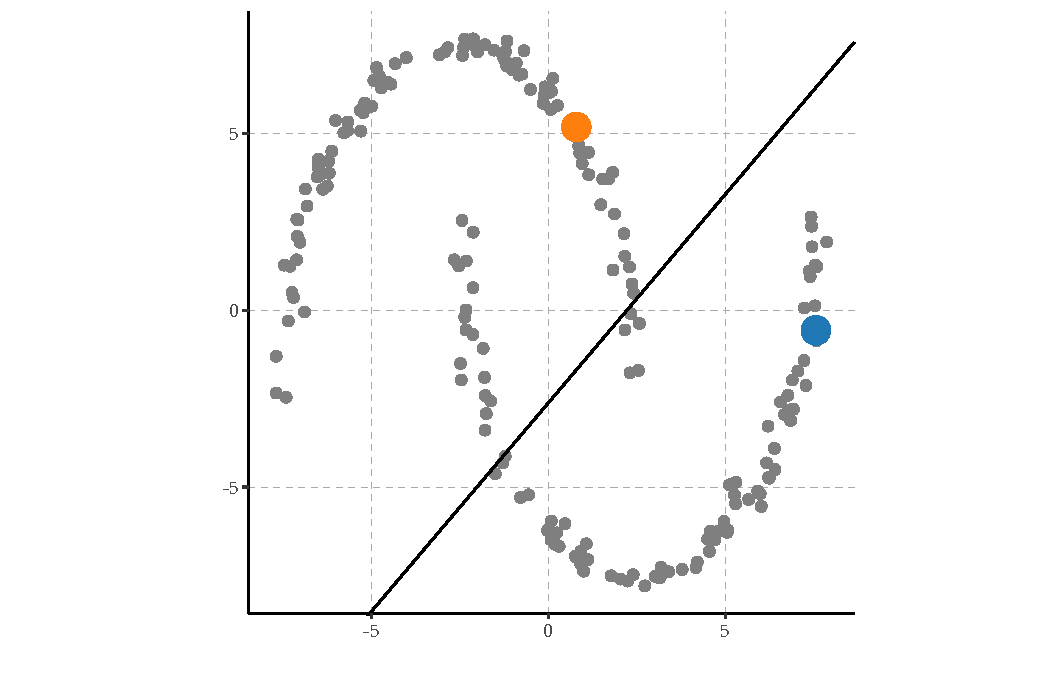
\includegraphics[width=\maxwidth]{figure/stylizedexample1-1} \caption[Classification example with one training object for each class and a larger number of unlabeled objects]{Classification example with one training object for each class and a larger number of unlabeled objects. The solid line corresponds to a supervised logistic regression classifier. The configuration of the unlabeled data could suggest the decision boundary should be updated.}\label{fig:stylizedexample1}
\end{figure}


\end{knitrout}

The example in \Cref{fig:stylizedexample2} is similar but deals with a regression problem: the output is a continuous value instead a discrete class. Again, the structure of the unlabeled data may suggest (to some) that the prediction function should be updated to take into account that the predictions change smoothly over the area where many unlabeled objects reside, but changes more rapidly where few unlabeled objects have been observed. In this case, it could mean we want to update the predictions in the `tails' to values more closely aligned with the labeled example that is closest when measured when only considering paths through high density areas.

Note that in both cases the labeled data do not tell us whether these assumptions that lead to changes to the decision boundary are true. We intuit them on top of the labeled information that is already there.

\begin{knitrout}
\definecolor{shadecolor}{rgb}{1, 1, 1}\color{fgcolor}\begin{figure}
\subfloat[Observed data\label{fig:stylizedexample21}]{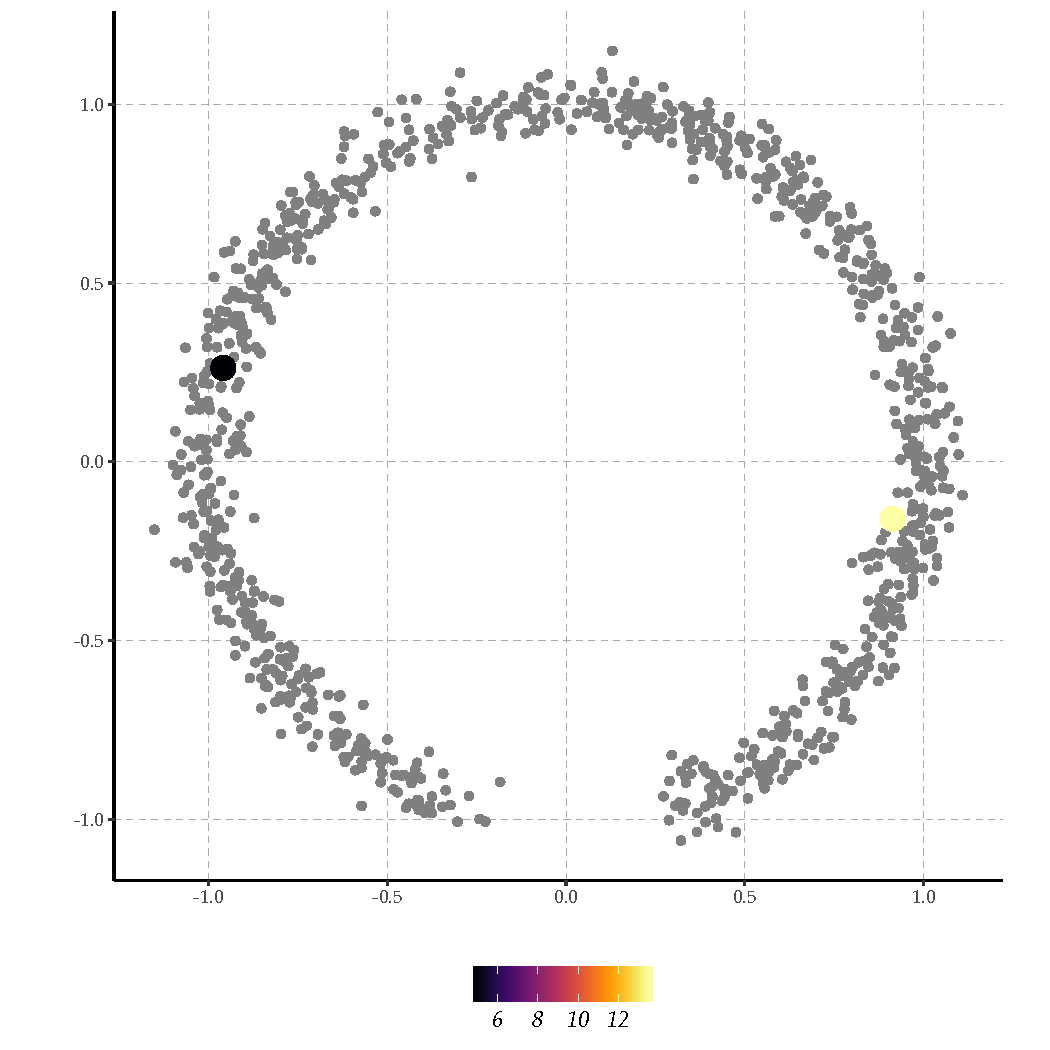
\includegraphics[width=0.49\linewidth]{figure/stylizedexample2-1} }
\subfloat[Predictions\label{fig:stylizedexample22}]{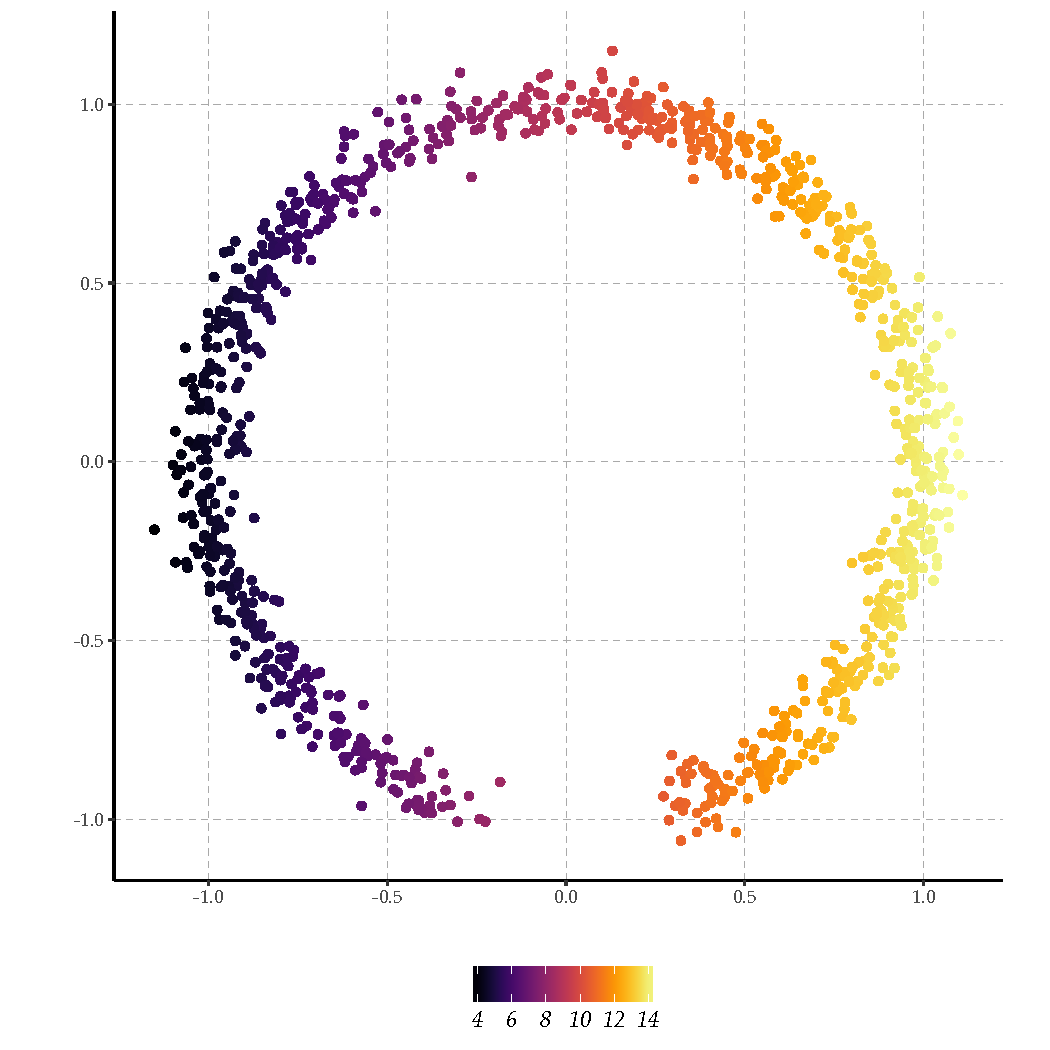
\includegraphics[width=0.49\linewidth]{figure/stylizedexample2-2} }\caption[Regression example where the unlabeled data could convince one to update the estimated function by assuming the two ends of arcs are more likely to have a value similar to objects that are close in the intrinsic geometry indicated by the unlabeled data]{Regression example where the unlabeled data could convince one to update the estimated function by assuming the two ends of arcs are more likely to have a value similar to objects that are close in the intrinsic geometry indicated by the unlabeled data.}\label{fig:stylizedexample2}
\end{figure}


\end{knitrout}

A second argument for the merit of unlabeled data is that humans also do not seem to learn in a strictly supervised way. Both children and adults do not require constant feedback when learning to recognize objects or improve their judgement. \citet[Ch.7]{Zhu2009} offer an overview and discussion of some of the research in cognitive science that studies the question whether humans actually use unlabeled data to adapt their judgement. Results are mixed, but suggest that in simple experimental settings humans use semi-supervised learning to solve tasks. 

However, even if semi-supervised learning is used by humans as a heuristic in many of the practical problems nature throws at us, this does not necessarily mean that it is possible in general, nor does it clearly demarcate when semi-supervised learning has merit.

Lastly, a very practical argument for the use of unlabeled data is that in some applications, semi-supervised methods have shown to be able to improve over supervised solutions. A well-known example is \cite{Nigam2000} who showed this early on in a text classification example. It has also led to improved performance of estimators in bioinformatics \citep{Weston2005,Kall2007,Kasabov2003,Patel2015a}, nuclear power plant monitoring \citep{Ma2015,Moshkbar-bakhshayesh2016}, food quality \citep{Dean2006} and remote sensing \citep{Gomez-Chova2008}, among other applications. For instance, promising results in computer vision are shifting interest to leveraging abundant unlabeled data \cite{Rasmus2015}. 

\section{The Need for Safe Semi-supervised Learning}
Unfortunately, using unlabeled data is not necessarily harmless. Consider \Cref{fig:plotfail}. It shows learning curves for two datasets, one for which adding unlabeled data to the training process improves classification performance for a specific classifier, yet, on the other dataset, performance only gets worse as we add more unlabeled data.

\begin{knitrout}
\definecolor{shadecolor}{rgb}{1, 1, 1}\color{fgcolor}\begin{figure}
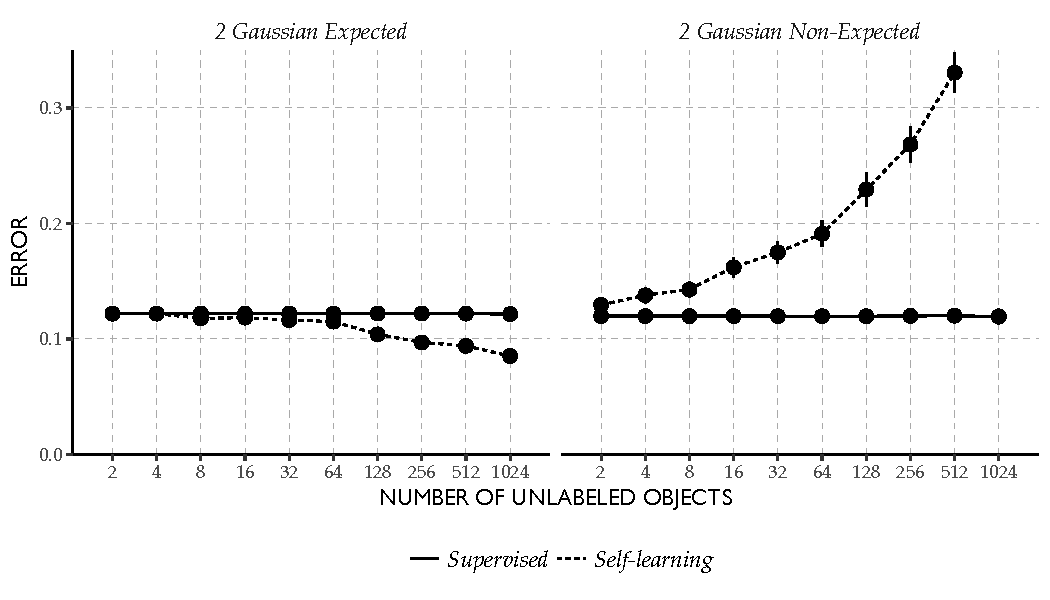
\includegraphics[width=\maxwidth]{figure/plotfail-1} \caption[Example where semi-supervised learning improves performance (left) and reduces performance (right) as compared to the supervised alternative]{Example where semi-supervised learning improves performance (left) and reduces performance (right) as compared to the supervised alternative.}\label{fig:plotfail}
\end{figure}


\end{knitrout}

This behaviour has been observed empirically on numerous occasions, see, for instance, \citep{Elworthy1994} or the references in \citep{Cozman2002}. One could wonder whether these degradations in performance are caused by numerical problems in computing the semi-supervised classifiers or whether this is a more fundamental aspect of semi-supervised learning. \citet{Cozman2003} study this by constructing problems for which generative models, when misspecified, increase the classification error as unlabeled data are added to the training sample, regardless of numerical issues. Note that this is unlike the behaviour we observe in supervised classifiers, where we generally find that adding labeled data increases classification performance, regardless of misspecification. For some exceptions to this general behaviour, see, for instance \cite{Loog2012}.

\section{Arguments for the Limitations of SSL}
Given these negative results, one could argue that it is a priori unlikely that examples of the input alone will tell us anything at all about the outcome given the input. How, for instance, does knowing a certain percentage of web pages have the word `model' in it tell us anything about the probability that a page is about `fashion' or `statistics' given that it contains the word `model'?

\citet{Seeger2001} argues that for discriminative models where we directly model $p_{Y|X}$ (which he calls the diagnostic paradigm), semi-supervised learning is impossible unless one can make useful assumptions about the relationship between the parameters governing the distribution that generates the input vales $X$ and the distribution that generates the labels $Y$ given some $X=\mathbf{x}$. His argument can be illustrated by the graphical model in \Cref{fig:graphicalmodel}(a). The parameters $\theta_X$, corresponding to the data generating distribution of $X$, and $\theta_{Y|X}$, corresponding to the data generating distribution of $Y$ given $X$, are a priori independent. Because of the way the likelihood factorizes, unlabeled data play no role in updating beliefs about $\theta_{Y|X}$ and additionally, learning something about $\theta_X$ should not influence our estimate of $\theta_{Y|X}$. Compare this to the generative model in \Cref{fig:graphicalmodel}(b), where $\theta_X$ and $\theta_{Y|X}$ are dependent if we observe $X$.

\citet{Hansen2009} makes a related argument by constructing the optimal Bayesian predictor for the squared loss, given that we know the prior that nature uses over parameters to generate datasets. He finds that in general this optimal predictor is given by the following solution:
\begin{equation}
\int \int y p(y|x,\theta) d y \frac{p(x,D_l,D_u|\theta) p(\theta)}{\int p(x,D_l,D_u|\theta') p(\theta') d\theta'} d \theta \,, \nonumber
\end{equation}
where $D_l$ is the labeled data set and $D_u$ is the unlabeled dataset and $p(\theta)$ is the true prior on the parameters that is used by nature to generate datasets. Now suppose we split the parameter vector $\theta$ into three sets, one belonging to the conditional distribution $p_{Y|X}$, one belonging to $p_{X}$ and one that is shared between these two. When this shared set is empty, the optimal solution becomes:
\begin{equation}
\int \int y p(y|x,\theta) d y \frac{p(D_l|\theta) p(\theta)}{\int p(D_l|\theta') p(\theta') d\theta'} d \theta \,. \nonumber
\end{equation}
In this case, the solution is the regular Bayesian solution based on the labeled data and the unlabeled data play no role. Only if the two distributions essentially share parameters will unlabeled data play a role in the solution.

If these models correspond exactly to the data generating process, then these arguments hold. Yet these arguments do not tell us anything about the model itself: what are the possibilities of these models if, for instance, the dependence relationships between the variables are different from what the model assumes? \citet{Scholkopf2012} consider this situation more explicitly, by also assuming causal semantics for the models using structural causal models to describe them. They show that indeed, in the model described in \Cref{fig:graphicalmodel}(a), semi-supervised learning can not outperform supervised learning. The main concept in their analysis is that of the causal direction of prediction. If $X$ is the input, $Y$ the output we are interested in predicting and \Cref{fig:graphicalmodel}(a) is a representation of the causal structure of the problem, then we are predicting in the causal direction and semi-supervised learning is impossible, due to so-called \emph{independence of mechanism}. This is assuming there are no other confounding variables. On the other hand, if the true causal model is represented by \Cref{fig:graphicalmodel}(b), we are in the anti-causal prediction scenario and information about $p_X$ is informative about the $p_{Y|X}$.

Summarizing, these arguments depend on the assumption that the models correspond to the true data generating process but tell us little about the possibilities of unlabeled data for a method for which this correspondence is not correct. In practice, however, we often deal with, non-Bayesian, potentially misspecified models and finite amounts of data. Even if unlabeled data are not informative for the true model, this does not guarantee it might not be useful to improve estimates for models used or for finite amounts of data: they may, for instance, suggest what part of the feature space is best served by more accurate predictions from a model with limited complexity.

For example, \citet{Sokolovska2008} show that for logistic regression with discrete input features, if the model is misspecified, information about $p_X$ is informative and leads to an estimator with lower asymptotic variance than the supervised estimator. All in all, model misspecification and finite sample sizes seem to play an under appreciated role in these graphical model analyses of the semi-supervised problem.

\begin{figure}
\centering
\subbottom[Diagnostic Model]{
\begin{tikzpicture}[scale=0.5]
\tikzstyle{main}=[circle, minimum size = 16mm, thick, draw =black!80, node distance = 16mm]
\tikzstyle{connect}=[-latex, thick]
\tikzstyle{box}=[rectangle, draw=black!100]
  \node[main, fill = white!100] (xnode)  {$X$};
  \node[main] (ynode) [right=of xnode] {$Y$};
  \node[main] (thetax) [above=of xnode] {$\theta_X$};
  \node[main] (thetayx) [above=of ynode] {$\theta_{Y|X}$};
  \path (xnode) edge [connect] (ynode)
        (thetax) edge [connect] (xnode)
        (thetayx) edge [connect] (ynode);
\end{tikzpicture}
}%
\quad\quad\quad
\subbottom[Generative Model]{
\begin{tikzpicture}[scale=0.8]
\tikzstyle{main}=[circle, minimum size = 16mm, thick, draw =black!80, node distance = 16mm]
\tikzstyle{connect}=[-latex, thick]
\tikzstyle{box}=[rectangle, draw=black!100]
  \node[main, fill = white!100] (xnode)  {$X$};
  \node[main] (ynode) [right=of xnode] {$Y$};
  \node[main] (thetax) [above=of xnode] {$\theta_{X|Y}$};
  \node[main] (thetayx) [above=of ynode] {$\theta_{Y}$};
  \path (ynode) edge [connect] (xnode)
        (thetax) edge [connect] (xnode)
        (thetayx) edge [connect] (ynode);
\end{tikzpicture}
}
\caption{Graphical model representations of two modelling paradigms. When assuming causal semantics and Y as being the outcome of interest,  (a) is an example of prediction in the causal direction, while (b) is prediction in the anti-causal direction.}
\label{fig:graphicalmodel}
\end{figure}

\citet{Ben-David2008} take a learning theory approach to identify the usefulness of unlabeled data in the ``no prior knowledge'' setting, meaning the setting where we do not make assumptions about the link between $p_{Y|X}$ and $p_{X}$. They show that for some simple concept classes over the real line, algorithms that use unlabeled data can not give sample size guarantees that are more than a constant factor better than supervised algorithms. Sample size guarantees are guarantees that the algorithm will make an error of at most $\epsilon$ with probability $\delta$ for a given sample size. They conjecture that this finding holds more generally for other semi-supervised scenarios as well, but it remains an open question. They also suggest that the problem with the prior knowledge assumed for many semi-supervised approaches is that it is untestable and give examples when these assumptions can lead to deteriorated performance compared to supervised empirical risk minimization.

The general consensus from these analyses is that unlabeled data will not lead to improved performance unless there is a link between $p_X$ and $p_{Y|X}$. Most of these analyses, however, depend on the assumption that the model is correctly specified or depend on asymptotic arguments. In practice, our model will not perfectly fit the data and we have a limited number of observations. Moreover, even though some results suggest that semi-supervised learning without assumptions is only possible when the model is misspecified, this is exactly the situation where semi-supervised learning might fail. Can we instead consider whether semi-supervised learning is possible based on the properties of the method, rather than the data generating process and can we guarantee that improvement happens in a safe way in a setting where we have limited data?

\section{Assumptions We Might Need}
While the research covered so far does still not fully characterize the possibilities of semi-supervised learning in the general case, many authors suggest that assumptions are needed that link knowledge about $p_X$ to knowledge about $p_{Y|X}$. Let us quickly cover the assumptions that dominate semi-supervised learning research: identifiable mixture distributions, the manifold assumption, the clustering assumption and the low-density assumption and consider what we might learn when we make such assumptions.

A classic analysis by \citet{Castelli1995} shows that if we assume identifiable mixture models where each component of the mixture belongs to one class, and  we have an infinite amount of unlabeled samples, a single labeled sample gives a classification risk of $2R^*(1-R^*)$, with $R^*$ being the minimum attainable classification error. Adding more labeled examples allows convergence to this Bayes error with rate: 
$$
R(N_l,N_u=\infty) - R^* = \exp(-l K + o(l)) \,,
$$
with $K$ being a measure of similarity between the class conditional distributions. The idea behind this analysis is that the unlabeled data will identify the different decision regions, while the labeled data only have to be used to identity which decision region belongs to which class.

This may suggest labeled data are exponentially more valuable than unlabeled data, but note the exponential value comes after we used the infinite amount of unlabeled data. \citet{Castelli1996} extend this analysis to the finite sample case, for a simpler situation where we either know the class conditional distribution for each class and only need to estimate the class prior or we know the class conditionals but not the assignment of class conditionals to classes. In the former case, the value of examples in reducing the risk is proportional to the Fisher information of the labeled and unlabeled data, where the value of the labeled data are strictly larger than the unlabeled data. In the second scenario, a difference in the value of both types of information can also be shown to hold, although in this case, no learning is possible without labeled examples.

An important aspect highlighted in these analyses is that the role the unlabeled data play is in reducing the number of possible decision functions, between which we can then efficiently find the correct one with limited labeled data. This idea is used in many of the following analyses as well.

\citet{Lafferty2007} consider the utility of the assumption of smoothness, where one assumes a regression function is smooth in regions where $p_X(\mathbf{x})$ is high. They find that the manifold assumption (see below) alone is sufficient, but that a class of algorithms that attempts to use the manifold and smoothness assumptions together do not offer better convergence rates in terms of the squared error than supervised procedures. They do construct, however, new approaches that use either of these assumptions individually that do have improved convergence rates by using the unlabeled data.

\citet{Niyogi2013} consider the assumptions that the labeling function varies smoothly over the intrinsic manifold of the data. He shows that for a particular class of problems, exemplified by different embeddings of circles in Euclidean space, knowledge of the manifold allows one to learn the correct function efficiently, meaning the approximation error converges to zero at a fast rate. At the same time, for this class of problems, there is no supervised algorithm for which convergence can be guaranteed for all distributions in the class. The intuition behind why knowledge of the manifold will help identify the correct conditional distribution is that it reduces the space of potential solutions, after which regular convergence results guarantee fast convergence.

Similarly, \citet{Singh2008} apply minimax lower bounding techniques to a version of the cluster assumption, where outcomes or conditional distributions are assumed to be smooth within a cluster, or decision set. They show that if these decision sets can be found using the unlabeled data and if a supervised learner with knowledge of these sets outperforms one without this knowledge, gathering unlabeled samples at a fast enough rate guarantees improved performance. Using a specific regression scenario, they show how the merit of unlabeled examples depends strongly on the margin between the decision sets and the amount of unlabeled data.

Based on the potential of semi-supervised methods to decrease performance compared to supervised procedures, \citet{Li2015} construct a safe version of the semi-supervised support vector machine by employing a low-density separation assumption. The assumption is that the true decision boundary is situated in regions of low-density in the feature space. The idea behind this approach is to generate a set of low-density separators and pick one conservatively. If indeed this set contains the true solution, they are able to show procedure will improve in terms of performance compared to the supervised procedure.

In summary, given that we can make assumptions that link $p_X$ and $p_{Y|X}$, it is possible to prove unlabeled data have some value. But as \citet{Ben-David2008} and others have pointed out, checking these assumptions is often difficult or impossible. If we can not be sure these assumptions are true and the unlabeled data may lead to a procedure with reduced performance, perhaps we should avoid them completely. The view taken in this thesis is then to forego these assumptions, and find out whether semi-supervised learning is still possible for this case and what performance guarantees this allows us to derive.

In this way, the work presented is inspired by, and builds on, earlier work in \citet{Loog2010,Loog2014b,Loog2014a}, who attempt to work out the intrinsic constraints posed by some supervised models without introducing constraints. These constraints then also have to hold for any semi-supervised solution. While in their work, these constraints need to be explicitly derived, in the framework presented in this thesis constraints are implicitly defined, and the limit of their usefulness investigated.

\section{Research Questions}
Based on these considerations, the main questions that we will address in this thesis are the following:
\begin{itemize}
\item Can we construct a (non-trivial) semi-supervised version of some supervised classifier without making additional assumptions that were not inherent in the supervised method?

\item For these classifiers, in what sense can we guarantee that they (safely) improve over the supervised alternative?

\item Can we prove this notion of safe semi-supervised learning is (im)possible for other classifiers?
\end{itemize}

During these investigations, some additional questions will come up that we try to address. For instance, why do semi-supervised approaches applied to the unregularized least squares classifier fail when the dimensionality of the input sample is larger than the size of the sample? And what is a proper definition for self-learning approaches to the least squares classifier that may not work in all cases, but give decent performance in many cases? 

To answer these and other questions, we will rely on both mathematical analalysis as well as results from computational simulations and experiments. What is the role of reproducibility of these experiments in pattern recognition research and how do we ensure it?

\section{Important Conceptual Constructs}

Before continuing with the outline of the thesis, we will cover some of the most important concepts in the thesis that we will use to address the research question, which may help put things in perspective.

\subsection{Surrogate losses}

The loss $L$ that is optimized in the ERM framework outlined above, does not directly correspond to the goal that many people have in mind when training a classifier. To evaluate a classifier, one often considers the error rate, the area under the ROC curve, F-score or various other measures of performance. Optimizing these losses directly poses numerical difficulties. Therefore so-called surrogate losses are usually employed which upper bound the error rate while being computationally tractable, or easier to analyse mathematically.

\subsection{Margin-based Losses}
One particular class of these losses are so-called margin-based losses. These are losses of the form $\phi(y f(\mathbf{x}))$ where $y \in \{-1,+1\}$ is the encoding of the binary class label. Margin-based losses have been studied extensively in the context of their convergence properties. \citet{Bartlett2006}, for instance, show that for any convex $\phi$ with $\phi$ differentiable at $0$ and $\phi'(0)<0$ then $\phi$ is \emph{classification calibrated}, which implies that if a sequence of measurable functions converges to the optimal risk in terms of this margin-based loss, this sequence also converges to the Bayes risk in terms of classification error \cite[Theorem 1.3c]{Bartlett2006}. Various well-known and often used classification methods can be formulated as the risk minimization of some margin-based loss, such as support vector machines, forms of boosting, logistic regression and the least squares classifier.

\subsection{On Squared Loss}
The least squares classifier can be defined as the decision function that minimizes the squared loss on the training data. For linear classifiers, one could also interpret this as encoding the vector of class labels as a numeric vector and using this as the dependent variable in linear regression.

In this thesis we consider the squared loss extensively. One could argue, however, that this loss is antiquated, unsuitable or somehow non-optimal for classification \cite{Ben-David2012}. Yet the squared loss shares many properties with other commonly used loss functions. For instance, it is a margin-based loss and it is classification calibrated (see above). Moreover, as many have observed, empirically it gives similar performance in terms of the error rate as other losses on many example datasets \cite{Rifkin2003, Poggio2003, Zhang2004, Rasmussen2005}.  \citet{Rifkin2002} even notes that ``the choice between SVM and RLSC [regularized least squares classifier] should be based on computational tractability considerations''. One particular advantage of the squared loss is that it leads to a closed-form solution of the classifier which makes it easier to analyse theoretically, a property we will make use of repeatedly throughout the thesis.

\subsection{Projected Estimators}
The main concept behind the proposed robust semi-supervised learning approaches in this thesis is that of projecting a supervised classifier onto a set of potential solutions defined by the unlabeled data. We will refer to this set as the constraint set since it encodes the constraints that the unlabeled data put on the potential solutions.

Projecting estimators onto sets of constraints has been considered for other problems in statistics. For instance, the case where one knows the true solution adheres to certain linear inequality constraints \citep{Schmidt1995, Schmidt1996} or constraints that form some convex set \citep{Stahlecker1996}. \citet{Schmidt1995} prove, for example, that the projection of any estimator to the set of linear inequality constraints leads to an equal or improved estimator: one that is `closer' to the true solution and dominates the non-projected estimator, given that the true solution is within the set of constraints. 

In the setting considered in our work, however, we do know such constraints, all we have is labeled and unlabeled objects. How, then, can we apply these projections to the semi-supervised setting? More specifically:
\begin{enumerate}
\item What is the estimator that is to be projected?
\item How do we form the constraint set?
\item How do we measure what it means for solutions to be `close'?
\item How do we choose a solution from the constraint set?
\end{enumerate}
As we will elaborate in the rest of this thesis, in our semi-supervised solutions, we propose the following answers to these questions: (1) The solution to be projected is the supervised solution. (2) The constraint set is formed implicitly by all possible supervised classifiers we could get by assigning a potential labeling to the unlabeled objects. (3) The measure depends on the loss we are interested in minimizing and (4) we find the semi-supervised solution either through minimizing the supervised loss within the constraint set (\Cref{chapter:icls,chapter:iclda}) or minimizing a particular distance measure that ensures we always get a better estimator (\Cref{chapter:projection}).

\begin{knitrout}
\definecolor{shadecolor}{rgb}{1, 1, 1}\color{fgcolor}\begin{figure}
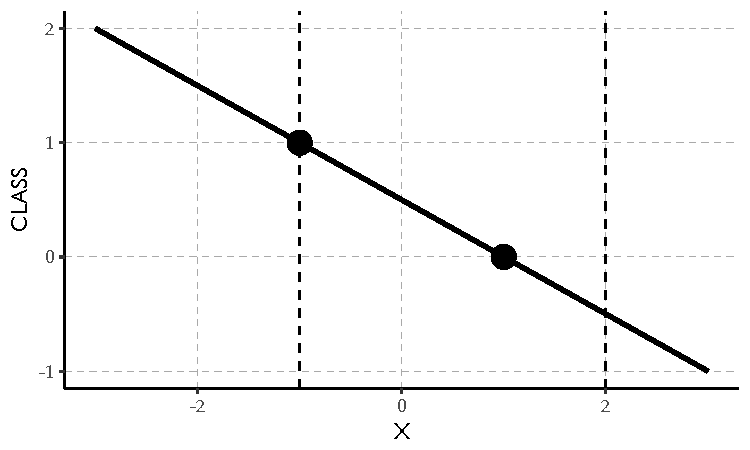
\includegraphics[width=\maxwidth]{figure/coverexample-1} \caption[Dataset used to illustrate the projection example that corresponds to the projection illustrated on the cover of the thesis]{Dataset used to illustrate the projection example that corresponds to the projection illustrated on the cover of the thesis. The circles indicate the locations and labels of the two labeled objects. The solid line indicates the supervised decision function, while the dashed lines correspond to the locations of the two unlabeled objects}\label{fig:coverexample}
\end{figure}


\end{knitrout}
To give a preview of what such a procedure looks like geometrically and to explain the illustration on the cover of this thesis, consider \Cref{fig:coverexample}. In this one dimensional classification problem, we show  the labels for two objects, the locations of the two unlabeled objects and the supervised linear decision function. We can represent this supervised solution by two numbers: its intercept and its slope. This is represented by the white dot on the cover. Additionally, we can try every possible labeling of the unlabeled objects (including all partial assignments to the two classes), calculate the intercept and slope of the resulting classifier and plot this set of solutions. This constraint set of all classifiers possible by some labeling of the unlabeled data is depicted by the white area on the cover. The ellipses show the iso-distance lines for the distance measure used to carry out the projection, while the light-blue dot is the projected solution, corresponding to our semi-supervised solution. As you can see by the iso-distance lines from the true solution (the dark-blue dot), this solution is closer in terms of this distance measure, than the supervised solution was. If this distance measure is appropriately chosen, this distance will correspond to the loss we are interested in minimizing.
This last statement shows the power of this projection approach as it leads to a simple proof that guarantees the semi-supervised solution is always better than the supervised solution, as we will show in \Cref{chapter:projection}.

\section{A Map but not the Territory}
Before we dive into the specifics, we will look at the outline of the chapters and indicate how they are related. In part one of the thesis, we introduce the use of constraints and projections in semi-supervised learning. In \Cref{chapter:icls}, we construct a semi-supervised classifier based on the idea of implicit constraints. Despite the fact that this approach does not require additional assumptions about the unlabeled data that were not already present in the supervised classifier, we show it is able to improve the supervised classifier using the unlabeled data in experiments on benchmark datasets and, particularly, performs robustly, meaning it almost never degrades in performance compared to the supervised alternative. Additionally, we prove, for 1D problems without intercept and infinite unlabeled data, that this semi-supervised approach will always outperform the supervised counterpart. In \Cref{chapter:iclda}, we apply this same methodology of implicit constraints to a different classifier, linear discriminant analysis, to show how the approach extends to other classifiers. 

While the approach in \Cref{chapter:icls} is guaranteed to improve over the supervised learner in a very restricted setting, in \Cref{chapter:projection} we extend these results to the more general multivariate setting for a different, but related, procedure. We interpret this procedure as a projection of the supervised solution onto the implicit constraints set. For a particular distance measure we can then prove this procedure is always better than the supervised solution when evaluated in terms of the surrogate loss on the labeled and unlabeled data. 

Since these performance guarantees are in terms of the surrogate loss, instead of the classification error or some other common performance measure, in part two of the thesis, we consider the importance of these surrogate losses. In \Cref{chapter:quantifying}, we discuss situations in which it is insightful to consider the surrogate loss to study the behaviour of classifiers.
In \Cref{chapter:marginbased}, we consider these surrogate losses to prove for a particular class of classifiers based on margin-based losses that under certain conditions, safe semi-supervised learning is impossible. We also show for which cases improvement guarantees are possible, covering, among other cases, the results we obtained in \Cref{chapter:projection}.

In \Cref{chapter:optimistic}, we turn away from the pessimism considered in \Cref{chapter:projection} to consider how to properly define an optimistic version of the least squares classifier. We show how to define a soft-label self-learning variant of the least squares classifier and study its properties.

In \Cref{chapter:peaking}, then, we cover the peaking phenomenon in semi-supervised learning, that we ran into during some of the experiments in this thesis and which was briefly covered in \Cref{chapter:icls}. We show, for a simple semi-supervised least squares approach, where this behaviour originates and why it is more extreme than in the supervised setting.

The final part of this thesis, part three, is devoted to questions concerning the reproducibility of the results of the rest of the thesis. \Cref{chapter:reproducing} discusses the concepts of reproducibility and replicability in the pattern recognition context and offers a case study of reproducing \Cref{chapter:optimistic}, as well as additional results. \Cref{chapter:rssl} describes the toolbox we implemented to produce all the results in this thesis, that can be used to reproduce these and other results in semi-supervised learning research.

We end with a discussion of the findings of this thesis.
\afterpage{\newpagecolor{ThesisLight}}
\mainmatter*
\nopagebreak
% standard part pages should be suppressed, custom part page used instead
\renewcommand{\printpartname}{}
\renewcommand{\printpartnum}{}
\renewcommand{\printparttitle}{\phantom}

% Custom part page for Part I
% \cleartoverso
% \null
% \thispagestyle{empty}
\afterpage{\restorepagecolor}
% \newpage
\renewcommand{\mypartpic}{cover/part1.pdf}
\AddToShipoutPicture{\PartPic}
\part{CONSTRAINTS \& PROJECTIONS}
\afterpage{\restorepagecolor}
\ClearShipoutPicture


\chapter[Implicitly Constrained Semi-supervised Least Squares Classification]{Implicitly Constrained Semi-supervised\\Least Squares Classification}
\chaptermark{Implicitly Constrained Least Squares}
\label{chapter:icls}
\blfootnote{This chapter appeared as: Krijthe, J.H. \& Loog, M., 2017. Robust Semi-supervised Least Squares Classification by Implicit Constraints. Pattern Recognition, 63, pp.115–126. An earlier, shorter, version of this work appeared as: Krijthe, J. H., \& Loog, M. (2015). Implicitly Constrained Semi-Supervised Least Squares Classification. In E. Fromont, T. De Bie, \& M. van Leeuwen (Eds.), Advances in Intelligent Data Analysis XIV. Lecture Notes in Computer Science, vol 9385. (pp. 158–169).}

\begin{abstract}
We introduce the implicitly constrained least squares (ICLS) classifier, a novel semi-supervised version of the least squares classifier. This classifier minimizes the squared loss on the labeled data among the set of parameters implied by all possible labelings of the unlabeled data.
Unlike other discriminative semi-supervised methods, this approach does not introduce explicit additional assumptions into the objective function, but leverages implicit assumptions already present in the choice of the supervised least squares classifier.
This method can be formulated as a quadratic programming problem and its solution can be found using a simple gradient descent procedure. 
We prove that, in a limited one dimensional setting, this approach never leads to performance worse than the supervised classifier.
Experimental results show that also in the general multidimensional case performance improvements can be expected, both in terms of the squared loss that is intrinsic to the classifier, as well as in terms of the expected classification error.
\end{abstract}

\section{Introduction}
We consider the problem of semi-supervised learning of binary classification functions. As in the supervised paradigm, the goal in semi-supervised learning is to construct a classification rule that maps objects in some input space to a target outcome, such that future objects map to correct target outcomes as well as possible. In the supervised paradigm this mapping is learned using a set of $\Nlab$ training objects and their corresponding outputs. In the semi-supervised scenario we are given an additional and often large set of $\Nunl$ unlabeled objects. The challenge of semi-supervised learning is to incorporate this additional information to improve the classification rule.

The goal of this work is to build a semi-supervised version of the least squares classifier that is robust against deterioration in performance meaning that, at least in expectation, its performance is not worse than supervised least squares classification.
While it may seem like an obvious requirement for any semi-supervised method, current approaches to semi-supervised learning do not have this property. 
In fact, performance can significantly degrade as more unlabeled data is added, as has been shown in \citep{Cozman2006,Cozman2003}, among others.
This makes it difficult to apply these methods in practice, especially when there is a small amount of labeled data to identify possible reduction in performance.
A useful property of any semi-supervised learning procedure would therefore be that its performance does not degrade as we add more unlabeled data.
Additionally, many semi-supervised learning procedures are formulated as hard-to-optimize, non-convex objective functions. 
A more satisfactory state of affairs for semi-supervised classification would therefore be methods that are easier to train and that, on average, do not lead to worse classification performance than their supervised alternatives.

We present a novel approach to semi-supervised learning for the least squares classifier that we will refer to as implicitly constrained least squares classification (ICLS). ICLS leverages implicit assumptions present in the supervised least squares classifier to construct a semi-supervised version. This is done by minimizing the supervised loss function subject to the constraint that the solution has to correspond to the solution of the least squares classifier for some labeling of the unlabeled objects.

As this work is specifically concerned with least squares classification, we note several reasons why this is a particularly interesting classifier to study: 
First of all, the least squares classifier is a discriminative classifier. 
Some have claimed semi-supervised learning without additional assumptions is impossible for discriminative classifiers \citep{Seeger2001,Singh2008}. Our results show this does not strictly hold. 

Secondly, the closed-form solution for the supervised least squares classifier allows us to study its theoretical properties. In particular, in the univariate setting without intercept and assuming perfect knowledge of $P_X$, the distribution of the feature, we show this procedure \emph{never} gives worse performance in terms of the squared loss criterion compared to the supervised least squares classifier. Moreover, using the closed-form solution we can rewrite our semi-supervised approach as a quadratic programming problem, which can be solved through a simple gradient descent with boundary constraints.

Lastly, least squares classification is a useful and adaptable classification technique  allowing for straightforward use of, for instance, regularization, sparsity penalties or kernelization \citep{Hastie2009,Poggio2003,Rifkin2003,Suykens1999,Tibshirani1996}. 
Using these formulations, it has been shown to be competitive with state-of-the-art methods based on loss functions other than the squared loss \citep{Rifkin2003} as well as computationally efficient on large datasets \citep{Bottou2010}.

This work builds on \citep{Krijthe2015} and offers a more complete exposition: we show ICLS can be formulated  as a quadratic programming problem, we extend the experimental results section by including an alternative semi-supervised procedure, adding additional datasets and discussing the ‘peaking’ phenomenon. Moreover, we extend the theoretical result with conditions when one is likely to see improvement of the proposed approach over the supervised classifier.

The main contributions of this paper are
\begin{itemize}
  \item A novel convex formulation for robust semi-supervised learning using squared loss (Equation \ref{icls})
  \item A proof that this procedure never reduces performance in terms of the squared loss for the 1-dimensional case without intercept (Theorem \ref{theorem:1d})
  \item An empirical evaluation of the properties of this classifier (Section \ref{section:empiricalresults})
\end{itemize}

The rest of this paper is organized as follows. 
Section \ref{section:relatedwork} gives an overview of related work on semi-supervised learning. 
Section \ref{section:overview} gives a high level overview of the method while Section \ref{section:method} introduces our semi-supervised version of the least squares classifier in more detail. 
We then derive a quadratic programming formulation and present a simple way to solve this problem through bounded gradient descent. 
Section \ref{section:theoreticalresults} contains a proof of the improvement of the ICLS classifier over the supervised alternative. This proof is specific to classification with a single feature, without including an intercept in the model. For the multivariate case, we present an empirical evaluation of the proposed approach on benchmark datasets in Section \ref{section:empiricalresults} to study its properties. The final sections discuss the results and conclude.

\section{Related Work} 
\label{section:relatedwork}
Many diverse approaches to semi-supervised learning have been proposed   \citep{Chapelle2006,Zhu2009}. While semi-supervised techniques have shown promise in some applications, such as document classification \citep{Nigam2000}, peptide identification \citep{Kall2007} and cancer recurrence prediction \citep{Shi2011}, it has also been observed that these techniques may give performance worse than their supervised counterparts. See for instance \citep{Cozman2006,Cozman2003}, for an analysis of this problem, and \citep{Elworthy1994} for a practical example in part-of-speech tagging.
In these cases, disregarding the unlabeled data would lead to better performance. 

Some \citep{Goldberg2009,Wang2007a} have argued that \emph{agnostic} semi-supervised learning, which \citet{Goldberg2009} defines as semi-supervised learning that is at least no worse than supervised learning, can be achieved by cross-validation on the limited labeled data. 
Agnostic semi-supervised learning follows if we only use semi-supervised methods when their estimated cross-validation error is significantly lower than those of the supervised alternatives.
As the results of \citet{Goldberg2009} indicate, this criterion may be too conservative: given the small amount of labeled data, a semi-supervised method will only be preferred if the difference in performance is very large. 
If the difference is less distinct, the supervised learner will always be preferred and we potentially ignore useful information from the unlabeled objects. 
Moreover, this cross-validation approach can be computationally demanding. 

\subsection*{Self-Learning}
A simple approach to semi-supervised learning is offered by the self-learning procedure \citep{McLachlan1975} also known as Yarowsky's algorithm (see \citep{Abney2004} and \citep{Yarowsky1995}) or retagging \citep{Elworthy1994}.
Taking any classifier, we first estimate its parameters on only  the labeled data. 
Using this trained classifier we label the unlabeled objects and add them, or potentially only those we are most confident about, with their predicted labels to the labeled training set. 
The classifier parameters are re-estimated using these labeled objects to get a new classifier. 
One iteratively applies this procedure until the predicted labels of the unlabeled data no longer change.

One of the advantages of this procedure is that it can be applied to any supervised classifier.
It has also shown practical success in some application domains, particularly document classification \citep{Nigam2000,Yarowsky1995}.
Unfortunately, the process of self-training can also lead to severely decreased performance, compared to the supervised solution \citep{Cozman2006,Cozman2003}. 
One can imagine that once an object is incorrectly labeled and added to the training set, its incorrect label may be reinforced, leading the solution away from the optimum. 
Self-learning is closely related to expectation maximization (EM) based approaches \citep{Abney2004}. Indeed, expectation maximization suffers from the same issues as self-learning \citep{Zhu2009}.
In Section~\ref{section:empiricalresults} we compare the proposed approach to self-learning for the least squares classifier.

\subsection*{Additional Assumptions}
Some semi-supervised methods leverage the unlabeled data by introducing assumptions that link properties of the features alone to properties of the label of an object given its features. Commonly used assumptions are the smoothness assumption: objects that are close in the feature space likely share the same label; the cluster assumption: objects in the same cluster share a label; and the low density assumption enforcing that the decision boundary should be in a region of low data density. 

The low-density assumption is used in entropy regularization \citep{Grandvalet2005} as well as for support vector classification in the transductive support vector machine (TSVM)  \citep{Joachims1999} and closely related semi-supervised SVM (S$^3$VM) \citep{Bennett1998,Sindhwani2006}. 
In these approaches an additional term is added to the objective function to push the decision boundary away from regions of high density. 
Several approaches have been put forth to minimize the resulting non-convex objective function, such as the convex concave procedure \citep{Collobert2006} and difference convex programming \citep{Sindhwani2006,Wang2007}.

In all these approaches to semi-supervised learning, a parameter controls the importance of the unlabeled points. When the parameter is correctly set, it is clear, as \citet{Wang2007a} claims, that TSVM is always no worse than supervised SVM. 
It is, however, non-trivial to choose this parameter, given that semi-supervised learning is most interesting in cases where we have limited labeled objects, making a choice using cross-validation very unstable. 
In practice, therefore, TSVM can also lead to performance worse than the supervised support vector machine, as well will also see in Section~\ref{subsection:crossvalidation}.

\subsection*{Safe Semi-supervised Learning}
\citet{Loog2010,Loog2014b} attempt to guard against the possibility of deterioration in performance by not introducing additional assumptions, but instead leveraging implicit assumptions already present in the choice of the supervised classifier.
These assumptions link parameters estimates that depend on labeled data to parameter estimates that rely on all data. 
By exploiting these links, semi-supervised versions of the nearest mean classifier and the linear discriminant are derived. 
Because these links are unique to each classifier, the approach does not generalize directly to other classifiers. 
The method presented here is similar in spirit, but unlike \citep{Loog2010,Loog2014b}, no explicit equations have to be formulated to link parameter estimates using only labeled data to parameter estimates based on all data. Moreover, our approach allows for theoretical analysis of the non-deterioration of the performance of the procedure.

Aside from the work by \citet{Loog2010,Loog2014b}, another attempt to construct a robust semi-supervised version of a supervised classifier has been made in \citep{Li2011}, which introduces the safe semi-supervised support vector machine (S$^4$VM). 
This method is an extension of S$^3$VM \citep{Bennett1998} which constructs a set of low-density decision boundaries with the help of the additional unlabeled data, and chooses the decision boundary, which, even in the worst-case, gives the highest gain in performance over the supervised solution. 
If the low-density assumption holds, this procedure provably increases classification accuracy over the supervised solution. 
The main difference with the method considered in this paper, however, is that we make no such additional assumptions. We show that even without these assumptions, safe improvements are possible for the least squares classifier.

\subsection*{Semi-supervised Least Squares}
While least squares classification has been widely used and studied \citep{Hastie2009, Poggio2003, Suykens1999}, little work has been done on applying semi-supervised learning to the least squares classifier specifically. For least squares regression, \citet{Little2002} describe an iterative method for handling missing outcomes that was formally proposed by \citet{Healy1956}. In the case of least squares regression, this method has some computational advantages over discarding the unlabeled data but its solution always coincides with the supervised solution. \citet{Shaffer1991} studied the value of knowing $\mathbb{E}[\mathbf{X}^T\mathbf{X}]$, where $\mathbf{X}$ is the $\Nlab \times \featdim$ design matrix containing the feature values for each observation. If we assume the number of unlabeled data points is large, this is similar to the semi-supervised situation. It is shown that if the size of the parameters is small compared to the noise, the variance of a procedure that plugs in $\mathbb{E}[\mathbf{X}^T\mathbf{X}]$ as the estimate of $\mathbf{X}^T\mathbf{X}$ has a lower variance than supervised least squares regression.  As the size of the parameters increases, this effect reverses. In fact, the paper demonstrates that in this semi-supervised setting no best linear unbiased estimator for the regression coefficients exists. In Section \ref{section:empiricalresults}, we compare our approach to using this plug-in estimate by substituting the matrix $\mathbf{X}^T\mathbf{X}$ by a version based on both labeled and unlabeled data. 
A similar plug-in procedure has been used by \citet{Fan2008} for linear discriminant analysis for dimensionality reduction which is closely related to least squares classification. Here the (normalized) total scatter matrix, which plays a similar role to the $\mathbf{X}^T\mathbf{X}$ matrix in least squares regression is exchanged with the more accurate estimate of the total scatter based on both labeled and unlabeled data.

\section{Implicitly Constrained Least Squares Classification}
\label{section:overview}
Given a limited set of $\Nlab$ labeled objects and a potentially large set of $\Nunl$ unlabeled objects, the goal of implicitly constrained least squares classification is to use the latter to improve the solution of the least squares classifier trained on just the labeled data. We start with a sketch of this approach, before discussing the details.

\begin{figure}[ht] 
  \centering
      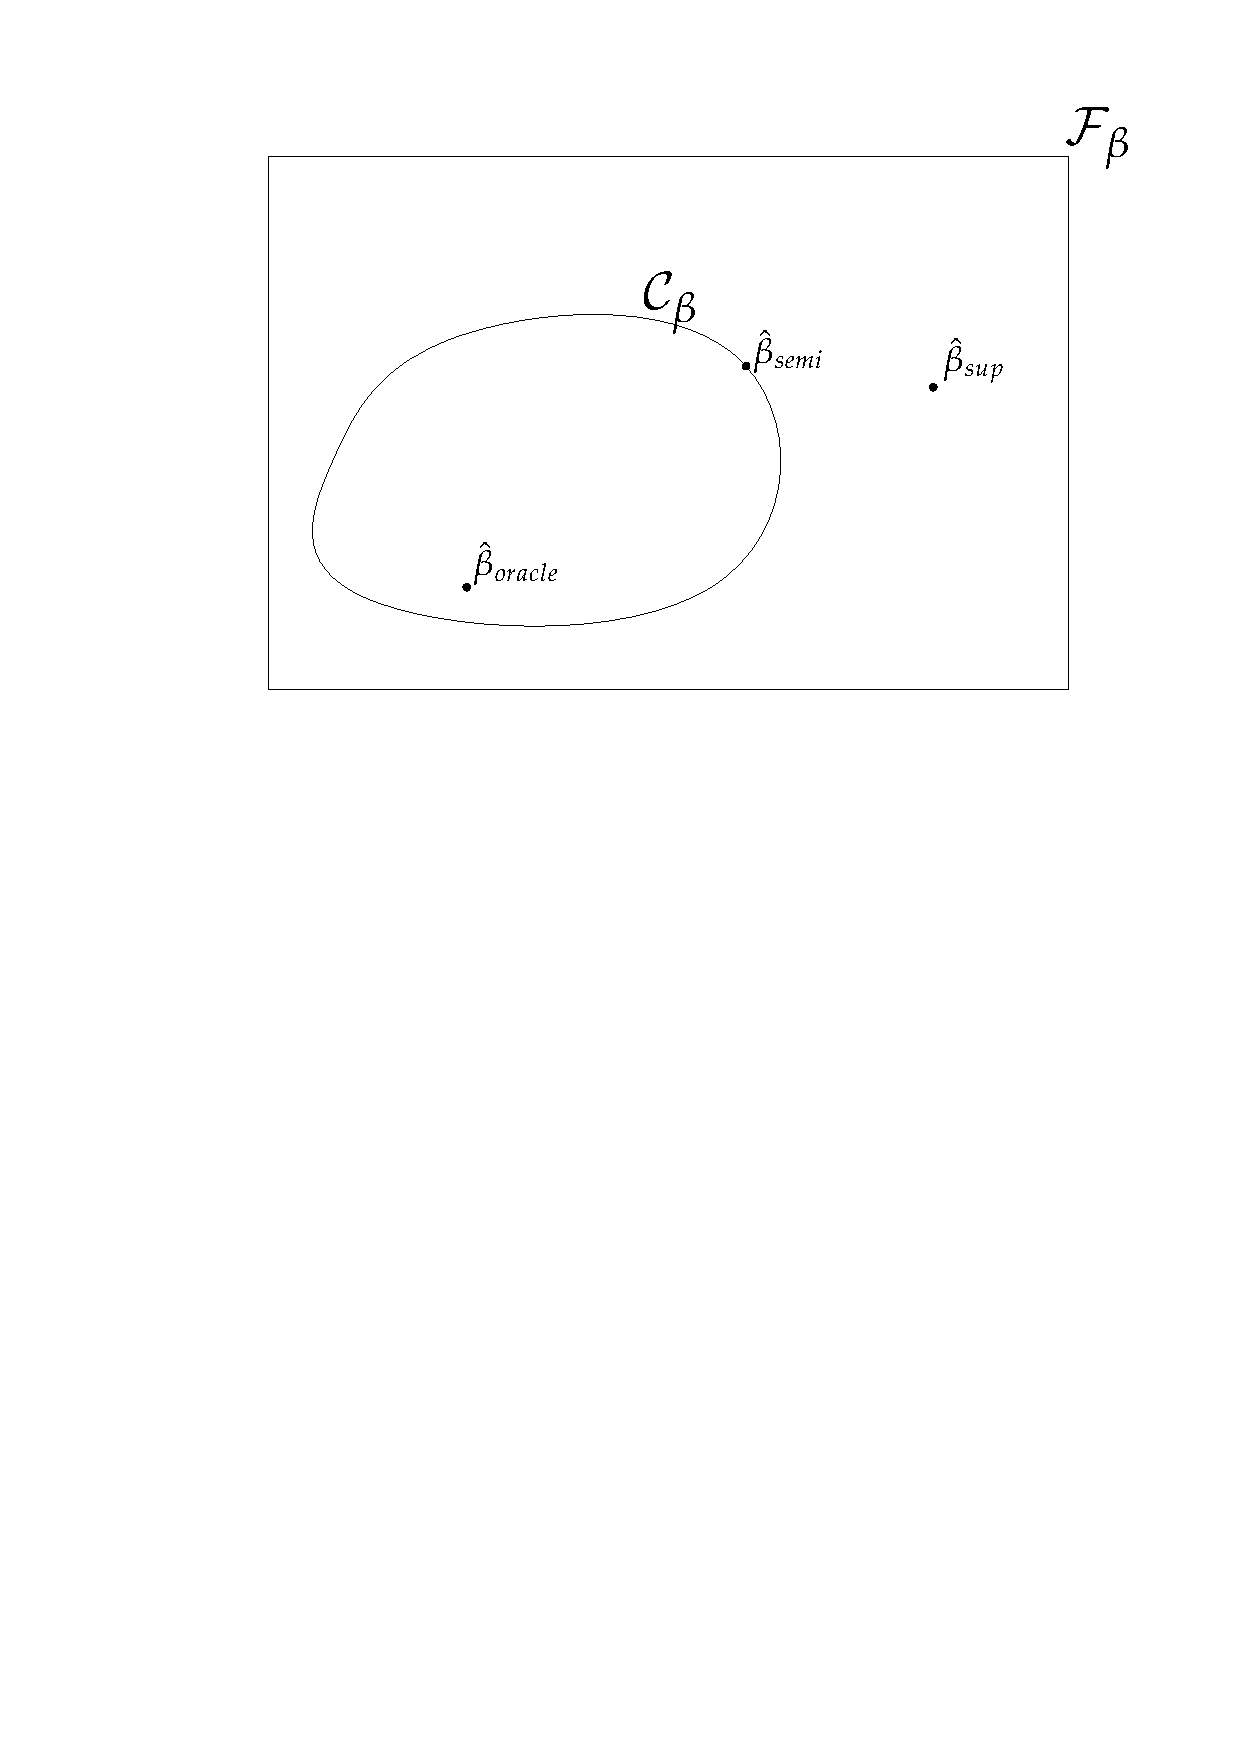
\includegraphics[width=1.0\textwidth]{chapter1/constrainedspace.pdf}
  \caption{A visual representation of implicitly constrained semi-supervised learning. $\mathcal{F}_{\beta}$ is the space of all linear models. $\hat{\beta}_{sup}$ denotes the solution given only a small amount of labeled data. $\Cb$ is the subset of the space which contains all the solutions we get when applying all possible (soft) labelings to the unlabeled data. $\hat{\beta}_{semi}$ is the solution in $\Cb$ that minimizes the loss on the labeled objects. $\hat{\beta}_{oracle}$ is the supervised solution if we would have the labels for all the objects.} \label{fig:constrainedsubset}
\end{figure}

Given the supervised least squares classifier, consider the hypothesis space of all possible parameter vectors, which we will denote as $\mathcal{F}_{\beta}$, see Figure \ref{fig:constrainedsubset}. Given a set of labeled objects, we can determine the supervised parameter vector $\hat{\beta}_{sup}$. Suppose we also have a potentially large number $\Nunl$ of unlabeled objects. Assume that every object has a label, it is merely unknown to us. If these labels were to be revealed, it is clear how the additional objects can improve classification performance: we estimate the least squares classifier using all the data to obtain the parameter vector $\hat{\beta}_{oracle}$. Since this estimate is based on more objects, we expect the parameter estimate to be better. These real labels are unknown, but we can still consider all possible labelings of unlabeled objects, and estimate corresponding parameters based on these imputed labelings. In this way, we get a set of possible parameters for our classifier, which form the set denoted by $\Cb \subset \mathcal{F}_{\beta}$. Clearly one of these labelings corresponds to the real, but unknown, labeling, so one of the parameter estimates in this set corresponds to the solution we would obtain using all the correct labels of both the labeled and unlabeled objects. Because these are the only possible classifiers when the true labels would be revealed, we propose to look within this set $\Cb$ for an improved semi-supervised solution. 

Two issues then remain: how do we choose the best parameters from this set and how do we find these without having to enumerate all possible labelings?

Looking at the first problem, we reiterate that the goal of semi-supervised learning is to find a good classification rule and, therefore, still the obvious way to evaluate this rule is by the loss on the labeled training points. In other words, we choose the classifier from the parameter set that minimizes the squared loss on the labeled points. We will denote this solution by $\hat{\beta}_{semi}$. Note this approach is rather different from other approaches to semi-supervised learning where the loss is adapted by including a term that depends on the unlabeled data points. In our formulation, the loss function is still the regular, supervised loss of our classification procedure.

As for the second issue, after relaxing the constraint that we need hard labels for the data points, we will see that the resulting optimization problem is, in fact, an instantiation of well-studied quadratic programming, which we solve using a simple gradient descent procedure.

\section{Method}
\label{section:method}

\subsection{Supervised Multivariate Least Squares Classification} \label{section:leastsquares}

Least squares classification \citep{Hastie2009,Rifkin2003} is the direct application of well-known ordinary least squares regression to a classification problem. A linear model is assumed and the parameters are minimized under squared loss. Let $\mathbf{X}$ be an $\Nlab \times (\featdim+1)$ design matrix with $\Nlab$ rows containing vectors of length equal to the number of features $\featdim$ plus a constant feature to encode the intercept. Vector $\mathbf{y}$ denotes an $\Nlab \times 1$ vector of  class labels. We encode one class as $0$ and the other as $1$.  The multivariate version of the empirical risk function for least squares estimation is given by

\begin{equation} \label{squaredloss}
\hat{R}(\boldsymbol{\beta}) = \frac{1}{\Nlab} \left\|  \mathbf{X} \boldsymbol{\beta}-\mathbf{y} \right\| _2^2 \, .
\end{equation}
The well-known closed-form solution for this problem is found by setting the derivative with respect to $\boldsymbol{\beta}$ equal to $\mathbf{0}$ and solving for $\boldsymbol{\beta}$, giving
\begin{equation} \label{olssolution}
\boldsymbol{\hat{\beta}}=\left(\mathbf{X}^T \mathbf{X}\right)^{-1} \mathbf{X}^T \mathbf{y} \, .
\end{equation}
In case $\mathbf{X}^T \mathbf{X}$ is not invertible (for instance when $L<(\featdim+1)$), a pseudo-inverse is applied. As we will see, the closed form solution to this problem will enable us to formulate our semi-supervised learning approach in terms of a standard quadratic programming problem, which is easy to optimize.

\subsection{Implicitly Constrained Least Squares Classification} \label{section:icls}

In the semi-supervised setting, apart from a design matrix $\mathbf{X}$ and target vector $\mathbf{y}$, an additional set of measurements $\mathbf{X}_\textrm{u}$ of size $\Nunl \times (\featdim+1)$ \emph{without} a corresponding target vector $\mathbf{y}_\textrm{u}$ is given. In what follows, $\mathbf{X}_\textrm{e}=\begin{bmatrix} \mathbf{X}^T  & \mathbf{X}_\textrm{u}^T \end{bmatrix}^T$ denotes the extended design matrix which is simply the concatenation of the design matrices of the labeled and unlabeled objects.

In the implicitly constrained approach, we incorporate the additional information from the unlabeled objects by searching within the set of classifiers that can be obtained by all possible labelings $\mathbf{y}_\textrm{u}$, for the one classifier that minimizes the \emph{supervised} empirical risk function in Equation~\eqref{squaredloss}. This set, $\Cb$, is formed by the $\boldsymbol{\beta}$s that would follow from training supervised classifiers on all (labeled and unlabeled) objects going through all possible soft labelings for the unlabeled samples, i.e., using all $\mathbf{y}_\textrm{u} \in [0,1]^{\Nunl}$. Since these supervised solutions have a closed form, this can be written as
\begin{equation} \label{constrainedregion}
\Cb := \left\{   \boldsymbol{\beta} = \left( {\XeT} {\Xe} \right)^{-1} {\XeT} \ye: \mathbf{y}_\textrm{u} \in [0,1]^{\Nunl} \right\} \, .
\end{equation}
The soft labeling provides both a relaxation for computational reasons as well as a strategy to deal with label uncertainty. We can interpret these fractions as a type of class posterior for the unlabeled objects. 
This constraint set $\Cb$, combined with the supervised loss that we want to optimize in Equation \eqref{squaredloss}, gives the following definition for implicitly constrained semi-supervised least squares classification:
\begin{equation}
\begin{aligned}
&\operatorname*{argmin}_{\boldsymbol{\beta} \in \Cb} & \hat{R}(\boldsymbol{\beta}) \, .
\end{aligned}
\end{equation}
Since $\boldsymbol{\beta}$ is fixed for a particular choice of $\mathbf{y}_\textrm{u}$ and has a closed form solution, we can rewrite the minimization problem in terms of $\mathbf{y}_\textrm{u}$ instead of $\boldsymbol{\beta}$:
\begin{equation} \label{icls}
\begin{aligned}
& \operatorname*{argmin}_{\mathbf{y}_\textrm{u} \in [0,1]^{\Nunl}} & \frac{1}{\Nlab}  \left\|  \X \left(\XeT \Xe \right)^{-1} \XeT \ye - \mathbf{y} \right\|_2^2 \, . \\ 
\end{aligned}
\end{equation}
The problem defined in Equation \eqref{icls} can be written in a standard quadratic programming  form:
\begin{equation}
\begin{aligned}
& \quad \min_{\mathbf{y}_\textrm{u}} \frac{1}{2} \mathbf{y}_\textrm{u}^T  \mathbf{Q}  \mathbf{y}_\textrm{u} + \mathbf{c}^T \mathbf{y}_\textrm{u}   & \\
& \text{subject to:}  \quad \begin{bmatrix} \mathbf{I}_{\Nunl}  \\ -\mathbf{I}_{\Nunl} \end{bmatrix}  \mathbf{y}_\textrm{u} \leq \begin{bmatrix} \mathbf{1}_{\Nunl}  \\ \mathbf{0}_{\Nunl} \end{bmatrix} & \\
\end{aligned}
\end{equation}
where\footnote{The published version of this paper contains a typo in this equation and the two equations that follow. We corrected this error here.}
\begin{equation}
\begin{aligned}
\mathbf{Q} = & \frac{2}{\Nlab}  \mathbf{X}_\textrm{u} \G \mathbf{X}^T \mathbf{X} \G \mathbf{X}_\textrm{u}^T \,, &\\
\end{aligned} \nonumber
\end{equation}
and
\begin{equation}
\begin{aligned}
\mathbf{c} = & \frac{2}{\Nlab} \mathbf{X}_\textrm{u} \G \mathbf{X}^T \mathbf{X} \G \mathbf{X}^T \mathbf{y} & \\
& - \frac{2}{\Nlab}  \mathbf{X}_\textrm{u} \G \mathbf{X}^T  \mathbf{y} \, . &\\
\end{aligned} \nonumber
\end{equation}
Here, $\mathbf{I}_{\Nunl}$ denotes the $\Nunl \times \Nunl$ identity matrix and $\mathbf{1}_{\Nunl}$ and $\mathbf{0}_{\Nunl}$ denote column vectors of respectively ones and zeros.

Since the matrix $\mathbf{Q}$ is a product of a matrix and its transpose, it is guaranteed to be positive semi-definite. The problem is typically not positive definite because there are different labelings that will lead to one and the same minimum objective. 

The quadratic problem defined above can be solved using, for instance, an interior point method. We have found a gradient descent approach to be easier to apply. Taking the derivative with respect to $\mathbf{y}_\textrm{u}$ and rearranging the terms we find
\begin{align}
\frac { \partial \hat{R} }{ \partial \mathbf{y}_\textrm{u} } = & \ \frac{2}{\Nlab}  \mathbf{X}_\textrm{u} \G \mathbf{X}^T \mathbf{X} \G \mathbf{X}^T \mathbf{y} \nonumber  \\
& +  \frac{2}{\Nlab}  \mathbf{X}_\textrm{u} \G \mathbf{X}^T  \mathbf{X}  \G  \mathbf{X}_\textrm{u}^T \mathbf{y}_\textrm{u}  \nonumber \\
& -  \frac{2}{\Nlab}  \mathbf{X}_\textrm{u} \G \mathbf{X}^T  \mathbf{y} \, . \nonumber
\end{align}

Because of its convexity, this problem can be solved efficiently using a quasi-Newton approach that allows for the  $[0,1]$ box bounds, such as L-BFGS-B \citep{Byrd1995}. Solving for $\mathbf{y}_\textrm{u}$ gives a labeling that we can use to construct the semi-supervised classifier using Equation \eqref{olssolution} by considering the imputed labels as the labels for the unlabeled data.

\section{Theoretical Results}
\label{section:theoreticalresults}
We will examine this procedure by considering it in a limited, yet illustrative setting. In this case we will, in fact, prove that our procedure will \emph{never} give a worse least squares estimate than the supervised solution.
Consider the case where we have just one feature $x$, a limited set of labeled instances and assume we know the probability density function of this feature $f_X$ exactly. 
This last assumption is similar to having unlimited unlabeled data and is also considered, for instance, by \citet{Sokolovska2008}. 
We consider a linear model with no intercept: $y = x \beta$ where $y$, without loss of generality, is set as $0$ for one class and $1$ for the other. 
For new data points, estimates $\hat{y}$ can be used to determine the predicted label of an object by using a threshold set at, for instance, $0.5$.

The expected squared loss, or risk, for this model is given by

\begin{equation} \label{eq:trueloss}
R^*(\beta) = \sum_{y \in \{0,1\}}{ \int_{-\infty}^{\infty}(x \beta - y)^2  f_{X,Y}(x,y)  \mathrm{d}x} \,,
\end{equation}
where $f_{X,Y}=P(y|x) f_X(x)$. We will refer to this as the joint density of $X$ and $Y$. Note, however, that this is not strictly a density, since it deals with the joint distribution over a continuous $X$ and a discrete $Y$. The optimal solution $\beta^\ast$ is given by the $\beta$ that minimizes this risk:

\begin{equation} \label{eq:bayesoptimal}
\beta^* = \operatorname*{argmin}_{\beta \in \mathbb{R}} R^*(\beta) \, .
\end{equation}
We will show the following result:
\begin{theorem}
\label{theorem:1d}
Given a linear model in 1D without intercept, $y = x\beta$, and $f_X$ known, the estimate obtained through implicitly constrained least squares always has an equal or lower risk than the supervised solution: $$R^\ast (\hat{\beta}_{semi}) \le R^\ast (\hat{\beta}_{sup}) \, .$$
In particular, given $1$ labeled sample, if $f_{X,Y}$ is continuous in the feature $X$ with bounded second moment and $f_{X,Y}(0,1) > 0$, then $$\mathbb{E}[R^*(\hat{\beta}_{semi})] < \mathbb{E}[R^*(\hat{\beta}_{sup})] \, .$$
\end{theorem}

\begin{proof}

Setting the derivative of \eqref{eq:trueloss} with respect to $\beta$ to $0$ and rearranging we get

\begin{eqnarray}
&\beta & = \left( \int_{-\infty}^{\infty} { x^2 f_X(x) \mathrm{d}x} \right)^{-1} \sum_{y \in \{0,1\}} \int_{-\infty}^{\infty} { x y f_{X,Y}(x,y) \mathrm{d}x } \\
& & =    \left( \int_{-\infty}^{\infty} { x^2 f_X(x) \mathrm{d}x} \right)^{-1}  \int_{-\infty}^{\infty} { x f_X(x) \sum_{y \in \{0,1\}} y P(y|x) \mathrm{d}x} \\
& & =   \left( \int_{-\infty}^{\infty} { x^2 f_X(x) \mathrm{d}x} \right)^{-1}  \int_{-\infty}^{\infty} { x f_X(x) \mathbb{E}[y|x] \mathrm{d}x} \, . \label{eqn:sslsolution}
\end{eqnarray}

In this last equation, since we assume $f_X(x)$ as given, the only unknown is the function $\mathbb{E}[y|x]$, the expectation of the label $y$, given $x$. Now suppose we consider every possible labeling of the unlimited number of unlabeled objects including fractional labels, that is, every possible function where $\mathbb{E}[y|x] \in [0,1]$. Given this restriction on $\mathbb{E}[y|x]$, the second integral in \eqref{eqn:sslsolution} becomes a re-weighted version of the expectation operation over $x$. By changing the choice of $\mathbb{E}[y|x]$ one can vary the value of this integral, but it will always be bounded on an interval on $\mathbb{R}$. It follows that all possible $\beta$'s also form an interval on $\mathbb{R}$, which is the constraint set $\Cb$. The optimal solution has to be in this interval, since it corresponds to a particular but unknown $\mathbb{E}[y|x]$.

\begin{knitrout}
\definecolor{shadecolor}{rgb}{1, 1, 1}\color{fgcolor}\begin{figure}

{\centering 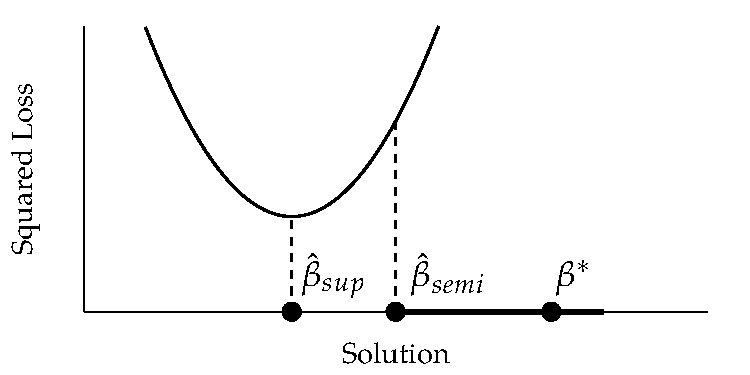
\includegraphics[width=\maxwidth]{figure/constrainedproblem-1} 

}

\caption{An example where implicitly constrained optimization improves performance. The supervised solution $\hat{\beta}_{sup}$ which minimizes the supervised loss (the solid curve), is not part of the interval of allowed solutions. The solution that minimizes this supervised loss within the allowed interval is $\hat{\beta}_{semi}$. This solution is closer to the optimal solution ${\beta}^{\ast}$ than the supervised solution $\hat{\beta}_{sup}$.}\label{fig:constrainedproblem}
\end{figure}


\end{knitrout}

Using the set of labeled data, we can construct a supervised solution $\hat{\beta}_{sup}$ that minimizes the loss on the training set of $\Nlab$ labeled objects (see Figure \ref{fig:constrainedproblem}):

\begin{equation} \label{supervisedsolution}
\hat{\beta}_{sup} = \operatorname*{argmin}_{\beta \in \mathbb{R}} \sum_{i=1}^{\Nlab} (x_i \beta - y_i)^2 \, .
\end{equation}

Now, either this solution falls within the constrained region, $\hat{\beta}_{sup} \in \Cb$ or not, $\hat{\beta}_{sup} \notin \Cb$, with different consequences:

\begin{enumerate}
  \item If $\hat{\beta}_{sup} \in \Cb$ there is a labeling of the unlabeled points that gives us the same value for $\beta$. Therefore, the solution falls within the allowed region and there is no reason to update our estimate. Therefore $\hat{\beta}_{semi}=\hat{\beta}_{sup}$.
  \item Alternatively, if $\hat{\beta}_{sup} \notin  \Cb$, the solution is outside of the constrained region (as shown in Figure \ref{fig:constrainedproblem}): there is no possible labeling of the unlabeled data that will give the same solution as $\hat{\beta}_{sup}$. We then update the $\beta$ to be the $\beta$ within the constrained region that minimizes the loss on the supervised training set. As can be seen from Figure \ref{fig:constrainedproblem}, this will be a point on the boundary of the interval. Note that $\hat{\beta}_{semi}$ is now closer to $\beta^{*}$ than $\hat{\beta}_{sup}$. Since the true loss function $R^*(\beta)$ is convex  and achieves its minimum in the optimal solution, corresponding to the true labeling, the risk of our semi-supervised solution will always be equal to or lower than the loss of the supervised solution.
\end{enumerate}

Thus, the proposed update either improves the estimate of the parameter $\beta$ or it does not change the supervised estimate. In no case will the semi-supervised solution be worse than the supervised solution, in terms of the expected squared loss. This concludes the proof of the first part of the theorem.

The last part of the theorem gives a general condition when, in expectation, our semi-supervised approach will outperform the supervised learner. Because $\hat{\beta}_{semi}$ will never be worse than $\hat{\beta}_{sup}$, to prove this we only need to show that for some observation of a labeled point with positive $f_{X,Y}(x,y)>0$, the estimated $\hat{\beta}_{sup}$ is outside of the interval $\Cb$, in which case $R^*(\hat{\beta}_{semi}) < R^*(\hat{\beta}_{sup})$. 

If we observe an object labeled $1$ with feature value $x$, the corresponding estimate $\hat{\beta}_{sup}=\tfrac{1}{x}$. Since the improvement in loss will only result if this estimate is not in the constrained region, we need to show that

\begin{equation} \label{eq:condition}
P(\tfrac{1}{x} \notin \Cb,y=1)>0 \, .
\end{equation}

To do this, consider the bounds of the interval $\Cb$. These most extreme values are obtained whenever all negative values of $x$ are assigned label $0$ while the positive $x$ get labels $1$, or the other way around. From \eqref{eqn:sslsolution} and writing $\mathbb{E}(X^2)=\int_{-\infty}^{\infty} { x^2 f_X(x) \mathrm{d}x}$ we find the interval is given by

\begin{equation} \label{eq:condition2}
\Cb=\left[ \frac{\int_{-\infty}^{0}{x f_X(x) \mathrm{d}x }}{\mathbb{E}(X^2)},\frac{\int_{0}^{\infty}{x f_X(x)  \mathrm{d}x }}{\mathbb{E}(X^2)} \right] \, .
\end{equation}
Combining this with \eqref{eq:condition}, we get the condition

\begin{equation} \label{eq:condition3}
P \left( \frac{\mathbb{E}(X^2)}{\int_{-\infty}^{0}{x f_X(x)  \mathrm{d}x }} < x < 0 \vee 0 < x < \frac{\mathbb{E}(X^2)}{\int_{0}^{\infty}{x f_X(x)  \mathrm{d}x }},y=1 \right) > 0 \, .
\end{equation}
Since $f_{X,Y}$ is assumed to be continuous, $\mathbb{E}[X^2]>0$, and the lower bound in this equation is always smaller than $0$, while the upper bound is always larger than $0$. The assumption of the continuity of $f_{X,Y}$ ensures that  \eqref{eq:condition3} holds whenever $f_{X,Y}(0,1)>0$.  The property $f_{X,Y}(0,1)>0$ is satisfied by many distributions of the data. The result, therefore, indicates, that in the case of $1$ labeled sample improvement is not only possible, but will occur in many cases. When we have multiple labeled examples, this effect will likely become smaller. This makes sense: the more labeled data we have to estimate the parameter, the smaller the impact of the unlabeled objects will be. \hfill
\end{proof}

\section{Empirical Results} 
\label{section:empiricalresults}
To study the properties of the proposed semi-supervised approach to least squares classification, we compare how this approach fares against supervised least squares classification without the constraints. 

For comparison we include two alternative semi-supervised approaches and an oracle solution: 
\paragraph{Self-Learning} Using a simple procedure proposed by \citet{McLachlan1975}, among others, the supervised least squares classifier is updated iteratively by using its class predictions on the unlabeled objects as the labels for the unlabeled objects in the next iteration. This is done until convergence.

\paragraph{Updated Second Moment Least Squares (USM)} In this approach we replace the second moment matrix $\mathbf{X}^T \mathbf{X}$ with an appropriately scaled matrix $\XeT \Xe$ similar to the estimator studied in \citep{Shaffer1991}:
$$
\boldsymbol{\hat{\beta}}_{USM} = \left( \tfrac{\Nlab}{\Nlab+\Nunl} \XeT \Xe \right)^{-1} \mathbf{X}^T \mathbf{y}
$$
where $\Xe$ and $\mathbf{y}$ are centered. This centering ensures that results do not depend on the particular encoding of the labels used. We will refer to this as updated second moment least squares (USM) classification. 

\paragraph{Oracle} The performance of the least squares classifier if all unlabeled objects were labeled as well. This serves as the unattainable upper bound on the performance of any semi-supervised learner. 


A description of the datasets used for our experiments is given in Table \ref{table:datasets-icls}. We use datasets from both the UCI repository \citep{Lichman2013} and from the benchmark datasets proposed by \citet{Chapelle2006}. While the benchmark datasets proposed in \citet{Chapelle2006} are useful, in our experience, the results on these datasets are very homogeneous because of the similarity in their dimensionality and their low Bayes errors. The UCI datasets are more diverse both in terms of the number of objects and features as well as the nature of the underlying problems. Taken together, this collection allows us to investigate the properties of our approach for a wide range of problems.
All the code used to run the experiments is available from the first author's website.

% latex table generated in R 3.2.1 by xtable 1.7-4 package
% Thu Nov 12 10:25:41 2015
\begin{table}[ht]
\centering
\caption{Description of the datasets used in the experiments. PCA99 refers to the number of principal components required to retain at least 99\% of the variance. Majority refers to the proportion of the number of objects from the largest class} 
\label{table:datasets-icls}
%\footnotesize
\begin{tabular}{lrrrrr}

  \toprule
Dataset & Objects & Features & PCA99 & Majority & Source \\ 
  \midrule
\textsc{Haberman} & 306 &   3 &   3 & 0.74 & \citep{Lichman2013} \\ 
  \textsc{Ionosphere} & 351 &  33 &  30 & 0.64 & \citep{Lichman2013} \\ 
  \textsc{Parkinsons} & 195 &  22 &  12 & 0.75 & \citep{Lichman2013} \\ 
  \textsc{Diabetes} & 768 &   8 &   8 & 0.65 & \citep{Lichman2013} \\ 
  \textsc{Sonar} & 208 &  60 &  43 & 0.53 & \citep{Lichman2013} \\ 
  \textsc{SPECT} & 267 &  22 &  21 & 0.79 & \citep{Lichman2013} \\ 
  \textsc{SPECTF} & 267 &  44 &  37 & 0.79 & \citep{Lichman2013} \\ 
  \textsc{Transfusion} & 748 &   4 &   3 & 0.76 & \citep{Lichman2013} \\ 
  \textsc{WDBC} & 569 &  30 &  17 & 0.63 & \citep{Lichman2013} \\ 
  \textsc{Mammography} & 961 &   9 &   9 & 0.54 & \citep{Lichman2013} \\ 
  \textsc{Digit1} & 1500 & 241 & 221 & 0.51 & \citep{Chapelle2006} \\ 
  \textsc{USPS} & 1500 & 241 & 183 & 0.80 & \citep{Chapelle2006} \\ 
  \textsc{COIL2} & 1500 & 241 & 114 & 0.50 & \citep{Chapelle2006} \\ 
  \textsc{BCI} & 400 & 117 &  45 & 0.50 & \citep{Chapelle2006} \\ 
  \textsc{g241c} & 1500 & 241 & 235 & 0.50 & \citep{Chapelle2006} \\ 
  \textsc{g241d} & 1500 & 241 & 235 & 0.50 & \citep{Chapelle2006} \\ 
   \bottomrule
\end{tabular}
\end{table}


\subsection{Peaking Behaviour in Semi-supervised Least Squares}
With fewer than $\featdim$ samples, the \emph{supervised} least squares classifier that utilizes a pseudo-inverse is known to exhibit a peaking phenomenon, as described by \citet{Opper1995,Raudys1998}: Starting from a single observation, expected classification errors generally decrease as we add more data before errors increase again to reach a maximum approximately when the number of features is equal to the number of observations. This phenomenon can also be observed in the semi-supervised setting. Figures~\ref{fig:peaking-icls} and \ref{fig:peakingzoom} show learning curves of the methods considered here, using $10$ labeled training objects and an increasing number of unlabeled objects. Performance is evaluated on objects that were not in the labeled or unlabeled set. The Oracle classifier indicates the mean error when we do have the labels for the unlabeled objects and therefore corresponds to the peaking phenomenon in the supervised case. In the supervised case, several proposals have been done to ameliorate this peaking behaviour, such as feature selection, regularization, removing objects, injecting noise in the features, or adding redundant features \citep{Skurichina1999}. The semi-supervised learners suffer from the same peaking phenomenon, except that unlike the Oracle, USM and ICLS do not fully recover from the initial increase in classification error.

We have no full explanation for the observed peaking behaviour in the semi-supervised setting. Even in the supervised setting the behaviour remains elusive. The two observation we do make are: 1. that the peak occurs at the same location for both the supervised and semi-supervised scenarios, which is likely due to the dependence of all methods on the inverse of $\XeT \Xe$ and 2. that the subspace defined by the input data is the defining characteristic for the location of the peak.

This peaking behaviour is not the primary topic of this work and in the remainder we will restrict our attention to the case where there are enough labeled objects such that the matrix $\mathbf{X}^T \mathbf{X}$ is invertible. 

\begin{knitrout}
\definecolor{shadecolor}{rgb}{1, 1, 1}\color{fgcolor}\begin{figure}
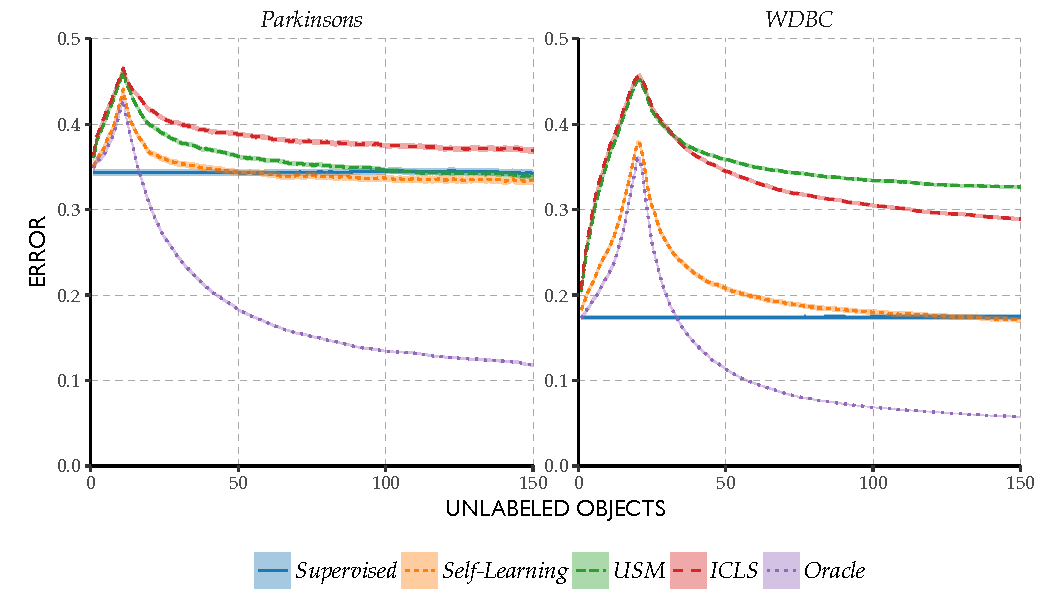
\includegraphics[width=\maxwidth]{figure/peaking-icls-1} \caption[Peaking phenomenon in Semi-supervised Least Squares Classification]{Peaking phenomenon in Semi-supervised Least Squares Classification. The lines indicate the mean classification error for $\Nlab=\max(\featdim+5,20)$ and 1000 repeats. The shaded areas indicate the standard error of the mean, which are so small in this case, they are barely perceptible.}\label{fig:peaking-icls}
\end{figure}


\end{knitrout}


\begin{knitrout}
\definecolor{shadecolor}{rgb}{1, 1, 1}\color{fgcolor}\begin{figure}
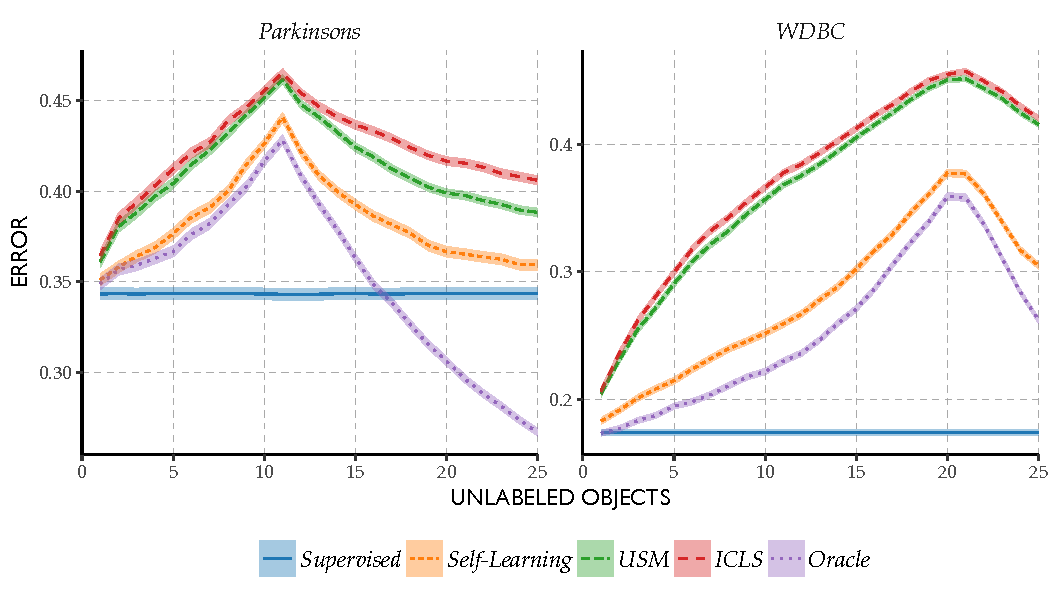
\includegraphics[width=\maxwidth]{figure/peakingzoom-1} \caption{Zoomed in version of Figure~\ref{fig:peaking-icls}}\label{fig:peakingzoom}
\end{figure}


\end{knitrout}

\subsection{Comparison of Learning Curves}
We study the behavior of the expected classification error of the ICLS procedure for different sizes of the unlabeled set. This statistic has two desired properties. First of all it should never be higher than the expected classification error of the supervised solution, which is based on only the labeled data. Secondly, the expected classification error should not increase as we add more unlabeled data. A semi-supervised classifier that has both these properties can be used safely, since adding unlabeled data and continuing to add more unlabeled data will never decrease performance, on average. 

Experiments were conducted as follows. For each dataset, $\Nlab$ labeled points were randomly chosen, where we make sure to sample at least 1 object from each of the two classes. Since the peaking phenomenon described in the previous section is not main topic of this work, we avoid this situation by considering the setting in which the labeled design matrix is of full rank, which we ensure by setting $\Nlab=\featdim+5$, the dimensionality of the dataset plus five observations. For all datasets we ensure a minimum of $\Nlab=20$ labeled objects.

Next, we create unlabeled subsets of increasing size $\Nunl=[2,4,8,...,1024]$ by randomly selecting points from the original dataset without replacement. The classifiers are trained using these subsets and the classification performance is evaluated on the remaining objects. Since the test set decreases in size as the number of unlabeled objects increases, the standard error slightly increases with the number of unlabeled objects.

The results of these experiments are shown in Figure \ref{fig:errorcurves-icls}. We report the mean classification error as well as the standard error of this mean. As can be seen from the tight confidence bands, this offers an accurate estimate of the expected classification error.

This procedure of sampling labeled and unlabeled points is repeated $1000$ times and the average classification error (Figure \ref{fig:errorcurves-icls}) and squared loss (Figure \ref{fig:losscurves}) on the test set is determined. The latter is done to evaluate whether the approach is effective in increasing generalization performance in terms of the loss used in estimating the classifier. This is the same loss that we consider in Theorem \ref{theorem:1d}. Even though in applications the ultimate goal may typically be classification performance, this allows us to study whether problems occur because of the optimization itself, or because of the link between the surrogate loss used and the classification error.

\begin{knitrout}
\definecolor{shadecolor}{rgb}{1, 1, 1}\color{fgcolor}\begin{figure}
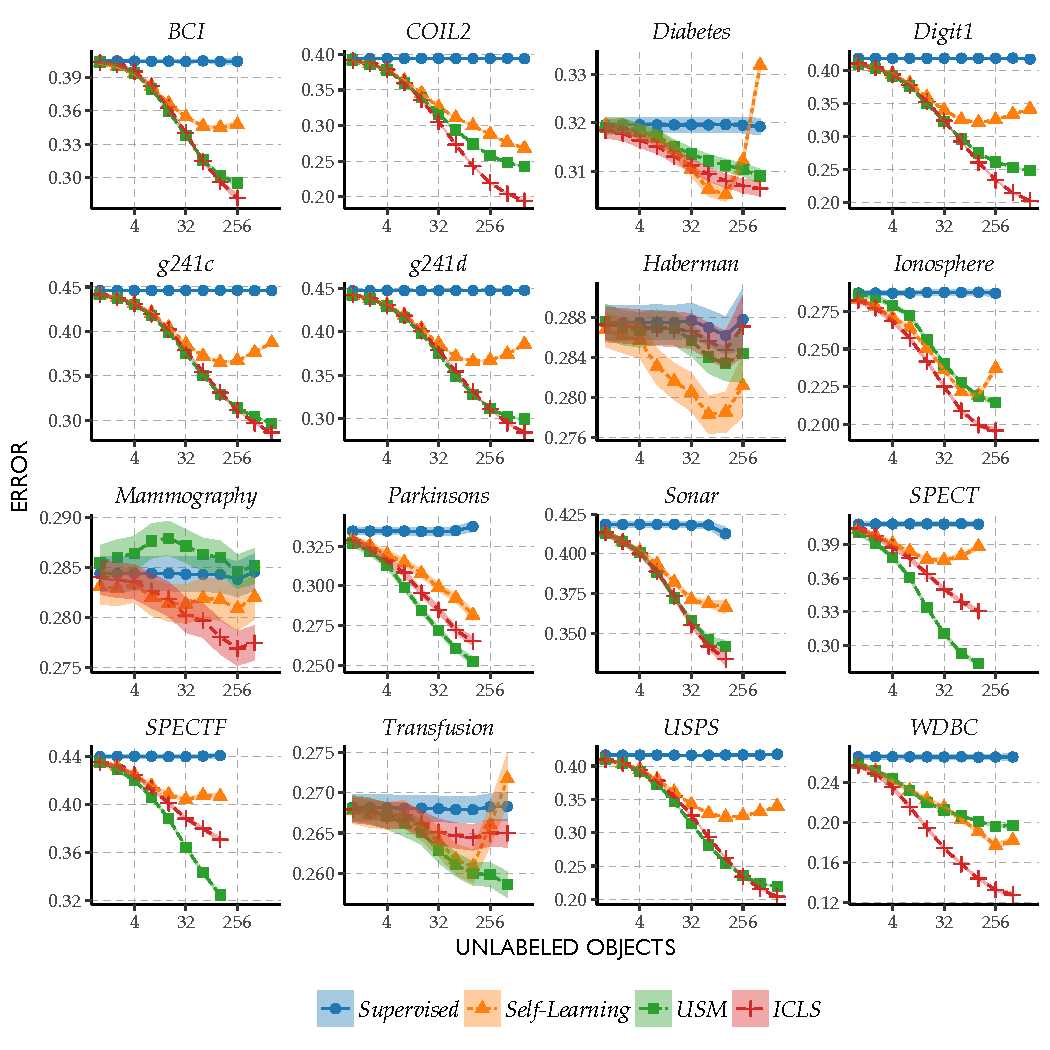
\includegraphics[width=\maxwidth]{figure/errorcurves-icls-1} \caption[Mean classification error for $\Nlab=\max(\featdim+5,20)$ and 1000 repeats]{Mean classification error for $\Nlab=\max(\featdim+5,20)$ and 1000 repeats. The shaded areas indicate  the standard error of the mean, which are so small in some cases, they are barely perceptible.}\label{fig:errorcurves-icls}
\end{figure}


\end{knitrout}


We find that, generally, the ICLS procedure has monotonically decreasing error curves as the number of unlabeled samples increases, unlike self-learning. On the \textsc{Diabetes} and \textsc{Transfusion} datasets, the performance of self-learning becomes worse than the supervised solution when more unlabeled data is added, while the ICLS classifier again exhibits a monotonic decrease of the average error rate. The USM classifier performs well on most datasets except for the \textsc{Mammography} dataset, where both in terms of average error rates and squared loss, performance is worse than the supervised classifier.

When we compare the error curves and the loss curves, the non monotonically decreasing losses for the self-learner correspond to increased errors. In general, however, similar losses for different classifiers can give rise to different behaviours in terms of error rates.

\subsection{Benchmark Performance} \label{subsection:crossvalidation}
We now consider the performance of these classifiers in a cross-validation setting. The experiment is set up as follows. For each dataset, the objects are randomly divided into $10$ folds. We iteratively go through the folds using $1$ fold as validation set, and the other $9$ as the training set. From this training set, we then randomly select $\Nlab=\max(\featdim+5,20)$ labeled objects, as in the previous experiment, and use the rest as unlabeled data. After predicting labels for the validation set for each fold, the classification error is then determined by comparing the predicted labels to the real labels. This is repeated $100$ times, while randomly assigning objects to folds in each iteration.

\begin{knitrout}
\definecolor{shadecolor}{rgb}{1, 1, 1}\color{fgcolor}\begin{figure}
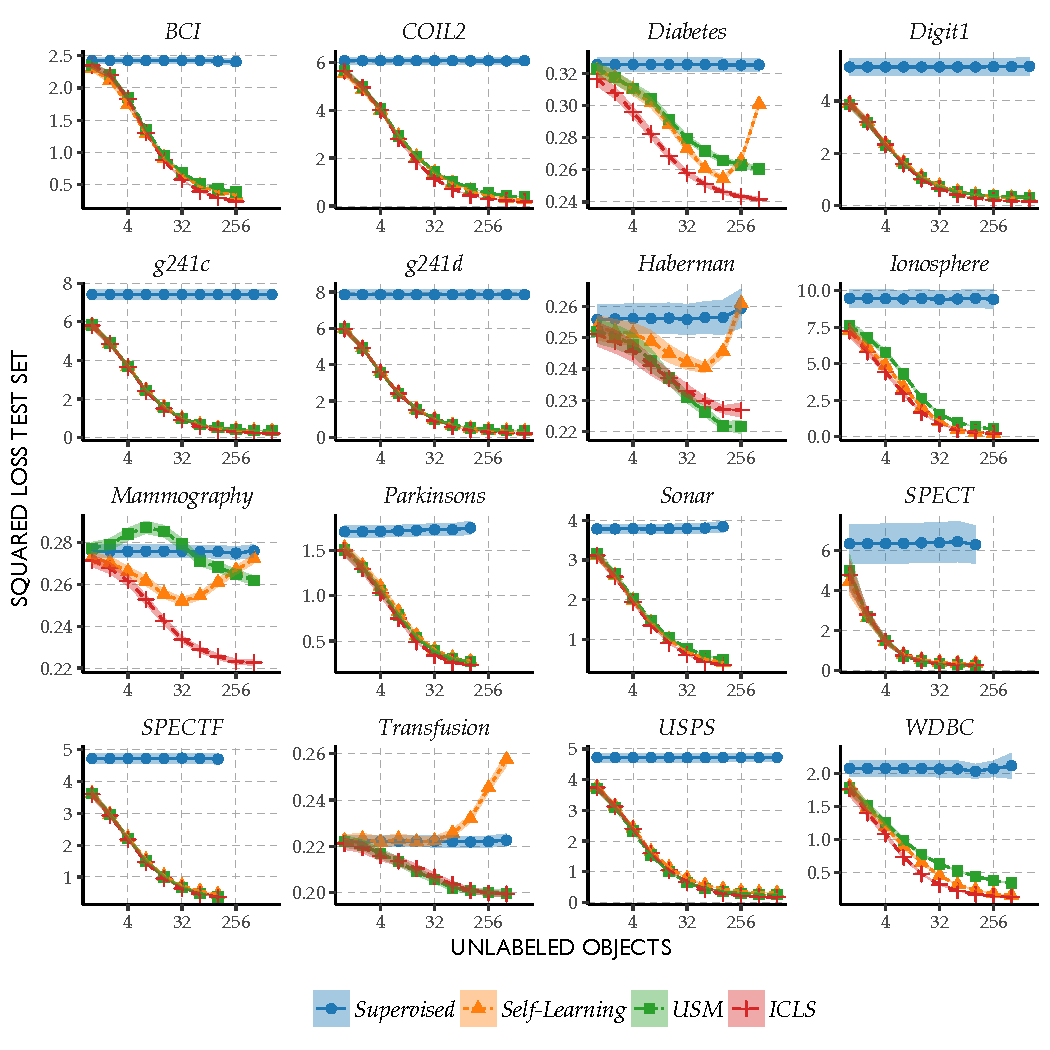
\includegraphics[width=\maxwidth]{figure/losscurves-1} \caption[Mean squared loss on the test set for $\Nlab=\max(\featdim+5,20)$ and 1000 repeats]{Mean squared loss on the test set for $\Nlab=\max(\featdim+5,20)$ and 1000 repeats. The shaded areas indicate the standard error of the mean, which are so small in some cases, they are barely perceptible.}\label{fig:losscurves}
\end{figure}


\end{knitrout}


The cross-validation procedure used here is slightly different from that described in \citep{Chapelle2006}, to make it more closely relate to the cross-validation procedure that is usually employed in supervised learning. More specifically, our procedure ensures the validation sets are independent (non-overlapping), such that, after going over all the folds, each object is in the validation set only once. This is different from the procedure in \citep{Chapelle2006}, were the authors ensure the \emph{labeled} sets are non-overlapping. We have not found a qualitative difference in the error rates, however, when using the procedure proposed in \citep{Chapelle2006}. The advantage of the procedure employed here is that every object gets a single predicted label, allowing for the direct comparison of predictions of different classifiers.

\begin{table}[t]
\caption{Results for the Least Squares Classifier. Average 10-fold cross-validation error and (between parentheses) number of times the error of the semi-supervised classifier is higher than the supervised error for 100 repeats. Indicated in \textbf{bold} is which semi-supervised classifier has lowest average error. A Wilcoxon signed rank test at 0.01 significance level is done to determine whether a semi-supervised classifier is significantly worse than the supervised classifier, indicated by \underline{underlined} values.} \label{table:cvresults}
\centering
\begin{tabular}{llllll}
  \toprule
% latex table generated in R 3.4.1 by xtable 1.8-2 package
% Wed Nov  8 16:47:40 2017
Dataset & Supervised & Self-Learning & USM & ICLS & Oracle \\ 
  \midrule
\textsc{Haberman} & 0.29 & \textbf{0.28 (33)} & 0.28 (42) & 0.29 (24) & 0.26 (11) \\ 
  \textsc{Ionosphere} & 0.29 & 0.24 (1) & 0.22 (1) & \textbf{0.19 (0)} & 0.13 (0) \\ 
  \textsc{Parkinsons} & 0.34 & 0.29 (5) & \textbf{0.25 (3)} & 0.26 (1) & 0.12 (0) \\ 
  \textsc{Diabetes} & 0.32 & \underline{0.34 (83)} & 0.31 (31) & \textbf{0.31 (7)} & 0.23 (0) \\ 
  \textsc{Sonar} & 0.42 & 0.37 (5) & 0.34 (3) & \textbf{0.33 (1)} & 0.25 (0) \\ 
  \textsc{SPECT} & 0.41 & 0.39 (28) & \textbf{0.28 (0)} & 0.33 (1) & 0.18 (0) \\ 
  \textsc{SPECTF} & 0.43 & 0.40 (14) & \textbf{0.31 (0)} & 0.36 (2) & 0.23 (0) \\ 
  \textsc{Transfusion} & 0.27 & \underline{0.28 (63)} & \textbf{0.26 (30)} & 0.27 (25) & 0.23 (2) \\ 
  \textsc{WDBC} & 0.27 & 0.18 (0) & 0.20 (2) & \textbf{0.13 (0)} & 0.04 (0) \\ 
  \textsc{Mammography} & 0.28 & 0.28 (28) & 0.28 (54) & \textbf{0.27 (14)} & 0.20 (0) \\ 
  \textsc{Digit1} & 0.42 & 0.34 (0) & 0.25 (0) & \textbf{0.20 (0)} & 0.06 (0) \\ 
  \textsc{USPS} & 0.42 & 0.34 (0) & 0.22 (0) & \textbf{0.20 (0)} & 0.09 (0) \\ 
  \textsc{COIL2} & 0.39 & 0.27 (0) & 0.24 (0) & \textbf{0.19 (0)} & 0.10 (0) \\ 
  \textsc{BCI} & 0.41 & 0.35 (1) & 0.30 (0) & \textbf{0.28 (0)} & 0.16 (0) \\ 
  \textsc{g241c} & 0.45 & 0.39 (0) & 0.30 (0) & \textbf{0.29 (0)} & 0.14 (0) \\ 
  \textsc{g241d} & 0.45 & 0.39 (0) & 0.30 (0) & \textbf{0.29 (0)} & 0.13 (0) \\ 
   \bottomrule

\end{tabular}
\end{table}



The results shown in Table \ref{table:cvresults} tell a similar story to those in the previous experiment. Most importantly for the purposes of this paper, ICLS, in general, offers solutions that give at least no higher expected classification error than the supervised procedure. 
On many of these datasets, the self-learning approach seems to share this property. However, if we look at for how many of the cross-validation repeats the ICLS and self-learning give lower error than the supervised solution, there is a clear difference. The self-learning solution gives a higher error on more of the repeats than ICLS, for all of the datasets.

The results also show that unlabeled information is of use. Particularly on the last six datasets, ICLS and USM offers large improvement in classification accuracy over the supervised solution. The differences in performance between ICLS and self-learning can also be quite substantial, where ICLS outperforms self-learning on most of the datasets.
USM performs well on many of the datasets, especially when we consider how simple and computationally efficient this procedure is. 

\begin{table}[t]
\caption{Results for the Support Vector Classifier. Average 10-fold cross-validation error and (between parentheses) number of times the error of the semi-supervised classifier is higher than the supervised error for 100 repeats. Indicated in \textbf{bold} is which semi-supervised classifier has lowest average error. A Wilcoxon signed rank test at 0.01 significance level is done to determine whether a semi-supervised classifier is significantly worse than the supervised classifier, indicated by \underline{underlined} values.} \label{table:cvresults-svm}
\centering
\begin{tabular}{llllll}
\toprule
% latex table generated in R 3.4.1 by xtable 1.8-2 package
% Wed Nov  8 16:47:41 2017
Dataset & Supervised & Self-Learning & TSVM & Oracle \\ 
  \midrule
\textsc{Haberman} & 0.29 & \textbf{0.29 (34)} & \underline{0.32 (92)} & 0.26 (8) \\ 
  \textsc{Ionosphere} & 0.17 & \underline{0.18 (81)} & 0.17 (51) & 0.11 (0) \\ 
  \textsc{Parkinsons} & 0.22 & \textbf{0.22 (32)} & 0.22 (60) & 0.14 (0) \\ 
  \textsc{Diabetes} & 0.31 & 0.31 (40) & \textbf{0.28 (7)} & 0.23 (0) \\ 
  \textsc{Sonar} & 0.26 & 0.26 (53) & \textbf{0.25 (33)} & 0.25 (25) \\ 
  \textsc{SPECT} & 0.30 & 0.28 (13) & \textbf{0.25 (3)} & 0.18 (0) \\ 
  \textsc{SPECTF} & 0.30 & 0.29 (28) & \textbf{0.28 (29)} & 0.21 (0) \\ 
  \textsc{Transfusion} & 0.27 & 0.27 (59) & \underline{0.29 (96)} & 0.23 (0) \\ 
  \textsc{WDBC} & 0.06 & 0.06 (53) & \textbf{0.05 (30)} & 0.03 (0) \\ 
  \textsc{Mammography} & 0.27 & 0.28 (60) & \textbf{0.25 (3)} & 0.20 (0) \\ 
  \textsc{Digit1} & 0.08 & \underline{0.08 (85)} & \textbf{0.06 (1)} & 0.05 (0) \\ 
  \textsc{USPS} & 0.14 & 0.13 (17) & \textbf{0.12 (5)} & 0.11 (1) \\ 
  \textsc{COIL2} & 0.16 & \underline{0.16 (75)} & \underline{0.19 (100)} & 0.09 (0) \\ 
  \textsc{BCI} & 0.28 & \underline{0.29 (70)} & \underline{0.36 (99)} & 0.17 (0) \\ 
  \textsc{g241c} & 0.22 & \underline{0.23 (87)} & \textbf{0.17 (0)} & 0.16 (0) \\ 
  \textsc{g241d} & 0.23 & \underline{0.24 (90)} & \textbf{0.17 (0)} & 0.16 (0) \\ 
   \bottomrule


\end{tabular}
\end{table}

While we are interested in a semi-supervised procedure that outperforms the supervised least squares classifier, for comparison we repeated the experiment for the (linear) supervised SVM, self-learning applied to the SVM and the Transductive SVM. We used the SVM and TSVM implementations of \citet{Sindhwani2006},  setting the $L_2$ regularization parameter to $\lambda=1$ and the influence parameter of the unlabeled data to $1$, as was also done in \citep{Sindhwani2006}. The experiment is set up in the same way as the one in Table \ref{table:cvresults}. The results are shown in Table~\ref{table:cvresults-svm}.

On many of the datasets, the supervised support vector classifier has a lower error than the supervised least squares classifier, due to the use of a regularization term in the SVM implementation, which we do not include in our analysis and which makes the results difficult to compare directly to the results in Table~\ref{table:cvresults}. Self-learning performs worse compared to the least squares setting, which may be a consequence of the supervised solution already being a decent solution on some of these datasets. The Transductive SVM offers some improvements over the supervised solution. Compared to ICLS, however, the TSVM gives worse performance than the supervised solution on many more datasets and many more repeats, the exact behaviour we attempted to avoid when constructing ICLS.

\section{Discussion}
\subsection*{From Theory to Empirical Results}
The results presented in this paper are rather promising, especially in the light of the negative theoretical performance results presented in the literature \citep{Cozman2006}. The result in Theorem \ref{theorem:1d}, to start with, indicates the proposed procedure is in some way robust against reduction in performance. The strong result of this theorem, stating that performance never gets worse, holds in the 1D case with unlimited unlabeled data and no intercept in the model. A slightly weaker result, that performance does not degrade on average may still hold without these assumptions. This last statement is corroborated by the empirical results showing improvements in averaged squared errors for ICLS throughout.

The results in the previous section also indicate that such improved results hold in terms of the misclassification error, at least on this collection of datasets. These empirical observations are encouraging because we are often interested in misclassification error and not the squared loss that was considered in Theorem \ref{theorem:1d}. Furthermore the experiments were carried out in the multivariate setting with an intercept term using limited unlabeled data, rather than the unlimited unlabeled data setting considered in the theorem. This indicates that minimizing the supervised loss over the subset $\Cb$, leads to a semi-supervised learner with desirable behavior, both theoretically in terms of risk and empirically in terms of classification error.

\subsection*{Robustness}
The method considered in this work is different from most previous work in semi-supervised learning in that it is inherently robust against a decrease in performance. 
The robustness of the method comes from the fact that we do not accept solutions that do not work on the labeled data. The goal of semi-supervised learning is to improve supervised techniques using the additional information inherent in the additional unlabeled objects. Previous approaches have done this by changing the loss function that is being optimized, in particular by introducing an extra term corresponding to assumptions about the unlabeled data. The loss function then becomes a mixture between the supervised objective and an unsupervised objective, which may lead to decreased performance as we observed in Table~\ref{table:cvresults-svm}. If the goal is classification, we propose that the loss function should remain the supervised loss function. The unlabeled objects are merely used to introduce constraints on the possible solutions to this loss function, but do not change its functional form.

\subsection*{Assumptions}
Most other semi-supervised techniques rely on introducing useful assumptions that link information about the distribution of the features $P_X$ to the posterior of the classes $P_{Y|X}$. It has been argued that, for discriminative classifiers, semi-supervised learning is impossible without these additional assumptions about the link between labeled and unlabeled objects \citep{Seeger2001,Singh2008}. ICLS, however, is both a discriminative classifier and no explicit additional assumptions about this link are made.  Any assumptions that are present follow, implicitly, from the choice of squared loss as the loss function and from the chosen hypothesis space.

In fact, additional assumptions may actually be at the root of the problem: clearly if such an additional assumption is correct, a semi-supervised classifier can gain from it, but if the assumption is incorrect, degraded performance may ensue.  What we leverage in our approach are the implicit assumptions that are, in a sense, intrinsic to the supervised least squares classifier. 

One could argue that constraining the solutions to $\Cb$ is an assumption as well. It corresponds to a very weak assumption about the supervised classifier: that it will improve when we add additional labeled data. This is generally assumed in the supervised setting as well. The lack of additional assumptions has another advantage: no additional hyperparameter value needs to be selected that controls the importance of the unlabeled data for the results in Sections \ref{section:theoreticalresults} and \ref{section:empiricalresults} to hold as ICLS acts as a type of data dependent regularization.

Note that the solution provided by self-learning is, by construction, also in the constrained subset $\Cb$. The difference with ICLS is that in ICLS the choice of estimate from $\Cb$ is based on information of the labeled objects only, while self-learning also uses the imputed labels on the unlabeled objects. This may lead to self-deception: if the imputed labels are wrong, a good fit for these wrongly imputed labels does not necessarily lead to an improved $\boldsymbol{\beta}$. In fact, it might lead to worse choices as shown in the results.

\subsection*{Time Complexity}
In terms of the number of features, ICLS scales in the same way as the supervised least squares solution, where the main bottleneck is the calculation of $(\XeT \Xe)^{-1}$. Furthermore, the quadratic programming formulation of ICLS presented in Section \ref{section:method} allows one to use the standard and constantly improving tools from convex optimization to find the ICLS estimate. Unfortunately one has to go from a convex problem with $\featdim+1$ variables in the supervised case to a constrained convex problem with $\Nunl$ variables for ICLS. For very large $\Nunl$, this may not currently be computationally feasible. Further insight in the general nature of the semi-supervised solutions that one obtains can lead to more dedicated and potentially better scalable methods to solve the quadratic programming problem we have to deal with in our approach.

Compared to ICLS, self-learning seems more favorable in terms of computational cost. Self-learning usually converges in a few iterations, where each iteration has at most the cost of one supervised least squares estimation. In our implementations, however, self-learning and ICLS had similar training times (Figure \ref{fig:timecurves}). USM with its simple closed form solution has much lower training times and performs surprisingly well.


\begin{knitrout}
\definecolor{shadecolor}{rgb}{1, 1, 1}\color{fgcolor}\begin{figure}
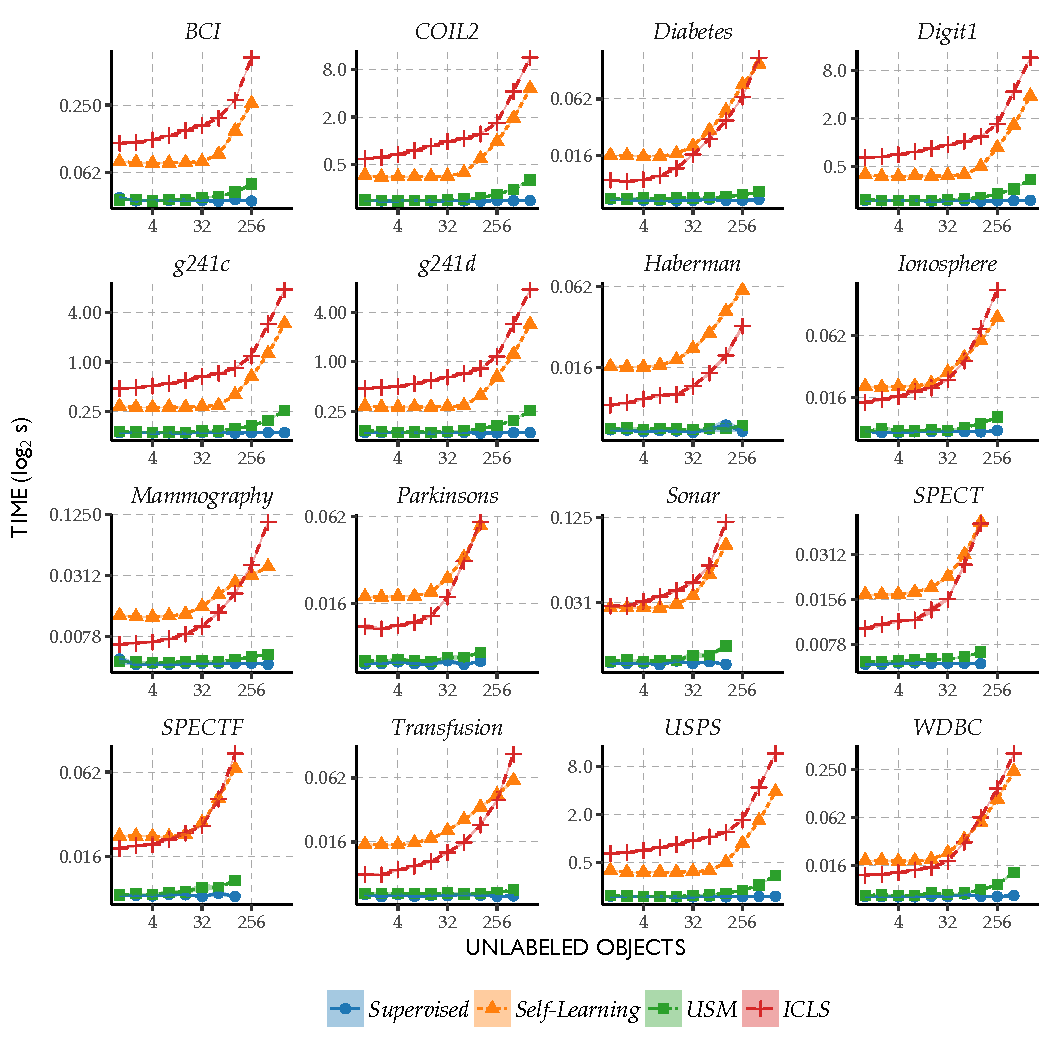
\includegraphics[width=\maxwidth]{figure/timecurves-1} \caption[Average Training Time for 1000 repeats]{Average Training Time for 1000 repeats. The shaded areas indicate the standard error of the mean.}\label{fig:timecurves}
\end{figure}


\end{knitrout}

\subsection*{Squared Loss}
Generally, models used in practice do not directly minimize misclassification error. For computational reasons, often convex surrogate losses, such as the one employed here are minimized. It is therefore interesting to look at the performance of a classifier in terms of these surrogate losses \citep{Loog2016a}. We have chosen to restrict ourselves to a particular convex loss and attempted to ensure improvement in terms of this chosen loss function.

When we compare the average squared loss on the test set, ICLS, USM and self-learning often seem to offer similar performance. This is quite unlike the results in, for instance \citep{Loog2010,Loog2014b}, where the self-learner often performed much worse in terms of the loss than an approach based on constraining the solution using unlabeled data. While \citet{Loog2010,Loog2014b} consider a generative classifier, we consider a discriminative classifier, in which case self-learning may be less susceptible to increases in the loss. Self-learning does, however, still increase the loss on some datasets, unlike ICLS.

The peaking phenomenon described in \citep{Opper1995,Raudys1998} is known to occur for squared loss minimization when we increase the number of labeled samples. Here we find it also occurs when we change the number of unlabeled samples. It seems that ICLS and USM are more sensitive to this problem than self-learning. As yet, we do not have any explanation for this behavior. Further improvements to the current approach may start by trying to understand this occurrence of peaking.

\subsection*{Other Losses}
While the results presented in this work are promising for squared loss, an open question is what other classifiers could benefit from the implicitly constrained approach considered here. Using negative log likelihood as a loss function, for instance, also leads to an interesting implicitly constrained semi-supervised classifier, for instance, in linear discriminant analysis \citep{Krijthe2014}. 

In the derivation of ICLS, we made use of the closed-form solution given an imputed labeling to derive a quadratic programming problem in terms of the labels. For many loss functions, closed-form solutions do not exist, which prohibits a straightforward formulation of their implicitly constrained semi-supervised counterparts. Without a supervised closed-form solution one cannot straightaway apply techniques like gradient descent to the parameters as this typically leads to solutions that are outside of the set $\Cb$, even if the loss considered is differentiable.

\subsection*{More Constraints}
In Figure \ref{fig:constrainedsubset}, we illustrate that projecting onto the subset $\Cb$ causes improvement as long as a better solution $\hat{\beta}_{oracle}$ than the supervised solution is within $\Cb$. A smaller $\Cb$ will give a larger improvement, since the semi-supervised solution is going to be closer to $\hat{\beta}_{oracle}$. In the extreme case where only $\hat{\beta}_{oracle}$ forms the subset, this clearly gives a large improvement over supervised learning. It therefore makes sense to think about reducing the size of $\Cb$. In the approach presented in this work, however, to ensure a better solution $\hat{\beta}_{oracle}$ than the supervised solution is always within the constraint set with probability $P(\hat{\beta}_{oracle} \in \Cb)=1$, our choice of $\Cb$ is conservatively large. It contains elements corresponding to all labelings of the unlabeled points, even extremely unlikely ones. 

By excluding unlikely labelings from the subset, the size of $\Cb$ may shrink, while the probability that it includes $\hat{\beta}_{oracle}$ remains high. For instance, one might exclude labelings with class priors that are very unlikely to occur, given the class priors that are observed in the labeled data, a strategy which is also employed in Transductive SVMs where it is necessary for it to converge to meaningful local optima. Changes to $\Cb$ may, therefore, allow for larger improvements in terms of the risk or classification error, while introducing a small chance of deterioration in performance.

\section{Conclusion}
This work introduced a new semi-supervised approach to least squares classification. By implicitly considering all possible labelings of the unlabeled objects and choosing the one that minimizes the loss on the labeled observations, we derived a robust classifier with a simple quadratic programming formulation. For this procedure, in the univariate setting with a linear model without intercept, we can prove it never degrades performance in terms of squared loss (Theorem 1). Experimental results indicate that in expectation this robustness also holds in terms of classification error on real datasets. Hence, semi-supervised learning for least squares classification without additional assumptions can lead to improvements over supervised least squares classification both in theory and in practice.

\chapter[Implicitly Constrained Semi-supervised Linear Discriminant Analysis]{Implicitly Constrained Semi-supervised\\Linear Discriminant Analysis}
\chaptermark{Implicitly Constrained LDA}
\label{chapter:iclda}
\blfootnote{This chapter appeared as: Krijthe, J.H. \& Loog, M., 2014. Implicitly Constrained Semi-Supervised Linear Discriminant Analysis. In Proceedings of the 22nd International Conference on Pattern Recognition (pp. 3762–3767).}


\begin{abstract}
Semi-supervised learning is an important and active topic of research in pattern recognition. For classification using linear discriminant analysis specifically, several semi-supervised variants have been proposed. Using any one of these methods is not guaranteed to outperform the supervised classifier which does not take the additional unlabeled data into account. In this work we compare traditional Expectation Maximization type approaches for semi-supervised linear discriminant analysis with approaches based on intrinsic constraints and propose a new principled approach for semi-supervised linear discriminant analysis, using so-called implicit constraints. We explore the relationships between these methods and consider the question if and in what sense we can expect improvement in performance over the supervised procedure. The constraint based approaches are more robust to misspecification of the model, and may outperform alternatives that make more assumptions on the data in terms of the log-likelihood of unseen objects.
\end{abstract}

\section{Introduction}
In many real-world pattern recognition tasks, obtaining labeled examples to train classification algorithms is much more expensive than obtaining unlabeled examples. These tasks include document and image classification \cite{Nigam2000} where unlabeled objects can easily be downloaded from the web, part of speech tagging \cite{Elworthy1994}, protein function prediction \cite{Weston2005} and many others. Using unlabeled data to improve the training of a classification procedure, however, requires semi-supervised variants of supervised classifiers to make use of this additional unlabeled data. Research into semi-supervised learning has therefore seen an increasing amount of interest in the last decade \cite{Chapelle2006}.

In supervised learning adding additional labeled training data improves performance for most classification routines. This does not generally hold for semi-supervised learning \cite{Cozman2006}. Adding additional unlabeled data may actually deteriorate classification performance. This can happen when the underlying assumptions of the model do not hold. In effect, disregarding the unlabeled data can lead to a better solution.

In this work we consider linear discriminant analysis (LDA) applied to classification. Several semi-supervised adaptations of this supervised procedure have been proposed. These approaches may suffer from the problem that additional unlabeled data degrade performance. To counter this problem, \cite{Loog2014a} introduced moment constrained LDA, which offers a more robust type of semi-supervised LDA. The recently introduced idea of implicitly constrained estimation \cite{Krijthe2015}, is another method that relies on constraints given by the unlabeled data. We compare these two approaches to other semi-supervised methods, in particular, expectation maximization and self-learning, and empirically study in what sense we can expect improvement by employing any of these semi-supervised methods.

The contributions of this work are the following:

\begin{itemize}
  \item Introduce a new, principled approach to semi-supervised LDA: implicitly constrained LDA
  \item Offer a comparison of semi-supervised versions of linear discriminant analysis
  \item Explore ways in which we can expect these semi-supervised methods to offer improvements over the supervised variant, in particular in terms of the log likelihood
\end{itemize}

The rest of this paper is organized as follows. After discussing related work, we introduce several approaches to semi-supervised linear discriminant analysis. These methods are then compared on an illustrative toy problem and in an empirical study using several benchmark datasets. We end with a discussion of the results and conclude.

\section{Related Work}
Some of the earliest work on semi-supervised learning was done by \cite{McLachlan1975,McLachlan1977} who studied the self-learning approach applied to linear discriminant analysis. This has later also been referred to as Yarowsky's algorithm \cite{Yarowsky1995}. This approach is closely related to Expectation Maximization \cite{Abney2004}, where, in a generative model, the unknown labels are integrated out of the likelihood function and the resulting marginal likelihood is maximized \cite{Dempster1977}. More recent work on discriminative semi-supervised learning has focussed on introducing assumptions that relate unlabeled data to the labeled objects \cite{Chapelle2006}. These assumptions usually take the form of either a manifold assumption \cite{Zhu2003}, encoding that labels change smoothly in a low dimensional manifold, or a low-density class separation assumption used in, for instance, transductive support vector machines \cite{Bennett1998,Joachims1999} and entropy regularization \cite{Grandvalet2005}. 

Work on semi-supervised LDA has tried to incorporate unlabeled data by leveraging the increase in accuracy of estimators of quantities that do not rely on labels. An approach relying on the more accurate estimate of the total covariance matrix of both labeled and unlabeled objects is taken for dimensionality reduction in Normalized LDA, proposed by \cite{Fan2008} and similar work by \cite{Cai2007}. In addition to this covariance matrix, \cite{Loog2014a} also include the more accurate estimate of the overal mean of the data and propose two solutions to solve a subsequent optimization problem. Building on these results, in \cite{Krijthe2015} we introduced implicitly constrained least squares classification, a semi-supervised adaptation of least squares classification. Since this procedure proved both theoretically and practically successful for a discriminative classifier, here we consider whether the idea of implicitly constrained semi-supervised learning can be extended to generative classifiers such as LDA.

\section{Methods}
We will first introduce linear discriminant analysis as a supervised classification algorithm and discuss different semi-supervised procedures. We will consider 2-class classification problems, where we are given an $N_l \times d$ design matrix $\mathbf{X}$, where $N_l$ is the number of labeled objects and $d$ is the number of features. For these observations we are given a label vector $\mathbf{y}=\{0,1\}^{N_l}$. Additionally, in the semi-supervised setting we have an $N_u \times d$ design matrix $\mathbf{X}_\textrm{u}$ without a corresponding $\mathbf{y}_\textrm{u}$ for the unlabeled observations.

\subsection{Supervised LDA}
In supervised linear discriminant analysis, we model the 2 classes as having multivariate normal distributions with the same covariance matrix $\boldsymbol{\Sigma}$ and differing means $\boldsymbol{\mu}_1$ and $\boldsymbol{\mu}_2$. To estimate the parameters of this model, we maximize the likelihood, or, equivalently, the log likelihood function:
\begin{align}
\label{eq:lda}
L(\theta|\mathbf{X},\mathbf{y})= \sum_{i=1}^{N_l} & y_i \log(\pi_1 \mathcal{N}(\mathbf{x}_i|\boldsymbol{\mu}_1,\mathbf{\Sigma})) \nonumber \\
& +(1-y_i) \log(\pi_2 \mathcal{N}(\mathbf{x}_i|\boldsymbol{\mu}_2,\mathbf{\Sigma})) \,,
\end{align}
% L() \sum_{i=1}^{N_l} (y_i\left(log(\pi_1) -\frac{1}{2} log(2 \pi) -log(|\Sigma_1|) - (x_i - \mu_1)' \Sigma^{-1} (x_i - \mu_1) \right)\\ 
% + y_i\left(log(\pi_2) -\frac{1}{2} log(2 \pi) -log(|\Sigma_1|) - (x_i - \mu_2)' \Sigma^{-1} (x_i - \mu_2) \right)
where $\theta=\left( \pi_1,\pi_2, \boldsymbol{\mu}_1,\boldsymbol{\mu}_2,\mathbf{\Sigma} \right)$, $\mathcal{N}(\mathbf{x}_i|\boldsymbol{\mu},\mathbf{\Sigma})$ denotes the density of a multivariate normal distribution with mean $\boldsymbol{\mu}$ and covariance $\mathbf{\Sigma}$ evaluated at $\mathbf{x}_i$ and $\pi_c$ denotes the prior probability for class $c$. The closed form solution to this maximization is given by the estimators:
\begin{align}
\label{eq:ldasolution}
\hat{\pi}_1 &= \frac{\sum_{i=1}^{N_l} y_i}{N_l}, \hspace{20pt} \hat{\pi}_2 = \frac{\sum_{i=1}^{N_l} (1-y_i)}{N_l}  \nonumber \\
\hat{\boldsymbol{\mu}}_1 &= \frac{\sum_{i=1}^{N_l} y_i \mathbf{x}_i}{\sum_{i=1}^{N_l} y_i}, \hspace{20pt} \hat{\boldsymbol{\mu}}_2 = \frac{\sum_{i=1}^{N_l} (1-y_i) \mathbf{x}_i}{\sum_{i=1}^{N_l} (1-y_i)}  \nonumber  \\
\hat{\mathbf{\Sigma}} &= \frac{1}{N_l} \sum_{i=1}^{N_l} y_i (\mathbf{x}_i-\boldsymbol{\mu}_1) (\mathbf{x}_i-\boldsymbol{\mu}_1)^\top  \nonumber \\
& \hspace{20pt} + (1-y_i) (\mathbf{x}_i-\boldsymbol{\mu}_2) (\mathbf{x}_i-\boldsymbol{\mu}_2)^\top 
\end{align}
Here the maximum likelihood estimator $\hat{\mathbf{\Sigma}}$ is a biased estimator for the covariance matrix. Given a set of labeled objects $(\mathbf{X},\mathbf{y})$, we can estimate these parameters and find the posterior for a new object $\mathbf{x}$ using:
\begin{equation}
p(c=1|\mathbf{x})=\frac{\pi_1 \mathcal{N}(\mathbf{x}|\hat{\boldsymbol{\mu}}_1,\hat{\mathbf{\Sigma}})}{\sum_{c=1}^{2} \pi_c \mathcal{N}(\mathbf{x}|\hat{\boldsymbol{\mu}}_c,\hat{\mathbf{\Sigma}})} \,.
\end{equation}
This posterior distribution can be employed for classification by assigning objects to the class for which its posterior is highest. We now consider several adaptations of this classification procedure to the  semi-supervised setting.

\subsection{Self-Learning LDA (SLLDA)}
A common and straightforward adaptation of any supervised learning algorithm to the semi-supervised setting is self-learning, which is also known as Yarowsky's algorithm or bootstrapping \cite{McLachlan1975,Yarowsky1995}. Starting out with a classifier trained on the labeled data only, labels are  predicted for the unlabeled objects. These objects, with their imputed labels are then used in the next iteration to retrain the classifier. This new classifier is now used to relabel the unlabeled objects. This is done until the predicted labels on the unlabeled objects converge. \citet{Abney2004} studies the underlying loss that this procedure minimizes and proves its convergence.

\subsection{Expectation Maximization LDA (EMLDA)}
Assuming the mixture model of Equation \eqref{eq:lda} and treating the unobserved labels $\mathbf{y}_\textrm{u}$ as latent variables, a possible adaptation of this model is to add a term for the unlabeled data to the objective function and to integrate out the unknown labels, $\mathbf{y}_\textrm{u}$, to find the marginal likelihood:
\begin{align}
l(\theta|\mathbf{X},\mathbf{y},\mathbf{X}_\textrm{u})=\prod_{i=1}^{N_l}\left(\pi_1 \mathcal{N}(\mathbf{x}_i|\boldsymbol{\mu}_1,\mathbf{\Sigma})\right)^{y_i} \left(\pi_2 \mathcal{N}(\mathbf{x}_i|\boldsymbol{\mu}_2,\mathbf{\Sigma})\right)^{1-y_i}  \nonumber \\ 
\times \prod_{i=1}^{N_u} \sum_{c=1}^2 \pi_c \mathcal{N}(\mathbf{x}_i|\boldsymbol{\mu}_c,\Sigma) \,.
\end{align}
Maximizing this marginal likelihood, or equivalently, the log of this function, is harder than the supervised objective in Equation \eqref{eq:lda}, since the expression contains a log over a sum. However, we can solve this optimization problem using the well-known expectation maximization (EM) algorithm \cite{Dempster1977, Nigam2000}. In EM, the log over the sum is bounded from below through Jensen's inequality. In the M step of the algorithm, we maximize this bound by updating the parameters using the imputed labels obtained in the E step. In practice, the M step consists of the same update as in Equation \eqref{eq:ldasolution}, where the sum is no longer over the labeled objects but also the unlabeled objects using the imputed posteriors, or responsibilities, from the E step. In the E step the lower bound is made tight by updating the imputed labels using the posterior under the new parameter estimates. This is done until convergence. 
In effect this procedure is very similar to self-learning, where instead of hard labels, a probability over labelings is used. Both self-learning and EM suffer from the problem of wrongly imputed labels that can reinforce their wrongly imputed values because the parameters are updated as if they were the true labels.

\subsection{Moment Constrained LDA (MCLDA)}
An alternative to the EM-like approaches like EMLDA and SLLDA was proposed by \citet{Loog2010} in the form of moment constrained parameter estimation. The main idea is that there are certain constraints that link parameters that are calculated using feature values alone, with parameters which require the labels. In the case of LDA \cite{Loog2014a}, for instance, the overal mean of the data is linked to the means of the two classes through:
\begin{equation}
\label{eq:constraintmean}
\boldsymbol{\mu}_t=\pi_1 \boldsymbol{\mu}_1 + \pi_2 \boldsymbol{\mu}_2
\end{equation}
Were $\boldsymbol{\mu}_t$ is the overal mean on all the data and therefore does not depend on the labels.
The total covariance matrix $\mathbf{\Sigma}_t$ is linked to the within-class covariance matrix $\mathbf{\Sigma}$ and between-class covariance matrix $\mathbf{\Sigma}_b$, the covariance matrix of the means. Only the latter two rely on the labels:
\begin{equation}
\label{eq:constraintcovariance}
\mathbf{\Sigma}_t=\mathbf{\Sigma} + \mathbf{\Sigma}_b
\end{equation}
Recognizing that the unlabeled data allow us to more accurately estimate the parameters in these constraints that do not rely on the labels, \citet{Loog2014a} points out that this more accurate estimate will generally violate the constraints, meaning the other label-dependent estimates should be updated accordingly.

An ad hoc way to update the parameters based on these more accurate estimates \cite{Loog2014a} leads to the following updated moment constrained estimators:
\begin{align}
\hat{\boldsymbol{\mu}}_c^{MC} & =\hat{\mathbf{\Theta}}^{\frac{1}{2}} \hat{\mathbf{\Sigma}}_t^{-\frac{1}{2}} (\hat{\boldsymbol{\mu}}_c - \sum_{j=1}^{2} \hat{\pi}_j \hat{\boldsymbol{\mu}}_j ) + \hat{\boldsymbol{\mu}} \\
\hat{\mathbf{\Sigma}}^{MC} &= \hat{\mathbf{\Theta}}^{\frac{1}{2}} \hat{\mathbf{\Sigma}}_t^{-\frac{1}{2}} \hat{\mathbf{\Sigma}} \hat{\mathbf{\Sigma}}_t^{-\frac{1}{2}} \hat{\mathbf{\Theta}}^{\frac{1}{2}}
\end{align}
where $\hat{\boldsymbol{\mu}}$ and $\hat{\mathbf{\Theta}}$ are the overal mean and overal covariance estimated on all labeled and unlabeled data, while $\hat{\mathbf{\Sigma}}_t$ is the overal covariance estimated on the labeled data alone.

Alternatively and slightly more formally, \citet{Loog2012b} force the constraints to be satisfied by maximizing the likelihood on the labeled objects under the constraints in Equations \eqref{eq:constraintmean} and \eqref{eq:constraintcovariance}. This leads to a non-convex objective function that can be solved numerically. In this work we use the simpler ad hoc constraints.

\subsection{Implicitly Constrained LDA (ICLDA)}
The former approach requires the identification of specific constraints. Ideally, we would like these constraints to emerge implicitly from a choice of supervised learner and a given set of unlabeled objects. Implicitly constrained semi-supervised learning attempts to do just that. The underlying intuition is that if we could enumerate all possible $2^{N_u}$ labelings, and train the corresponding classifiers, the classifier based on the true but unknown labels is in this set. This classifier would generally outperform the supervised classifier. Two problems arise:

\begin{enumerate}
\item How do we find a classifier in this set that is close to the one based on the true but unknown labels?
\item How do we efficiently traverse this enormous set of possible labelings without having to enumerate them all?
\end{enumerate}
As for the first problem: a safe way to know how well a solution performs in terms of our supervised objective is to estimate its performance using the labeled objects. We therefore propose the following objective:

\begin{equation}
\label{eq:iclda}
\operatorname*{arg\,max}_{\left( \pi_1,\pi_2, \boldsymbol{\mu}_1,\boldsymbol{\mu}_2,\mathbf{\Sigma}\right) \in \mathcal{C}_\theta} L(\pi_1,\pi_2, \boldsymbol{\mu}_1,\boldsymbol{\mu}_2,\mathbf{\Sigma}|\mathbf{X},\mathbf{y}) \,,
\end{equation}
where
\begin{align}
\mathcal{C}_{\boldsymbol{\theta}} = \left\{ \operatorname*{arg\,max} L(\pi_1,\pi_2, \boldsymbol{\mu}_1,\boldsymbol{\mu}_2,\mathbf{\Sigma}| \mathbf{X}_\textrm{e}, \mathbf{y}_\textrm{e}) : \mathbf{y}_\textrm{u} \in [0,1]^{N_u} \right\} \,, \nonumber
\end{align}
and $\mathbf{X}_\textrm{e}=[\mathbf{X}^\top \mathbf{X}_\textrm{u}^\top]^\top, \mathbf{y}_\textrm{e}=[\mathbf{y}^\top \mathbf{y}_\textrm{u}^\top]^\top$ are the design matrix and class vector extended with the unlabeled data. This can be interpreted as optimizing the same objective function as supervised LDA, with the additional constraint that the solution has to be attainable by a particular assignment of responsibilities (partial assignments to classes) for the unlabeled objects.

As for the second problem: since, for a given imputed labeling, we have a closed form solution for the parameters, the gradient of the supervised loss \eqref{eq:iclda} with respect to the responsibilities $\mathbf{y}_\textrm{u}$ can be found using
\begin{equation}
\frac{\partial L(\theta|\mathbf{X},\mathbf{y})}{\partial \mathbf{y}_\textrm{u}} = \frac{\partial L(\theta|\mathbf{X},\mathbf{y})}{\partial \theta} \frac{\partial \phi(\mathbf{y}_\textrm{u})}{\partial \mathbf{y}_\textrm{u}} 
\end{equation}
where $\phi(\mathbf{y}_\textrm{u})=\theta$ is the function that has as input a particular labeling of the points, and outputs the parameters $\theta=\left(\pi_1,\pi_2, \boldsymbol{\mu}_1,\boldsymbol{\mu}_2,\mathbf{\Sigma}\right)$, similar to Equation \eqref{eq:ldasolution}.

This can be used to efficiently move through the set of solutions using a simple gradient ascent procedure that takes into account the $[0,1]$ bounds on the responsibilities.

\begin{knitrout}
\definecolor{shadecolor}{rgb}{1, 1, 1}\color{fgcolor}\begin{figure}
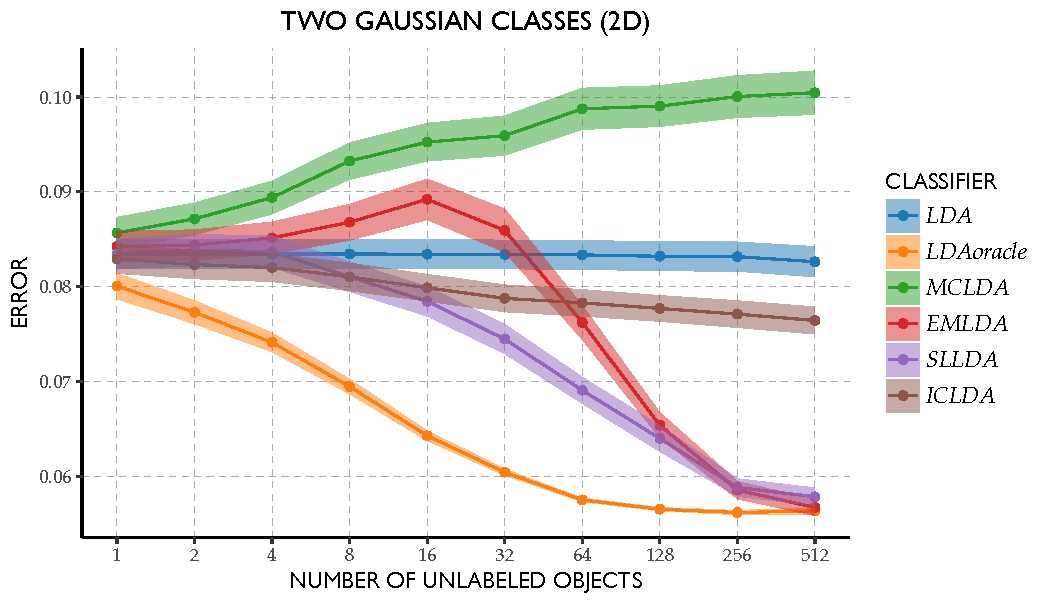
\includegraphics[width=\maxwidth]{figure/learningcurvegauss-1} \caption[Semi-supervised learning curve on the Gaussian data set using 500 repeats]{Semi-supervised learning curve on the Gaussian data set using 500 repeats. The shaded regions indicate one standard error around the mean. Since their assumptions hold exactly, SLLDA and EMLDA work very well. ICLDA also outperforms the supervised LDA.}\label{fig:learningcurvegauss}
\end{figure}


\end{knitrout}

\section{Experimental setup and results}
We present simulations on an illustrative toy dataset and a set of benchmark datasets. Other than the classifiers covered in the previous section, we also include the LDA classifier trained using all labels of the unlabeled data (LDAoracle) as an upper bound on the performance of any semi-supervised procedure. The experiments can be reproduced using code from the authors' website. 

\subsection{Toy Problems}
To illustrate the behaviour of ICLDA when compared to EMLDA we consider two toy datasets. In both cases we have two multivariate normal distributions centered at respectively $\boldsymbol{\mu}_1=[1,1]^\top$ and $\boldsymbol{\mu}_2=[-1,-1]^\top$ and equal covariance $\mathbf{\Sigma}=0.6 \mathbf{I}$, with $\mathbf{I}$ the $2 \times 2$ identity matrix. An example is given in Figure \ref{fig:toyplots}. In the right column, these two gaussians correspond to the different classes. In the left column, we consider the case where the decision boundary is actually perpendicular to the boundary in the other setting. This means that the right column corresponds exactly to the assumptions of EM, while this is not the case in the left column. Figure \ref{fig:toyplots} illustrates what happens in a particular sample from this problem were we draw $10$ labeled and $990$ unlabeled objects. When the assumption does not hold, EMLDA forces the decision boundary to fall between the two gaussian clusters leading to a much worse solution than the supervised LDA based on only a few labeled examples. The ICLDA solution does not deviate from the correct boundary by much. When the assumptions do hold, EMLDA finds the correct boundary, as expected, while ICLDA only does minor adjustments in this case. 

While one could claim that ICLDA is more robust, one could also expect ICLDA to never lead to any improvements. Figure \ref{fig:learningcurvegauss} shows the results when resampling from the data distribution in the second example and shows that ICLDA does lead to improvement on average in the second dataset, while not making the mistake in the first dataset where the LDA assumptions do not hold.

\begin{knitrout}
\definecolor{shadecolor}{rgb}{1, 1, 1}\color{fgcolor}\begin{figure}
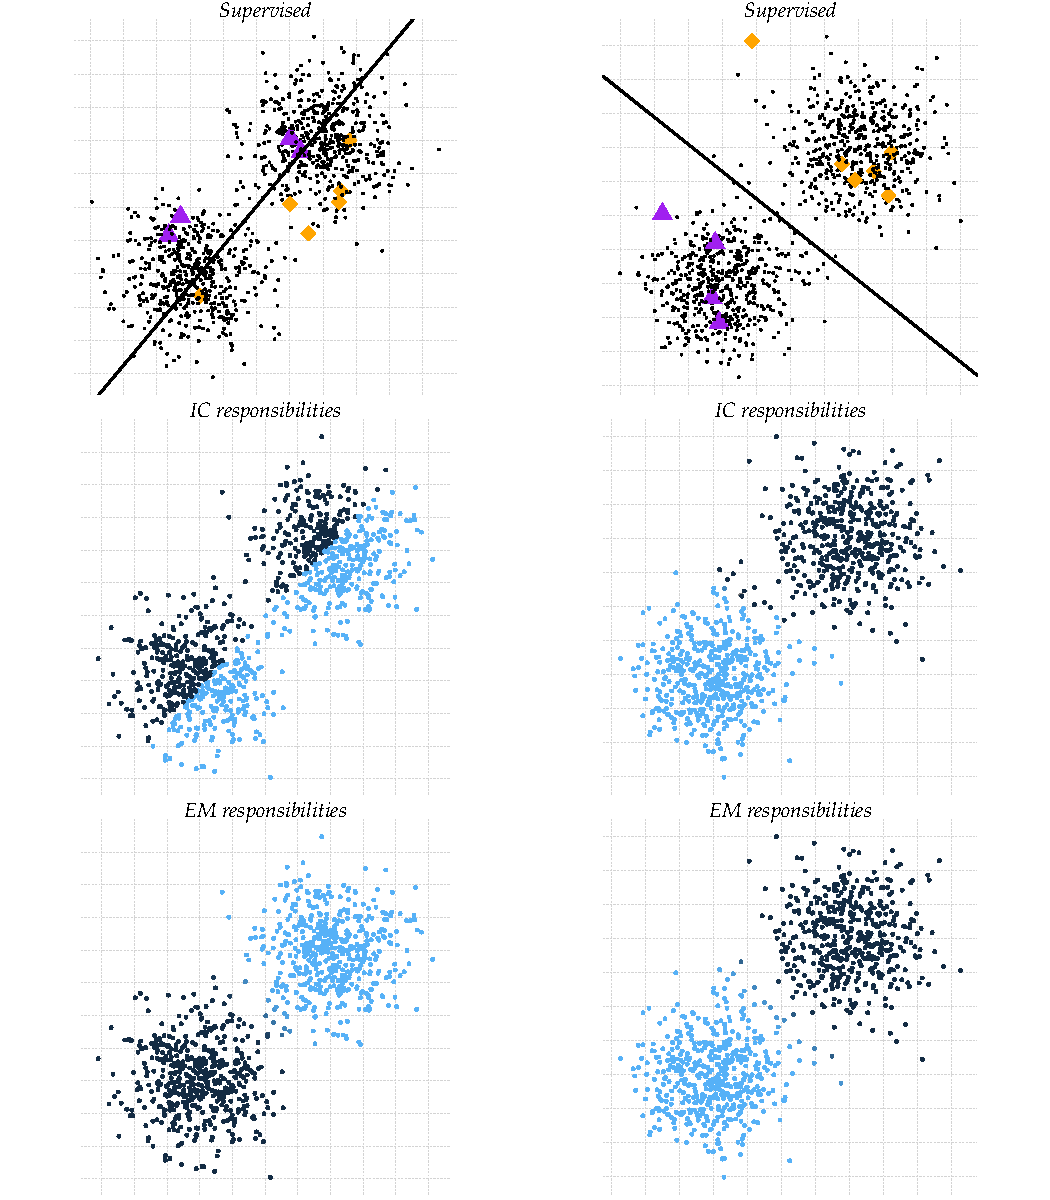
\includegraphics[width=\maxwidth]{figure/toyplots-1} \caption[Behaviour on the two-class two dimensional gaussian datasets, with 10 labeled objects and 990 unlabeled objects]{Behaviour on the two-class two dimensional gaussian datasets, with 10 labeled objects and 990 unlabeled objects. The first column shows the scatterplot and the trained responsibilities for respectively ICLDA and EMLDA on a dataset where the decision boundary does not adhere to the assumptions of EMLDA. The second column shows the results when the decision boundary is in between the two Gaussian classes. The black line indicates the decision boundary of a supervised learner trained using only the labeled data. Note that in the first column, the responsibilities of EM are very different from the true labels, while IC is not as sensitive to this problem.}\label{fig:toyplots}
\end{figure}


\end{knitrout}


\subsection{Simulations on Benchmark Datasets}
We test the behaviour of the considered procedures using datasets from the UCI machine learning repository \cite{Lichman2013}, as well as from \cite{Chapelle2006}. Their characteristics can be found in Table \ref{table:datasets}.

\begin{table}[!t]
\caption{Description of the datasets used in the experiments}
\label{table:datasets}
\centering
\begin{tabular}{llll}
  \toprule
 Name & Objects & Features & Source \\ 
  \midrule
  \textsc{Haberman} & 305 &   4 & \cite{Lichman2013} \\ 
  \textsc{Ionosphere} & 351 &  33 & \cite{Lichman2013} \\ 
  \textsc{Parkinsons} & 195 &  20 & \cite{Lichman2013} \\ 
  \textsc{Pima} & 768 &   9 & \cite{Lichman2013} \\ 
  \textsc{Sonar} & 208 &  61 & \cite{Lichman2013} \\ 
  \textsc{SPECT} & 265 &  23 & \cite{Lichman2013} \\ 
  \textsc{SPECTF} & 265 &  45 & \cite{Lichman2013} \\ 
  \textsc{Transfusion} & 748 &   4 & \cite{Lichman2013} \\ 
  \textsc{WDBC} & 568 &  30 & \cite{Lichman2013} \\
  \textsc{BCI} & 400 & 118 & \cite{Chapelle2006} \\ 
   \bottomrule
\end{tabular}
\end{table}

A cross-validation experiment was carried out as follows. Each of the datasets were split into $10$ folds. Every fold was used as a validation set once, while the other nine folds were used for training. The data in these nine folds was randomly split into a labeled and an unlabeled part, where the labeled part had $\max(2d,10)$ objects, while the rest was used as unlabeled objects. This procedure was repeated $20$ times and the average error and average negative log likelihood (the loss function of LDA) on the test set was determined. The results can be found in Tables \ref{table:cvresults-error} and \ref{table:cvresults-loss}.

To study the behaviour of these classifiers for differing amount of unlabeled data, we estimated semi-supervised learning curves by randomly drawing $\max(2d,10)$ labeled objects from the datasets, and using an increasing randomly chosen set as unlabeled data. The remaining objects formed the test set. This procedure was repeated 500 times and the average and standard error of the classification error and negative log likelihood were determined. The learning curves for 3 datasets can be found in Figure \ref{fig:errorcurves}.

\begin{table*}
\caption{Average 10-fold cross-validation error and its standard deviation over 20 repeats. Indicated in \textbf{bold} is whether a semi-supervised classifier significantly outperform the supervised LDA classifier, as measured using a t-test with a 0.05 significance level. \underline{Underlined} indicates whether a semi-supervised classifier is (significantly) best among the four semi-supervised classifiers considered.} \label{table:cvresults-error}
\centering
\footnotesize\begin{tabular}{lllllll}
\toprule
Dataset & LDA & LDAoracle & MCLDA & EMLDA & SLLDA & ICLDA \\ 
\midrule
\textsc{ Haberman }& $0.37 \pm 0.04$& $0.25 \pm 0.00$& $0.36 \pm 0.03$& $0.47 \pm 0.08$& $0.36 \pm 0.04$& $0.37 \pm 0.04$\\ 
\textsc{ Ionosphere }& $0.21 \pm 0.02$& $0.15 \pm 0.01$& $\mathbf{\underline{0.18 \pm 0.02}} $& $0.57 \pm 0.04$& $0.20 \pm 0.02$& $\mathbf{0.18 \pm 0.01} $\\ 
\textsc{ Parkinsons }& $0.27 \pm 0.03$& $0.15 \pm 0.01$& $\mathbf{\underline{0.22 \pm 0.03}} $& $0.41 \pm 0.05$& $0.26 \pm 0.03$& $\mathbf{0.23 \pm 0.03} $\\ 
\textsc{ Pima }& $0.34 \pm 0.03$& $0.23 \pm 0.00$& $\mathbf{0.32 \pm 0.02} $& $0.37 \pm 0.03$& $0.35 \pm 0.02$& $\mathbf{\underline{0.31 \pm 0.02}} $\\ 
\textsc{ Sonar }& $0.29 \pm 0.02$& $0.26 \pm 0.02$& $0.28 \pm 0.02$& $0.35 \pm 0.02$& $0.29 \pm 0.02$& $0.28 \pm 0.02$\\ 
\textsc{ SPECT }& $0.31 \pm 0.03$& $0.18 \pm 0.01$& $\mathbf{\underline{0.25 \pm 0.02}} $& $0.62 \pm 0.03$& $0.33 \pm 0.03$& $0.30 \pm 0.03$\\ 
\textsc{ SPECTF }& $0.32 \pm 0.03$& $0.24 \pm 0.01$& $\mathbf{\underline{0.28 \pm 0.03}} $& $\mathbf{0.28 \pm 0.05} $& $0.34 \pm 0.03$& $0.33 \pm 0.03$\\ 
\textsc{ Transfusion }& $0.34 \pm 0.03$& $0.23 \pm 0.00$& $\mathbf{\underline{0.32 \pm 0.03}} $& $0.52 \pm 0.09$& $0.37 \pm 0.05$& $0.33 \pm 0.03$\\ 
\textsc{ WDBC }& $0.11 \pm 0.01$& $0.04 \pm 0.00$& $\mathbf{0.09 \pm 0.01} $& $0.38 \pm 0.05$& $\mathbf{0.09 \pm 0.01} $& $\mathbf{\underline{0.08 \pm 0.01}} $\\ 
\textsc{ BCI }& $0.21 \pm 0.01$& $0.16 \pm 0.01$& $\mathbf{\underline{0.20 \pm 0.01}} $& $0.21 \pm 0.02$& $0.21 \pm 0.02$& $\mathbf{0.20 \pm 0.01} $\\ 
\bottomrule
\end{tabular}
\end{table*}



\begin{table*}
\caption{Average 10-fold cross-validation negative log-likelihood (loss) and its standard deviation over 20 repeats. Indicated in \textbf{bold} is whether a semi-supervised classifier significantly outperform the supervised LDA classifier, as measured using a t-test with a 0.05 significance level. \underline{Underlined} indicates whether a semi-supervised classifier is (significantly) best among the four semi-supervised classifiers considered. } \label{table:cvresults-loss}
\centering
\tiny\begin{tabular}{lllllll}
\toprule
Dataset & LDA & LDAoracle & MCLDA & EMLDA & SLLDA & ICLDA \\ 
\midrule
\textsc{ Haberman }& $15.88 \pm 4.37$& $10.37 \pm 0.02$& $\mathbf{11.66 \pm 2.45} $& $\mathbf{12.02 \pm 0.35} $& $\mathbf{12.08 \pm 0.20} $& $\mathbf{\underline{10.89 \pm 0.16}} $\\ 
\textsc{ Ionosphere }& $199.58 \pm 29.66$& $21.38 \pm 0.34$& $\mathbf{25.93 \pm 1.44} $& $\mathbf{22.55 \pm 0.40} $& $\mathbf{22.80 \pm 0.40} $& $\mathbf{\underline{22.22 \pm 0.33}} $\\ 
\textsc{ Parkinsons }& $-40.76 \pm 11.11$& $-71.87 \pm 0.32$& $\mathbf{-71.05 \pm 0.40} $& $\mathbf{-71.12 \pm 0.40} $& $\mathbf{-71.03 \pm 0.38} $& $\mathbf{\underline{-71.44 \pm 0.31}} $\\ 
\textsc{ Pima }& $41.98 \pm 2.99$& $29.88 \pm 0.02$& $\mathbf{31.74 \pm 0.99} $& $\mathbf{31.95 \pm 0.35} $& $\mathbf{32.07 \pm 0.36} $& $\mathbf{\underline{30.50 \pm 0.13}} $\\ 
\textsc{ Sonar }& $-59.86 \pm 1.08$& $-83.05 \pm 0.59$& $\mathbf{-82.23 \pm 0.57} $& $\mathbf{-82.85 \pm 0.55} $& $\mathbf{-82.20 \pm 0.60} $& $\mathbf{-82.58 \pm 0.57} $\\ 
\textsc{ SPECT }& $27.65 \pm 1.89$& $10.74 \pm 0.09$& $\mathbf{11.30 \pm 0.17} $& $\mathbf{12.63 \pm 0.18} $& $\mathbf{11.84 \pm 0.20} $& $\mathbf{\underline{11.19 \pm 0.13}} $\\ 
\textsc{ SPECTF }& $178.42 \pm 2.48$& $148.13 \pm 0.68$& $\mathbf{148.78 \pm 0.69} $& $\mathbf{148.44 \pm 0.69} $& $\mathbf{149.18 \pm 0.72} $& $\mathbf{148.67 \pm 0.71} $\\ 
\textsc{ Transfusion }& $17.00 \pm 2.61$& $11.48 \pm 0.02$& $\mathbf{12.23 \pm 0.54} $& $16.27 \pm 0.53$& $\mathbf{14.21 \pm 0.47} $& $\mathbf{\underline{11.88 \pm 0.17}} $\\ 
\textsc{ WDBC }& $33.15 \pm 15.14$& $-28.06 \pm 1.29$& $\mathbf{-26.73 \pm 1.23} $& $\mathbf{-26.67 \pm 1.32} $& $\mathbf{-27.78 \pm 1.28} $& $\mathbf{\underline{-27.86 \pm 1.28}} $\\ 
\textsc{ BCI }& $6.99 \pm 1.04$& $-21.04 \pm 0.41$& $\mathbf{-20.38 \pm 0.40} $& $\mathbf{-20.39 \pm 0.46} $& $\mathbf{-20.44 \pm 0.45} $& $\mathbf{\underline{-20.74 \pm 0.41}} $\\ 
\bottomrule
\end{tabular}
\end{table*}


\begin{knitrout}
\definecolor{shadecolor}{rgb}{1, 1, 1}\color{fgcolor}\begin{figure}
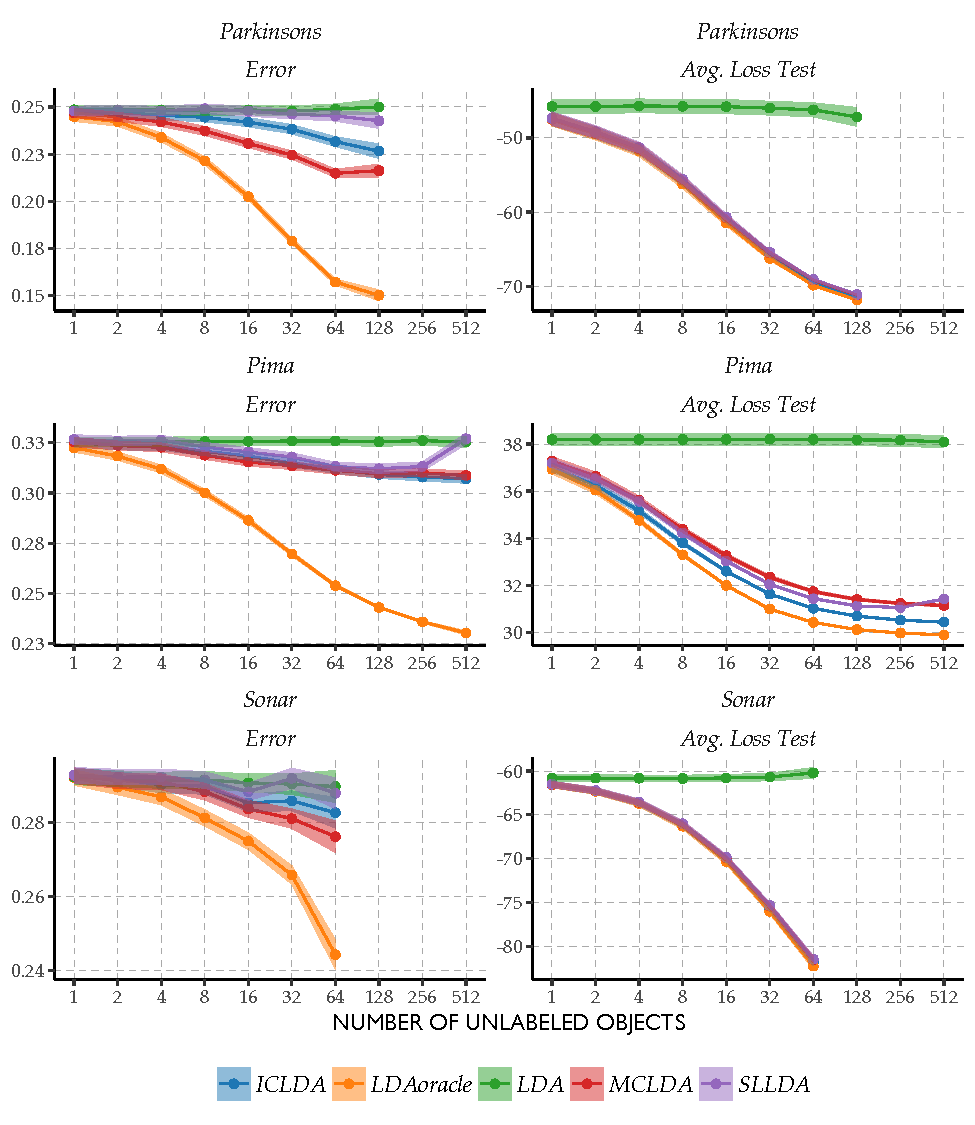
\includegraphics[width=\maxwidth]{figure/errorcurves-1} \caption[Learning curves for increasing amounts of unlabeled data for the error rate as well as the loss (negative log likelihood) for three datasets using 500 repeats]{Learning curves for increasing amounts of unlabeled data for the error rate as well as the loss (negative log likelihood) for three datasets using 500 repeats. The shaded regions indicate one standard error around the mean.}\label{fig:errorcurves}
\end{figure}


\end{knitrout}

We find that overal in terms of error rates (Table \ref{table:cvresults-error}), MCLDA seems to perform best, being both more robust than the EM approaches as well as effective in using the unlabeled information in improving error rates. While ICLDA is robust and has the best performance on 2 of the datasets, it is conservative in that it does not show improvements in terms of the classification error for many datasets where the other classifiers do offer improvements.

The picture is markedly different when we consider the log likelihood criterion that supervised LDA optimizes, evaluated on the test set (Table \ref{table:cvresults-loss}). Here ICLDA outperforms all other methods on the majority of the datasets. 

\section{Discussion}
The results show that ICLDA provides the safest semi-supervised option among the approaches to LDA that we considered. At least in terms of the log-likelihood, it provides the best performance by far. A particularly interesting observation is that the implicit constraints, in many a case, seem to add a lot to the constraints that MCLDA enforces, as also the latter classifier is consistently outperformed by ICLDA in terms of the log likelihoods achieved on the test set. As yet, we have no full understanding in what way the implicit constraints add restrictions beyond the moment constraints, apart from the fact that the former are stricter than the latter.  A deeper insight into this issue might cast further light on the workings of ICLDA.

While it is the safest version, ICLDA may be \emph{too} safe, in that it does not attain performance improvement in terms of classification error in many cases where MCLDA or the EM approaches do offer improvements. In terms of the loss on the test set, however, ICLDA is the best performing method. Since this is the objective minimized by supervised LDA as well, perhaps this is the best we could hope for in a true semi-supervised adaptation of LDA. We found similar empirical and theoretical performance results in terms of improvements in the loss on the test set when applying the implicitly constrained framework to the least squares classifier \cite{Krijthe2015}. How then, this improvement in ``surrogate'' loss relates to the eventual goal of classification error, is unclear, especially for a non-margin based loss function such as the negative log likelihood \cite{Bartlett2006}. However, since ICLDA does offer the best behaviour of supervised LDA's loss on the test set, ICLDA could be considered a step towards a principled semi-supervised version of LDA.

An open question regarding the objective function associated with ICLDA is to what extent it is convex. The solution in terms of the responsibility vector $\mathbf{y}_\textrm{u}$ is non-unique: different labelings of the points can lead to the same parameters. In terms of the parameters, however, the optimization seems to converge to a unique global optimum. While we do not have a formal proof of this, as in the case of implicitly constrained least squares classification, we conjecture that the objective function is convex in the parameters, at least in the case in which we choose to parameterize LDA by means of its canonical parameters \cite{Lehmann1998}.  In this case, LDA does lead to a convex optimization problem.

We find that the behaviour of EMLDA is more erratic than that of SLLDA. The hard label assignments could have a regularizing effect on the semi-supervised solutions, making self-learning a good and fast alternative to EM. Note that safer versions of SLLDA and EMLDA could be obtained by introducing a weight parameter to control the influence of the unlabeled data \cite{McLachlan1975}. In the limited labeled data setting, it is hard to correctly set this parameter. While this may help when dealing with larger sample sizes, the constraint approaches bring us closer to methods that always perform at least as well as their supervised counterpart. 

\section{Conclusion}
ICLDA is a principled and robust adaptation of LDA to the semi-supervised setting. In terms of error rates, it may be overly conservative. When measured in terms of the loss on the test set, however, it outperforms other semi-supervised methods. It therefore seems that there are opportunities for robust semi-supervised learners, although the performance criterion that we should consider may not be the error rate, but rather the loss that the supervised learner minimizes \cite{Loog2014b}.

  
  \chapter[Projected Estimators for Robust Semi-supervised Classification]{Projected Estimators for\\Robust Semi-supervised Classification}
\chaptermark{Projected Estimators}
\label{chapter:projection}
\blfootnote{This is chapter appeared as: Krijthe, J. H., \& Loog, M., 2017. Projected estimators for robust semi-supervised classification. Machine Learning, 106(7), pp. 993–1008. Springer}


\begin{abstract}
For semi-supervised techniques to be applied safely in practice we at least want methods to outperform their supervised counterparts. We study this question for classification using the well-known quadratic surrogate loss function. Unlike other approaches to semi-supervised learning, the procedure proposed in this work does not rely on assumptions that are not intrinsic to the classifier at hand. Using a projection of the supervised estimate onto a set of constraints imposed by the unlabeled data, we find we can safely improve over the supervised solution in terms of this quadratic loss. More specifically, we prove that, measured on the labeled and unlabeled training data, this semi-supervised procedure never gives a lower quadratic loss than the supervised alternative. To our knowledge this is the first approach that offers such strong, albeit conservative, guarantees for improvement over the supervised solution. The characteristics of our approach are explicated using benchmark datasets to further understand the similarities and differences between the quadratic loss criterion used in the theoretical results and the classification accuracy typically considered in practice.
\end{abstract}

\section{Introduction}
\label{Introduction}
We consider the problem of semi-supervised classification using the quadratic loss function, which is also known as least squares classification or Fisher's linear discriminant classification \citep{Hastie2009,Poggio2003}. Suppose we are given an $N_l \times d$ matrix with feature vectors $\vec{X}$, labels $\vec{y} \in \{0,1\}^{N_l}$ and an $N_u \times d$  matrix with unlabeled objects $\vec{X}_\text{u}$ from the same distribution as the labeled objects. The goal of semi-supervised learning is to improve the classification decision function $f: \mathbb{R}^d \to \mathbb{R}$ using the unlabeled information in $\vec{X}_\text{u}$ as compared to the case where we do not have these unlabeled objects. In this work, we focus on linear classifiers where $f(\vec{x})=\vec{w}^\top \vec{x}$. 

Much work has been done on semi-supervised classification, in particular on what additional assumptions about the unlabeled data may help improve classification performance. These additional assumptions, while successful in some settings, are less successful in others where they do not hold. In effect they can greatly deteriorate performance when compared to a supervised alternative \citep{Cozman2006}. Since, in semi-supervised applications, the number of labeled objects may be small, the effect of these assumptions is often untestable. In this work, we introduce a conservative approach to training a semi-supervised version of the least squares classifier that is guaranteed to improve over the supervised least squares classifier, in terms of the quadratic loss on the labeled and unlabeled examples. It is the first procedure for which it is possible to give strong guarantees of non-degradation of this type (Theorem~\ref{th:robustness}).

To guarantee these improvements, we avoid additional assumptions altogether. We introduce a constraint set of parameter vectors induced by the unlabeled data, which does not rely on additional assumptions about the data. Using a projection of the supervised solution vector onto this constraint set, we derive a method that can be proven to never degrade the surrogate loss evaluated on the labeled and unlabeled training data when compared to the supervised solution. Experimental results indicate that it not only never degrades, but often improves performance. Our experiments also indicate the results hold when performance is evaluated on objects in a test set that were not used as unlabeled objects during training.

The main contribution of this work is to prove that a semi-supervised learner that is guaranteed to outperform its supervised counterpart exists for some classifier. We do this by constructing one in the least squares classifier. This non-degradation property is important in practical applications, since one would like to be sure that the effort of the collection of, and computation with unlabeled data does not have an adverse effect. Our work is a conceptual step towards such methods. The goal of this work is to prove and illustrate this property.

Others have attempted to mitigate the problem of reduction in performance in semi-supervised learning by introducing safe versions of semi-supervised learners \citep{Li2011,Loog2010,Loog2014a}. These procedures do not offer any guarantees or only do so once particular assumptions about the data hold. Moreover, unlike some previous approaches, the proposed method can be formulated as a convex quadratic programming problem which can be solved using a simple gradient descent procedure.

The rest of this work is organized as follows. The next section discusses related work. Section \ref{section:projections} introduces our projection approach to semi-supervised learning. Section \ref{section:theory} discusses the theoretical performance guarantee and its implications. Section \ref{section:interpretations} provides some alternative interpretations of the method and relations to other approaches. In Section \ref{section:empirical} empirical illustrations on benchmark datasets are presented to understand how the theoretical results in terms of quadratic loss in Section \ref{section:theory} relate to classification error on an unseen test set. We end with a discussion of the results and conclude.

\section{Prior Work and Assumptions}

Early work on semi-supervised learning dealt with the missing labels through the use of Expectation Maximization in generative models or closely related self-learning \citep{McLachlan1975}. Self-learning is a simple wrapper method around any supervised procedure. Starting with a supervised learner trained only on the labeled objects, we predict labels for the unlabeled objects. Using the known labels and the predicted labels for the unlabeled objects, or potentially the predicted labels with highest confidence, we retrain the supervised learner. This process is iterated until the predicted labels converge. Although simple, this procedure has seen some practical success \citep{Nigam2000}.

\citet{Singh2008}, among others, have argued that unlabeled data can \emph{only} help if $P(\vec{x})$ and $P(y|\vec{x})$ are somehow linked. They show that when a specific cluster assumption holds, semi-supervised learning can be expected to outperform a supervised learner. The goal of our work is to show that in some cases (i.e. the least squares classifier) we do not need explicit assumptions about those links for semi-supervised learning to be possible. Instead, we leverage implicit assumptions, including possible model misspecification, that are already present in the supervised classifier. Similar to \citet{Singh2008}, we also study the finite sample case.

Most recent work on semi-supervised methods considers what assumptions about this link between $P(\vec{x})$ and $P(y|\vec{x})$ allows for the effective use of unlabeled data. A lot of work involves either the assumption that the decision boundary is in a low-density region of the feature space, or that the data is concentrated on a low-dimensional manifold. A well-known procedure using the first assumption is the Transductive SVM \citep{Joachims1999}. It can be interpreted as minimizing the following objective:
\begin{multline}
\label{eq:TSVM}
\min_{\vec{w} \in \mathbb{R}^d,\vec{y}_\text{u} \in \{-1,+1\}^{N_u}} \sum_{i=1}^{N_l} \max(1-y_i \vec{w}^\top \vec{x}_i,0) + \lambda ||\vec{w}||^2 \\ + \lambda_u \sum_{j=1}^{N_u} \max(1-y_\text{u}^{(j)} \vec{w}^\top \vec{x}_j,0) \,,
\end{multline}
where class labels are encoded using $+1$ and $-1$. This leads to a hard to optimize, non-convex, problem, due to the dependence on the labels of the unlabeled objects $\vec{y}_\text{u}$. Others, such as \citet{Sindhwani2006}, have proposed procedures to efficiently find a good local minimum of a related objective function. Similar low-density ideas have been proposed for other classifiers, such as entropy regularization for logistic regression \citep{Grandvalet2005} and a method for Gaussian processes \citep{Lawrence2004}. One challenge with these procedures is setting the additional parameter $\lambda_u$ that is introduced to control the effect of the unlabeled objects. This is both a computational problem, since minimizing \eqref{eq:TSVM} is already hard for a single choice of $\lambda_u$, as well as a estimation problem. If the parameter is incorrectly set using, for example, cross-validation on a limited set of labeled examples, the procedure may actually reduce performance as compared to a supervised SVM which disregards the unlabeled data. It is this behaviour that the procedure proposed in this work avoids. While it may be outperformed by the TSVM if the low-density assumption holds, robustness against deterioration would still constitute an important property in the cases when we are not sure whether it does hold.

Another oft-used assumption is that data is located on a lower dimensional manifold than the original dimensionality of the dataset. By estimating this manifold using unlabeled data we can improve the estimate of the classification boundary \citep{Zhu2003}. Theoretical results have shown that particular classes of problems can be constructed, where manifold regularization can solve classification problems \citep{Niyogi2013} that cannot be efficiently learned without knowing the manifold. For these classes of problem the objects actually do reside on a lower dimensional manifold and the distance between objects on this manifold is essential for their classification. When a problem does not belong to such a class, \citet{Lafferty2007} show that manifold regularization does not improve over supervised learning. In these cases, manifold regularization may actually lead to worse performance than the supervised alternative. In general, these methods require some domain knowledge by having to define a similarity matrix between objects. Again, if the manifold assumption does not hold, or the domain knowledge is not correctly specified, the semi-supervised classifier may be outperformed by the supervised classifier.

An attempt at safety in semi-supervised learning was introduced in \citet{Li2011}, who propose a safe variant for semi-supervised support vector machines. By constructing a set of possible decision boundaries using the unlabeled and labeled data, the decision boundary is chosen that is least likely to degrade performance. While the goal of this work is similar, we do not rely on the existence of a low-density separator and obtain a much simpler optimization problem. 

Another attempt at safety was proposed by \citet{Loog2010,Loog2014a}, who introduce a semi-supervised version of linear discriminant analysis, which is closely related to the least squares classifier considered here. There, explicit constraints are proposed that take into account the unlabeled data. In our work, these constraints need not be explicitly derived, but follow  directly from the choice of loss function and the data. While the impetus for these works is similar to ours, they provide no theory to guarantee no degradation in performance will occur similar to our results in Section \ref{section:theory}.

\section{Projection Method}
\label{section:projections}
The proposed projection method works by forming a constraint set of parameter vectors $\Theta$, informed by the labeled \emph{and unlabeled} objects, that is guaranteed to include $\vec{w}_\text{oracle}$, the solution we would obtain if we had labels for all the training data. We will then find the closest projection of the supervised solution $\vec{w}_{\text{sup}}$ onto this set, using a chosen distance measure. This new estimate, $\vec{w}_{\text{semi}}$, will then be guaranteed to be closer to the oracle solution than the supervised solution $\vec{w}_{\text{sup}}$ in terms of this distance measure. For a particular choice of measure, it follows (Section \ref{section:theory}) that $\vec{w}_{\text{semi}}$ will always have lower quadratic loss when measured on the labeled and unlabeled training data, as compared to $\vec{w}_{\text{sup}}$.

Before we move to the details of our particular contribution, we first introduce briefly the standard supervised least squares classifier.

\subsection{Supervised Solution}
We consider classification using a quadratic surrogate loss \citep{Hastie2009}. In the supervised setting, the following objective is minimized for $\vec{w}$:
\begin{equation}
\label{eq:supervisedloss}
L(\vec{w},\vec{X},\vec{y}) = \lVert \vec{X} \vec{w} - \vec{y} \rVert^2 \,.
\end{equation}
The supervised solution $\vec{w}_{\text{sup}}$ is given by the minimization of \eqref{eq:supervisedloss} for $\vec{w}$. The well-known closed form solution to this problem is given by
\begin{equation}
\label{eq:supervisedsolution}
\vec{w}_{\text{sup}} = (\vec{X}^\top \vec{X})^{-1} \vec{X}^\top \vec{y} \,.
\end{equation}
If the true labels corresponding to the unlabeled objects, $\vec{y}_\text{u}^{\ast}$, would be given, we could incorporate these by extending the vector of labels ${\vec{y}_\text{e}^\ast}^\top = \left[ \vec{y}^\top {\vec{y}_\text{u}^\ast}^\top \right]$ as well as the design matrix $\vec{X}_\text{e}^\top = \left[ \vec{X}^\top \vec{X}_\text{u}^\top \right]$ and minimize $L(\vec{w},\Xe, \vec{y}_\text{e}^\ast)$ over the labeled as well as the unlabeled objects. We will refer to this oracle solution as $\vec{w}_\text{oracle}$. 

\subsection{Constraint Set}
Our proposed semi-supervised approach is to project the supervised solution $\vec{w}_\text{sup}$ onto the set of all possible classifiers we would be able to get from some labeling of the unlabeled data. To form this constraint set, consider all possible labels for the unlabeled objects $\vec{y}_\text{u} \in [0,1]^{N_u}$. This includes fractional labelings, where an object is partly assigned to class $0$ and partly to class $1$. For instance, $0.5$ indicates the object is assigned qually to both classes. For a particular labeling $\vec{y}_\text{e}^\top = \left[ \vec{y}^\top \vec{y}_\text{u}^\top \right]$, we can find the corresponding parameter vector by minimizing $L(\vec{w},\vec{X}_\text{e},\vec{y}_\text{e})$ for $\vec{w}$.
This objective remains the same as \eqref{eq:supervisedloss} except that fractional labels are now also allowed. Minimizing the objective for all possible labelings generates the following set of solutions:
\begin{equation}
\label{eq:constrainedregion}
\Theta=\left\{ \G \XeT \ye \mid \vec{y}_\text{u} \in [0,1]^{N_u} \right\} \, .
\end{equation}
Note that this set, by construction, will also contain the solution $\vec{w}_\text{oracle}$, corresponding to the true but unknown labeling $\vec{y}_\text{e}^{\ast}$. Typically, $\vec{w}_\text{oracle}$ is a better solution than $\vec{w}_\text{sup}$ and so we would like to find a solution more similar to $\vec{w}_\text{oracle}$. This can be accomplished by projecting $\vec{w}_\text{sup}$ onto $\Theta$.

\subsection{Choice of Metric}
It remains to determine how to calculate the distance between $\vec{w}_\text{sup}$ and any other $\vec{w}$ in the space. We will consider the following metric:
\begin{equation}
\label{eq:metric}
\text{d}(\vec{w},\vec{w}^\prime)=\sqrt{\left( \vec{w}-\vec{w}^\prime \right)^\top \vec{X}_{\circ}^\top \vec{X}_{\circ}  \left( \vec{w}-\vec{w}^\prime \right)} \,.
\end{equation}
where we assume $\vec{X}_{\circ}^\top \vec{X}_{\circ}$ is a positive definite matrix. The projected estimator can now be found by minimizing this distance between the supervised solution and solutions in the constraint set:
\begin{equation}
\label{eq:projection}
\vec{w}_\mathrm{semi} = \min_{\vec{w} \in \Theta} \text{d}(\vec{w},\vec{w}_\text{sup})\,.
\end{equation}
Setting $\vec{X}_\circ=\Xe$ measures the distances using both the labeled and unlabeled data. This choice has the desirable theoretical properties leading us to the sought-after improvement guarantees as we will demonstrate in Section~\ref{section:theory}.

\subsection{Optimization}
By plugging into \eqref{eq:projection} the closed form solution of $\vec{w}_\text{sup}$ and $\vec{w}$  for a given $\vec{y}_\text{u}$, this problem can be written as a convex minimization problem in terms of $\vec{y}_\text{u}$, the unknown, fractional labels of the unlabeled data. This results in a quadratic programming problem, which can be solved using a simple gradient descent procedure that takes into account the constraint that the labels are within $[0,1]$. The solution of this quadratic programming problem $\vec{\hat{y}}_\text{u}$ can then be used to find  $\vec{w}_\text{semi}$ by treating these imputed labels as the true labels of the unlabeled objects and combining them with the labeled examples in Equation \eqref{eq:supervisedsolution}.

\section{Theoretical Analysis}
\label{section:theory}

We start by stating and proving our main result which is a non-degradation guarantee in performance of the proposed method compared to the supervised classifier. We then discuss extensions of this result to other settings and give an indication of when improvement over the supervised solution can be expected.

\subsection{Robustness Guarantee}
\begin{theorem}
\label{th:robustness}
Given $\vec{X}$, $\vec{X}_\mathrm{u}$ and $\vec{y}$, $\Xe^\top \Xe$ positive definite and $\vec{w}_\mathrm{sup}$ given by \eqref{eq:supervisedsolution}. For the projected estimator $\vec{w}_\mathrm{semi}$ proposed in \eqref{eq:projection}, the following result holds:
$$L(\vec{w}_\mathrm{semi},\Xe,\vec{y}_\mathrm{e}^{\ast}) \leq L(\vec{w}_\mathrm{sup},\Xe,\vec{y}_\mathrm{e}^{\ast}) $$
\end{theorem}
In other words: $\vec{w}_\text{semi}$ will \emph{always} be at least as good or better than $\vec{w}_\text{sup}$, in terms of the quadratic surrogate loss on all, labeled and unlabeled, training data. While this claim does not prove, in general, that the semi-supervised solution improves in terms of the loss evaluated on the true distribution, or an unseen test set, we will consider why this is still a desirable property after the proof.

\begin{proof}
The proof of this result follows from a geometric interpretation of our procedure. Consider the following inner product that induces the distance metric in Equation \eqref{eq:metric}:
\begin{equation}
\left\langle \vec{w}, \vec{w}^\prime \right\rangle = \vec{w}^\top \vec{X}_\text{e}^\top \vec{X}_\text{e} \vec{w}^\prime \,. \nonumber
\end{equation}
Let $\mathcal{H}_{\vec{X}_\text{e}} = ( \mathbb{R}^d,\left\langle ., . \right\rangle )$ be the inner product space corresponding with this inner product. As long as $\XeT \Xe$ is positive definite, this is a Hilbert space. Next, note that the constraint space $\Theta$ is convex. More precisely, because, for any $k \in [0,1]$ and $\vec{w}_\text{1},\vec{w}_\text{2} \in \Theta$ we have that
\begin{align}
(1-k) \vec{w}_\text{1} + k \vec{w}_\text{2}  = & (1-k) \G \XeT \left[\vec{y}^\top \vec{y}_\text{1}^\top \right] \nonumber \\
 & + k \G \XeT \left[\vec{y}^\top \vec{y}_\text{2}^\top \right] \nonumber \\ 
 = & \G \XeT \left[\vec{y}^\top k \vec{y}_\text{1}^\top + (1-k) \vec{y}_\text{2}^\top \right] \nonumber \\
 \in & \, \Theta \nonumber
\end{align}
where the last statement holds because $k \vec{y}_\text{1}^\top + (1-k) \vec{y}_\text{2}^\top \in [0,1]^{N_u}$.

By construction $\vec{w}_\text{semi}$ is the closest projection of $\vec{w}_\text{sup}$ onto this convex constraint set $\Theta$ in $\mathcal{H}_{\vec{X}_\text{e}}$. One of the properties for projections onto a convex subspace in a Hilbert space is \citep[Proposition 1.4.1.]{Aubin2000} that 
\begin{equation}
\label{eq:projectiontheorem}
\text{d}(\vec{w}_\text{semi},\vec{w}) \leq \text{d}(\vec{w}_\text{sup},\vec{w})
\end{equation}
for any $\vec{w} \in \Theta$. In particular consider $\vec{w}=\vec{w}_\text{oracle}$, which by construction is within $\Theta$. That is, all possible labelings correspond to an element in $\Theta$, so this also holds for the true labeling $\vec{y}_\text{u}^\ast$. Plugging in the closed form solution of $\vec{w}_\text{oracle}$ into \eqref{eq:projectiontheorem} and squaring the distance we find:
\begin{flalign}
\text{d}(\vec{w}_\text{semi},\vec{w}_\text{oracle})^2 = & \vec{w}_\text{semi}^\top \Xe^\top \Xe \vec{w}_\text{semi} \nonumber \\ \nonumber
& - 2 \vec{w}_\text{semi}^\top \Xe^\top {\vec{y}_\text{e}^\ast} + {\vec{y}_\text{e}^\ast}^\top {\vec{y}_\text{e}^\ast}\\ \nonumber
& +  C\\ \nonumber
= & L(\vec{w}_\text{semi},\Xe,\vec{y}_\text{e}^{\ast}) + C\\ \nonumber
\end{flalign}
and
\begin{flalign}
\text{d}(\vec{w}_\text{sup},\vec{w}_\text{oracle})^2 = & \vec{w}_\text{sup}^\top \Xe^\top \Xe \vec{w}_\text{sup} \nonumber \\ \nonumber
& - 2 \vec{w}_\text{sup}^\top \Xe^\top {\vec{y}_\text{e}^\ast} +  {\vec{y}_\text{e}^\ast}^\top {\vec{y}_\text{e}^\ast} \\ \nonumber
& +  C\\ \nonumber
= & L(\vec{w}_\text{sup},\Xe,\vec{y}_\text{e}^{\ast}) + C  \\ \nonumber
\end{flalign}
where $C$ is the same constant in both cases. From this the result in Theorem \ref{th:robustness} follows directly.
\end{proof}

\subsection{Generalization Performance}
So far, we have considered the performance of the procedure evaluated on the labeled and unlabeled objects, instead of the out of sample performance on unseen test data. A different quantity of interest is the expected loss, which is based on the true underlying data distribution and is also referred to as the risk:
\begin{equation} \label{eq:risk}
\sum_{y \in \{0,1\}} \int (y-\mathbf{x}^\top \mathbf{w})^2 p(\mathbf{x},y) d\mathbf{x} \,. \nonumber
\end{equation}
The result does not prove that $\mathbf{w}_\text{semi}$ is, in general, better than $\mathbf{w}_\text{sup}$ in terms of this risk. In case $N_u \to \infty$, however, and $p(\mathbf{x})$ basically becomes known, $\mathbf{w}_\mathrm{semi}$ is in fact guaranteed to be better in terms of the risk, since the risk becomes equal to the loss on the labeled and unlabeled data in this case.

When we have a finite number of unlabeled samples, the result presented in the theorem is still relevant because it proves that we at least get a better solution in terms of the empirical risk on the full data, i.e., the risk that is typically minimized if all labels are actually available.

Apart from this, one may be specifically interested in the performance on a given set of objects, the transductive learning setting, which we will address now.

\subsection{Transduction and Regularization}
It is possible to derive a similar result for performance improvement on the unlabeled data alone by using $\vec{X}_\circ=\vec{X}_\text{u}$ in the distance measure and changing the constrained hypothesis space to:
\begin{equation}
\label{eq:constrainedregion2}
\Theta_\text{u} = \left\{ (\vec{X}_\mathrm{u}^\top \vec{X}_\mathrm{u})^{-1} \vec{X}_\mathrm{u}^\top \vec{y}_\mathrm{u} \mid \vec{y}_\text{u} \in [0,1]^{N_u} \right\}  \, . \nonumber
\end{equation}
This would lead to a guarantee of the form:
\begin{equation}
L(\vec{w}_\mathrm{semi},\vec{X}_\mathrm{u},\vec{y}_\mathrm{u}^{\ast}) \leq L(\vec{w}_\mathrm{sup},\vec{X}_\mathrm{u},\vec{y}_\mathrm{u}^{\ast})  \, . \nonumber
\end{equation}
However, since we would not just like to perform well on the given unlabeled data, but on unseen data from the same distribution as well, we include the labeled data in the construction of the constrained hypothesis space.

The result in Theorem \ref{th:robustness} also holds if we include regularization in the supervised classifier. Using $L_2$ regularization, the supervised solution becomes:
\begin{equation}
\label{eq:regsupervisedsolution}
\vec{w}_{\text{sup}} = (\vec{X}^\top \vec{X} + \lambda \vec{I})^{-1} \vec{X}^\top \vec{y}\,. \nonumber
\end{equation}
where $\lambda$ is a regularization parameter and $\vec{I}$ a $d \times d$ identity matrix, potentially containing a $0$ for the diagonal entry corresponding to the constant feature that encodes the bias. Theorem \ref{th:robustness} also holds for this regularized supervised estimator.

\subsection{Improved Performance}
Since the inequality in Theorem \ref{th:robustness} is not necessarily a strict inequality, it is important to get an idea when we can expect improvement of the semi-supervised learner, rather than just equality of the losses. Consider a single unlabeled object. Improvement happens whenever $\vec{w}_\text{sup} \neq \vec{w}_\text{semi}$, which occurs if $\vec{w}_\text{sup} \notin \Theta$.  For this to occur it needs to be impossible to assign a label $\text{y}_\text{u}$ such that we can retrieve the $\vec{w}_\text{sup}$ by minimizing $L(\vec{w},\vec{X}_\text{e},\vec{y}_\text{e})$. This in turn occurs when there is no $\text{y}_\text{u} \in [0,1]$ for which the gradient

\begin{equation}
\nabla \lVert \vec{X}_\text{e} \vec{w} - \vec{y}_\text{e} \rVert^2\bigg|_{\vec{w}=\vec{w}_\text{sup}}=\vec{0}  \, . \nonumber
\end{equation}
This happens only if $\vec{x}_\text{u}^\top \vec{w}_\text{sup} > 1$ or $\vec{x}_\text{u}^\top \vec{w}_\text{sup} < 0$. In other words, if observations $\vec{x}_\text{u}$ are possible with values that have a sufficiently large absolute value and $\vec{w}_\text{sup}$ is not small enough to mitigate this, an update will occur. This is especially likely to occur if the supervised solution is not sufficiently regularized, $\vec{x}_\text{u}^\top \vec{w}_\text{sup}$ can then easily be larger than $1$ or smaller than $0$. For more than a single unlabeled object, the conditions for a change are more complex, since the introduction of a non-zero gradient by one object can be compensated by other objects. The experiments in Section \ref{section:empirical} confirm, however, that generally improvements can be expected by means of the proposed semi-supervised learning strategy.

\section{Relation to Other Methods}
\label{section:interpretations}
The projection method in Equation \eqref{eq:projection}, using $\vec{X}_{\circ}=\Xe$ in the distance measure, can be rewritten in a different form:
\begin{equation}
\argmin_{\vec{w}_\text{semi}} \max_{\vec{y}_\text{u} \in [0,1]^{N_u}} L(\vec{w}_\text{semi},\Xe,\vec{y}_\text{e}) - L(\vec{w}_\text{sup},\Xe,\vec{y}_\text{e}) \,. \nonumber
\end{equation}
In other words, the procedure can be interpreted as a minimization of the difference in loss on the labeled and unlabeled data between the new solution and the supervised solution, over all possible labelings of the unlabeled data. From this perspective the projected estimator is similar to Maximum Contrastive Pessimistic Likelihood Estimation proposed by \citet{Loog2016} who consider using log likelihood as the loss function. In this formulation it is apparent that the projected estimator is very conservative, since it has to have low loss for all possible labelings, even very unlikely ones.

In a similar way an alternative choice of distance function, $\vec{X}_{\circ}=\vec{X}$, has a different interpretation. It is the minimizer of the supervised loss function under the constraint that its solution has to be a minimizer for some labeling of the unlabeled data:
\begin{equation}
\argmin_{\vec{w} \in \Theta} L(\vec{w},\vec{X},\vec{y}) \,, \nonumber
\end{equation}
with $\Theta$ defined as in Equation \eqref{eq:constrainedregion}. This formulation corresponds to the Implicitly Constrained Least Squares Classifier \citep{Krijthe2015} and seems less conservative since the solution does not need to have a low loss for all possible labelings, it merely has to work well on the labeled examples. For this distance measure, the proof in Section \ref{section:theory} no longer holds, but empirical results indicate it may have better performance in practice, while it still protects against deterioration in performance by minimizing the loss over only the labeled objects.

A different interpretation of the projection procedure is that it minimizes the squared difference between the predictions of the supervised solution and the predictions of a new semi-supervised solution on the set of objects in $\vec{X}_{\circ}$, while ensuring the semi-supervised solution corresponds to a possible labeling of the unlabeled objects:
\begin{equation}
\min_{\vec{w} \in \Theta} \lVert \vec{X}_{\circ} \vec{w} - \vec{X}_{\circ} \vec{w}_\text{sup} \lVert^2 \,.\nonumber
\end{equation}
Since this comparison requires only the features in $\vec{X}_{\circ}$ and not the corresponding labels, this can be done either on the labeled data, when we choose $\vec{X}_{\circ}=\vec{X}$, but also on the labeled and unlabeled data combined when $\vec{X}_{\circ}=\Xe$. This interpretation is similar to the work of \cite{Schuurmans2002}, where the unlabeled objects are also used to measure the difference in predictions of two hypotheses. 

\section{Experimental Analysis}
\label{section:empirical}
For our experiments, we consider $16$ classification datasets. Six of these are the semi-supervised learning benchmark datasets proposed by \citet{Chapelle2006}, while the other ten were retrieved from the UCI Machine Learning repository \citep{Lichman2013}. All of the datasets are binary classification problems, or were turned into two-class problems by merging several similar classes. As a preprocessing step, missing input values were imputed using medians and modes for the Mammography and Diabetes datasets. The code to reproduce the results presented here is available from the first author's website.

The number of labeled examples is chosen such that $N_l>d$. This is necessarily to have a high probability that the matrix $\vec{X}_\text{e}^\top \vec{X}_\text{e}$ is positive definite, which was a requirement of Theorem \ref{th:robustness}. More importantly, this avoids peaking behaviour \citep{Raudys1998, Opper1995}, were the unregularized supervised least squares classifier has low performance when the matrix $\vec{X}^\top \vec{X}$ is not full-rank. For the SVM and TSVM implementations we made use of the SVMlin software \citep{Sindhwani2006}. For these we used parameter settings $\lambda=0.01$ and $\lambda_u=1$.

\subsection{Robustness}
\begin{knitrout}
\definecolor{shadecolor}{rgb}{1, 1, 1}\color{fgcolor}\begin{figure}
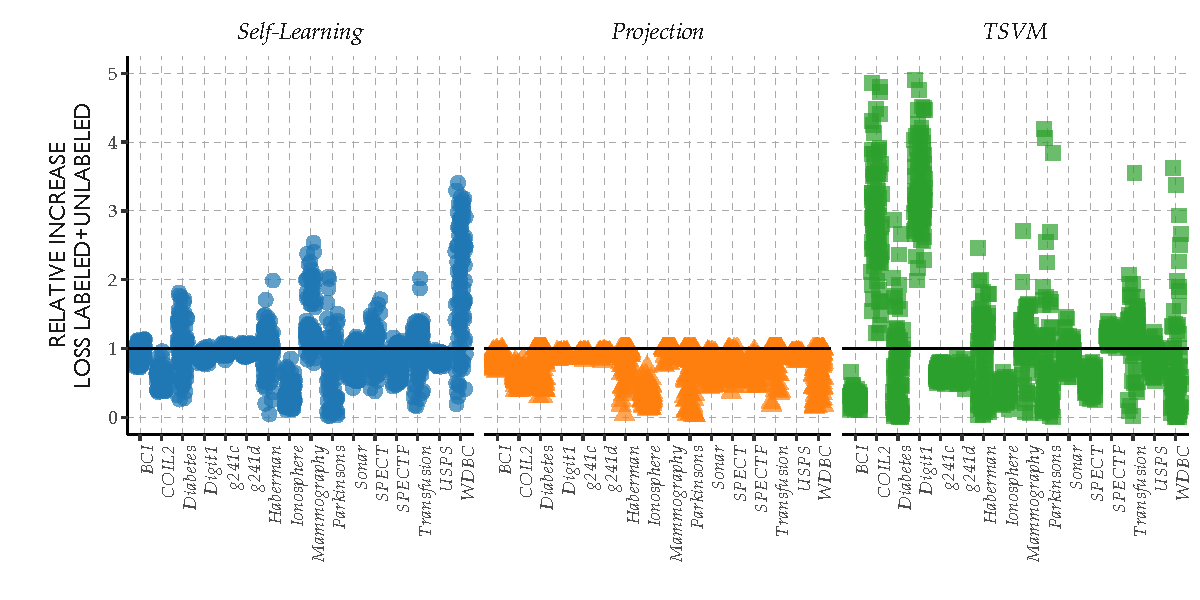
\includegraphics[width=\maxwidth]{figure/lossdifference-1} \caption{Ratio of the loss in terms of surrogate loss of supervised and semi-supervised solutions measured on the labeled and unlabeled instances. Values smaller than $1$ indicate that the semi-supervised method gives a lower average surrogate loss than its supervised counterpart. For both the projected estimator and self-learning this supervised counterpart is the supervised least squares classifier and loss is in terms of quadratic loss. For the $L_2$-Transductive SVM, quadratic hinge loss is used and compared to the quadratic hinge loss of a supervised $L_2$-SVM. Unlike the other semi-supervised procedures, the projection method, evaluated on labeled and unlabeled data, never has higher loss than the supervised procedure, as was proven in Theorem~\ref{th:robustness}.}\label{fig:lossdifference}
\end{figure}


\end{knitrout}

To illustrate Theorem \ref{th:robustness} experimentally, as well as study the performance of the proposed procedure on a test set, we set up the following experiment. For each of the $16$ datasets, we randomly select $2 d$ labeled objects. We then randomly sample, with replacement, $1000$ objects as the unlabeled objects from the dataset. In addition, a test set of $1000$ objects is also sampled with replacement. This procedure is repeated $100$ times and the ratio between the average quadratic losses for the supervised and the semi-supervised procedure $\tfrac{L(\vec{w}_\text{semi},\Xe,\vec{y}_\text{e}^{\ast})}{L(\vec{w}_\text{sup},\Xe,\vec{y}_\text{e}^{\ast})}$ is calculated. As stated by Theorem \ref{th:robustness}, this quantity should be smaller than $1$ for the Projection procedure. We do the same for self-learning applied to the least squares classifier and to an $L_2$-Transductive SVM, which we compare to the supervised $L_2$-SVM. The results are shown in Figure \ref{fig:lossdifference}. 

On the labeled and unlabeled data the loss of the projection method is lower than that of the supervised classifier in all of the resamplings taken from the original dataset. Compare this to the behaviour of the self-learner. While on average, the performance is quite similar on these datasets, on a particular sample from a dataset, self-learning may lead to a higher quadratic loss than the supervised solution. It is favourable to have no deterioration in every resampling because in practice one does not deal with resamplings from an empirical distribution, but rather with a single dataset. A semi-supervised procedure should ideally work on this particular dataset, rather than in expectation over all datasets that one might have observed. We see similar behaviour as self-learning for the difference in squared hinge loss between the $L_2$-SVM and the $L_2$-TSVM. While better parameter choices may improve the number of resamplings with improvements, this experiment illustrates that while semi-supervised methods may improve performance on average, for a particular sample from a dataset there is no guarantee like Theorem \ref{th:robustness} for the projected estimator. When looking at the difference in loss on an unseen test set, we find a similar results (not shown).

\subsection{Learning Curves}
To illustrate the behaviour of the procedure with increasing amounts of unlabeled data and to explore the relationship between the quadratic surrogate loss and classification accuracy on an unseen test set we generate learning curves in the following manner. For each of three illustrative datasets (Ionosphere, SPECT and USPS), we randomly sample $2 d$ objects as labeled objects. The remaining objects are used as a test set. For increasing subsets of the unlabeled data ($2,4,8,\dots,512$), randomly sampled without replacement, we train the supervised and semi-supervised learners and evaluate their performance on the test objects, in terms of classification accuracy as well as in terms of quadratic loss. We consider both the projection procedure where the distance measure is based on the labeled and the unlabeled data (denoted as Projection) as well as the projected estimator that only uses the labeled data in the distance measure (denoted as ICLS). The resampling is repeated $1000$ times and averages and standard errors are reported in Figure \ref{fig:learningcurves-projection}.

The first dataset (Ionosphere) in Figure \ref{fig:learningcurves-projection} is an example where the error of the self-learning procedure starts to increase once we add larger amounts of unlabeled data. In terms of the loss, however, the performance continues to increase. This illustrates that a decrease in the surrogate loss does not necessarily translates into a lower classification error. The projected estimators do not suffer from decrease in performance for larger numbers of unlabeled data in this example. In terms of the loss, however, there seems to be little difference between the three methods.

The second dataset (SPECT) is an example where both the self-learning procedure and the conservative projected estimator are not able to get any improvement out of the data, while the less conservative projection (ICLS) does show some improvement in terms of classification error.

On the USPS dataset the self-learning assumptions do seem to hold and it is able to attain a larger performance improvement as the amount of unlabeled data grows. Both in terms of the error and in terms of the loss, the projected estimators show smaller, but significant improvements.


\begin{knitrout}
\definecolor{shadecolor}{rgb}{1, 1, 1}\color{fgcolor}\begin{figure}
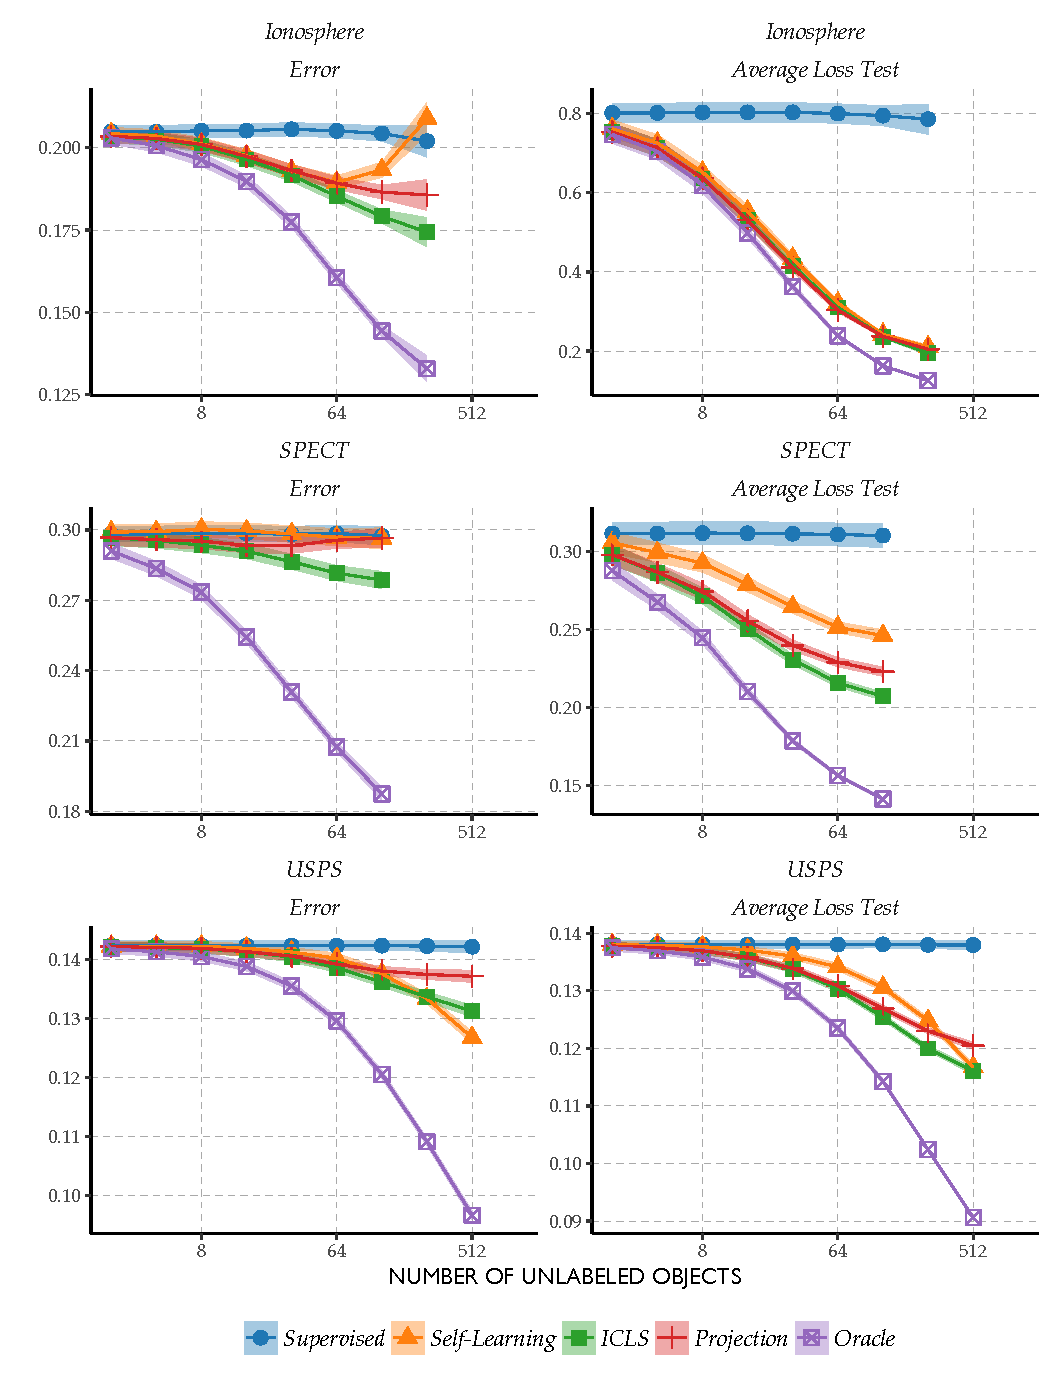
\includegraphics[width=\maxwidth]{figure/learningcurves-projection-1} \caption[Learning curves in terms of classification errors (top) and quadratic loss (bottom) on the test set for increasing numbers of unlabeled data on three illustrative datasets]{Learning curves in terms of classification errors (top) and quadratic loss (bottom) on the test set for increasing numbers of unlabeled data on three illustrative datasets. The lines indicate average errors respectively losses on the test set, averaged over 1000 repeats. The shaded bars indicate $\pm$ 2 standard errors around the mean.}\label{fig:learningcurves-projection}
\end{figure}


\end{knitrout}

\subsection{Cross-validation}
In a third experiment, we apply a cross-validation procedure to compare the performance increase in terms of the classification error of semi-supervised classifiers when compared to their supervised counterpart. The cross-validation experiments were set up as follows. For each dataset, the objects were split into 10-folds. Subsequently leaving out each fold, we combine the other 9 folds and randomly select $d+5$ labeled objects while the rest is used as unlabeled objects. We end up with a single prediction for each object, for which we evaluate the misclassification error. This procedure is repeated $20$ times and the averages are reported in Table~\ref{table:cvresults-projection}.

The results indicate that in terms of classification errors, the projection procedure never significantly reduces performance over the supervised solution. This is in contrast to the self-learner, which does significantly increase classification error on $2$ of the datasets. The price the projected estimator pays for this robustness, is smaller improvements over the supervised classifier than the less conservative self-learner. The Transductive SVM shows similar behaviour as the self-learner: it shows large improvements over the supervised alternative, but is also prone to degradation in performance on other datasets. The ICLS procedure is, as expected, less conservative than the projection method based on the labeled and unlabeled observations, which leads to larger improvements on all of the datasets.

\begin{table*}[t]
\center
\caption{20 repeat 10-fold cross-validation results for 16 datasets for the supervised least squares classifier, the projected least squares classifier (Projected), the projection based on only the labeled data (ICLS), the self-learned least squares classifier, the supervised $L_2$-SVM and the $L_2$-TSVM. \textbf{Bold} respectively \underline{Underlined} values indicate whether the performance of a semi-supervised solution is significantly better or worse than the supervised alternative as evaluated by a one-sided Wilcoxon signed rank test with family wise error rate of 0.05. The Win/Draw/Loss indicates on how many datasets a semi-supervised learner performs significantly better, equal or worse than the supervised alternative.} \label{table:crossvalidation-projection}
\label{table:cvresults-projection}
\scriptsize
\begin{tabular}{lllll|ll}
  \toprule
% latex table generated in R 3.4.1 by xtable 1.8-2 package
% Wed Nov  8 16:48:04 2017
Dataset & Supervised & Self-Learning & ICLS & Projection & SVM & TSVM \\ 
  \midrule
BCI & 0.40 $\pm$ 0.03 & \textbf{0.35 $\pm$ 0.02} & \textbf{0.28 $\pm$ 0.02} & \textbf{0.36 $\pm$ 0.03} & 0.30 $\pm$ 0.02 & 0.31 $\pm$ 0.02 \\ 
  COIL2 & 0.39 $\pm$ 0.01 & \textbf{0.26 $\pm$ 0.01} & \textbf{0.19 $\pm$ 0.01} & \textbf{0.34 $\pm$ 0.01} & 0.14 $\pm$ 0.01 & \underline{0.15 $\pm$ 0.01} \\ 
  Diabetes & 0.31 $\pm$ 0.02 & \underline{0.34 $\pm$ 0.01} & \textbf{0.30 $\pm$ 0.02} & \textbf{0.31 $\pm$ 0.02} & 0.36 $\pm$ 0.02 & \underline{0.38 $\pm$ 0.02} \\ 
  Digit1 & 0.42 $\pm$ 0.02 & \textbf{0.35 $\pm$ 0.02} & \textbf{0.20 $\pm$ 0.01} & \textbf{0.38 $\pm$ 0.01} & 0.06 $\pm$ 0.00 & 0.06 $\pm$ 0.01 \\ 
  g241c & 0.46 $\pm$ 0.01 & \textbf{0.39 $\pm$ 0.01} & \textbf{0.28 $\pm$ 0.01} & \textbf{0.42 $\pm$ 0.02} & 0.22 $\pm$ 0.01 & \textbf{0.21 $\pm$ 0.01} \\ 
  g241d & 0.44 $\pm$ 0.02 & \textbf{0.38 $\pm$ 0.01} & \textbf{0.29 $\pm$ 0.01} & \textbf{0.41 $\pm$ 0.02} & 0.23 $\pm$ 0.01 & \textbf{0.22 $\pm$ 0.01} \\ 
  Haberman & 0.29 $\pm$ 0.02 & 0.28 $\pm$ 0.02 & 0.29 $\pm$ 0.02 & 0.29 $\pm$ 0.02 & 0.29 $\pm$ 0.02 & 0.31 $\pm$ 0.03 \\ 
  Ionosphere & 0.28 $\pm$ 0.03 & \textbf{0.24 $\pm$ 0.01} & \textbf{0.19 $\pm$ 0.02} & \textbf{0.22 $\pm$ 0.03} & 0.20 $\pm$ 0.02 & 0.19 $\pm$ 0.02 \\ 
  Mammography & 0.30 $\pm$ 0.03 & 0.30 $\pm$ 0.02 & \textbf{0.29 $\pm$ 0.03} & 0.30 $\pm$ 0.03 & 0.30 $\pm$ 0.03 & 0.28 $\pm$ 0.02 \\ 
  Parkinsons & 0.25 $\pm$ 0.02 & 0.23 $\pm$ 0.03 & 0.24 $\pm$ 0.03 & 0.25 $\pm$ 0.03 & 0.22 $\pm$ 0.02 & 0.23 $\pm$ 0.02 \\ 
  Sonar & 0.44 $\pm$ 0.04 & \textbf{0.38 $\pm$ 0.04} & \textbf{0.33 $\pm$ 0.02} & \textbf{0.39 $\pm$ 0.02} & 0.26 $\pm$ 0.02 & \underline{0.33 $\pm$ 0.03} \\ 
  SPECT & 0.39 $\pm$ 0.04 & 0.38 $\pm$ 0.02 & \textbf{0.33 $\pm$ 0.03} & 0.39 $\pm$ 0.03 & 0.25 $\pm$ 0.03 & \textbf{0.20 $\pm$ 0.02} \\ 
  SPECTF & 0.44 $\pm$ 0.03 & \textbf{0.40 $\pm$ 0.04} & \textbf{0.36 $\pm$ 0.03} & \textbf{0.42 $\pm$ 0.03} & 0.25 $\pm$ 0.02 & \textbf{0.21 $\pm$ 0.01} \\ 
  Transfusion & 0.26 $\pm$ 0.02 & 0.28 $\pm$ 0.03 & 0.26 $\pm$ 0.02 & 0.26 $\pm$ 0.02 & 0.27 $\pm$ 0.01 & 0.28 $\pm$ 0.02 \\ 
  USPS & 0.42 $\pm$ 0.02 & \textbf{0.34 $\pm$ 0.02} & \textbf{0.20 $\pm$ 0.01} & \textbf{0.38 $\pm$ 0.02} & 0.11 $\pm$ 0.01 & \textbf{0.10 $\pm$ 0.00} \\ 
  WDBC & 0.09 $\pm$ 0.01 & \underline{0.13 $\pm$ 0.03} & \textbf{0.08 $\pm$ 0.01} & 0.09 $\pm$ 0.01 & 0.10 $\pm$ 0.01 & 0.11 $\pm$ 0.02 \\ 
   \midrule
Total &  & 9 / 5 / 2 & 13 / 3 / 0 & 10 / 6 / 0 &  & 5 / 8 / 3 \\ 
   \bottomrule

\end{tabular}
\end{table*}

% \begin{table*}[t]
% \center
% \caption{10-fold 20 repeat Cross-validation results for 16 datasets for the supervised least squares classifier, the projected least squares classifier (Projected), the projection based on only the labeled data (ICLS) and the self-learned least squares classifier. \textbf{Bold} respectively \underline{Underlined} values indicate whether the performance of a semi-supervised solution is significantly better or worse than the supervised alternative as evaluated by a one-sided Wilcoxon signed rank test with family wise error rate of $0.05$. The Win/Draw/Loss indicates on how many datasets a semi-supervised learner performs significantly better, equal or worse than the supervised alternative.}
% \smallskip
% \smallskip
% \smallskip
% % latex table generated in R 3.2.3 by xtable 1.8-0 package
% % Fri Feb  5 16:40:58 2016
% \begin{tabular}{|l|llll|ll|}
%    \hline
% Dataset & Supervised & Self-Learning & ICLS & Projection & SVM & TSVM \\ 
%   \hline
% BCI & 0.40 $\pm$ 0.03 & \textbf{0.35 $\pm$ 0.02} & \textbf{0.28 $\pm$ 0.02} & \textbf{0.36 $\pm$ 0.03} & 0.30 $\pm$ 0.02 & 0.31 $\pm$ 0.02 \\ 
%   COIL2 & 0.39 $\pm$ 0.01 & \textbf{0.26 $\pm$ 0.01} & \textbf{0.19 $\pm$ 0.01} & \textbf{0.34 $\pm$ 0.01} & 0.14 $\pm$ 0.01 & \underline{0.15 $\pm$ 0.01} \\ 
%   Diabetes & 0.31 $\pm$ 0.02 & \underline{0.34 $\pm$ 0.01} & \textbf{0.30 $\pm$ 0.02} & \textbf{0.31 $\pm$ 0.02} & 0.36 $\pm$ 0.02 & \underline{0.38 $\pm$ 0.02} \\ 
%   Digit1 & 0.42 $\pm$ 0.02 & \textbf{0.35 $\pm$ 0.02} & \textbf{0.20 $\pm$ 0.01} & \textbf{0.38 $\pm$ 0.01} & 0.06 $\pm$ 0.00 & 0.06 $\pm$ 0.01 \\ 
%   g241c & 0.46 $\pm$ 0.01 & \textbf{0.39 $\pm$ 0.01} & \textbf{0.28 $\pm$ 0.01} & \textbf{0.42 $\pm$ 0.02} & 0.22 $\pm$ 0.01 & \textbf{0.21 $\pm$ 0.01} \\ 
%   g241d & 0.44 $\pm$ 0.02 & \textbf{0.38 $\pm$ 0.01} & \textbf{0.29 $\pm$ 0.01} & \textbf{0.41 $\pm$ 0.02} & 0.23 $\pm$ 0.01 & \textbf{0.22 $\pm$ 0.01} \\ 
%   Haberman & 0.29 $\pm$ 0.02 & 0.28 $\pm$ 0.02 & 0.29 $\pm$ 0.02 & 0.29 $\pm$ 0.02 & 0.29 $\pm$ 0.02 & 0.31 $\pm$ 0.03 \\ 
%   Ionosphere & 0.28 $\pm$ 0.03 & \textbf{0.24 $\pm$ 0.01} & \textbf{0.19 $\pm$ 0.02} & \textbf{0.22 $\pm$ 0.03} & 0.20 $\pm$ 0.02 & 0.19 $\pm$ 0.02 \\ 
%   Mammography & 0.30 $\pm$ 0.03 & 0.30 $\pm$ 0.02 & \textbf{0.29 $\pm$ 0.03} & 0.30 $\pm$ 0.03 & 0.30 $\pm$ 0.03 & 0.28 $\pm$ 0.02 \\ 
%   Parkinsons & 0.25 $\pm$ 0.02 & 0.23 $\pm$ 0.03 & 0.24 $\pm$ 0.03 & 0.25 $\pm$ 0.03 & 0.22 $\pm$ 0.02 & 0.23 $\pm$ 0.02 \\ 
%   Sonar & 0.44 $\pm$ 0.04 & \textbf{0.38 $\pm$ 0.04} & \textbf{0.33 $\pm$ 0.02} & \textbf{0.39 $\pm$ 0.02} & 0.26 $\pm$ 0.02 & \underline{0.33 $\pm$ 0.03} \\ 
%   SPECT & 0.39 $\pm$ 0.04 & 0.38 $\pm$ 0.02 & \textbf{0.33 $\pm$ 0.03} & 0.39 $\pm$ 0.03 & 0.25 $\pm$ 0.03 & \textbf{0.20 $\pm$ 0.02} \\ 
%   SPECTF & 0.44 $\pm$ 0.03 & \textbf{0.40 $\pm$ 0.04} & \textbf{0.36 $\pm$ 0.03} & \textbf{0.42 $\pm$ 0.03} & 0.25 $\pm$ 0.02 & \textbf{0.21 $\pm$ 0.01} \\ 
%   Transfusion & 0.26 $\pm$ 0.02 & 0.28 $\pm$ 0.03 & 0.26 $\pm$ 0.02 & 0.26 $\pm$ 0.02 & 0.27 $\pm$ 0.01 & 0.28 $\pm$ 0.02 \\ 
%   USPS & 0.42 $\pm$ 0.02 & \textbf{0.34 $\pm$ 0.02} & \textbf{0.20 $\pm$ 0.01} & \textbf{0.38 $\pm$ 0.02} & 0.11 $\pm$ 0.01 & \textbf{0.10 $\pm$ 0.00} \\ 
%   WDBC & 0.09 $\pm$ 0.01 & \underline{0.13 $\pm$ 0.03} & \textbf{0.08 $\pm$ 0.01} & 0.09 $\pm$ 0.01 & 0.10 $\pm$ 0.01 & 0.11 $\pm$ 0.02 \\ 
%    \hline
% Total &  & 9 / 5 / 2 & 13 / 3 / 0 & 10 / 6 / 0 &  & 5 / 8 / 3 \\ 
%    \hline
% \end{tabular}
% \end{table*}

\subsection{Computational Considerations}
Since the projection proposed in Equation \eqref{eq:projection} can be formulated as a quadratic programming problem with a positive definite matrix, the worst case complexity is $O(N_u^3)$. Comparing this to Transductive SVM solvers, for instance, the CCCP procedure for Transductive SVMs by \cite{Collobert2006} has a worst case complexity of $O((N_l+2N_u)^3)$. The SVMlin implementation of \citet{Sindhwani2006} we compare to here makes few claims about its theoretical complexity. As \citet{Collobert2006} and \citet{Sindhwani2006} note, however, the practical complexity is often much lower than the worst case complexity and should be evaluated empirically. Figure~\ref{fig:timecomplexity} shows the computational time relative to the supervised classifier as we increase the number of unlabeled samples for our implementation of the Projection estimator and for the $L_2$-TSVM implementation of \citet{Sindhwani2006}. The figure shows that the SVMlin implementation scales much better as the number of unlabeled examples is increased. SVMlin's solution does not, however, guarantee that the solution is a global optimum, as the projection approach does, or guarantee any safe improvements over supervised learning. Whereas the explicit goal of SVMlin is to scale TSVM to larger datasets, we have not attempted to more efficiently solve the quadratic programming problem posed by our approach and leave this as an open problem.

\begin{knitrout}
\definecolor{shadecolor}{rgb}{1, 1, 1}\color{fgcolor}\begin{figure}
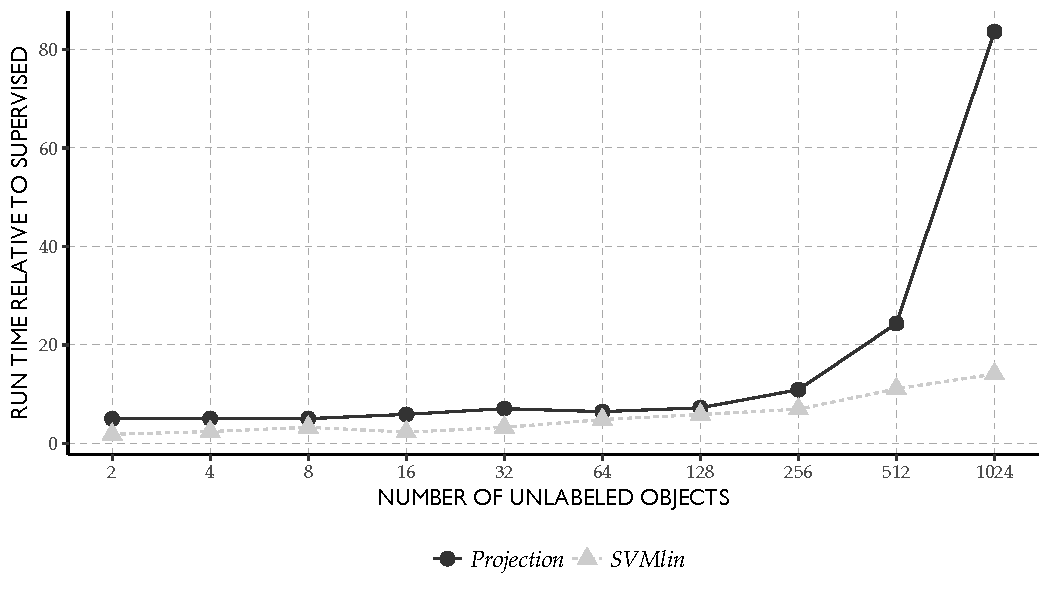
\includegraphics[width=\maxwidth]{figure/timecomplexity-1} \caption[Training time of semi-supervised methods relative to the training time of the supervised classifier for increasing amounts of unlabeled data on a simulated dataset with 2 Gaussian classes with $100$ features and $N_l=200$]{Training time of semi-supervised methods relative to the training time of the supervised classifier for increasing amounts of unlabeled data on a simulated dataset with 2 Gaussian classes with $100$ features and $N_l=200$.}\label{fig:timecomplexity}
\end{figure}


\end{knitrout}

\section{Discussion}
The main result of this work is summarized in Theorem \ref{th:robustness} and illustrated in Figure~\ref{fig:lossdifference}: the proposed semi-supervised classifier is guaranteed to improve over the supervised classifier in terms of the quadratic loss on all training data, labeled and unlabeled. The results from the experiments indicate that on average, both the projected estimator and other semi-supervised approaches often show improved performance, while on individual samples from the datasets, the projected estimator never reduces performance in terms of the surrogate loss. This is an important property since, in practical settings, one only has a single sample (i.e. dataset) from a classification problem, and it is important to know that performance will not be degraded when applying a semi-supervised version of a supervised procedure on that particular dataset. Even if we do not have enough labeled objects to accurately estimate this performance, Theorem \ref{th:robustness} guarantees we will not perform worse than the supervised alternative on the labeled and unlabeled data in terms of the surrogate loss. 

\subsection{Surrogate Loss}
Theorem~\ref{th:robustness} is limited to showing improvement in terms of quadratic loss. As the experiments also indicate, good properties in terms of this loss do not necessarily translate into good properties in terms of the error rate. In the empirical risk minimization framework, however, classifiers are constructed by minimizing surrogate losses. This particular semi-supervised learner is effective in terms of this objective. In this sense, it can be considered a proper semi-supervised version of the supervised quadratic loss minimizer.

One could question whether the quadratic loss is a good choice as surrogate loss \citep{Ben-David2012}. In practice, however, it can perform very well and is often on par and sometimes better than, for instance, an SVM employing hinge loss \citep{Rasmussen2005,Hastie2009,Poggio2003}. Moreover, the main result in this work basically demonstrates that strong improvement guarantees are at all possible for \emph{some} surrogate loss function. Whether and when an increase in performance in terms of this surrogate loss translates into improved classification accuracy is, like in the supervised setting, unclear. Much work is currently being done to understand the relationship between surrogate losses and ${0}-{1}$ loss \citep{Bartlett2006, Ben-David2012}. 

\subsection{Conservatism}
Arguably, a robust semi-supervised learning procedure could also be arrived at by very conservatively setting the parameters controlling the influence of unlabeled data in semi-supervised learner procedures such as the TSVM. There are two reasons why this is difficult to achieve in practice. The first reason is a computational one. Most semi-supervised procedures are computationally intensive. Doing a grid search over both a regularization parameter as well as the parameter controlling the influence of the unlabeled objects using cross-validation is time-consuming. Secondly, and perhaps more importantly, it may be very difficult to choose a good parameter using limited labeled data. \citet{Goldberg2009} study this problem in more detail. While their conclusion suggests otherwise, their results indicate that performance degradation occurs on a significant number of datasets. 

The projected estimator presented here tries to alleviate these problems in two ways. Firstly, unlike many semi-supervised procedures, it can be formulated as a quadratic programming problem in terms of the unknown labels which has a global optimum (which is unique in terms of $\vec{w}$) and there are no hyper-parameters involved. Secondly, at least in terms of its surrogate loss, there is a guarantee performance will not be worse than the alternative of discarding the unlabeled data. 
%Even approaches like those proposed by \citet{Li2011} require some assumptions about the data to hold to guarantee improvement.

As our results indicate, however, the proposed procedure is very conservative. The projection with $\mathbf{X}_\circ = \mathbf{X}$ (ICLS) is a classifier which is less conservative than the projection based on all data, and offers larger improvement in the experiments while still being robust to degradation of performance. For this procedure Theorem~\ref{th:robustness} does not hold.  Better understanding in what way we can still prove other robustness properties for this classifier is an open issue.

An alternative way to derive less conservative approaches could be by changing the constraint set $\Theta$. The purpose of this work has been to show that if we choose $\Theta$ conservatively, such that we can guarantee it contains the oracle solution $\vec{w}_\text{oracle}$, we can guarantee non-degradation, while still allowing for improved performance over the supervised solution in many cases. To construct a method with wider applicability, an interesting question is how to restrict $\Theta$ based on additional assumptions, while ensuring that $\vec{w}_\text{oracle} \in \Theta$ with high probability.

\subsection{Other Losses}
Another open question is for what other losses we can apply the projection procedure presented here. Apart from the issue of defining the metric in these cases, for some other loss functions the current definition of the constraint set might not constrain the parameter space at all. In the case of hinge loss or logistic loss, empirical results seem to indicate that the constraint set $\Theta$ always includes $\mathbf{w}_\mathrm{sup}$.  The lack of a closed-form solution, however, hampers a detailed theoretical analysis of these settings. Therefore, an exact characterization of the kinds of losses for which the procedure is amenable has to be left as an open problem.

\section{Conclusion}
We introduced and analyzed an approach to semi-supervised learning with quadratic surrogate loss that has the interesting theoretical property of never decreasing performance when measured on the full, labeled and unlabeled, training set in terms of this surrogate loss when compared to the supervised classifier. This is achieved by projecting the solution vector of the supervised least squares classifier onto a constraint set of solutions defined by the unlabeled data. As we have illustrated through simulation experiments, the safe improvements in terms of the surrogate loss on the labeled and unlabeled data also partially translate into safe improvements in terms of the classification errors on an unseen test set. Moreover, the procedure can be formulated as a standard quadratic programming problem, leading to a simple optimization procedure. An open problem is how to apply this procedure or a procedure with similar theoretical performance guarantees, to other loss functions.
\cleartoverso
\null
\thispagestyle{empty}
\newpagecolor{ThesisDark}\afterpage{\restorepagecolor}
\newpage
\renewcommand{\mypartpic}{cover/part2.pdf}
\AddToShipoutPicture{\PartPic}
\part{SURROGATE LOSSES}
\ClearShipoutPicture

\chapter[On Measuring and Quantifying Performance]{On Measuring and Quantifying Performance: Error Rates, Surrogate Loss,\\and an Example in SSL}
\chaptermark{Measuring and Quantifying Performance}
\label{chapter:quantifying}
\blfootnote{This chapter appeared as: Loog, M., Krijthe, J.H. \& Jensen, A.C., (2016). On Measuring and Quantifying Performance: Error Rates, Surrogate Loss, and an Example in SSL. In C. H. Chen, ed. Handbook of Pattern Recognition and Computer Vision. World Scientific.}



\begin{abstract}
In various approaches to learning, notably in domain adaptation, active learning, learning under covariate shift, semi-supervised learning, learning with concept drift, and the like, one often wants to compare a baseline classifier to one or more advanced (or at least different) strategies.  In this chapter, we basically argue that if such classifiers, in their respective training phases, optimize a so-called surrogate loss, then it may also be valuable to compare the behaviour of this loss on the test set, next to the regular classification error rate. It can provide us with an additional view on the classifiers' relative performances that error rates cannot capture.  As an example, limited but convincing empirical results demonstrate that we may be able to find semi-supervised learning strategies that can guarantee performance improvements with increasing numbers of unlabeled data in terms of log-likelihood.  In contrast, the latter may be impossible to guarantee for the classification error rate.
\end{abstract}


\section{Introduction}
The aim of semi-supervised learning is to improve supervised learners by exploiting potentially large amounts of, typically easy to obtain, unlabeled data \cite{Chapelle2006}.  Up to now, however, semi-supervised learners have reported mixed results when it comes to such improvements: it is not always the case that semi-supervision results in lower expected error rates.  On the contrary, severely deteriorated performances have been observed in empirical studies and theory shows that improvement guarantees can often only be provided under rather stringent conditions \cite{Castelli1995,Ben-David2008,Lafferty2007,Singh2008}.

Now, the principal suggestion put forward in this chapter is that, when dealing with semi-supervised learning, one may not only want to study the (expected) error rates these classifiers produce, but also to measure the classifiers' performances by means of the intrinsic loss they may be optimizing in the first place.  That is, for classification routines that optimize a so-called surrogate loss at training time---which is what many machine learning and Bayesian decision theoretic approaches do \cite{scholkopf2002learning,robert2001bayesian}, we propose to also investigate how this loss behaves on the test set as this can provide us with an alternative view on the classifier's behaviour that a mere error rate cannot capture.

In fact, though the main example is concerned with semi-supervision, we would like to argue that in other learning scenarios, similar considerations might be beneficial.  For instance in active learning \cite{settles2010active}, where rather than sampling randomly from ones input data to provide these instances with labels, one aims to do the sampling in a systematic way, trying to keep labeling cost as low as one can or, similarly, to learn from as few labeled examples as possible.  Also here it may (or, we believe, it should) be of interest to not only compare the error rates that different approaches (e.g. random sampling and uncertainty sampling \cite{lewis1994sequential}) achieve, but also how the surrogate losses compare for these techniques when we are using the same underlying classifiers.  Similar remarks can be made for other learning scenarios like domain adaptation, transfer learning, and learning under data shift or data drift \cite{margolis2011literature,torrey2009transfer,Quinonero-Candela2009,vzliobaite2010learning}.  In these last settings, one may typically want to compare, say, a classifier trained in a source domain with one that exploits additional knowledge on a target domain.


\subsection{Surrogate Loss vs. Error Rates}

The simple idea underlying the suggestion we make is that, unless we make particular assumptions, generally, we cannot expect to minimize the error rate if we are, in fact, optimizing a surrogate loss.  This surrogate loss is, to a large extent, chosen for computational reasons, but of course the hope is that, with increasing training set size, minimizing it will not only lead to improvements with respect to this surrogate loss but also with respect to the expected error rate.  This cannot be guaranteed in any strict way however.  To start with, the classifier's error rate itself can already act rather unpredictably.  A general result by Devroye demonstrates, for instance, that for any classifier there exists a classification problem such that the error rate converges at an arbitrarily slow rate to the Bayes error \cite{Devroye1982}.  If the classifier is not a universal approximator \cite{devroye1996probabilistic,steinwart05}, there is not even a guarantee that the Bayes error will ever be reached.  Worse even, in the case that we are dealing with such model misspecification, error rates might even go up with increasing numbers of training samples \cite{Loog2012}. This leads to the rather counterintuitive result that, in some cases, expected error rates might actually be improved by throwing arbitrary samples out of the training set.  The aforementioned considerations lead us, all in all, to speculate that any kind of generally valid (i.e., not depending on strong assumptions) expected performance guarantees, if at all possible in semi-supervised learning or any of the other aforementioned learning scenarios, can merely be obtained in terms of the surrogate loss of the classifier at hand.  Overall, these ideas are in line with those presented in \cite{Loog2014b}.


We could definitely imagine that, still, one takes the position that the mere loss that matters is the 0/1 loss and that it is this quantity that has to be minimized.  As far as we can see, however, taking this stance to the extreme, one cannot do anything else than try and directly minimize this 0/1 loss and face all the computational complications that go with it.  On a less philosophical level, one may claim that the 0/1 loss is, in the end, also not the loss that one is interested in.  One might actually have an application-relevant loss and in real applications (clinical, domestic, industrial, pedagogic, etc.) this is but seldom the 0/1 loss.  In fact, the true loss of interest related to a particular classification problem may ultimately be unknown.

For us there is, however, a more basic reason for studying the surrogate loss intrinsic to the classifier at hand. As a matter of a fact, a lower loss really means the model is better, in the sense that the estimated parameters get closer to those of the optimal classifier one would obtain if all data is labeled.  In the particular setting of semi-supervised learning, a decrease in expected loss, when adding unlabeled data, really indicates that the same effect---i.e., an improved model fit---is achieved as with adding more labeled data.  In our opinion, this seems the least we could ask for in a semi-supervised setting.  With this we still do not mean to claim that the surrogate loss is \emph{the} quantity to study, but it does give us a different perspective on the problem in various learning scenarios.  Finally, let us point out that the connection between the 0/1 loss and surrogate losses has in recent years attracted quite some attention.  Some papers investigating theoretical aspects for particular classes of loss functions, but also covering the design of such surrogate losses, are \cite{Ben-David2012,masnadi2008design,Nguyen2009,Reid2009,reid2010composite,scott2011surrogate}. These contributions follow earlier works such as \cite{Bartlett2006}, and \cite{Zhang2004}.




\subsection{Outline}

This chapter illustrates our point by means of two classifiers that optimize the log-likelihood of the model fit to the data. Clearly, this objective should be maximized, but taking minus the likelihood would turn it into a loss (which is sometimes referred to as the log loss).  The particular classifiers under consideration are the nearest means classifier (NMC) \cite{duda72a} and classical linear discriminant analysis (LDA) \cite{rao1948utilization}.    Next section starts off with a general reflection on these two classifiers after which two semi-supervised variations are introduced.  Section \ref{sect:exp} reports on the results of the experiments, comparing the semi-supervised learners and their supervised counterparts empirically.  The final section discusses our findings in the light of the point we would like to make and concludes this chapter.






\section{A Biased Introduction to Semi-Supervision}

\begin{knitrout}
\definecolor{shadecolor}{rgb}{1, 1, 1}\color{fgcolor}\begin{figure}
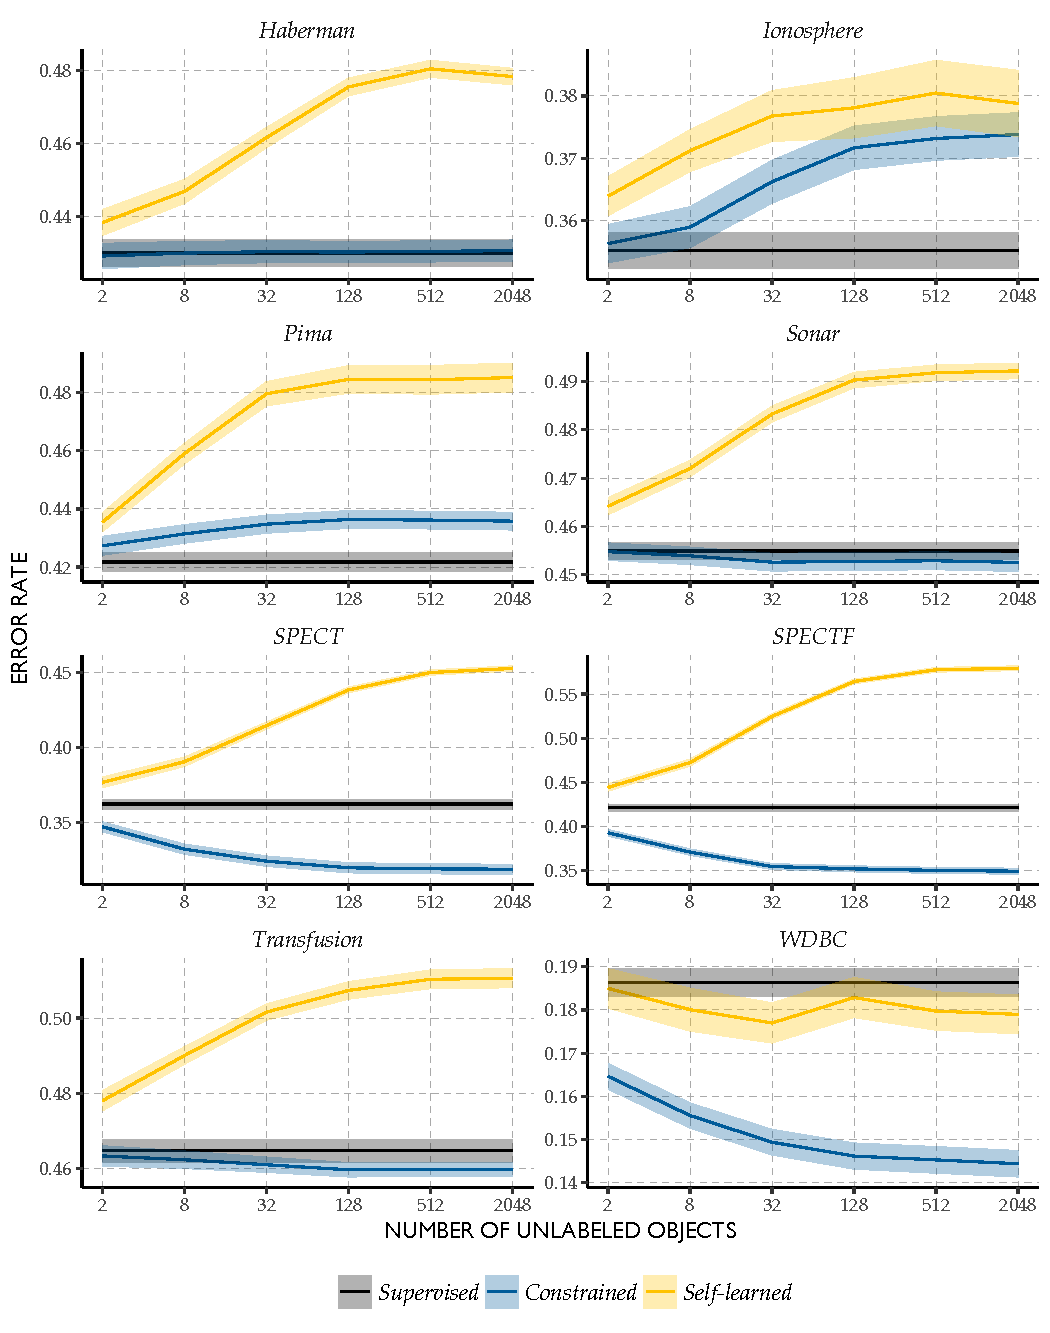
\includegraphics[width=\maxwidth]{figure/one-1} \caption[Mean error rates for the supervised (black), self-learned (yellow), and the constrained NMC (blue) on the eight real-world datasets for various unlabeled sample sizes and a total of four labeled training samples]{Mean error rates for the supervised (black), self-learned (yellow), and the constrained NMC (blue) on the eight real-world datasets for various unlabeled sample sizes and a total of four labeled training samples.}\label{fig:one}
\end{figure}


\end{knitrout}

Before we get to semi-supervised NMC and LDA, we feel the need to remark that their regular supervised versions are still capable of providing state-of-the-art performance. Especially for relatively high-dimensional, small sample problems NMC may be a particularly good choice.  Some rather recent examples demonstrating this can be found in bioinformatics and its applications \cite{wilkerson2012differential,villamil2012colon,budczies2012remodeling}, but also in neurology \cite{jolij2011act} and pathology \cite{gazinska2013comparison}. Further use of the NMC can be found in high-impact journals from the fields of oncology, neuroscience, general medicine, pharmacology, and the like.  A handful of the latest examples can be found in \cite{hyde2012mnemonic,haibe2012three,desmet2013identification,sjodahl2012molecular}.  Similar remarks can be made about LDA, though in comparison with the NMC, there should be relatively more data available to make it work at a competitive level.  Like for the NMC, many recent contributions from a large number of disciplines still employ this classical decision rule, e.g.\ \cite{ackermann2013detection,allen2013network,chung2013single,brunton2013rats,price2012cyanophora}.  All in all, like any other classifier, NMC and LDA have their validity and cannot be put aside as being outdated or not-state-of-the-art. The fact that classifiers having been around for 40 years or more, does not mean they are superseded.  In this respect, the reader might also want to consult relevant works such as \cite{Hand2006a} and \cite{efronXXX}.

\begin{knitrout}
\definecolor{shadecolor}{rgb}{1, 1, 1}\color{fgcolor}\begin{figure}
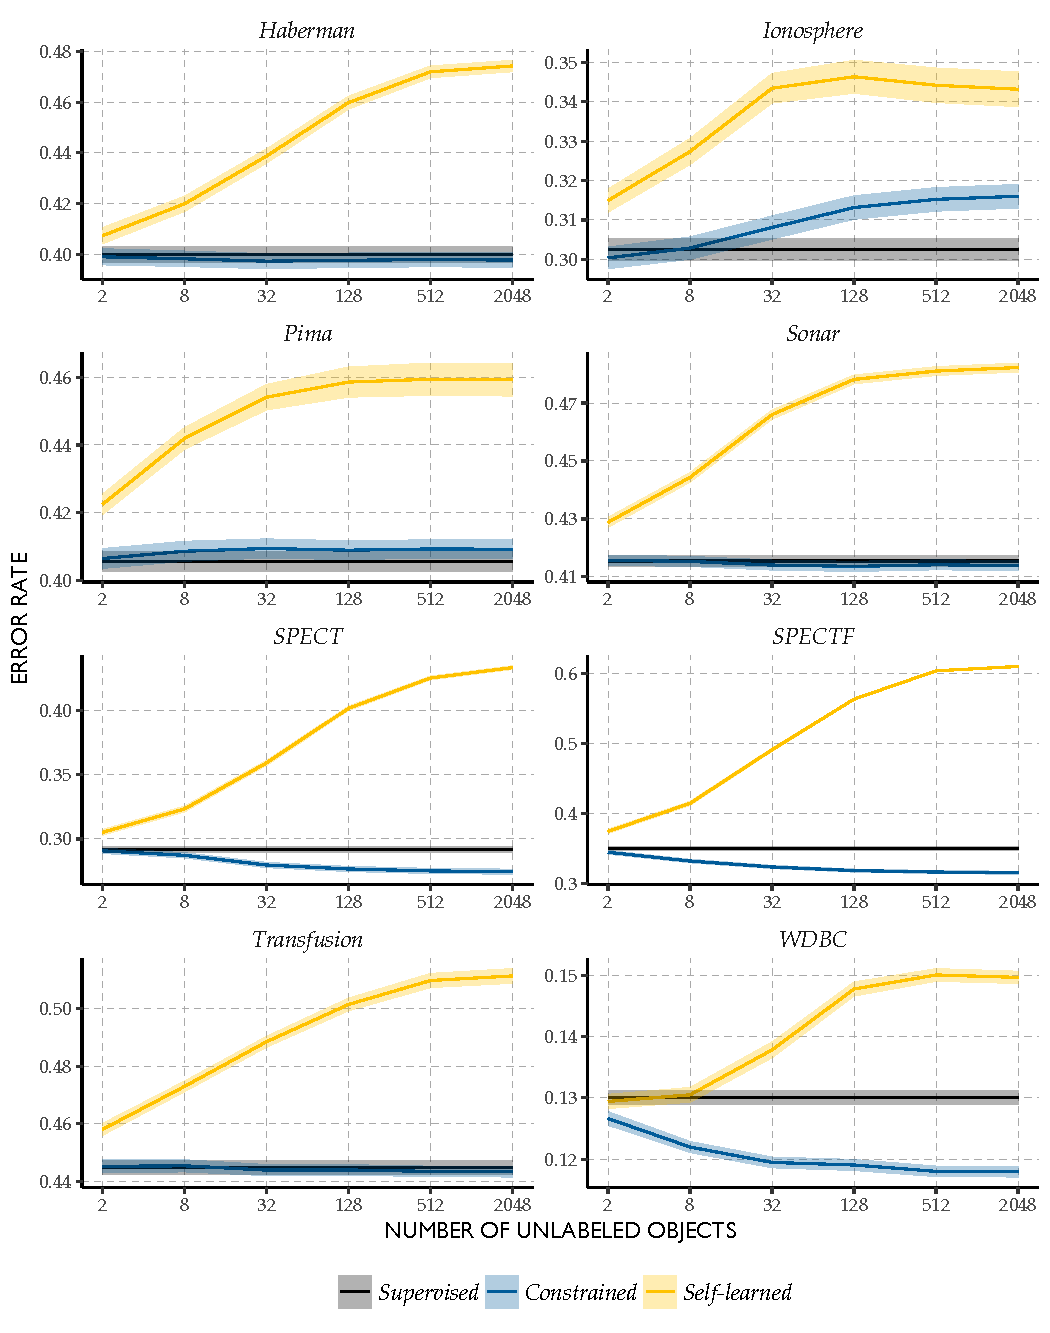
\includegraphics[width=\maxwidth]{figure/oneprime-1} \caption[Mean error rates for the supervised (black), self-learned (yellow), and the constrained NMC (blue) on the eight real-world datasets for various unlabeled sample sizes and a total of ten labeled training samples]{Mean error rates for the supervised (black), self-learned (yellow), and the constrained NMC (blue) on the eight real-world datasets for various unlabeled sample sizes and a total of ten labeled training samples.}\label{fig:oneprime}
\end{figure}


\end{knitrout}

\subsection{Supervised NMC and LDA}

The two semi-supervised versions of both the NMC and LDA are those based on classical expectation maximization or self-learning and those based on a so-called intrinsically constrained formulation.  These approaches are introduced in the subsections that follow.  The models underlying supervised NMC and LDA are based on normality assumptions for the class-conditional probability density functions.  More specifically:
\begin{itemize}

\item

LDA is the classical technique where the class-conditional covariance matrices are assumed the same across all classes, but where both the class means and the class priors can vary from class to class.  Estimating these variables under maximum likelihood results in the well-known solutions for the priors and the means, while the overall class covariance matrix becomes the prior weighted sum of the ML estimates of the individual class covariance matrices.

\item

For the NMC the parameter space is further restricted.  In addition to the covariance matrix being the same for all classes it is also constrained to be the a multiple of the identity matrix.  Moreover, the priors are fixed to be equal for all classes.  In \cite{Loog2014b} one can find the solution to this parameter estimation problem.  Here we note that this model is not necessarily unique: there are of course various ways in which one can formulate the NMC (as well as other classifiers) in terms of an optimization problem.  Ours is but one choice.

\end{itemize}


\subsection{EM and Self-Learning}



Self-learning or self-training is a rather generally applicable semi-supervised learning approach \cite{basu02a,McLachlan1975,vittaut02}.  In an initial step, the classifier of choice is trained on the available labeled data.  Using this trained classifier all unlabeled data is assigned a label.  Then, in a next step all of this now labeled data is added to the training set and the classifier is retrained with this enlarged set.  Given this newly trained classifier one can relabel the initially unlabeled data and retrain the classifier again with these updated labels.  This process is then iterated until convergence, i.e., when the labeling of the initially unlabeled data remains unchanged.  The foregoing only gives the basic recipe for self-learning.  Many variations and alternatives are possible.  One can, for instance, only take a fraction of the unlabeled data into account when retraining, once labeled one can decide to not relabel the data, etc.

Another well-known, and arguably more principled semi-supervised approach treats the absence of certain labels as a missing data problem. Most of the time this is formulated in terms of a maximum likelihood objective \cite{Dempster1977} and relies on the classical technique of expectation maximization (EM) to come to a solution \cite{nigam98a,ONeill1978}. Although self-learning and EM may at a first glance seem different ways of tackling the semi-supervised classification problem, \cite{basu02a} effectively shows that self-learners optimize the same objective as EM does (though they may typically end up in different local optima). Similar observations have been made in \cite{Abney2004,Haffari2007}.

A major problem with EM and self-learning strategies is the fact that they often suffer from severely deteriorated performance with increasing numbers of unlabeled samples. This behaviour, which has been extensively studied in various previous works \cite{cohen04a,Cozman2006,Loog2014a,yang2011effect}, is typically caused by model misspecification, i.e., the setting in which the statistical model does not fit the actual data distribution.  We note that this is at contrast with the supervised setting, where most classifiers are capable of handling mismatched data assumptions rather well and adding more labeled data typically improves performance.  NMC will most definitely suffer from model misspecification, because of the rather rigid, low-complexity nature of this classifier.  LDA is more flexible, but still only able to model linear decision boundaries.  Hence, also LDA will often be misspecified.


\subsection{Intrinsically Constrained NMC}
\begin{knitrout}
\definecolor{shadecolor}{rgb}{1, 1, 1}\color{fgcolor}\begin{figure}
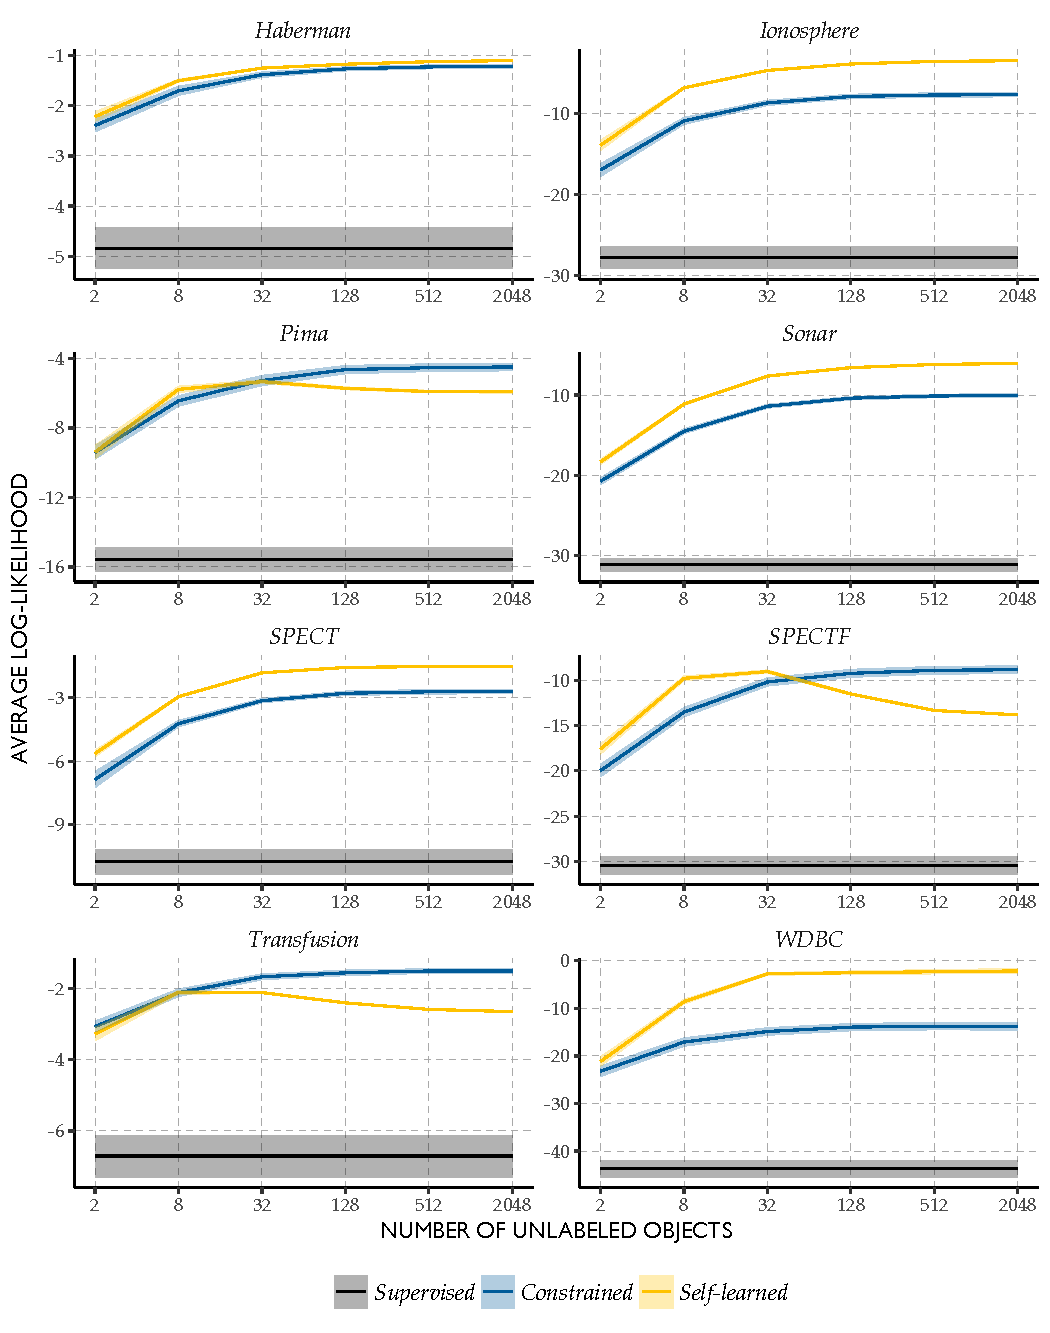
\includegraphics[width=\maxwidth]{figure/two-1} \caption{Mean log-likelihood for the supervised (black), self-learned (yellow), and the constrained NMC (blue) on the eight real-world datasets for various unlabeled sample sizes and a total of four labeled training samples.  Compare these to the respective error rates in Figure \ref{fig:one}.}\label{fig:two}
\end{figure}


\end{knitrout}
In \cite{Loog2010} and \cite{Loog2012a}, a novel way to learn in a semi-supervised manner was introduced.  On a conceptual level, the idea is to exploit constraints that are known to hold for the NMC and LDA and that define relationships between the class-specific parameters of those classifiers and certain statistics that are independent of the particular labeling.  These relationships are automatically fulfilled in the supervised setting but typically impose constraints in the semi-supervised setting.  Specifically, for NMC and LDA the following constraint holds (see \citet{fukunaga90}):
\begin{equation}\label{eq:altlaw}
N m = \sum_{k=1}^K N_k m_k \, ,
\end{equation}
where $K$ is the number of classes, $m$ is the overall sample mean of the data, and $m_k$ are the different sample means of the $K$ classes.  $N$ is the total number of training instances and $N_k$ is the number of observations for class $k$.  For LDA there is an additional constraint that holds (again see \citet{fukunaga90}):
\begin{equation}\label{eq:cov}
 B + W = T \, .
\end{equation}
It relates the standard estimates for the average class-conditional covariance matrix $W$, the between-class covariance matrix $B$, and the estimate of the total covariance matrix $T$.  $W$ is the covariance matrix that models the spread of every class in LDA.

In the supervised setting these constraints do not need to be assumed as they are automatically fulfilled.  Their benefit only becomes apparent with the arrival of unlabeled data. In the semi-supervised setting, the label-independent estimates $m$ and $T$ can be improved.  Using these more accurate estimates, however, results in a violation of the constraints. Fixing the constraints again by properly adjusting $m_i$, $W$, and $B$, these label-dependent estimates become more accurate and in expectation lead to improved classifiers.  For a more detailed account of how to enforce these constraints, we refer to \citet{Loog2014a} (see \citet{Krijthe2014} and \citet{Loog2012b} for related approaches).

The constrained estimation approach is less generally applicable, but it can avoid the severe deteriorations self-learning displays: when the model does not match the data, the model fit will obviously not be good, but the constrained semi-supervised fit will generally still be better, in terms of the error rate, than the supervised equivalent.  Still, also in this constrained setting, the results turn out not to be univocal either.  Error rates can increase with increasing number of unlabeled samples and we consider further insight into this issue paramount for a deeper understanding of the semi-supervised learning problem in general.




\section{Experimental Setup and Results}\label{sect:exp}

\begin{knitrout}
\definecolor{shadecolor}{rgb}{1, 1, 1}\color{fgcolor}\begin{figure}
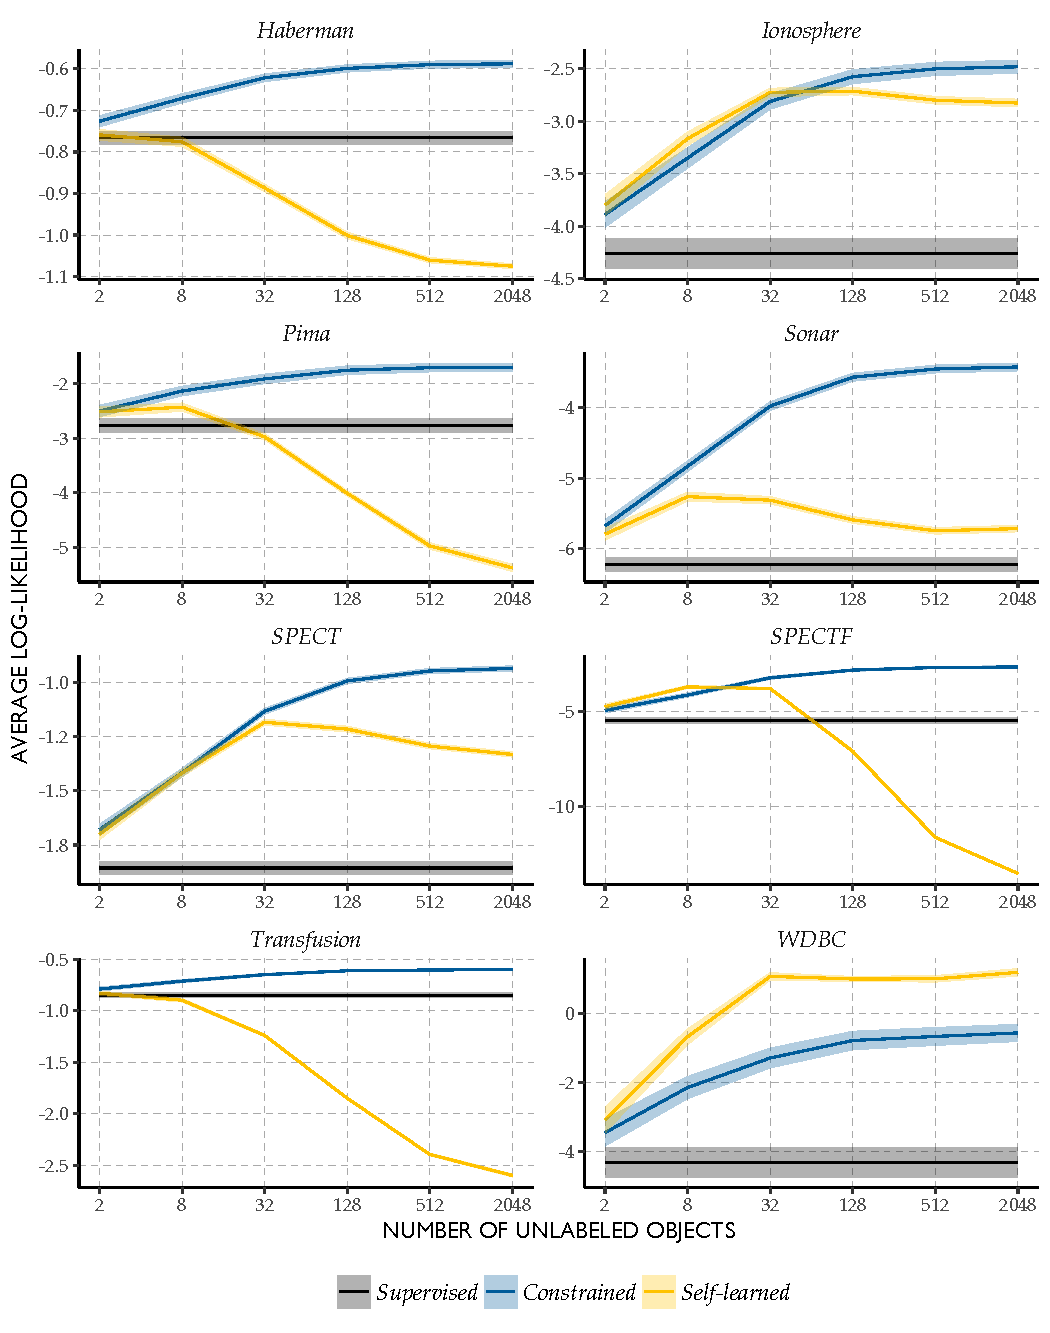
\includegraphics[width=\maxwidth]{figure/twoprime-1} \caption{Mean log-likelihood for the supervised (black), self-learned (yellow), and the constrained NMC (blue) on the eight real-world datasets for various unlabeled sample sizes and a total of ten labeled training samples.   Compare these to the respective error rates in Figure \ref{fig:oneprime}.}\label{fig:twoprime}
\end{figure}


\end{knitrout}

For the experiments, we used eight datasets from the UCI Machine Learning Repository \cite{Lichman2013}, all having two classes. The datasets used, together with some basic specifications, can be found in Table \ref{tab:real}.  We carried out the experiments in a way similar to those performed in \cite{Loog2014a}.




\begin{table}[ht]
\begin{center}
\caption{Basic properties of the eight two-class datasets from the UCI Machine Learning Repository \cite{Lichman2013}.}\label{tab:real}
\begin{tabular}{lccc}
\toprule
Data & Objects & Dimensions & Smallest Prior\\ 
\midrule
{ \scshape haberman } & 306 & 3 & 0.26 \\
{ \scshape ionosphere } & 351 & 33 & 0.36 \\
{ \scshape pima } & 768 & 8 & 0.35 \\
{ \scshape sonar } & 208 & 60 & 0.47 \\
{ \scshape spect } & 267 & 22 & 0.21 \\
{ \scshape spectf } & 267 & 44 & 0.21 \\
{ \scshape transfusion } & 748 & 3 & 0.24 \\
{ \scshape wdbc } & 569 & 30 & 0.37 \\
\bottomrule
\end{tabular}
\end{center}
\end{table}

Experiments with the three NMCs were done for two different total labeled training set sizes, four and ten, while the unlabeled training set sizes considered are $2^1=2$, $2^3$, \dots, $2^{9}$, and $2^{11} = 2048$.  For the supervised and semi-supervised LDAs, experiments were carried out with $100$ labeled samples and unlabeled training set sizes of $2^0=1$, $2^1$, \dots, $2^{12}$, and $2^{13} = 8196$. In the experiments, we study learning curves for increasing numbers of unlabeled data.  For every combination of the amount of unlabeled objects and labeled objects, 1000 repetitions of randomly drawn data were used to obtain accurate performance estimates.  In order to be able to do so based on the limited amount of samples provided by the datasets, instances were drawn with replacement.  This basically means that we assume that the empirical distribution of every dataset is its true distribution and this therefore allows us to measure the true error rates and the true log-likelihoods. It enabled us to properly study our learning curves on real-world data without having to deal with the extra variation due to cross validation and the like.


\begin{knitrout}
\definecolor{shadecolor}{rgb}{1, 1, 1}\color{fgcolor}\begin{figure}
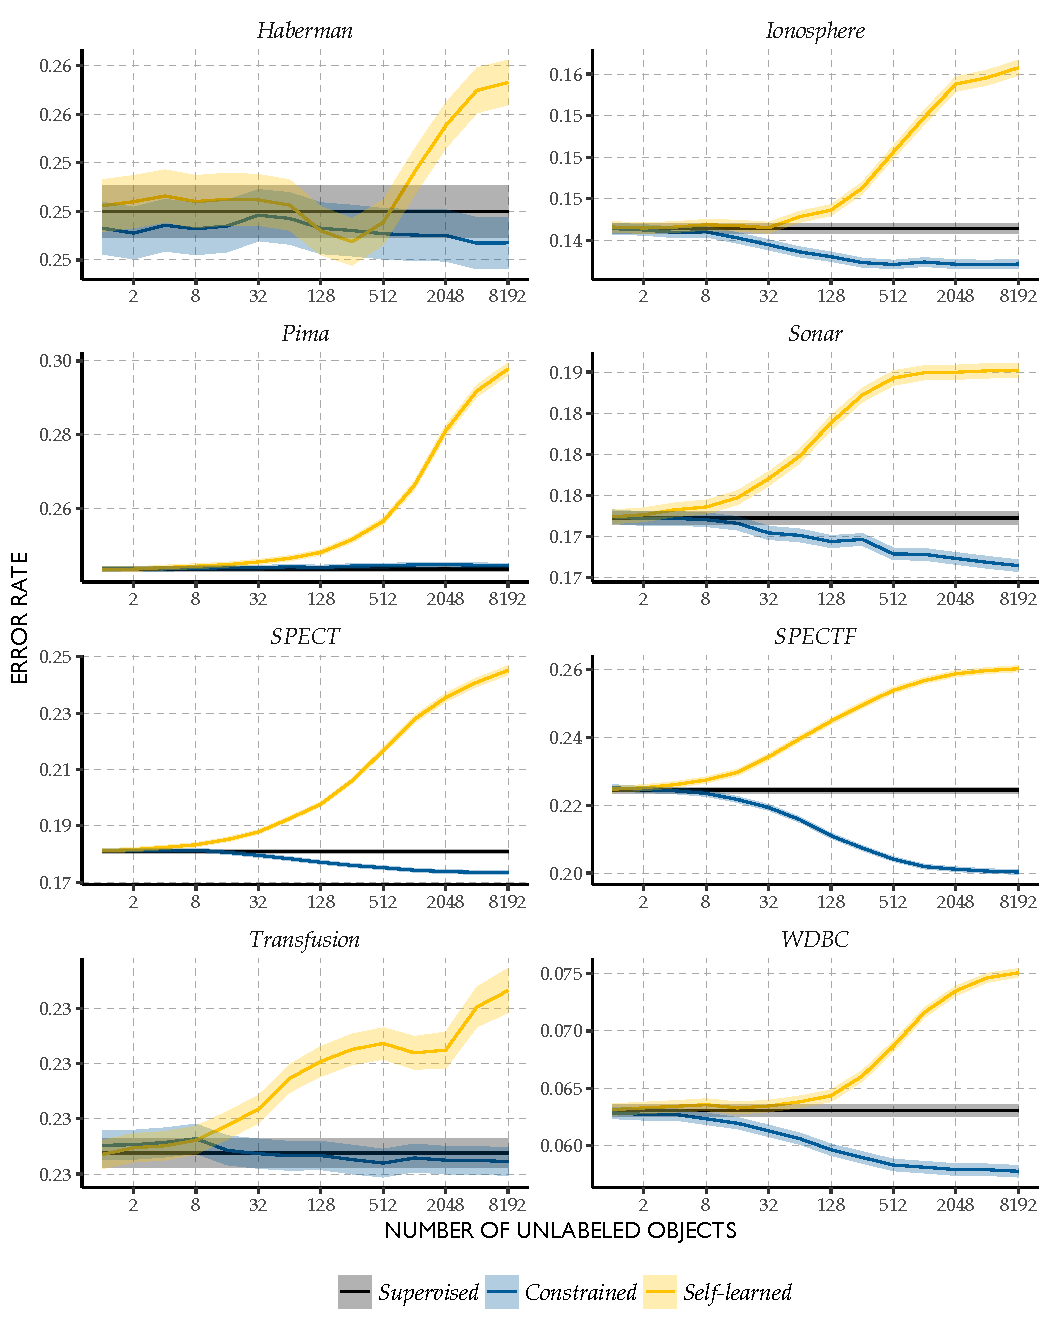
\includegraphics[width=\maxwidth]{figure/five-1} \caption[Mean error rates for supervised (black), self-learned (yellow), and constrained LDA (blue) on the eight real-world datasets for various unlabeled sample sizes and a total of 100 labeled training samples]{Mean error rates for supervised (black), self-learned (yellow), and constrained LDA (blue) on the eight real-world datasets for various unlabeled sample sizes and a total of 100 labeled training samples.}\label{fig:five}
\end{figure}


\end{knitrout}

\begin{knitrout}
\definecolor{shadecolor}{rgb}{1, 1, 1}\color{fgcolor}\begin{figure}
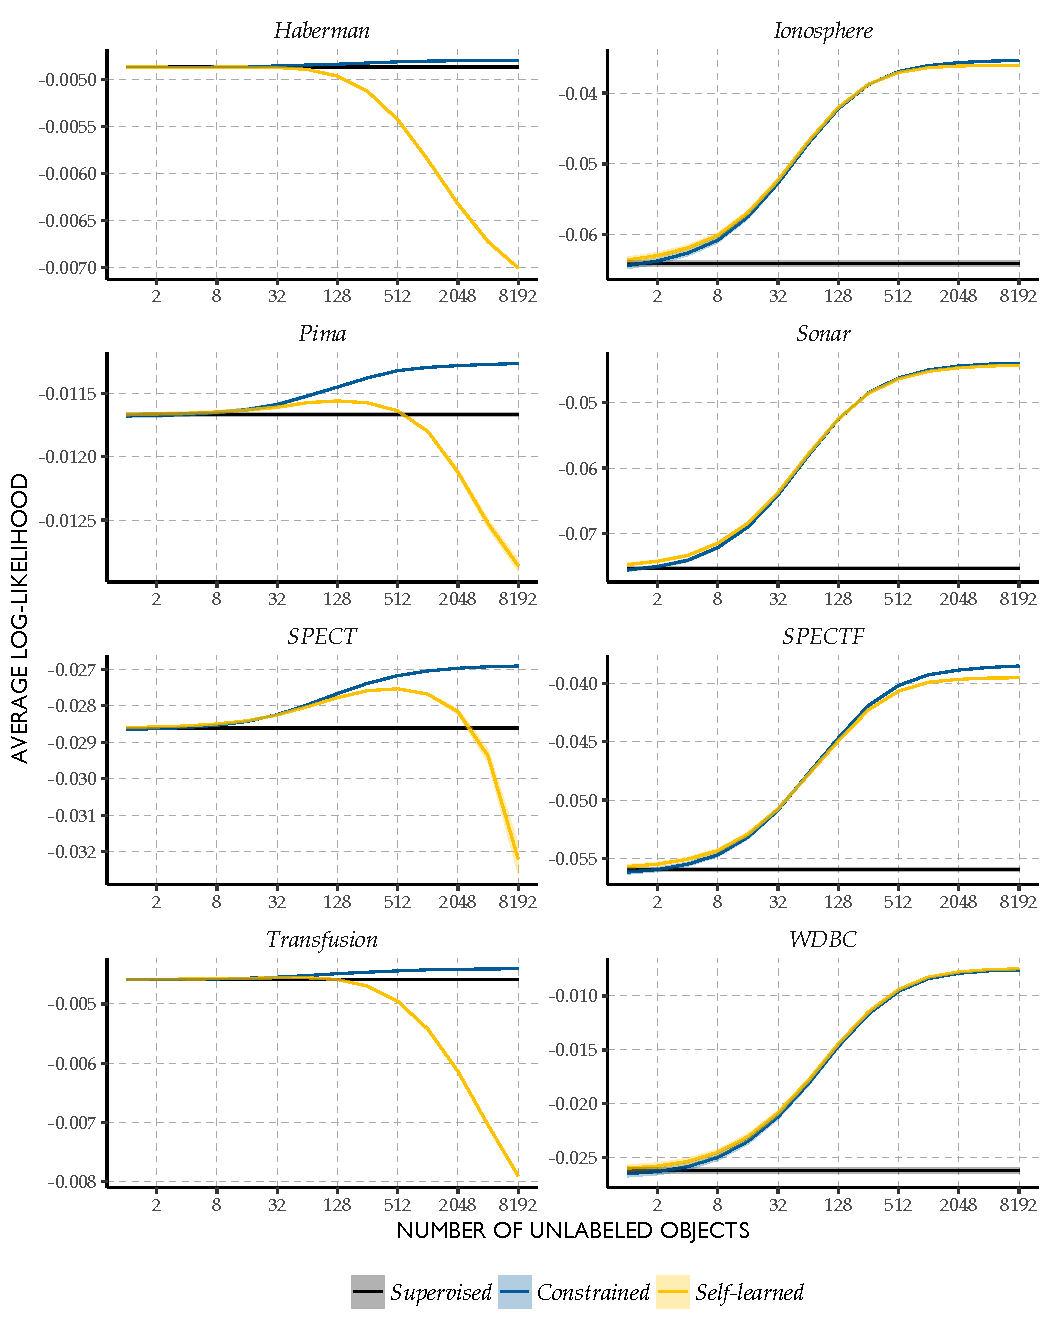
\includegraphics[width=\maxwidth]{figure/fiveprime-1} \caption{The curves for the log-likelihood of the three LDAs corresponding to the error curves in Figure \ref{fig:five}. }\label{fig:fiveprime}
\end{figure}


\end{knitrout}



Following the introductory section, we constructed learning curves both for the expected error rate and the expected log-likelihood (based on the 1000 repetitions).  Figure \ref{fig:one} shows the error rates for the NMCs on the various datasets when only four training samples are available.  Figure \ref{fig:oneprime} shows the error when ten samples are at hand.  The corresponding average log-likelihood curves can be found in Figures \ref{fig:two} and \ref{fig:twoprime}, respectively.  Figure \ref{fig:five} reports the error rates obtained with 100 training samples and using the supervised and semi-supervised LDAs.  Figure \ref{fig:fiveprime} reports on the corresponding log-likelihoods.   The supervised classification performance is displayed in black, self-learners are in yellow (NCS 0580-Y10R), and the constrained versions are in blue (NCS 4055-R95B). The lighter bands around the learning curves give an indication of the standard deviations of the averaged curves, providing an idea of the statistical significance of the differences between the curves.


\section{Discussion and Conclusion}\label{sect:fin}

To start with, it is important to note that when we look at the error rates, behaviours can indeed be quite disperse.  For both classifiers and both constrained and self-learned semi-supervised approaches, there are examples of error rates higher as well as lower than the averaged error rate the regular supervised learners achieve.  Sometimes rather erratic behaviour can be noted, like for self-learned NMC on {\scshape wdbc} in Figure \ref{fig:one} (yellow curve) and constrained LDA on {\scshape haberman} and {\scshape transfusion} in Figure \ref{fig:five} (blue curves).  On these last two, also the behaviour of self-learned LDA does not seem very regular.  Overall, the performance of the self-learners is very disappointing as only on {\scshape wdbc} with 4 labeled training samples, some overall but not very convincing improvements can be observed.  Regarding expected error rates, the constrained approach fares significantly better, showing clear performance improvement in at least 6 of the 16 NMC experiments and in 5 out of 8 of the LDA experiments.  Still, in at least 3 of the 16, classification errors become significantly worse for NMC and, in 5 out of 8 experiments, constrained LDA is not convincing.

Things drastically change indeed when we look at the log-likelihood curves.  For the constrained approaches, looking at Figure \ref{fig:two} and the lower half of Figure \ref{fig:fiveprime}, the story is very simple: where for the error rate deteriorations, improvements, and erraticism could be observed, the log-likelihood improves---i.e., increases---in every single case in a smooth, monotonic, and significant way.  Only for LDA on {\scshape haberman} and maybe {\scshape transfusion}, the constrained approach does not improve as convincingly as in all 22 other cases.

For self-learned NMC and LDA, the results are still mixed.  In many a case, we now do see improvements, but there are still some datasets on which the likelihood decreases.  Notably, for self-learned NMC with 4 labeled samples, the log-likelihood on the test data improves in all cases.  But we do not see the monotonic behaviour that the constrained approach displays.  Still, curves are less erratic than those for the error rates.  Nonetheless, it seems that even if we quantify performance in terms of log-likelihoods, we should be very critical towards self-learning and EM-based approaches. Behaviour definitely is much more regular in terms of its surrogate loss, but performances worse than the supervised approach provides still do occur.

Nevertheless, the results illustrate that it can be interesting to study not only the performance in terms of error rates but also in terms of the surrogate loss.  This is irrespective of the possibility that, ultimately, one might only be interested in the former.  It is encouraging to observe empirically that there seem to be semi-supervised learning schemes that can guarantee improvements in terms of the intrinsic surrogate loss.  This really is a nontrivial observation, as similar guarantees for error rates seem out of the question, unless strict conditions on the data are imposed; cf.\ \cite{Castelli1995,Ben-David2008,Lafferty2007,Singh2008}. Although our illustration is in terms of semi-supervised learning, it seems rather plausible that similar observations can be made for other learning settings in which two or more different estimation techniques for the same type of classifier, relying on the same surrogate loss, are compared.  All in all, it is worthwhile considering the behaviour of the surrogate in general, as it provides us with a view on a classifier's relative performance that a mere error rate cannot capture.

\chapter[The Pessimistic Limits of Margin-based Losses in Semi-supervised Learning]{The Pessimistic Limits of\\Margin-based Losses\\in Semi-supervised Learning}
\chaptermark{Margin-based Losses in SSL}
\label{chapter:marginbased}
\blfootnote{The work in this chapter has been submitted and was under review at the time of printing.}

\begin{abstract}
  % Semi-supervised learning has garnered much interest for its promise to improve learning algorithms by making use of abundant unlabeled data in learning scenarios where labeling is relatively expensive. While encouraging results have been obtained in some settings, in others, using unlabeled data has been shown to lead to a decrease in performance. This work is concerned with the limits of the applicability of pessimistic semi-supervised classification. It considers to what extent we can guarantee unlabeled data to improve a semi-supervised classifier compared to a supervised classifier evaluated on the labeled and unlabeled data in terms of its surrogate loss. In this sense, our analysis shows that for linear classifiers defined by convex margin-based surrogate losses that are monotonically decreasing, it is impossible to come up with \emph{any} semi-supervised approach that is able to guarantee a safe improvement in terms of this surrogate loss. For non-monotonically decreasing loss functions, safe improvements \emph{are} possible in terms of the loss considered. We describe the examples of logistic, hinge, quadratic, and absolute loss in more detail and discuss how our results relate to earlier claims that semi-supervised learning without additional assumptions is impossible.
  %
We show that for linear classifiers defined by convex margin-based surrogate losses that are monotonically decreasing,  it is impossible to construct \emph{any} semi-supervised approach that is able to guarantee an improvement over the supervised classifier measured by this surrogate loss. For convex margin-based loss functions that also increase, we demonstrate safe improvements \emph{are} possible.
\end{abstract}

\section{Introduction}

Semi-supervised learning has been reported to deliver encouraging results in various settings, e.g. for object detection in computer vision \citep{Rasmus2015}, protein function prediction from sequence data \citep{Weston2005} or prediction of cancer recurrence \citep{Shi2011} in the bio-medical domain and part-of-speech tagging in natural language processing \citep{Elworthy1994}.  In other settings, however, using unlabeled data has been shown to lead to a decrease in performance when compared to the supervised solution \citep{Elworthy1994, Cozman2006}. For semi-supervised classifiers to be used safely in practice, we may at least want some guarantee that they improve performance over their supervised alternatives. Some have attempted to provide such guarantees either empirically by restrictions on the parameters to be estimated \citep{Loog2010} or under particular assumptions on the data \citep{Li2015}. In general, however, it is unclear for what classifiers one can construct `safe' semi-supervised approaches that can be expected to not decrease performance, or whether this is at all possible.

\subsection{Safety and Pessimism}
This work is concerned with the limits of pessimistic semi-supervised classification. That is, we explore whether and, if so, how we can guarantee unlabeled data to improve, or at least not decrease the performance of a semi-supervised classifier in comparison to a supervised classifier. The `pessimism' refers to the property that we want this guarantee to hold for every single instantiation of a problem, even for the worst possible unknown labeling of the unlabeled data. The reason we choose such a strict criterion is that it is the only criterion that can guarantees (with probability one), that performance degradation will not occur, for the particular dataset one is faced with. Therefore, a semi-supervised approach can only be called truly safe if it guarantees non-degradation of performance in this pessimistic sense.

We compare the performance of the supervised and semi-supervised classifier measured on the labeled and unlabeled data. This is, strictly speaking, a transductive setting \cite{Joachims1999}, where one is interested in the performance on a specifically defined set of objects, and not a semi-supervised setting where one is interested in induction to unseen objects. As the number of unlabeled objects grows, however, and they start to better represent the distribution of interest in the inductive/semi-supervised setting, the limits and possibilities that we derive continue to hold.

\subsection{Surrogate Losses}
As our definition of performance, we consider the surrogate loss a classifier typically optimizes and compare this loss for the supervised and the semi-supervised learner on the combined labeled and unlabeled data. The surrogate loss corresponds to the loss one would minimize if we did have labels for the unlabeled objects. Considering the same criterion in the supervised and semi-supervised case aligns the goal of constructing a semi-supervised classifier with the one used when constructing a supervised classifier. By doing this, we avoid conflating improved performance based on a change in surrogate loss function with improvements gained by the availability of unlabeled data. For the same reason we also keep the regularization parameter fixed in the objective functions of the supervised and semi-supervised classifiers. 

In other words: we take the view that a semi-supervised version of, for instance, logistic regression is a classifier that still attempts to minimize logistic loss, but uses unlabeled data to improve its ability to do so. So it should be judged on how well it generalizes in terms of this intrinsic loss. If we were to compare performance in terms of some other loss, like the error rate, one runs the risk of attributing improvements to the use of unlabeled data that are, in fact, caused by other changes to the classifier. For instance, the semi-supervised classifier might implicitly use some other surrogate loss that turns out to be better aligned with the loss used for evaluation.

\subsection{Outline}
The main conclusion from our analysis (Theorems~\ref{theorem:hardlabels} and \ref{theorem:softlabels}) is that for classifiers defined by convex margin-based surrogate losses that are monotonically decreasing, it is impossible to come up with \emph{any} semi-supervised approach that is able to guarantee safe improvement. We also consider the case of non-monotonically decreasing losses and in particular explore the case of the quadratic loss.  We show under what conditions it \emph{is} possible in this case to come up with a semi-supervised classifier that provides safe improvements over the supervised classifier.

The rest of this work is structured as follows. We start by introducing margin-based loss functions in the empirical risk minimization framework and the extension to the semi-supervised setting.  In this, we only treat binary linear classifiers. Though not a real restriction, it does simplify our exposition and allows us to focus on the core ideas.  In Section~\ref{section:limits}, we formalize our strict notion of safe semi-supervised learning. We first show that for the class of monotonically decreasing loss functions it is impossible to derive any semi-supervised learning strategy that is not worse than the supervised classifier for all possible labelings of the unlabeled data. We then consider the case of soft assignment of unlabeled objects to classes. Here, too, it is impossible to provide a strict improvement guarantee for this class of loss functions.  We subsequently show for what losses it is possible to get strict improvements and discuss methods that use the idea of pessimism to construct semi-supervised classifiers. In Section~\ref{section:Examples} we apply the theory to a few well-known loss functions. In Section~\ref{section:Discussion} we discuss how these results relate to other results on the (im)possibility of (safe) semi-supervised learning and what the implications of these results are for approaches to safe semi-supervised learning.

\section{Preliminaries}
We consider binary linear classifiers in the empirical risk minimization framework. Let $\mathbf{X}$ be an $L \times d$ design matrix of $L$ labeled objects, where each row $\mathbf{x}^\top$ is a $d$-dimensional vector of feature values corresponding to each labeled object. Let $\mathbf{y} \in \{{-1},{+1}\}^L$ be the corresponding label vector. The vector $\mathbf{w} \in \mathbb{R}^d$ contains the weights defining a linear classifier through $\mathrm{sign}(\mathbf{x}^\top \mathbf{w})$. We consider convex margin-based surrogate loss functions, which are loss functions of the form $\phi(y \mathbf{x}^\top \mathbf{w})$. Many well-known classifiers can be described in this way, including logistic regression, least squares classification and support vector machines \citep{Bartlett2006} (see also Figure~\ref{figure:marginbasedlosses}).


\begin{knitrout}
\definecolor{shadecolor}{rgb}{1, 1, 1}\color{fgcolor}\begin{figure}
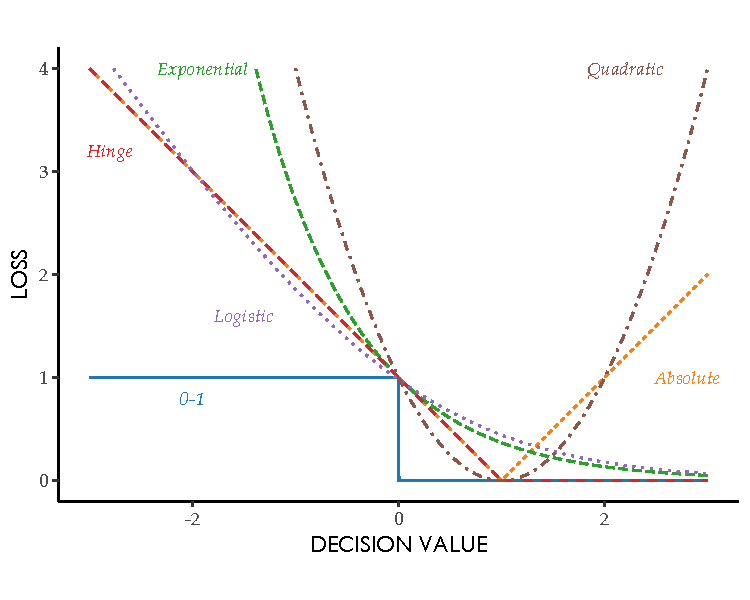
\includegraphics[width=\maxwidth]{figure/marginbasedlosses-1} \caption[Different Margin-based losses]{Different Margin-based losses}\label{figure:marginbasedlosses}
\end{figure}


\end{knitrout}


\subsection{Empirical Risk Minimization}

In the empirical risk minimization framework a classifier is obtained by minimizing a chosen surrogate loss $\phi$ over a set of training objects plus an optional regularization term $\Omega$, which we take to be a convex function of $\mathbf{w}$:
\begin{equation} \label{eq:supervisedrisk}
R_\phi(\mathbf{w},\mathbf{X},\mathbf{y}) = \sum_{i=1}^L \phi(y_i \mathbf{x}_i^\top \mathbf{w}) + \lambda \Omega(\mathbf{w})\, .
\end{equation}
By minimizing this with respect to $\mathbf{w}$ we get a supervised classifier:
$$\mathbf{w}_\mathrm{sup} = \argmin_\mathbf{w} R_\phi(\mathbf{w},\mathbf{X},\mathbf{y}) \, .$$

In the semi-supervised setting, we have an additional design matrix corresponding to unlabeled objects $\mathbf{X}_\mathrm{u}$, sized $U \times d$, with unknown labels $\mathbf{y}_\mathrm{u} \in \{{-1},{+1}\}^U$.
We therefore consider the corresponding semi-supervised risk function:
\begin{align} \label{eq:semisupervisedrisk}
 {R}^\mathrm{semi}_\phi(\mathbf{w},\mathbf{X},\mathbf{y},\mathbf{X}_\mathrm{u},\mathbf{q}) =  R_\phi(\mathbf{w},\mathbf{X},\mathbf{y}) + \sum_{i=1}^{U} q_i \phi(\mathbf{x}_i^\top \mathbf{w}) + (1-q_i) \phi(-\mathbf{x}_i^\top \mathbf{w}) \, ,
\end{align}
where $\mathbf{q} \in [0,1]^U$ are what we will refer to as \emph{responsibilities}, indicating the unknown and possibly `soft' membership of each object to a class. For instance, if the true labels were known these would correspond to `hard' responsibilities $\mathbf{q}^\mathrm{true} \in \{0,1\}^U$ and the semi-supervised risk formulation becomes equal to the supervised risk formulation in Equation \eqref{eq:supervisedrisk}, where the sum is now over the $L$ labeled objects and the $U$ objects for which we did not have a label.

\section{Limits of Safe Semi-supervision} \label{section:limits}

Even though we know the true labeling of the unlabeled objects in Equation (\ref{eq:semisupervisedrisk}) belongs to some $\mathbf{q} \in \{0,1\}^U$, we do not know which one. We say that a semi-supervised procedure $\mathbf{w}_\mathrm{semi}$ is \emph{safe} if it is guaranteed to attain a loss on the labeled and unlabeled objects equal to or lower than the supervised solution for all possible labelings of the data, since this is guaranteed to include the true labeling of the unlabeled objects.  In the remainder of this section we formalize this definition of safety, consider the cases of hard and soft labeling, and come to our negative results: for many loss functions safe semi-supervision is, in fact, not possible.

\subsection{Hard labeling}

Let $ {D}_\phi$ denote the difference in terms of the chosen loss $\phi$ on a set of objects between a new classifier $\mathbf{w}$ and the supervised classifier $\mathbf{w}_\mathrm{sup}$ for some set of responsibilities for the unlabeled data:
\begin{equation} \label{eq:difference}
{D}_\phi(\mathbf{w}_\mathrm{semi},\mathbf{w}_\mathrm{sup},\mathbf{X},\mathbf{y},\mathbf{X}_\mathrm{u},\mathbf{q}) =  {R}^\mathrm{semi}_\phi(\mathbf{w}_\mathrm{semi},\mathbf{X},\mathbf{y},\mathbf{X}_\mathrm{u},\mathbf{q}) \nonumber  - {R}^\mathrm{semi}_\phi(\mathbf{w}_\mathrm{sup},\mathbf{X},\mathbf{y},\mathbf{X}_\mathrm{u},\mathbf{q}) \, .
\end{equation}
The true unknown labels can in principle correspond to any $\mathbf{q} \in \{0,1\}^U$. For a semi-supervised classifier $\mathbf{w}_\mathrm{semi}$ to be \emph{safe} we therefore need that:
\begin{equation} \label{eq:hardcondition}
\max_{\mathbf{q} \in \{{0},{1}\}^U} {D}_\phi(\mathbf{w}_\mathrm{semi},\mathbf{w}_\mathrm{sup},\mathbf{X},\mathbf{y},\mathbf{X}_\mathrm{u},\mathbf{q}) \leq 0 \,.
\end{equation}
If the inequality is strict for at least one instantiation of $\mathbf{q}$, the semi-supervised solution is different from the supervised solution and potentially better.
Is it possible to construct some semi-supervised strategy  that has this guaranteed improvement over the supervised solution for margin-based surrogate losses? The following theorem gives a condition under which this strict improvement is never possible.

\begin{theorem} \label{theorem:hardlabels}
Let $\mathbf{w}_\mathrm{sup}$ be a minimizer of $ {R}_\phi(\mathbf{w},\mathbf{X},\mathbf{y})$ and assume it is unique. If $\phi$ is a monotonically decreasing convex margin-based loss function, meaning $\phi(a) \geq \phi(b)$ for $a\leq b$, then there is no safe semi-supervised procedure which guarantees Equation~\eqref{eq:hardcondition} while having at least one $\mathbf{q}^\ast$ for which $ {D}_\phi(\mathbf{w}_\mathrm{semi},\mathbf{w}_\mathrm{sup},\mathbf{X},\mathbf{y},\mathbf{X}_\mathrm{u},\mathbf{q}^\ast) < 0$\,.
\end{theorem}
\begin{proof}
We are going to prove this by contradiction. Let us start by assuming that ${D}_\phi(\mathbf{w}_\mathrm{semi},\mathbf{w}_\mathrm{sup},\mathbf{X},\mathbf{y},\mathbf{X}_\mathrm{u},\mathbf{q}^\ast) < 0$ and define $M$ to be $R_\phi(\mathbf{w}_\mathrm{semi},\mathbf{X},\mathbf{y})-R_\phi(\mathbf{w}_\mathrm{sup},\mathbf{X},\mathbf{y})$.  The latter is the difference in surrogate loss between the semi-supervised and supervised learner on the labeled data.   Based on our assumption we can now write
\begin{align} \label{eq:D_qast}
M + & \sum_{i=1}^{U}  q^\ast_i (\phi(\mathbf{x}_i^\top \mathbf{w}_\mathrm{semi})- \phi(\mathbf{x}_i^\top \mathbf{w}_\mathrm{sup})) & \\
 &+ (1-q^\ast_i) (\phi(-\mathbf{x}_i^\top \mathbf{w}_\mathrm{semi}) - \phi(-\mathbf{x}_i^\top \mathbf{w}_\mathrm{sup})) & < 0 \, . \nonumber
\end{align}

Let $A_i = \phi(\mathbf{x}_i^\top \mathbf{w}_\mathrm{semi})- \phi(\mathbf{x}_i^\top \mathbf{w}_\mathrm{sup})$ and $B_i = \phi(-\mathbf{x}_i^\top \mathbf{w}_\mathrm{semi})- \phi(-\mathbf{x}_i^\top \mathbf{w}_\mathrm{sup})$. Since $\phi$ is monotonically decreasing, either $A_i \geq 0$ and $B_i \leq 0$, or $A_i \leq 0$ and $B_i \geq 0$. Set $q^\mathrm{new}_i=1$ in the former case and $q^\mathrm{new}_i=0$ in the latter. Then, when using $\mathbf{q}^\mathrm{new}$ instead of $\mathbf{q}^\ast$ in Equation~\eqref{eq:D_qast}, the sum will be non-negative. Also, $M > 0$, because $\mathbf{w}_\mathrm{sup}$ is the unique minimizer of ${R}_\phi(\mathbf{w},\mathbf{X},\mathbf{y})$ and $\mathbf{w}_\mathrm{semi} \neq \mathbf{w}_\mathrm{sup}$. We therefore have that 
% \begin{align}
% &\sum_{i=1}^{U} q^\ast_i \phi(\mathbf{x}_i^\top \mathbf{w}_\mathrm{semi}) + (1-q^\ast_i) \phi(-\mathbf{x}_i^\top \mathbf{w}_\mathrm{semi}) \nonumber \\ & < \sum_{i=1}^{U} q^\ast_i \phi(\mathbf{x}_i^\top \mathbf{w}_\mathrm{sup}) + (1-q^\ast_i) \phi(-\mathbf{x}_i^\top \mathbf{w}_\mathrm{sup}) \, . \nonumber
% \end{align}
% Now consider the set of indices $i \in \mathcal{I}$ of all objects for which the loss of the semi-supervised solution is lower than the loss of the supervised solution, given the responsibility $\mathbf{q}^\ast$, i.e.,
% \begin{align}
% q^\ast_i & \phi(\mathbf{x}_i^\top \mathbf{w}_\mathrm{semi}) + (1-q_i^\ast) \phi(-\mathbf{x}_i^\top \mathbf{w}_\mathrm{semi}) \nonumber \\ & < q^\ast_i \phi(\mathbf{x}_i^\top \mathbf{w}_\mathrm{sup}) + (1-q_i^\ast) \phi(-\mathbf{x}_i^\top \mathbf{w}_\mathrm{sup}) \, . \nonumber
% \end{align}
% $\mathcal{I}$ is not empty, because by construction the total loss on the unlabeled objects for responsibility $\mathbf{q}^\ast$ is lower for $\mathbf{w}_\mathrm{semi}$ than for $\mathbf{w}_\mathrm{sup}$. For each $i \in \mathcal{I}$, either $q^\ast_i = 1$ or $q^\ast_i = 0$.
% If $q^\ast_i = 1$, $\phi(\mathbf{x}_i^\top \mathbf{w}_\mathrm{semi})<\phi(\mathbf{x}_i^\top \mathbf{w}_\mathrm{sup})$. Because $\phi$ is monotonically decreasing, it holds that $\mathbf{x}_i^\top \mathbf{w}_\mathrm{semi} > \mathbf{x}_i^\top \mathbf{w}_\mathrm{sup}$. We also have $-\mathbf{x}_i^\top \mathbf{w}_\mathrm{semi} < -\mathbf{x}_i^\top \mathbf{w}_\mathrm{sup}$ and because $\phi$ is monotonically decreasing $\phi(-\mathbf{x}_i^\top \mathbf{w}_\mathrm{semi}) \geq \phi(-\mathbf{x}_i^\top \mathbf{w}_\mathrm{sup})$.
% So changing label from $q^\ast_i = 1$ to $q^\mathrm{new}_i = 0$, the inequality is reversed. If $q^\ast_i = 0$, using the same argument, the inequality is also reversed if we choose $q^\mathrm{new}_i=1$ for these objects. This gives us
% \begin{align}
% q^\mathrm{new}_i & \phi(\mathbf{x}_i^\top \mathbf{w}_\mathrm{semi}) + (1-q_i^\mathrm{new}) \phi(-\mathbf{x}_i^\top \mathbf{w}_\mathrm{semi})\nonumber \\ & \geq q^\mathrm{new}_i \phi(\mathbf{x}_i^\top \mathbf{w}_\mathrm{sup}) + (1-q_i^\mathrm{new}) \phi(-\mathbf{x}_i^\top \mathbf{w}_\mathrm{sup}) \nonumber
% \end{align}
% for each  $i \in \mathcal{I}$. Since $i \in \mathcal{I}$ are the only objects for which the loss on the unlabeled objects decreased for the semi-supervised classifier compared and if we let $q_i^\mathrm{new}=q_i^\ast$ for $i \notin \mathcal{I}$ we have
$$ {D}_\phi(\mathbf{w}_\mathrm{semi},\mathbf{w}_\mathrm{sup},\mathbf{X},\mathbf{y},\mathbf{X}_\mathrm{u},\mathbf{q}^\mathrm{new}) > 0 \, ,$$
which contradicts Equation~\eqref{eq:hardcondition}.
% This shows that if there is some labeling $\mathbf{q}^\ast$ for which $\mathbf{w}_\mathrm{semi}$ leads to improved performance, it is always possible to construct a different labeling $\mathbf{q}^\mathrm{new}$ for which $\mathbf{w}_\mathrm{semi}$ leads to a worse performance than $\mathbf{w}_\mathrm{sup}$.
\end{proof}

\begin{remark}
Alternatively, we can drop the requirement that $\mathbf{w}_\mathrm{sup}$ is the unique minimizer of $ {R}_\phi(\mathbf{w},\mathbf{X},\mathbf{y})$ by requiring the loss functions to be strictly decreasing.
\end{remark}

% TODO: What happens when the constrast is applied to the unlabeled objects only?


\subsection{Beyond Hard Labelings}
In Equation \eqref{eq:hardcondition} we considered improvement over all hard labelings of the unlabeled data. Alternatively we could also consider improvements for the larger set of all soft assignments of labels to classes, defining safety to mean
\begin{equation} \label{eq:softcondition}
\max_{\mathbf{q} \in [0,1]^U} {D}_\phi(\mathbf{w}_\mathrm{semi},\mathbf{w}_\mathrm{sup},\mathbf{X},\mathbf{y},\mathbf{X}_\mathrm{u},\mathbf{q}) \leq 0 \,.
\end{equation}
If there is at least one $\mathbf{q} \in [0,1]^U$ for which the inequality is strict, the semi-supervised solution is potentially better than the supervised solution. There are several reasons why this is an interesting relaxation to consider. First of all it requires the semi-supervised solution to guarantee improvements for a larger class of responsibilities than just the hard labelings, meaning it becomes more difficult to construct a procedure with this property. If a procedure guarantees improvement in this sense, it implies it also works for all possible hard labelings. Secondly, it corresponds to a scenario different from the hard labeling where there is uncertainty in the labels of the unlabeled objects. And lastly, the convex constraint makes the problem more amenable to analysis and is, in fact, used by approaches such as MCPL \citep{Loog2016} and ICLS \citep{Krijthe2015}.

The set of classifiers given by all different responsibilities turns out to be a useful concept.
\begin{definition}\label{def:conset}
The constraint set $\mathcal{C}_\phi$ is the set of all possible classifiers that can be obtained by minimizing the semi-supervised loss for any vector of responsibilities $\mathbf{q}$ assigned to the unlabeled data, i.e.,
$$\mathcal{C}_\phi = \left\{ \argmin_\mathbf{w} {R}^\mathrm{semi}_\phi(\mathbf{w},\mathbf{X},\mathbf{y},\mathbf{X}_\mathrm{u},\mathbf{q}) \Big| \mathbf{q} \in [0,1]^U \right\} \, . $$
\end{definition}

The following lemma provides an intermediary step towards our second negative result.  It tells us that no strict improvement is possible if the supervised solution is already part of the constraint set.
\begin{lemma} \label{lemma:limitconstrainedspace}
If ${R}_\phi(\mathbf{w},\mathbf{X},\mathbf{y})$ is strictly convex and $\mathbf{w}_\mathrm{sup} \in \mathcal{C}_\phi$, then there is a soft assignment $\mathbf{q}^\ast$ such that for every choice of semi-supervised classifier $\mathbf{w}_\mathrm{semi} \neq \mathbf{w}_\mathrm{sup}$:  $${D}_\phi(\mathbf{w}_\mathrm{semi},\mathbf{w}_\mathrm{sup},\mathbf{X},\mathbf{y},\mathbf{X}_\mathrm{u},\mathbf{q}^\ast) > 0\,.$$
\end{lemma}
\begin{proof}
As $\mathbf{w}_\mathrm{sup} \in \mathcal{C}_\phi$ there is a soft labeling $\mathbf{q}^\ast$ such that $\mathbf{w}_\mathrm{sup}$ minimizes the semi-supervised risk ${R}^\mathrm{semi}_\phi(\mathbf{w},\mathbf{X},\mathbf{y},\mathbf{X}_\mathrm{u},\mathbf{q}^\ast)$.  This risk function is strictly convex because the supervised risk is strictly convex and therefore $\mathbf{w}_\mathrm{sup}$ is its unique minimizer.  This immediately implies that for every $\mathbf{w}_\mathrm{semi} \neq \mathbf{w}_\mathrm{sup}$, we have that $${R}^\mathrm{semi}_\phi(\mathbf{w}_\mathrm{semi},\mathbf{X},\mathbf{y},\mathbf{X}_\mathrm{u},\mathbf{q}^\ast) > {R}^\mathrm{semi}_\phi(\mathbf{w}_\mathrm{sup},\mathbf{X},\mathbf{y},\mathbf{X}_\mathrm{u},\mathbf{q}^\ast)\,.$$
\end{proof}
\begin{remark}
The requirement to have a strictly convex supervised risk function can be relaxed.  What we basically need in the proof is that $\mathbf{w}_\mathrm{sup}$ is the unique optimizer for ${R}^\mathrm{semi}_\phi(\mathbf{w},\mathbf{X},\mathbf{y},\mathbf{X}_\mathrm{u},\mathbf{q}^\ast)$.  Nevertheless, unlike, for instance, a hinge loss that is not regularized by something like a $2$-norm of the weight vector, many interesting objective functions are strictly convex.
\end{remark}

For monotonically decreasing margin-based losses, we now show that we can always explicitly construct a $\mathbf{q}^\ast$, such that the corresponding semi-supervised solution equals the original supervised one.  With this, a result similar to Theorem~\ref{theorem:hardlabels} for the soft-assignment guarantee directly follows, but first we formulate that explicit construction of the necessary soft labeling.
\begin{lemma}\label{lemma:responsibilities}
If $\phi$ is a monotonically decreasing margin-based loss function where for each unlabeled object $\mathbf{x}$, $\phi'(-\mathbf{x}^\top \mathbf{w}_\mathrm{sup})$ and $\phi'(\mathbf{x}^\top \mathbf{w}_\mathrm{sup})$ exist, we can recover $\mathbf{w}_\mathrm{sup}$ by minimizing the semi-supervised loss by assigning  responsibilities $\mathbf{q} \in [0,1]^U$ as follows:
\begin{equation}\label{eq:solutionq}
q = \frac{\phi'(-\mathbf{x}^\top \mathbf{w}_\mathrm{sup})}{\phi'(\mathbf{x}^\top \mathbf{w}_\mathrm{sup}) + \phi'(-\mathbf{x}^\top \mathbf{w}_\mathrm{sup})}\,.
\end{equation}
\end{lemma}

\begin{proof}
Consider the case where we have one unlabeled object $\mathbf{x}$ with responsibility $q$. The semi-supervised objective then becomes
\begin{align}
{R}^\mathrm{semi}_\phi (\mathbf{w})  = & {R}^\mathrm{sup}_\phi(\mathbf{w},\mathbf{X},\mathbf{y}) \nonumber \\
& + q \phi(\mathbf{x}^\top \mathbf{w}) + (1-q) \phi(-\mathbf{x}^\top \mathbf{w}) \, . \nonumber
\end{align}
We need to find a $q \in [0,1]$ that causes the gradient of this objective, evaluated in the supervised solution, to remain equal to zero:
\begin{equation}\label{eq:qequality}
\begin{split}
\nabla_{\mathbf{w}}  {R}_\phi^\mathrm{semi}({\mathbf{w}_\mathrm{sup}}) = &\,  \mathbf{0} + q \phi'(\mathbf{x}^\top \mathbf{w}_\mathrm{sup}) \mathbf{x} \\
& \,\,\,\,\, - (1-q) \phi'(-\mathbf{x}^\top \mathbf{w}_\mathrm{sup}) \mathbf{x}  \\
% & + 2 (\lambda-\mu) \mathbf{w}_\mathrm{sup} \\
= & \,  \mathbf{0}
\end{split}
\end{equation}
where $\phi'$ denotes the derivative of $\phi(a)$ with respect to $a$. As long as $\phi'(\mathbf{x}^\top \mathbf{w}_\mathrm{sup}) + \phi'(-\mathbf{x}^\top \mathbf{w}_\mathrm{sup}) \neq 0$, we can explicitly solve for $q$ to get
\begin{equation}
q = \frac{\phi'(-\mathbf{x}^\top \mathbf{w}_\mathrm{sup})}{\phi'(\mathbf{x}^\top \mathbf{w}_\mathrm{sup}) + \phi'(-\mathbf{x}^\top \mathbf{w}_\mathrm{sup})} \,.
\end{equation}
If $\phi$ is a monotonically decreasing loss, then
$$ \phi'(a) \leq 0 $$
and for each object $0 \leq q\leq 1$. Since this can be done for each object individually, we can do it for all objects to get a vector of responsibilities $\mathbf{q} \in [0,1]^U$.
\end{proof}

Now that we have shown by a constructive argument that for monotonically decreasing margin-based losses it always holds that  $\mathbf{w}_\mathrm{sup} \in \mathcal{C}_\phi$, the following result is straightforward.
\begin{theorem} \label{theorem:softlabels}
Let $\phi$ be a monotonically decreasing convex margin-based loss function and $\mathbf{w}_\mathrm{sup}$ be the unique minimizer of $ {R}_\phi(\mathbf{w},\mathbf{X},\mathbf{y})$. There is no semi-supervised classifier $\mathbf{w}_\mathrm{semi}$ for which Equation~\eqref{eq:softcondition} holds, while having at least one $\mathbf{q}^\ast$ for which $$ {D}_\phi(\mathbf{w}_\mathrm{semi},\mathbf{w}_\mathrm{sup},\mathbf{X},\mathbf{y},\mathbf{X}_\mathrm{u},\mathbf{q}^\ast) < 0\,.$$
\end{theorem}

\begin{proof}
This follows directly from Lemma~\ref{lemma:limitconstrainedspace} and Lemma~\ref{lemma:responsibilities}.
\end{proof}

This means that for monotonically decreasing loss functions it is impossible to construct a semi-supervised learner that is different from the supervised learner and, in terms of its surrogate loss on the full training data, is never outperformed by the supervised solution.  In other words, if the semi-supervised classifier is taken to be different from the supervised classier, there is always the risk that there is a true labeling of the unlabeled data for which the loss of the semi-supervised learner on the full data becomes larger than the loss of the supervised one.

Is it unexpected that semi-supervised learning cannot be done safely in this setting?  For whom it is not, it may then come as a surprise that there are margin-based losses for which it is actually possible to construct safe semi-supervised learners.

%
% \subsection{Different regularization terms}
% What happens if an additional regularization term $\mu \Omega(\mathbf{w})$ is added to the semi-supervised loss?
%
% Looking at Equation \eqref{eq:derivsemi} while considering multiple unlabeled objects, we have:
% \begin{align} \label{eq:derivsemi}
% \nabla_{\mathbf{w}} \mathcal{R}_\mathrm{semi}({\mathbf{w}_\mathrm{sup}}) = &  \mathbf{0} \\ \nonumber
% & + \sum_{i=1}^U q_i \phi'(\mathbf{x_i}^\top \mathbf{w}_\mathrm{sup}) \mathbf{x_i} - (1-q_i) \phi'(-\mathbf{x_i}^\top \mathbf{w}_\mathrm{sup}) \mathbf{x_i}^\top \mathbf{w}_\mathrm{sup}) \\ \nonumber
%  & + 2 (\mu) \mathbf{w} \\ \nonumber
% = &  \mathbf{0} \nonumber
% \end{align}
%
% When we have little data, this is an overdetermined system. As the number of unlabeled objects increases we can find a q, but it is not clear whether this q is within the bounds $[0,1]$.
%
% What happens when $\mu>\lambda$ and why does this make sense? (Stronger regularization, so we need to update anyway)
% What happens when $\mu<\lambda$ and why does this make sense? Numerical example. Consider the case where we have $100000$ objects and $1$ unlabeled object. This shows it might not make sense to omit the regularization term in the semi-supervised objective function.

\section{Possibilities for Safe SSL}
If we look beyond the previous losses, and consider non-monotonically decreasing ones, we may still be able to get a classifier that is guaranteed to be better than the supervised solution in terms of the surrogate loss, even in the pessimistic regime.
When can we expect safe semi-supervised learning to allow for improvements of its supervised counterpart?
And if improvements are possible, how then do we construct an actual classifier that does so in a safe way?

To construct a semi-supervised learner that at least is guaranteed to never be worse, we need to find $\mathbf{w}_\mathrm{semi}$, the $\mathbf{w}$ that minimizes $ {D}_\phi(\mathbf{w},\mathbf{w}_\mathrm{sup},\mathbf{X},\mathbf{y},\mathbf{X}_\mathrm{u},\mathbf{q})$ for all possible $\mathbf{q}$.  This corresponds, more precisely, to the following minimax problem:
\begin{equation} \label{eq:minmaxproblem}
\min_{\mathbf{w}} \max_{\mathbf{q} \in [0,1]^U} {D}_\phi(\mathbf{w},\mathbf{w}_\mathrm{sup},\mathbf{X},\mathbf{y},\mathbf{X}_\mathrm{u},\mathbf{q}) \, .
\end{equation}
This is a formulation similar to the one used by \citet{Loog2016}, where instead of margin-based losses, the loss functions are log-likelihoods of a generative model. It is clear that Equation~\eqref{eq:minmaxproblem} can never be larger than 0.  This simply indicates that we can always find a semi-supervised learner that is at least as good as the supervised one, by simply sticking to the supervised solution. To show that we can sometimes do better than that, consider the following.

If ${R}_\phi^\mathrm{semi}$ is convex in $\mathbf{w}$, then since the objective is linear in $\mathbf{q}$ and $[0,1]^U$ is a compact space we can invoke \citep[Corrolary 3.3]{Sion1958}, which states that the value of the minimax problem is equal to the value of the maximin problem:
\begin{equation} \label{eq:minmaxproblem2}
 \max_{\mathbf{q} \in [0,1]^U} \min_{\mathbf{w}} {D}_\phi(\mathbf{w},\mathbf{w}_\mathrm{sup},\mathbf{X},\mathbf{y},\mathbf{X}_\mathrm{u},\mathbf{q}) \, .
\end{equation}
Assume the function ${D}_\phi$ is strictly convex in $\mathbf{w}$ for every fixed $\mathbf{q}$. Now suppose $\mathbf{w}_\mathrm{sup}$ is not in $\mathcal{C}_\phi$. In that case, the inner minimization in Equation~\eqref{eq:minmaxproblem2} is always strictly smaller than $0$ for each $\mathbf{q}$ because of the strict convexity of the loss. This means that  Equation~\eqref{eq:minmaxproblem2} is strictly smaller than $0$ and in turn the same holds for Equation~\eqref{eq:minmaxproblem}. 

So, if $\mathbf{w}_\mathrm{sup} \notin \mathcal{C}_\phi$, $\mathbf{w}_\mathrm{semi}$ will strictly improve upon $\mathbf{w}_\mathrm{sup}$.

\subsection{Some Sufficient Conditions}

So all that is required to show that the procedure just described leads to an improved classifier is therefore that $\mathbf{w}_\mathrm{sup} \notin \mathcal{C}_\phi$.  For an unlabeled data set consisting of a single sample $\mathbf{x}$, this is readily done by reconsidering the proof of Lemma~\ref{lemma:responsibilities}. In particular, rewriting Equation~\eqref{eq:qequality}, we can conclude the following:
\begin{lemma}
If for $\mathrm{X}_\mathrm{u} = \mathbf{x}^\top$ there is no $q \in [0,1]$ such that
\[
(\phi'(\mathbf{x}^\top \mathbf{w}_\mathrm{sup}) + \phi'(-\mathbf{x}^\top \mathbf{w}_\mathrm{sup})) \mathbf{x} q = (\phi'(-\mathbf{x}^\top \mathbf{w}_\mathrm{sup})) \mathbf{x}
\]
then $\mathbf{w}_\mathrm{sup} \notin \mathcal{C}_\phi$ so $\mathbf{w}_\mathrm{semi}$ has to be different from $\mathbf{w}_\mathrm{sup}$ and, therefore, the former has to improve over the latter.
\end{lemma}

The case in which $U>1$ turns out to be hard to fully characterize.  Again starting from Equation~\eqref{eq:qequality}, we can state that if there is no $\mathbf{q}$ such that
\[
\sum_{i=1}^U  q_i \phi'(\mathbf{x}_i^\top \mathbf{w}_\mathrm{sup}) \mathbf{x}_i - (1-q_i) \phi'(-\mathbf{x}_i^\top \mathbf{w}_\mathrm{sup}) \mathbf{x}_i = \mathbf{0}
\]
then the gradient evaluated in the supervised solution of the objective function over all training data is not zero and so the semi-supervised solution is different, therefore improving over the supervised solution.  But this result is hardly insightful. For one, it is unclear if this at all happens when $U>1$.  We do, however, have a sufficient condition that leads the semi-supervised learner to improve over the supervised counterpart.  For this, we consider convex, margin-based losses $\phi$ that are decreasing to the left of 1 and to the right of 1 start to increase monotonically, as for instance, in the cases of the quadratic or absolute loss.  So these losses increasingly penalize overestimation of the label value of every object.
\begin{theorem}\label{eq:possible}
Let
\[
\phi^\prime(a)
\begin{cases}
\le 0, & \text{if $a \le 1$}\\
> 0, & \text{if $a > 1$.}
\end{cases}
\]
If, for all $\mathbf{x} \in \mathrm{X}_\mathrm{u}$, $|\mathbf{x}^\top \mathbf{w}_\mathrm{sup}|$ is larger than $1$, then $\mathbf{w}_\mathrm{semi} \neq \mathbf{w}_\mathrm{sup}$.  That is, we get an improved semi-supervised estimator if all points in $\mathrm{X}_\mathrm{u}$ are outside of the margin.
\end{theorem}

\begin{proof}
Without loss of generality, we can assume that we have translated, rotated, and scaled our data such that the supervised solution is given by $\mathbf{w}_\mathrm{sup} = (1,0,\ldots,0)^\top$.  Such standardization of the data does not lead to an essentially different problem.

It is easy to check that for every $\mathbf{x}_i^\top \mathbf{w}_\mathrm{sup} = \mathbf{x}_{i1}>1$, we have $\phi'(\mathbf{x}_i^\top \mathbf{w}_\mathrm{sup}) = \phi'(\mathbf{x}_{i1}) > 0$, where $\mathbf{x}_{i1}$ indicates the first coordinate of sample $\mathbf{x}_i$.  Likewise, we have $\phi'(-\mathbf{x}_i^\top \mathbf{w}_\mathrm{sup}) = \phi'(-\mathbf{x}_{i1}) < 0$.  It therefore follows, for every choice of $q_i \in [0,1]$, that $q_i \phi'(\mathbf{x}_i^\top \mathbf{w}_\mathrm{sup}) \mathbf{x}_{i1} - (1-q_i) \phi'(-\mathbf{x}_i^\top \mathbf{w}_\mathrm{sup}) \mathbf{x}_{i1} > 0$.  Likewise, for every $\mathbf{x}_i^\top \mathbf{w}_\mathrm{sup} = \mathbf{x}_{i1}<1$, we have the same result: for every choice of $q_i \in [0,1]$, $q_i \phi'(\mathbf{x}_i^\top \mathbf{w}_\mathrm{sup}) \mathbf{x}_{i1} - (1-q_i) \phi'(-\mathbf{x}_i^\top \mathbf{w}_\mathrm{sup}) \mathbf{x}_{i1} > 0$.  This shows that the first equation in the system given by
\[
\sum_{i=1}^U  q_i \phi'(\mathbf{x}_i^\top \mathbf{w}_\mathrm{sup}) \mathbf{x}_i - (1-q_i) \phi'(-\mathbf{x}_i^\top \mathbf{w}_\mathrm{sup}) \mathbf{x}_i = \mathbf{0}
\]
does not equal $0$, and so the gradient differs from zero, meaning that the supervised solution cannot be the optimal one.
\end{proof}

The restriction that all points should be outside of the margin is, of course, rather strong.  But, as indicated, the requirement is only sufficient and certainly not necessary. Subsection~\ref{section:quadraticloss} gives an additional result for the squared loss.



\subsection{Methods for Pessimistic SSL}

The idea of using the constraint space to construct a semi-supervised learner has been operationalized in two ways. In implicitly constrained semi-supervised learning, \citet{Krijthe2017} propose to minimize a supervised loss function on the $L$ labeled objects, under the constraint that this solution has to be the loss minimizer on all of the data, for a particular (partial) labeling of the data:
$$\min_{\mathbf{w} \in \mathcal{C}_\phi} R_\phi(\mathbf{w})$$
with $\mathcal{C}_\phi$ as in Definition \ref{def:conset}.
If $\mathbf{w}_\mathrm{sup} \in \mathcal{C}_\phi$, this approach will not update the supervised classifier. Only if $\mathbf{w}_\mathrm{sup} \notin \mathcal{C}_\phi$ will the implicitly constrained solution be different from the supervised alternative.

A related but different approach is to enforce the non-degradation guarantee by using Equation~\eqref{eq:minmaxproblem} directly, proposed by \citet{Loog2016}. This approach is referred to as a pessimistic and contrastive objective, where the pessimism refers to considering all possible labelings, and the contrast refers to the fact that the loss of the semi-supervised solution is compared to the loss of the supervised solution.

Thus, in both implicitly constrained and contrastive pessimistic learning, the minimization only leads to a solution different from $\mathbf{w}_\mathrm{sup}$ if $\mathbf{w}_\mathrm{sup} \notin \mathcal{C}_\phi$. In both cases there are theorems stating that, under certain conditions, if the resulting classifier is different from the supervised solution, it improves over the supervised alternative.

\section{Examples} \label{section:Examples}
In this section, will consider examples of monotonically decreasing losses and non-monotonically decreasing losses, corresponding to well-known classifiers. The results are summarized in Table~\ref{table:responsibilities}. For monotonically decreasing losses, the range of the responsibilities will always be between $[0,1]$, meaning the (partial) labels of the unlabeled data can always be set in such a way that the supervised solution is obtained from the semi-supervised objective function. This in turn implies that no safe semi-supervised method, beyond just taking the supervised solution, exists for these losses. This shows, for instance, that it is not possible to construct a safe semi-supervised version of the support vector machine or for logistic regression. The quadratic loss is an example of a loss for which it is not always possible to set the responsibilities in such a way as to recover the supervised solution and a safe semi-supervised classifier is sometimes possible. We derive a condition when this improvement will occur. 

\begin{table*}
\caption{Margin-based loss functions and their corresponding responsibilities}
\label{table:responsibilities}

\centering
\footnotesize
\begin{tabular}{llll}
\toprule
%\abovespace\belowspace
\textbf{Name} & $\phi(y \mathbf{x}^\top \mathbf{w}_\mathrm{sup})$ & $q(\mathbf{x}^\top \mathbf{w}_\mathrm{sup})$ & \textbf{Range} \\
\midrule
%\abovespace
Logistic & $\sqrt{2} \log(1+\exp(-y \mathbf{x}^\top \mathbf{w}_\mathrm{sup})$ & $(1+\exp(-\mathbf{x}^\top \mathbf{w}_\mathrm{sup})))^{-1}$ & $(0,1)$ \\[0.2cm]

Hinge & $\max(1-y \mathbf{x}^\top \mathbf{w}_\mathrm{sup},0)$ & $\begin{cases}
    \frac{1}{2} ,& \text{if } -1 < \mathbf{x}^\top \mathbf{w}_\mathrm{sup} < 1 \\
    1,              & \text{if } \mathbf{x}^\top \mathbf{w}_\mathrm{sup} > 1 \\
    0 & \text{if } \mathbf{x}^\top \mathbf{w}_\mathrm{sup} < -1
\end{cases}$ & $\{0,\tfrac{1}{2},1\}$ \\[0.6cm]
Exponential & $\exp(-y \mathbf{x}^\top \mathbf{w}_\mathrm{sup})$ & $\exp(\mathbf{x}^\top \mathbf{w}_\mathrm{sup}) (\exp(-\mathbf{x}^\top \mathbf{w}_\mathrm{sup})+\exp(\mathbf{x}^\top \mathbf{w}_\mathrm{sup}))^{-1}$ & $(0,1)$ \\[0.2cm]
%\belowspace
Quadratic & $(1-y \mathbf{x}^\top \mathbf{w}_\mathrm{sup})^2$ & $\tfrac{1}{2} (\mathbf{x}^\top \mathbf{w}_\mathrm{sup} +1)$ & $(-\infty,\infty)$ \\[0.2cm]
Absolute & $|1-y \mathbf{x}^\top \mathbf{w}|$ & $\begin{cases}
\tfrac{1}{2} ,& \text{if } -1 < y \mathbf{x}^\top \mathbf{w}_\mathrm{sup} < 1\\
\text{No solution},& \text{otherwise}
\end{cases}$ & $\{\tfrac{1}{2}\}$ \\[0.2cm]
\bottomrule
\end{tabular}
\end{table*}


\begin{knitrout}
\definecolor{shadecolor}{rgb}{1, 1, 1}\color{fgcolor}\begin{figure}
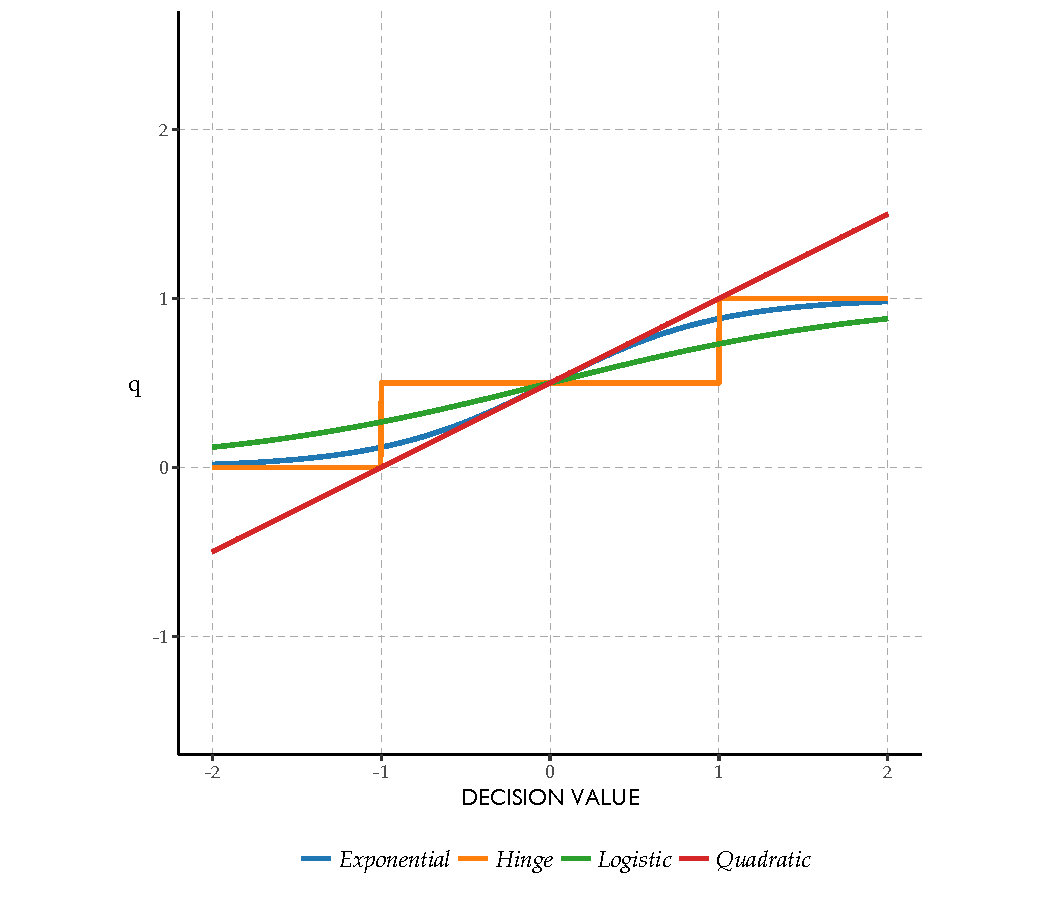
\includegraphics[width=\maxwidth]{figure/responsibilities-1} \caption[For a single unlabeled object, the responsibility that causes a zero gradient of the semi-supervised objects at the supervised solution, for different decision values of the unlabeled object]{For a single unlabeled object, the responsibility that causes a zero gradient of the semi-supervised objects at the supervised solution, for different decision values of the unlabeled object.}\label{figure:responsibilities}
\end{figure}


\end{knitrout}

\subsection{Logistic Loss}

Consider the logistic loss function given by
$$\phi(y \mathbf{x}^\top \mathbf{w})=\log(1+\exp(-y \mathbf{x}^\top \mathbf{w}))\,,$$
and whose minimization leads to the logistic regression classifier. Its derivative is given by
$$\phi^\prime (y\mathbf{x}^\top \mathbf{w}) = \frac{-\exp(-y\mathbf{x}^\top \mathbf{w})}{1+\exp(-y\mathbf{x}^\top \mathbf{w})}\,,$$
from which we can verify it is a monotonically decreasing loss.
Applying Equation~\eqref{eq:solutionq} we find that
\begin{align}
q = & \frac{-\exp(\mathbf{x}^\top \mathbf{w}_\mathrm{sup})}{1+\exp(\mathbf{x}^\top \mathbf{w}_\mathrm{sup})} \nonumber \\
 & \times  \left( \frac{-\exp(-\mathbf{x}^\top \mathbf{w}_\mathrm{sup})}{1+\exp(-\mathbf{x}^\top \mathbf{w}_\mathrm{sup})} + \frac{-\exp(\mathbf{x}^\top \mathbf{w}_\mathrm{sup})}{1+\exp(\mathbf{x}^\top \mathbf{w}_\mathrm{sup})}\right)^{-1} \, . \nonumber
 \end{align}
Because the second term equals $-1$, after rewriting the first term, we have
$$ q = \frac{1}{1+\exp(-\mathbf{x}^\top \mathbf{w}_\mathrm{sup})} \,\, .$$
%This is equal to the class posterior of the positive class, given by the logistic regression model. 
Thus we see that the responsibility assigned to the new object is exactly the class posterior assigned by logistic regression.

\subsection{Support Vector Machine}
The hinge loss, employed in support vector classification, has the form
$$\phi(y\mathbf{x}^\top \mathbf{w})=\max(1-y \mathbf{x}^\top \mathbf{w},0) \, .$$
The value for the derivative at all points except $1-y \mathbf{x}^\top \mathbf{w}=0$ is given by
$$
\phi^\prime (y \mathbf{x}^\top \mathbf{w}) =
\begin{cases}
-1 ,& \text{if } 1-y \mathbf{x}^\top \mathbf{w}>0\\
0,& \text{otherwise} \, .
\end{cases}
$$
Plugging this into Equation~\eqref{eq:solutionq}, we have that
$$
q =
\begin{cases}
    \frac{1}{2} ,& \text{if } -1 < \mathbf{x}^\top \mathbf{w}_\mathrm{sup} < 1\\
    1,              & \text{if } \mathbf{x}^\top \mathbf{w}_\mathrm{sup} > 1 \\
    0 & \text{if } \mathbf{x}^\top \mathbf{w}_\mathrm{sup} < -1 \, .
\end{cases}
$$
If the prediction is strongly positive (respectively, negative), it will be assigned to the positive (negative) class. If on the other hand, it is within the margin, it gets assigned to both classes equally.
It means that for the unlabeled objects in the margin, any change in $\mathbf{x}^\top \mathbf{w}_\mathrm{sup}$ has an opposite contribution for the part of the loss corresponding to the positive and the negative class. Only by weighting the two options equally will a change in $\mathbf{x}^\top \mathbf{w}_\mathrm{sup}$ not yield a change in the loss.

\subsection{Quadratic Loss} \label{section:quadraticloss}
Now consider the quadratic loss, which is a non-monotonically decreasing loss function:
$$\phi(y \mathbf{x}^\top \mathbf{w})=(1-y \mathbf{x}^\top \mathbf{w})^2 \,.$$
Its derivative is
$$\phi^\prime(y \mathbf{x}^\top \mathbf{w}) = - 2 (1-y \mathbf{x}^\top \mathbf{w}) \, .$$
Again using \eqref{eq:solutionq} we find that
$$q = \frac{-2 (1+\mathbf{x}^\top \mathbf{w}_\mathrm{sup})}{-2 (1-\mathbf{x}^\top \mathbf{w}_\mathrm{sup}) -2 (1+\mathbf{x}^\top \mathbf{w}_\mathrm{sup})}$$
which we can simplify to
$$q = \frac{ \mathbf{x}^\top \mathbf{w}_\mathrm{sup} + 1}{2} \,.$$
This is the rescaling of the decision function from the interval $[-1,+1]$ to $[0,1]$. Note that in this case $\mathbf{x}^\top \mathbf{w}$ is not necessarily restricted to be within $[-1,+1]$ and so it may occur that $q \notin [0,1]$. In this case there is no assignment of the responsibilities that recovers the supervised solution and thus the unlabeled data forces us to update the decision function $\mathbf{x}^\top \mathbf{w}$ for the semi-supervised classifier.

When $U>1$, for the monotonically decreasing loss functions, it was enough to show that each $q_i \in [0,1]$ can be set individually in order to reconstruct the supervised solution using a responsibility vector $\mathbf{q} \in [0,1]^U$. For the quadratic loss, however, the situation is more complex when multiple unlabeled objects are available. This is because, considering each $q_i$ individually might not allow us to find  $\mathbf{q} \in [0,1]^U$ for which the gradient of the semi-supervised objective at the supervised solution is equal to zero, but there could still be a combined $\mathbf{q} \in [0,1]^U$ for which this does hold, as we discussed for the general case in Theorem~\ref{eq:possible}.

It turns out that if the dimensionality $d \geq U$, such a $\mathbf{q} \in [0,1]^U$ does not exist as long as
$$\mathbf{X}_\mathrm{u} \mathbf{w}_\mathrm{sup} \notin  [-1,1]^U \, .$$  The proof of this is given in the appendix but is basically a restatement of Theorem~\ref{eq:possible}.  If $d \leq U$, however, then it is also guaranteed that such $\mathbf{q} \in [0,1]^U$ does not exist if
$$\| \mathbf{X}_\mathrm{u} \mathbf{w}_\mathrm{sup} \|_2 > \sqrt{U} \, .$$
This last result is essentially different from Theorem \ref{eq:possible} as it shows that even if some of the unlabeled points are within the margin, the semi-supervised learner has to be different from the supervised learner if one or more of the unlabeled points are sufficiently far outside of the margin. The proof is given in the appendix.

\subsection{Absolute Loss}
The absolute loss is given by
$$\phi(y \mathbf{x}^\top \mathbf{w})=|1-y \mathbf{x}^\top \mathbf{w}| \, .$$
and its derivative at all values except $1-y \mathbf{x}^\top \mathbf{w}=0$ then becomes
$$
\phi^\prime (y \mathbf{x}^\top \mathbf{w}) =
\begin{cases}
-1 ,& \text{if } 1-y \mathbf{x}^\top \mathbf{w}>0\\
+1,& \text{otherwise} \, .
\end{cases}
$$
When $-1 <y \mathbf{x}^\top \mathbf{w}_\mathrm{sup}<1$, we can use Equation~\eqref{eq:solutionq} to find $q=\tfrac{1}{2}$. Otherwise, $\phi'(\mathbf{x}^\top \mathbf{w}_\mathrm{sup}) + \phi'(-\mathbf{x}^\top \mathbf{w}_\mathrm{sup}) = 0$ and there is no $q$ that makes the gradient of the semi-supervised objective in the supervised solution equal to zero. In that case, when we have a single unlabeled object, the semi-supervised solution is an improvement over the supervised solution. For the case of multiple unlabeled objects it may again be possible to find a vector of responsibilities $\mathbf{q} \in [0,1]^U$ that recovers the supervised solution. Again, Theorem~\ref{eq:possible} offers a sufficient condition where the semi-supervised solution must improve over its supervised counterpart.

\section{Discussion}  \label{section:Discussion}
\subsection{Impossibilities of Semi-supervised Learning}
As \citet{Seeger2001} and others have argued, for diagnostic methods, where $p(y|\mathbf{x})$ gets modeled directly and not through modeling the joint distribution $p(y,\mathbf{x})$, it seems semi-supervised learning without additional assumptions should be impossible because the parameters of $p(y|\mathbf{x})$ and $p(y,\mathbf{x})$ are a priori independent. Considering why these methods do not allow for safe semi-supervised versions offers a different understanding of why this may or may not be true.  While our results applied to logistic regression corroborates their claim, the quadratic loss shows a counter example. This shows that for non-monotonically decreasing losses, even safe improvements can be possible in the diagnostic setting. One important strength of our analysis is that we also consider the minimization of loss functions that may not induce a correct probability. It is the monotonic decreasingness of the loss, rather than correspondence to a probabilistic model that determines whether safe semi-supervised learning is possible. Moreover, some of the losses for which safe semi-supervised learning is possible are successfully applied in supervised learning in practice and it is therefore interesting that safe semi-supervised versions exist.

It has also been suggested that the possibility of semi-supervised learning depends on the causal direction of $p_{Y|X}$ \cite{Scholkopf2012}. This seems at odds with our result that pessimistic semi-supervised learning is possible for non-monotonically decreasing losses, regardless of the causal structure of the problem. We think this is again due to the our lack of assumptions that the model that is used is a correctly specified probabilistic model, which is required for the results in \cite{Scholkopf2012} to hold.

Our results also might seem to contradict the result by \citet{Sokolovska2008} that, when the supervised model is misspecified, a particular semi-supervised adaptation of logistic regression has an asymptotic variance that is at least as small as supervised logistic regression. In this work, however, we cover the pessimistic setting where a semi-supervised learner needs to outperform the supervised learner for all possible labelings in a finite sample setting. This is a much stricter requirement than the asymptotic result in \citep{Sokolovska2008}. Moreover, we do not require the supervised model to be misspecified. 
For semi-supervised learning in general, their result is encouraging, while for safe semi-supervised learning it makes sense to consider the results in the pessimistic setting.

The (negative) result presented here is in line with the conclusions of \citet{Ben-David2008}, who show that the worst-case sample complexity of a supervised learner is at most a constant factor higher than that of any semi-supervised approach for a classifier over the real line, and they conjecture this result holds in general. \citet{Darnstadt2013} prove that a slightly altered and more precise formulation of this conjecture holds when hypothesis classes have finite VC-dimension, while they show that it does not hold for more complex hypothesis classes. Whereas these works consider generalization bounds on the error rate in the PAC learning framework, in our work, we considered a more conservative or pessimistic setting of safe semi-supervised learning, while considering performance on a finite sample in terms of the surrogate loss. This leads to an alternative explanation why these (strict) improvements are not possible for some losses, similar to the claim in \citet{Ben-David2008}. It also leads, however, to the contrasting conclusion that for some losses, these improvements are possible (even when the VC dimension is finite), which contradicts the claim of \citet{Ben-David2008} that improvements are not possible unless strong assumptions about the distribution of the labels are made.

\subsection{Safe Semi-supervised Learning}
What do our results mean for purportedly safe approaches to semi-supervised learning, such as those proposed in \citep{Li2015} and \citep{Kawakita2014a}? The results by \citet{Kawakita2014a} show their proposed procedure is asymptotically safe, similar to the results by \citet{Sokolovska2008}, but under weaker assumptions. In our analysis, we consider performance on the limited set of labeled and unlabeled objects. For monotonically decreasing margin-based losses, it may still be possible to find a procedure that outperforms supervised learning in expectation, but not on a particular set of objects for all its labelings.

The improvement guarantee, in terms of classification accuracy, of the safe semi-supervised SVM by \citet{Li2015} depends on the assumption that the true labeling of the objects is given by one of the low-density separators that their algorithm finds. An advantage of our analysis is that we avoid making such untestable assumptions. The consequence of this is that all possible labelings have to be considered, not just those corresponding to a low-density separator. If their low-density assumptions holds, their method provides one way of making use of this information to guarantee safe improvements. As we have demonstrated, however, in a worst case sense no such guarantees can be given, at least in terms of the semi-supervised objective considered in our work. Without making these untestable assumptions, our results show a safe semi-supervised support vector machine is impossible.

\subsection{Consequences and Opportunities}
The results of Theorem~\ref{theorem:hardlabels} and Theorem~\ref{theorem:softlabels} show that for many well-known losses that are monotonically decreasing, it is impossible to construct a safe semi-supervised method that is guaranteed to not lead to worse performance than the supervised solution, without making additional assumptions. In this way, these results offer a different perspective on why this type of semi-supervised learning is not possible for some losses, by indicating the monotonic decreasingness property as essential to the proofs.

One consequence of these results is that if we want to construct semi-supervised learners with the type of guarantee studied here, we need more constraints than those given by the pessimistic approach, to reduce the size of the set of possible label assignments that is considered. For unlabeled data to be helpful, we need additional constraints on the semi-supervised solution coming from substantive assumptions, like a low-density or clustering assumption. We need to keep in mind that these strong assumptions, however, might have also helped improve the supervised solution, without considering the unlabeled data, and properly compare any improvements of the semi-supervised learner to a supervised learner that also takes these assumptions into account.

For the non-monotonically decreasing loss functions, safe improvement is possible. One could ascribe this fact to a peculiar property of these losses: they give increasingly higher loss even if the sign of the decision function is correct. The improvements in terms of the loss that we get may therefore not be useful for classification, since they may be in a part of the loss function where the surrogate loss already forms a bad approximation to the $\{0,1\}$-loss. In the supervised case, however, surrogate losses like the quadratic loss generally give decent performance in terms of the error rate. In some sense it is therefore not surprising that its pessimistic semi-supervised counterpart has also shown increased performance as more unlabeled data is added to the training set \citep{Krijthe2017}.

Our analysis takes a rather extreme view of what is required to be safe, where the semi-supervised learner has to outperform the supervised learner on every possible dataset. A less strict notion of safety might consider this improvement to hold in expectation over datasets or labelings, rather than for a particular dataset. On any one particular dataset that a practitioner is faced with, however, the unlabeled data may then cause a decrease in the performance compared to the supervised classifier.
% 
% <<responsibilities, echo=FALSE, fig.cap="For a single unlabeled object, the responsibility that causes a zero gradient of the semi-supervised objects at the supervised solution, for different decision values of the unlabeled object.", fig.lp='figure:', fig.height=3,fig.width=6, warning=FALSE, message=FALSE,cache=TRUE >>=
% objectives <- list(
%   "Decision Value" = function(o) {o},
%   "Quadratic" = function(o) {(o+1/2)},
%   "Logistic" = function(o) {1/(1+exp(-o))},
%   "Hinge" = function(o) { sapply(o,function(x) {if(x>1) 1 else if(x < -1) 0 else 0.5}) },
%   "Exponential" = function(o) { exp(o)/(exp(-o)+exp(o)) }
% )
% 
% lapply(objectives, function(f) f(seq(-2,2,length.out=1000))) %>%
%   as_data_frame %>%
%   gather(Loss,Value,-`Decision Value`) %>%
%   ggplot(aes(x=`Decision Value`,y=Value,color=Loss)) +
%   geom_line(size=1) +
% 
%   theme_minimal() +
%   ylab("q") +
%   theme(text=element_text(family="Palatino"), axis.title.y=element_text(angle=0),axis.title=element_text(size=10)) +
%   coord_equal()
% @

\section{Conclusion}
We have shown that for the class of convex margin-based losses, the fact whether they are monotonically decreasing or not plays a key role in whether they admit safe semi-supervised procedures. In particular, we have shown that, without making additional assumptions, it is impossible to construct safe semi-supervised procedures for monotonically decreasing losses by deriving what partial assignment of the unlabeled objects leads to the recovery of the supervised classifier from a semi-supervised objective. This subsequently implied that if we choose any semi-supervised procedure that deviates from the supervised solution, there is some labeling of the unlabeled objects (which could be the true labeling) for which it decreases performance. While this means that for many supervised procedures it is impossible to construct a safe semi-supervised learner in this strict sense, some losses do admit such solutions. 
A less strict guarantee might admit performance improvement by aiming for semi-supervised solutions that in expectation rather than on any particular dataset, outperform their supervised counterparts. 

The stark reality is that if one sticks to strictly safe semi-supervised learning, beside opportunities for some surrogate losses, there are clear limits to the development of such procedures.  It is this reality that we have characterized.

\section*{Acknowledgements}

We thank Alexander Mey for his constructive feedback to an earlier version of this chapter.

\section*{Appendix}
%\section{Multiple objects for the quadratic loss}
%\begin{proof}
Whether it is possible to find some $\mathbf{q}$ for which minimizing the semi-supervised objective gives the supervised solution in case of the quadratic loss comes down to the question whether the system of equations
\begin{equation} \label{conditionquadratic}
\mathbf{X}_\mathrm{u} ^\top \mathbf{q} = \frac{1}{2} ( \mathbf{X}_\mathrm{u}^\top \mathbf{1} + \mathbf{X}_\mathrm{u}^\top \mathbf{X}_\mathrm{u} \mathbf{w}_\mathrm{sup} )
\end{equation}
has a solution $\mathbf{q} \in [0,1]^U$.
% Its solutions are given by
% $$\mathbf{q} = \frac{1}{2} (\mathbf{X}_\mathrm{u}^\top)^+ \mathbf{X}_\mathrm{u}^\top \mathbf{1} + (\mathbf{X}_\mathrm{u}^\top)^+ \mathbf{X}_\mathrm{u}^\top \mathbf{X}_\mathrm{u} \mathbf{w}_\mathrm{sup} + (I - (\mathbf{X}_\mathrm{u}^\top)^+ \mathbf{X}_\mathrm{u}^\top) \mathbf{v}$$
%$\mathbf{v} \in \mathcal{R}^U$.
Let $(\mathbf{X}_\mathrm{u}^\top)^+$ denote the Moore-Penrose pseudo-inverse of $\mathbf{X}_\mathrm{u}^\top$. We consider two scenarios: $d \geq U$, the number of unlabeled objects is smaller or equal to the dimensionality of the feature vectors, and $d \leq U$, where we have more unlabeled objects than dimensions.

If $d \geq U$, the pseudo-inverse can be written as $(\mathbf{X}_\mathrm{u} \mathbf{X}_\mathrm{u}^\top)^{-1} \mathbf{X}_\mathrm{u}$ meaning we have a unique solution
$$
\mathbf{q} = \frac{1}{2} (\mathbf{1} + \mathbf{X}_\mathrm{u} \mathbf{w}_\mathrm{sup})
$$
and so the supervised solution cannot be recovered unless $\mathbf{X}_\mathrm{u} \mathbf{w}_\mathrm{sup} \in [-1,1]^U$.

If $d \leq U$, the pseudo-inverse can be written as $(\mathbf{X}_\mathrm{u}^\top)^+ = \mathbf{X}_\mathrm{u} (\mathbf{X}_\mathrm{u}^\top \mathbf{X}_\mathrm{u})^{-1}$. Rewriting Equation~\eqref{conditionquadratic} in terms of $\mathbf{r} = 2\mathbf{q}-1$, the condition for improvement is that
$$\mathbf{X}_\mathrm{u} ^\top \mathbf{r} = \mathbf{X}_\mathrm{u}^\top \mathbf{X}_\mathrm{u} \mathbf{w}_\mathrm{sup} $$
has no solution $\mathbf{r} \in [-1,1]^U$. Solving this using the pseudo-inverse we find the solution $\mathbf{r}^+$ with the smallest norm among all possible solutions:
$$\mathbf{r}^+ = \mathbf{X}_\mathrm{u} \mathbf{w}_\mathrm{sup} \, .$$
We therefore have for any solution $\mathbf{r}$ that 
$$\| \mathbf{r} \|_2 \ge \| \mathbf{X}_\mathrm{u} \mathbf{w}_\mathrm{sup} \|_2$$
and so if $\| \mathbf{X}_\mathrm{u} \mathbf{w}_\mathrm{sup} \|_2 > \sqrt{U}$, this implies that every solution $\mathbf{r}$ lies outside of the unit cube $[-1,1]^U$ and no proper solution of responsibilities exists.
%\end{proof}

% Suppose $\| \mathbf{X}_\mathrm{u} \mathbf{w}_\mathrm{sup} \|_2>\sqrt{U}$, we have:
%$$\| \mathbf{r} \|_2 > \| \mathbf{X}_\mathrm{u} \mathbf{w}_\mathrm{sup} \|_2>\sqrt{U} \, . $$
%for all solutions $\mathbf{r}$. Since for all $\mathbf{r} \in [-1,1]^U$ we have $\| \mathbf{r}\|_2<\sqrt{U}$ there is no $\mathbf{r} \in %[-1,1]^U$ that is a solution of \eqref{conditionquadratic}.

%
% So if $\mathbf{H} = \mathbf{X}_\mathrm{u} (\mathbf{X}_\mathrm{u}^\top \mathbf{X}_\mathrm{u})^{-1} \mathbf{X}_\mathrm{u}$ denotes the hat matrix we have
% $$
% \mathbf{q} = \frac{1}{2} (\mathbf{H} \mathbf{1} + \mathbf{X}_\mathrm{u} \mathbf{w}_\mathrm{sup}) + (I - \mathbf{H}) \mathbf{v} \, .
% $$
% Assuming $\mathbf{X}$ contains an intercept and since $\mathbf{H} \mathbf{X} = \mathbf{X}$
% $$
% \mathbf{q} = \frac{1}{2} (\mathbf{1} + \mathbf{X}_\mathrm{u} \mathbf{w}_\mathrm{sup}) + (I - \mathbf{H}) \mathbf{v} \, .
% $$


\chapter[Optimistic Semi-supervised Least Squares Classification]{Optimistic Semi-supervised\\Least Squares Classification}
\chaptermark{Optimistic Least Squares}
\label{chapter:optimistic}
\blfootnote{This chapter appeared as: Krijthe, J. H., \& Loog, M. 2016. Optimistic Semi-supervised Least Squares Classification. In Proceedings of the 23rd International Conference on Pattern Recognition (pp. 1677–1682).}


\begin{abstract}
The goal of semi-supervised learning is to improve supervised classifiers by using additional unlabeled training examples. In this work we study a simple self-learning approach to semi-supervised learning applied to the least squares classifier. We show that a soft-label and a hard-label variant of self-learning can be derived by applying block coordinate descent to two related but slightly different objective functions. The resulting soft-label approach is related to an idea about dealing with missing data that dates back to the 1930s. We show that the soft-label variant typically outperforms the hard-label variant on benchmark datasets and partially explain this behaviour by studying the relative difficulty of finding good local minima for the corresponding objective functions.
\end{abstract}

\section{Introduction}
Semi-supervised learning aims to improve supervised classifiers by incorporating abundant unlabeled training examples in the training of a classifier. Many approaches to semi-supervised learning have been suggested (for one overview see \citet{Chapelle2006}), mostly taking advantage of assumptions that allow information about the distribution of the feature values to inform decisions as to what constitutes a good classifier.

Instead of introducing yet another assumption to the literature, the goal of this work is to revisit a classic approach to semi-supervised learning to incorporate unlabeled data in the training of the least squares classifier: self-learning. While self-learning is often proposed as an ad hoc procedure, we properly formulate it as the minimizer of a particular objective function in the least squares setting. A slightly different formulation then leads to a new type of soft-label self-learning. 

This soft-label self-learning procedure is closely related to a procedure that dates all the way back to an approach to missing data in least squares regression by \citet{Yates1933} and \citet{Healy1956} from the 1930s and 1950s respectively. We revisit these ideas in the context of the present paper.

In a set of experiments, we show that the soft-label self-learning variant tends to outperform the hard-label variant. We explain this behaviour based on the differing difficulty of finding good local minima of the corresponding objective functions. 

The paper is structured as follows: we will first explain how our ideas relate to early approaches to deal with missing data in statistics and to the well known self-learning and expectation maximization (EM) approaches to semi-supervised learning. Afterwards we will formulate two different objective functions for the semi-supervised least squares classification problem. We show that applying block coordinate descent \cite[Ch. 2.7]{Bertsekas1999} to these objective functions corresponds to either hard-label, respectively soft-label self-learning. We then study the properties of these objective functions using some simulation studies and end with a set of experiments on benchmark datasets that shows that soft-label self-learning tends to outperform the hard-label variant.

\section{Historical Perspective}

\subsection{Self-learning and EM}
Arguably, the most simple and straightforward approach to semi-supervised learning is a procedure known as self-learning. Starting with the supervised classifier trained using only labeled data, one predicts the labels for the unlabeled objects and uses these in the next iteration of training the classifier. This is done until the predicted labels of the unlabeled objects no longer change. Self-learning was introduced in \citet{McLachlan1975} and \citet{McLachlan1977} as a more feasible alternative to the proposal by \citet{Hartley1968b} to consider all possible labelings of the unlabeled data and find the one that minimizes the log likelihood of an ANOVA model.

For probabilistic models, such as linear discriminant analysis based on a Gaussian model of each class, a closely related approach to self-learning is to apply the Expectation Maximization (EM) procedure \citep{Dempster1977} that attempts to find the parameters that maximize the likelihood  of the model after marginalizing out the unknown labels. This leads to an algorithm where in each iteration, the parameters of the model are estimated based on the current partial assignment of objects to different classes (the maximization step), after which these assignments are updated based on the new model parameters (the expectation step). The assignments of unlabeled objects to classes in each stage is a partial assignment based on the posterior probability given by the current parameter estimates of the model, rather than a hard assignment to a single class as is typically used in self-learning.

\subsection{Connection to Missing Data in Regression}
In this work we consider the least squares classifier, the classifier that minimizes the squared error of the fit of a (linear) decision function to the class labels encoded as $\{0,1\}$ \cite[p.103]{Hastie2009}. While the classifier in this form does not have a proper likelihood function to which we can apply the EM procedure, it is closely related to least squares regression where \citet{Healy1956} proposed a similar iterative procedure. The idea behind this iterative procedure dates back as early as 1933 to work by \citet{Yates1933}. Yates noted that one can get unbiased estimates of the regression parameters when outcomes are missing by plugging in the regression estimates for the missing values that were given by the complete data alone. The problem is how to find these regression estimates. While for some regression designs analytical solutions exist \cite{Wilkinson1958} to fill in the missing values, \citet{Healy1956} describes the simple approach of starting with random values and iteratively updating the regression parameters and setting the missing values to the values predicted by the updated model.
They prove this procedure reduces the residual sum of squares at each iteration. It was later shown \cite{Dempster1977} that for the linear regression model with Gaussian errors, this procedure corresponds to the EM algorithm.

Note that the goal of these procedures is to deal with missing values in a convenient automatic way, not necessarily to improve the estimator \cite[Ch. 2]{Little2002}, as is the case in semi-supervised learning.

% Preece builds upon this work by suggesting larger updates of the missing values in each iteration to speed up convergence. This is based on the observation that the procedure proposed by Yates for a single missing value uses a larger update than the simple scheme by Healy and Westmacott. 

Unlike in the regression setting, in least squares classification, we know that the true labels are not values in $\mathbb{R}$ but rather restricted to $\{0,1\}$, or as we will consider, $[0,1]$. We will show that the iterative approach of \citet{Healy1956}, when taking into account the constraints that missing outcomes are $[0,1]$ can be formulated as a block coordinate descent procedure on the quadratic loss function and that, in fact, an improved classifier can generally be obtained by using this procedure. For a different take on how to introduce soft-labels in self-learning and how this relates to EM, see \citet{Mey2016}.

\subsection{Pessimism vs. Optimism}
To guard against unlabeled data leading to worse classifiers one can attempt to construct a classifier that improves over the supervised classifier even for the worst possible labeling of the unlabeled objects, which is proposed in contrastive pessimistic learning, see \citet{Loog2016} and \citet{Krijthe2015}. This is the pessimistic approach to semi-supervised learning. In contrast, we refer to the approaches studied here as optimistic approaches, where in each step of the algorithm, we consider the best-case labels, rather than the worst-case labels.

\section{Regularized Least Squares Classification}
Let $\mathbf{x}$ denote a $d\times 1$ feature vector, potentially containing a constant feature encoding the intercept.
$\mathbf{X}$ is the $L \times d$ design matrix of the labeled examples, while $\mathbf{X}_\text{u}$ is the  $U \times d$ design matrix of the unlabeled examples. $\mathbf{y}$ is the $L\times 1$ vector containing the labels encoded as $\{0,1\}$.
$\mathbf{w}$ denotes the weight vector of a linear classifier.

In the supervised setting, the binary regularized least squares classifier is defined by the following loss function:
\begin{equation}
J_s(\mathbf{w}) = \sum_{i=1}^L (\mathbf{x}_i^\top \mathbf{w}-y_i)^2 + \lambda \|\mathbf{w} \|^2 \,. \label{eq:supervisedobjective}
\end{equation}
The minimizer of this objective function has a well-known closed form solution:
\begin{equation}
\mathbf{w} = \left( \mathbf{X}^\top \mathbf{X}  + \lambda \mathbf{I} \right)^{-1} \mathbf{X}^\top \mathbf{y} \,. \label{eq:olssolution}
\end{equation}
To label a new object a threshold is typically set at $\tfrac{1}{2}$:
$$
c_\mathbf{w}(\mathbf{x}) = 
\begin{cases}
    1, & \mathbf{x}^\top \mathbf{w}>\tfrac{1}{2}\\
    0,              & \text{otherwise}
\end{cases}
$$

\section{Optimistic Semi-supervised LSC}

\begin{knitrout}
\definecolor{shadecolor}{rgb}{1, 1, 1}\color{fgcolor}\begin{figure}
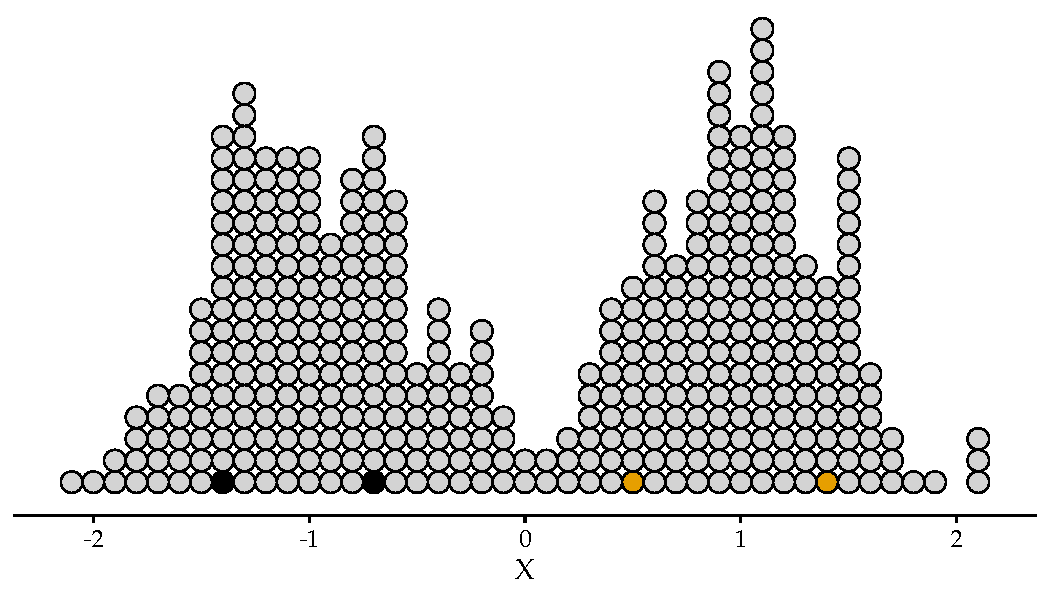
\includegraphics[width=\maxwidth]{figure/attractionexample-1} \caption[Dotplot of example dataset with 4 labeled objects and 396 unlabeled objects]{Dotplot of example dataset with 4 labeled objects and 396 unlabeled objects.}\label{fig:attractionexample}
\end{figure}


\end{knitrout}

We present two closely related ways to extend the supervised least squares objective function to include unlabeled data in an optimistic way. We refer to the first formulation as the label based formulation and show that applying a block coordinate descent procedure to this objective function corresponds to a type of soft-label self-learning, similar to Expectation Maximization. The second formulation is a very similar responsibility based formulation where a block coordinate descent approach corresponds to the familiar hard-label self-learning.

\subsection{Label Based Formulation}
A straightforward way to include the unlabeled objects into the objective function \eqref{eq:supervisedobjective} is to introduce a variable for the missing labels $\mathbf{u}$ and then use the supervised objective function as if we knew these labels:
$$
J_l(\mathbf{w},\mathbf{u}) = \| \Xe \mathbf{w}-\begin{bmatrix} \mathbf{y} \\ \mathbf{u} \end{bmatrix} \|^2 + \lambda \|\mathbf{w} \|^2
$$
where $\Xe$ is the concatenation of $\mathbf{X}$ and $\mathbf{X}_\text{u}$. Since we do not know $\mathbf{u}$, one possibility is to minimize over both $\mathbf{w}$ and $\mathbf{u}$:
$$
\min_{\mathbf{w}\in \mathbb{R}^d,\mathbf{\mathbf{u} \in [0,1]^U}} J_l(\mathbf{w},\mathbf{u}) \,.
$$
Taking the gradient with respect to $\mathbf{w}$ and setting it equal to zero gives
$$
\mathbf{w} = \left( \mathbf{X}_\text{e}^\top \mathbf{X}_\text{e}  + \lambda \mathbf{I} \right)^{-1} \mathbf{X}_\text{e}^\top \mathbf{y}_\text{e} \,.
$$
% $$
% \frac{\nabla J_l(\mathbf{w},\mathbf{u})}{\nabla \mathbf{w}} = 2 \mathbf{X}_\text{e}^\top \mathbf{X}_\text{e} \mathbf{w} - 2 \mathbf{X}_\text{e}^\top \mathbf{y}_\text{e} + 2 \lambda \mathbf{w}
% $$
% $$
% \frac{\nabla J_l(\mathbf{w},\mathbf{u})}{\nabla \mathbf{w}} = 2 \mathbf{X}_\text{e}^\top \mathbf{X}_\text{e} \mathbf{w} - 2 \mathbf{X}_\text{e}^\top \mathbf{y}_\text{e} + 2 \lambda \mathbf{w}
% $$
where $\mathbf{y}_\text{e}=\begin{bmatrix} \mathbf{y} \\ \mathbf{u} \end{bmatrix}$. So given a choice of labels $\mathbf{u}$ for the unlabeled objects, this naturally has the same form as the solution \eqref{eq:olssolution} in the supervised setting.

The gradient with respect to the unknown labels is:
$$
\frac{\nabla J_l(\mathbf{w},\mathbf{u})}{\nabla \mathbf{u}} = -2 (\mathbf{X}_\text{u} \mathbf{w} - \mathbf{u})
$$
so given a set of weights, $\mathbf{w}$, the minimizing labeling is 
$$\mathbf{u} = \mathbf{X}_\text{u} \mathbf{w} \,.$$
Taking into account, however, the constraint that $\mathbf{u} \in [0,1]^U$, the solution is to project each label onto $[0,1]$:
$$
u_i = 
\begin{cases}
0, & \text{if } \mathbf{x}_i^\top \mathbf{w} < 0\\
\mathbf{x}_i^\top \mathbf{w}, & \text{if } 0 < \mathbf{x}_i^\top \mathbf{w} < 1\\
1, & \text{if } \mathbf{x}_i^\top \mathbf{w} > 1
\end{cases}
$$
In this formulation, for a given $\mathbf{w}$ we get hard labelings whenever the decision function gives a value outside $(0,1)$, but a soft assignment, between $(0,1)$, if it does not.


\begin{knitrout}
\definecolor{shadecolor}{rgb}{1, 1, 1}\color{fgcolor}\begin{figure*}
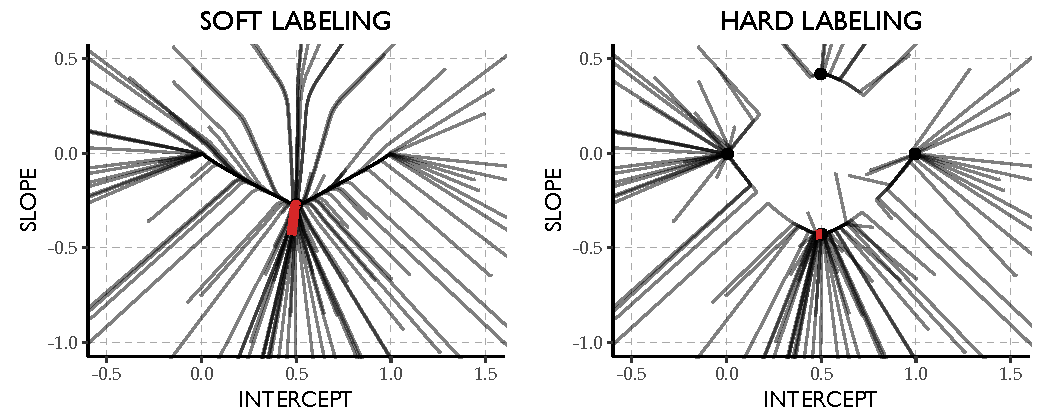
\includegraphics[width=\maxwidth]{figure/attraction1d-1} \caption{Convergence paths of the block coordinate descent procedure for different starting values for the label based objective function (left) and responsibility based objective function (right). Shown are the weights corresponding to the intercept and single feature of a classifier applied to the problem shown in Figure \ref{fig:attractionexample}. Shown in red is the optimization path starting with the supervised solution.}\label{fig:attraction1d}
\end{figure*}


\end{knitrout}


\subsection{Responsibility Based Formulation}
A different way to include the unlabeled data is by introducing a variable $\mathbf{q} \in [0,1]^U$ that indicates what portion of the loss of the two classes should be attributed to the loss for each unlabeled object. We refer to this $\mathbf{q}$ as a vector of responsibilities. While the responsibility is closely related to soft-labels in the previous section, it leads to a slightly different loss function. For generality, let $m$ be the numerical encoding used for one class and $n$ for the other. In this work, we shall use $m=1$ and $n=0$. The objective function becomes:
\begin{align}
J_r(\mathbf{w},\mathbf{q}) = & \| \mathbf{X} \mathbf{w}-\mathbf{y} \|^2 + \lambda \|\mathbf{w} \|^2 \nonumber \\
& + \sum_{i=1}^{U}  q_i (\mathbf{x}_i^\top \mathbf{w} - m)^2  + (1-q_i) (\mathbf{x}_i^\top \mathbf{w} - n)^2 \,. \nonumber \\ \nonumber
\end{align}
Now to solve $\min_{\mathbf{w} \in \mathbb{R}^d, \mathbf{\mathbf{q} \in [0,1]^U}} J_r(\mathbf{w},\mathbf{q})$ we again consider the gradients
$$
\frac{\nabla J_r}{\nabla \mathbf{w}} = 2 \mathbf{X}^\top_\text{e} \mathbf{X}_\text{e} \mathbf{w} - 2 \mathbf{X}^\top \mathbf{y}  - 2 \mathbf{X}_\text{u} (\mathbf{q} m - \mathbf{q} n + n ) + 2 \lambda \mathbf{w}
$$
and
$$
\frac{\nabla J_r}{\nabla q_i} = m^2 - n^2 - 2 (m-n) \mathbf{x}_i^\top \mathbf{w} \,.
$$
More specifically, in the encoding used here:
$$
\frac{\nabla J_r}{\nabla q_i} = - 2 (\mathbf{x}_i^\top \mathbf{w}-0.5) \,.
$$
If the responsibilities are fixed, this objective function leads to the same solution as the label based objective. Unlike for the label based objective, the objective function is now linear in the responsibilities. Minimizing the responsibilities for a given $\mathbf{w}$ leads to setting $q_i=1$ if  $\mathbf{x}_i^\top \mathbf{w}>0.5$ and $q_i=0$ if $\mathbf{x}_i^\top \mathbf{w}<0.5$

Unlike in the previous approach, the optimal procedure becomes to assign hard labelings to each object when $\mathbf{w}$ is kept fixed.

\section{Optimization}
A straightforward approach to find a local minimum of these functions is to use a block coordinate descend procedure where we iteratively 1) update $\mathbf{w}$, using the closed form solution given while keeping the labels/responsibilities fixed and 2) update $\mathbf{u}$ or $\mathbf{q}$ by the updates derived in the previous section. This leads respectively to a soft-label self-learning and hard-label self-learning procedure.

The convergence of these procedures can be verified by the same argument that was used by \citet{Healy1956}: both steps are guaranteed to decrease the value of the objective function.

While this may seem like a naive approach, block-coordinate descent is the bread and butter of semi-supervised learning approaches. We see this in the EM algorithm, which iteratively updates the responsibilities and the model parameters. But even the seemingly unrelated Transductive SVM \cite{Joachims1999}, in its algorithm iteratively updates imputed labels and the decision function to converge to a local optimum of its objective function.

\section{Difficulty of the Optimization Problem}
A nice property of the supervised least squares objective function is that it is convex and allows for a simple closed-form solution. To study the convexity of the semi-supervised extensions of this loss function, we check whether their Hessians are positive semi-definite matrices. The Hessian of the label based extension is given by:
$$
H=\begin{bmatrix} 
2 \mathbf{X}_\text{e}^\top \mathbf{X}_\text{e} & 
-2 \mathbf{X}_\text{u}^\top \\
-2 \mathbf{X}_\text{u} &
-2 \mathbf{I}
\end{bmatrix} \,,
$$
which is not positive semi-definite as it has negative values on its diagonal.
% so for the problem to be convex we would need:
% $$
% 2 \mathbf{z}^\top_1 \mathbf{X}_\text{e}^\top \mathbf{X}_\text{e} \mathbf{z}_1 - 2 \mathbf{z}_2^\top \mathbf{X}_\text{u} \mathbf{z}_1 -2 \mathbf{z}_2^\top \mathbf{I} \mathbf{z}_2  \geq 0 \,.
% $$
% For all $\mathbf{z} \in \mathbb{R}^{d+U}$. Let $\mathbf{z}_1 \in \mathbb{R}^{d}$ be the first $d$ elements in $\mathbf{z}$ and $\mathbf{z}_2 \in \mathbb{R}^{U}$ the remaining $U$ elements. With $\mathbf{z}_1=\mathbf{0}$ and $\mathbf{z}_2 \neq \mathbf{0}$, we have an example where the constraint is violated, showing the function is not convex.

For the responsibility based loss function, the Hessian is slightly different:
% \begin{align}
% \frac{\nabla J}{\nabla \mathbf{q} \nabla \mathbf{q}} = & \mathbf{0} \\
% \frac{\nabla J}{\nabla \mathbf{w} \nabla \mathbf{w}} = & 2 \mathbf{X}_\text{e}^\top \mathbf{X}_\text{e} \\
% \frac{\nabla J}{\nabla \mathbf{w} \nabla \mathbf{u}} = & -2 (m-n) \mathbf{X}_\text{u} \\
% \end{align}
$$
H=\begin{bmatrix} 
2 \mathbf{X}_\text{e}^\top \mathbf{X}_\text{e} & 
-2 (m-n)\mathbf{X}_\text{u}^\top \\
-2 (m-n) \mathbf{X}_\text{u} &
\mathbf{0}
\end{bmatrix} \,.
$$
So for the problem to be convex we would need:
$$
2 \mathbf{z}^\top_1 \mathbf{X}_\text{e}^\top \mathbf{X}_\text{e} \mathbf{z}_1 - 2 (m-n)  \mathbf{z}_2^\top \mathbf{X}_\text{u} \mathbf{z}_1 \geq 0
$$  
for all $\mathbf{z}_1 \in \mathbb{R}^{d}$ and $\mathbf{z}_2 \in \mathbb{R}^{U}$ . When $\mathbf{X}_\text{u}\neq 0$ and $\mathbf{z}_1\neq 0$  it is always possible to pick some $\mathbf{z}_2$ such that the constraint does not hold, so this function is typically not convex either.

Similar to EM-based approaches, we lose convexity for both semi-supervised extensions. One of the extensions may still be easier to optimize than the other. We illustrate the difference between the two objective functions by applying both approaches to the simple dataset shown in Figure~\ref{fig:attractionexample}. We randomly generate $100$ starting values around the supervised solution and plot the convergence of the block coordinate descent procedure for both algorithms in Figure~\ref{fig:attraction1d}. The red line indicates the path of solution when starting at the supervised solution. For the soft-label objective, all starting values converge to the same optimum, while for the hard-label approach, the algorithm converges to four different optima, corresponding to assigning all objects to one of the classes and the two assignments of the clusters to the different classes.

\section{Experiments \& Results}

\subsection{Why Soft-labeling can Lead to Improved Predictions}
For hard self-labeling, it is clear why the semi-supervised solution will generally be different from the supervised procedure: for a lot of classifiers it is unlikely that the minimizer of the loss after assigning labels to the unlabeled objects is going to be exactly the same as the minimizer of the loss on the supervised objects. In the soft-label case, it is less clear: because the labeling is more fine-grained, it may be possible to find some assignment of the labels such that the loss does not change. Figure~\ref{fig:simple-example} illustrates when an update of the classifier occurs: starting with the supervised decision function (solid line), we can set the label of the unlabeled object on the left to $0$, such that its contribution to the loss function is $0$. For the object on the right, however, the best we can do is setting the label to $1$. In the next step, the classifier is updated, after which the labels are updated again. This time, the optimal labeling for the right object is again 1, while the optimum for the left object has now changed due to the updated decision function. The effect is that even as the changes are brought about by objects that have decision values greater than $1$ or smaller than $0$, updates lead to a weight vector that has not only changed in magnitude, but the location of the decision boundary has also shifted based on the configuration of the unlabeled objects.

\begin{knitrout}
\definecolor{shadecolor}{rgb}{1, 1, 1}\color{fgcolor}\begin{figure}
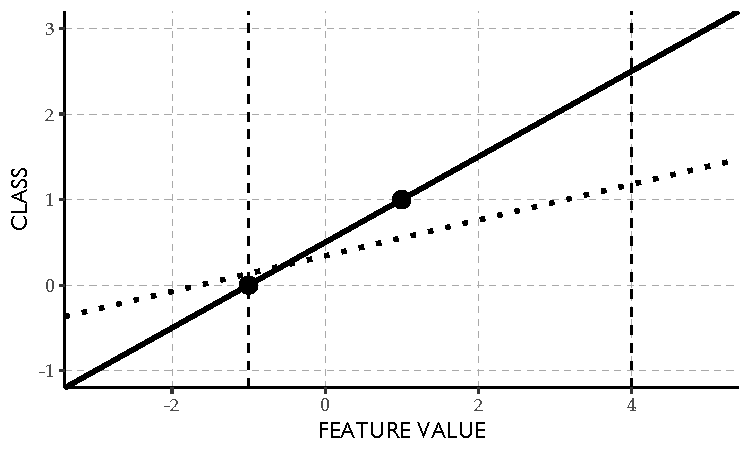
\includegraphics[width=\maxwidth]{figure/simple-example-1} \caption[Example of the first step of soft-label self-learning]{Example of the first step of soft-label self-learning. The circles indicate two labeled objects, while the dashed vertical lines indicate the location of two unlabeled objects. The solid line is the supervised decision function. The dotted line indicates the updated decision function after finding soft labels that minimize the loss of the supervised solution and using these labels as the labels for the unlabeled data in the next iteration.}\label{fig:simple-example}
\end{figure}


\end{knitrout}
 
\begin{knitrout}
\definecolor{shadecolor}{rgb}{1, 1, 1}\color{fgcolor}\begin{figure}
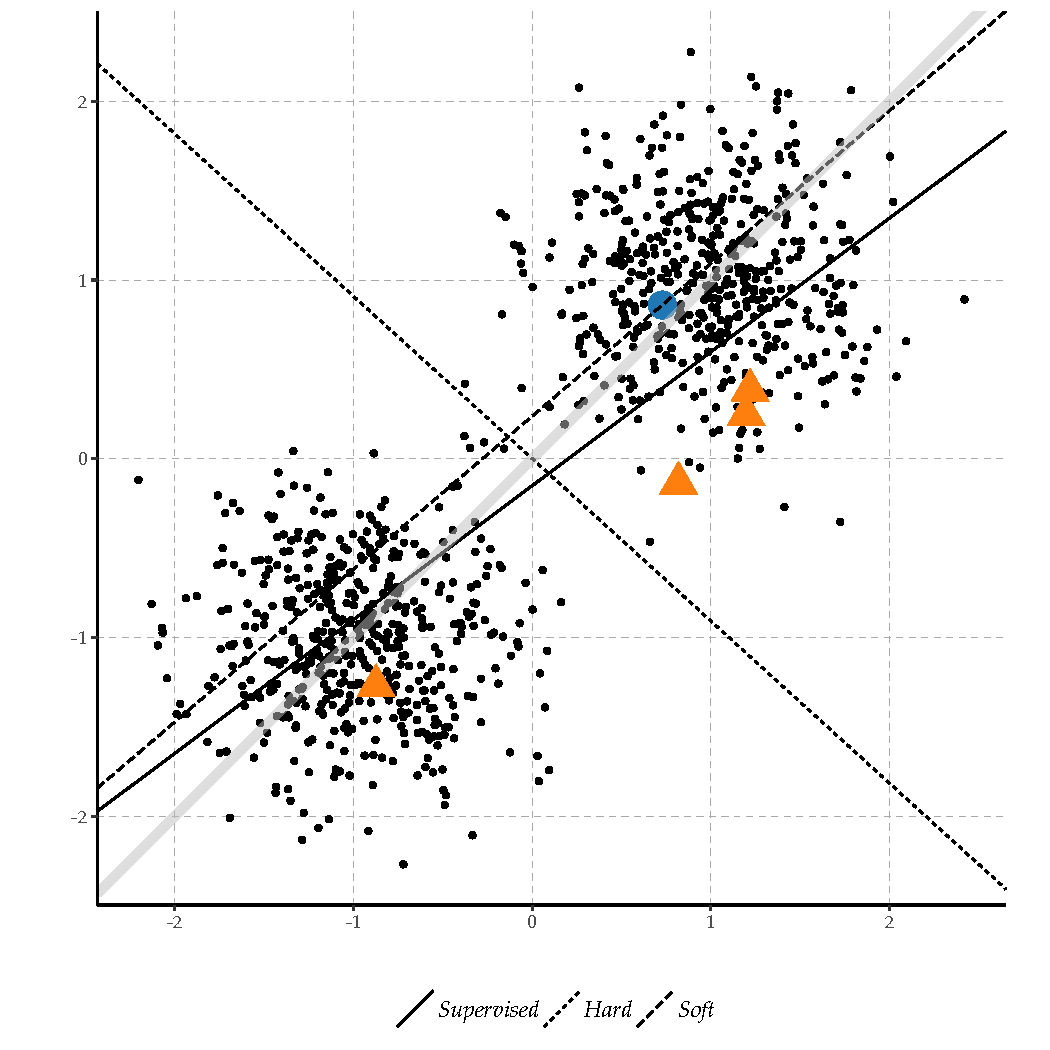
\includegraphics[width=\maxwidth]{figure/example-1} \caption[Example where hard-label self-learning decreases classification performance compared to the supervised solution, while comparable performance to the supervised solution is obtained by soft-label self-learning]{Example where hard-label self-learning decreases classification performance compared to the supervised solution, while comparable performance to the supervised solution is obtained by soft-label self-learning. Light-grey line indicates true decision boundary.}\label{fig:example}
\end{figure}


\end{knitrout}


\subsection{Why Hard-labeling Might Fail}
While Figure~\ref{fig:attraction1d} indicated that the hard-label approach can more easily get stuck in a bad local optimum, using the supervised solution as the initialization leads to a reasonable solution. Figure~\ref{fig:example} shows an example where this is not the case, and the hard-label approach leads away from the reasonable supervised solution to one that has worse performance. The soft-label procedure, on the other hand, gives a classifier that is similar to the supervised procedure.

\subsection{Local Optima}
One might wonder how often these bad local minima occur on benchmark datasets. We take a set of $16$ well-known datasets from \citet{Chapelle2006} and the UCI repository \citep{Lichman2013}. Figure~\ref{fig:localoptima} shows the classification performance of the solutions the algorithms converge to for several random initialization of the algorithm and when the algorithms are initialized using the supervised solution. For each dataset, we randomly assign $20\%$ of the objects to the test set, and randomly remove labels from $80\%$ of the remaining objects. We randomly initialize the algorithms $50$ times. In all experiments, $\lambda=0$. The figure shows that the soft-label approach reaches far fewer local optima, compared to the hard-label approach.

\begin{knitrout}
\definecolor{shadecolor}{rgb}{1, 1, 1}\color{fgcolor}\begin{figure}
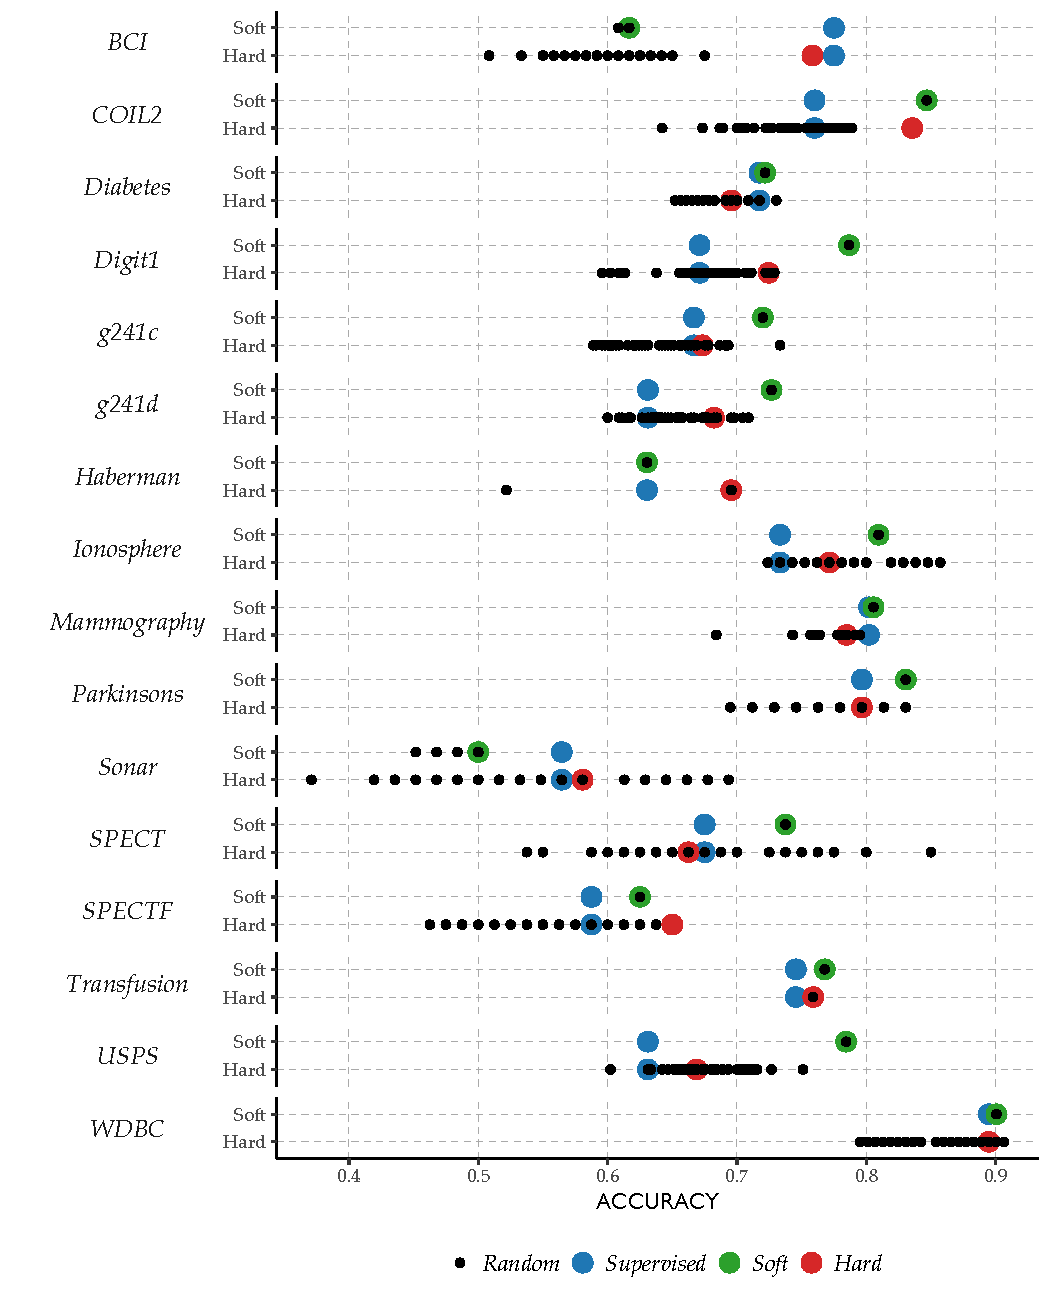
\includegraphics[width=\maxwidth]{figure/localoptima-1} \caption[Each black dot represents the performance of a randomly initialized run of the algorithm]{Each black dot represents the performance of a randomly initialized run of the algorithm. The red points indicate the performance of the hard-label procedure, initialized in the supervised solution. The green points indicate the performance of the soft-label procedure, initialized in the supervised solution. Blue points indicate the performance of the supervised solution. Notice the difference in the number of unique minima of the two procedures.}\label{fig:localoptima}
\end{figure}


\end{knitrout}


\subsection{Increasing the Number of Unlabeled Examples}
We study the effects of using an increasing number of unlabeled examples, while keeping the number of labeled examples fixed. The procedure is set us as follows: for each dataset we sample $L$ objects without replacement to form the labeled set. We choose $L>d$, the number of features in the dataset to ensure the supervised least squares solution is well-defined. We then sample an increasing number of unlabeled examples ($U=1,2,4,\dots,256$) without replacement, and use the remaining samples as the test set. Each classifier is trained on the labeled and unlabeled examples and their classification performance is evaluated on the test set. This procedure is repeated $1000$ times. Apart from the soft- and hard-label self-learning procedures, we also consider an \emph{Oracle} least squares solution, which has access to the labels of the unlabeled objects. This can be considered an upper bound on the performance of any semi-supervised learning procedure. The results are shown in Figure~\ref{fig:learningcurves}.

\begin{knitrout}
\definecolor{shadecolor}{rgb}{1, 1, 1}\color{fgcolor}\begin{figure*}
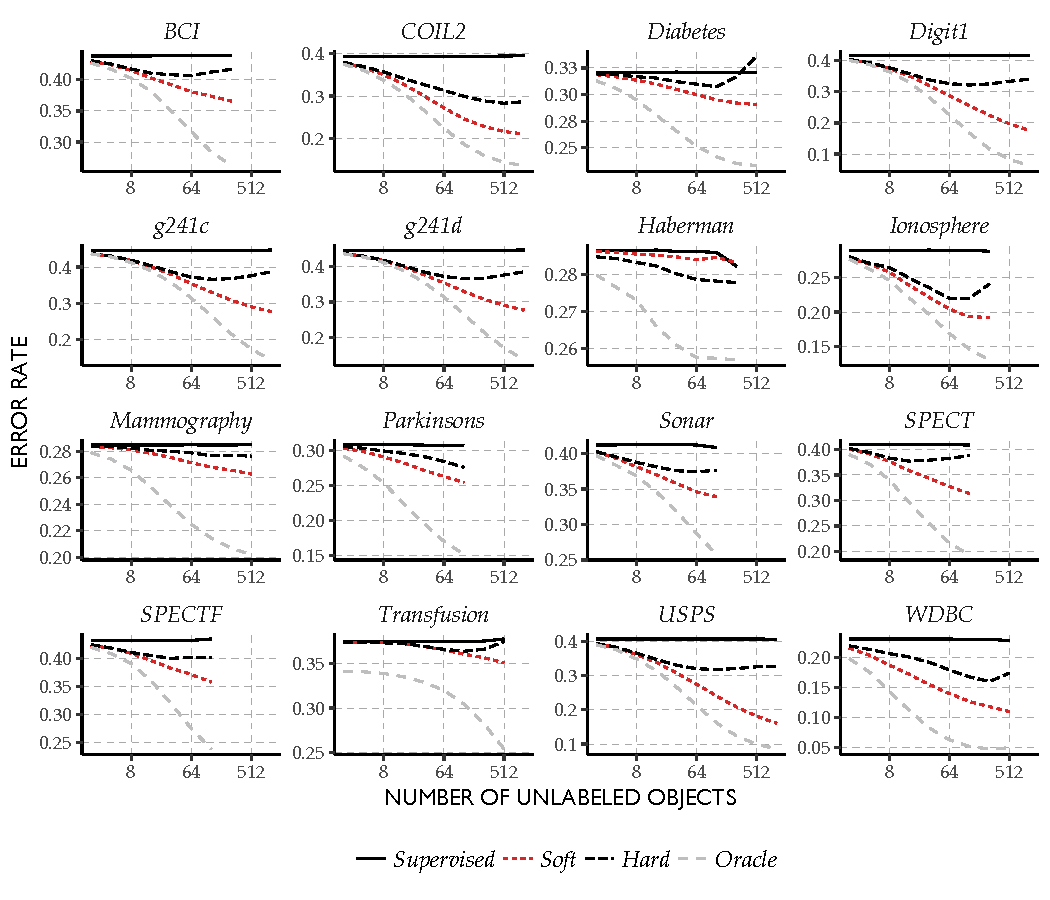
\includegraphics[width=\maxwidth]{figure/learningcurves-1} \caption[Classification errors for increasing amounts of unlabeled data]{Classification errors for increasing amounts of unlabeled data. The number of labeled objects remains fixed at a number larger than the dimensionality of the dataset to ensure the supervised solution is well-defined. Results are averaged over 1000 repeats.}\label{fig:learningcurves}
\end{figure*}


\end{knitrout}
The soft-label self-learning approach generally outperforms the hard-label approach when we increase the amount of unlabeled data. On this collection of datasets, the hard-label variant only outperforms the soft-label variant on the Haberman dataset. Moreover, for the hard-label variant performance can sometimes decrease as more unlabeled data is added. A partial explanation of the better behaviour of the soft-label variant can be found in the results from Figure~\ref{fig:localoptima}. These results suggest that while the hard-label objective has good local minima, there are many more local minima than in the soft-label case, making it less likely to reach a good one when starting from the supervised solution.

\section{Conclusion}
We studied a simple, straightforward semi-supervised least squares classifier that is related to an iterative method that dates back at least 60 years. We described it both in its historical context and by formulating it as a block coordinate descent procedure applied to a particular objective function. The resulting procedure can be considered a soft-label variant of self-learning and is an optimistic type of semi-supervised learning, as a contrast to pessimistic approaches to safe semi-supervised learning. We empirically showed that this simple procedure works well as an alternative to the more fickle hard-label self-learning. Generally, both procedures outperform the supervised solution.

\chapter[The Peaking Phenomenon in Semi-supervised Learning]{The Peaking Phenomenon\\in Semi-supervised Learning}
\chaptermark{Peaking in SSL}
\label{chapter:peaking}
\blfootnote{This chapter appeared as: Krijthe, J. H., \& Loog, M. 2016. The Peaking Phenomenon in Semi-supervised Learning. In A. Robles-Kelly, M. Loog, B. Biggio, F. Escolano, \& R. Wilson (Eds.), Structural, Syntactic, and Statistical Pattern Recognition. S+SSPR 2016. Lecture Notes in Computer Science, vol 10029. (pp. 299–309). Springer}


\begin{abstract}
For the supervised least squares classifier, when the number of training objects is smaller than the dimensionality of the data, adding more data to the training set may first increase the error rate before decreasing it.  This, possibly counterintuitive, phenomenon is known as peaking. In this work, we observe that a similar but more pronounced version of this phenomenon also occurs in the semi-supervised setting, where instead of labeled objects, unlabeled objects are added to the training set. We explain why the learning curve has a more steep incline and a more gradual decline in this setting through simulation studies and by applying an approximation of the learning curve based on the work by Raudys \& Duin.
\end{abstract}

\section{Introduction}
In general, for most classifiers, classification performance is expected to improve as more labeled training examples become available. The dipping phenomenon is one exception to this rule, showing for specific combinations of datasets and classifiers that error rates can actually increase with increasing numbers of labeled data \cite{Loog2012}.  For the least squares classifier and some other classifiers, the \emph{peaking phenomenon} is another known exception. In this setting, the classification error may first increase, after which the error rate starts to decrease again as we add more labeled training examples. The term peaking comes from the form of the learning curve: an example of which is displayed in \cref{fig:peaking}. 

\begin{knitrout}
\definecolor{shadecolor}{rgb}{1, 1, 1}\color{fgcolor}\begin{figure}
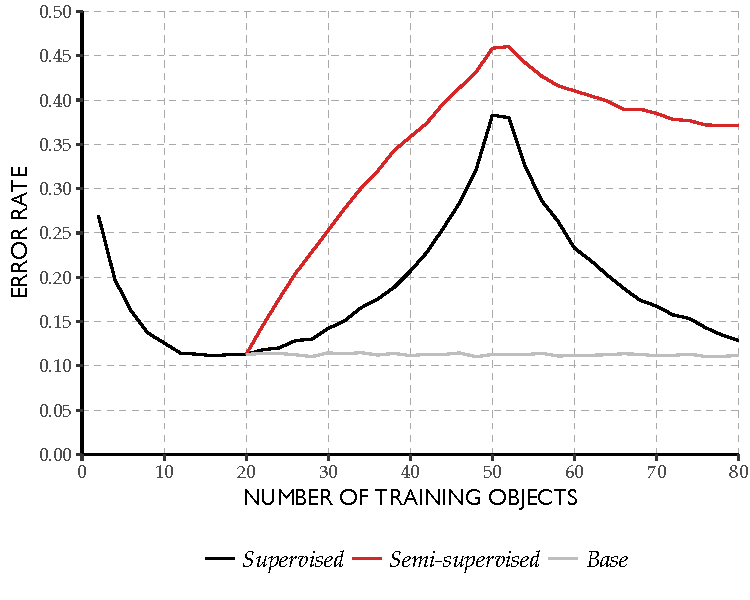
\includegraphics[width=\maxwidth]{figure/peaking-1} \caption{Empirical learning curves for the supervised least squares classifier (Eq.~\eqref{eq:solutionsupervised}) where labeled data is added and the semi-supervised least squares classifier (Eq.~\eqref{eq:solutionsemisupervised}) which uses 10 labeled objects per class and the remaining objects as unlabeled objects. ``Base'' corresponds to the performance of the classifier that uses the first 10 labeled objects for each class, without using any additional objects. Data are generated from two Gaussians in 50 dimensions, with identity covariance matrices and a distance of 4 between the class means.}\label{fig:peaking}
\end{figure}


\end{knitrout}

The term `peaking' is inspired by a different peaking phenomenon described by \citet{Hughes1968} (see also \citet{Jain1982}), who studies the phenomenon that the performance of many classifiers peaks for a certain number of features and then decreases as more features are added. In this work we consider a different peaking phenomenon that occurs when the number of training objects is increased, and the peak does not refer to a peak in performance, but a peak in terms of the classification error, after which performance starts increasing again. While this type of peaking also shows up in feature curves, where we increase the number of features, we focus on learning curves in terms of the number of training objects because it relates more closely to the question whether unlabeled data should be used at all in the semi-supervised setting.

The peaking phenomenon considered here is observed in \cite{Duin1995,Skurichina1996,Opper1995,Duin2000,Opper2001} for various classifiers in the supervised learning setting and \cite{Duin1995,Skurichina1999,Duin2000,Opper2001} additionally describe different ways to get rid of this unwanted behaviour, notably, by only considering a subset of relevant objects, by adding regularization to the parameter estimation, adding noise to objects, doing feature selection, or by injecting random features. 

\citet{Grunwald2014} describe a remarkably similar phenomenon in the context of fitting Bayesian linear regression models. They show that, in a setting similar to the one considered here, where the dimensionality of the model is fixed, too little regularization leads to a peaking phenomenon, as in the unregularized regression models considered in this chapter. They also construct an example where, when the number of variables used is inferred by the model as well, a peaking phenomenon continues to exist when the model is misspecified, while the Bayesian model does not exhibit a peak when the model is correctly specified. Their example also shows that for very high-dimensional models, the misspecified model is not guaranteed to converge to the best predictive model in the hypothesis space in terms of squared loss. Interestingly, considering our discussion on surrogate losses in previous chapters, the misspecified model does lead to good predictions in terms of the log-loss. They explain, using an information theoretic argument, for what types of misspecification this peaking behaviour occurs. 

While this peaking phenomenon has been observed for the least squares classifier when the amount of labeled data is increased, we find similar but worse behaviour in the semi-supervised setting.  Following the work in \citet{Duin1995} and \citet{Fan2008}, we study a particular semi-supervised adaptation of the least squares classifier in greater depth. An example of the actual behaviour is shown in \cref{fig:peaking}. When the amount of labeled objects remains fixed ($20$ in the figure) while we increase the amount of unlabeled data used by this semi-supervised learner, the peaking phenomenon changes in two ways: the error increases more rapidly when unlabeled data is added than when labeled data is added and after the peak the error decreases more slowly than when labeled data is added. The goal of this work is to describe and explain these effects. More specifically, we attempt to answer two questions:
\begin{enumerate}
\item What causes the performance in the semi-supervised setting to deteriorate faster than in the supervised case?
\item If we increase the amount of unlabeled data, will the performance of the semi-supervised learner converge to an error rate below the error rate of the supervised learner that does not take the additional unlabeled data into account?
\end{enumerate}
To answer these questions, we first revisit the supervised peaking phenomenon and explain its causes in \cref{section:supervisedpeaking}. In \cref{section:semi-supervised} we show how the results from \cref{section:supervisedpeaking} relate to the least squares classifier and how we specifically adapt this classifier to the semi-supervised setting. In \cref{section:incline,section:decline} we attempt to answer our two questions in two ways: firstly by adapting the learning curve approximation of \citet{Raudys1998} and secondly through simulation studies. We end with an investigation of the semi-supervised peaking phenomenon on some benchmark datasets.

\section{Supervised Peaking} \label{section:supervisedpeaking}
\citet{Raudys1998} attempt to explain the peaking phenomenon in the supervised case by constructing an asymptotic approximation of the learning curve and decomposing this approximation into several terms that explain the effect of adding labeled data on the learning curve. The classifier they consider is the Fisher linear discriminant, whose normal to the decision boundary is defined as the direction that maximizes the between-class variance while minimizing the within-class variance:
\begin{equation} \label{eq:fisherobjective}
\argmax_{\vec{w}} \frac{(\vec{w}^\top \vec{m}_1 - \vec{w}^\top \vec{m}_2)^2}{\vec{w}^\top W \vec{w}} \, ,
\end{equation}
where $\vec{m}_c$ is the sample mean of class $c$ and $W=\tfrac{1}{n} \sum_{c=1}^2 \sum_{i=1}^{N_c} (\vec{x}_{ci} - \vec{m}_c)(\vec{x}_{ci} - \vec{m}_c)^\top$ is the sample within-class scatter matrix. The solution is given by
\begin{equation} \label{eq:Wformulation}
\vec{w} = W^{-1} (\vec{m}_1-\vec{m}_2) \, .
\end{equation}
The intercept (or threshold value) that we consider in actual classification is right in between the two class means:
$-\frac{1}{2}(\vec{m}_1+\vec{m}_2)^\top \vec{w}$.  The peaking phenomenon occurs when $n=2N<p$, where $N$ is the number of (labeled) objects per class and $p$ is the dimensionality of the data. In this case, a pseudo-inverse needs to be applied instead of the regular inverse of $W$. This is equivalent to removing directions with an eigenvalue of $0$ and training the classifier in a lower dimensional subspace, a subspace whose dimensionality increases as more training data is added.

The goal of the analysis in \cite{Raudys1998} is to construct an approximation of the learning curve, which decomposes the error into different parts. These parts relate the observed peaking behaviour to different individual effects of increasing the number of training objects. To do this they construct an asymptotic approximation where both the dimensionality and the number of objects grows to infinity. An important assumption in the derivation, and the setting we also consider in our analysis, is that the data are generated from two Gaussian distributions corresponding to two classes, with true variance $\mathbf{I}$ and a Euclidean distance between the true means $\boldsymbol{\mu}_1$ and $\boldsymbol{\mu}_2$ of $\delta$. Lastly, objects are sampled in equal amounts from both classes.

The approximation of the learning curve is then given by\footnote{While going through the derivation we found a different solution than the one reported by \citet{Raudys1998}, which renders the last term in the formulation independent of $N$. This slightly changes the expressions in the explanation of the peaking behaviour.}
% $$
% R(N,p,\delta_d,\gamma,\mu_4) = \Phi \left\{ - \frac{\delta}{2} \sqrt{(1+\gamma^2)(1+ \frac{1}{N} (1+\frac{2 p}{\delta_d^2})+\frac{p}{\delta^2_d N^2})+\gamma^2 \frac{\mu_4}{4 \delta_d^2}}^{-1}\right\} \,.
% $$
% When we substitute estimates of $\delta_d^2$ and $\mu_4$ into this formulation
$$e(N,p,\delta) = \Phi \left\{ - \frac{\delta}{2} T_r \sqrt{(1+\gamma^2)T_\mu+\gamma^2 \frac{3 \delta^2}{4 p}}^{-1}\right\} \,,$$
where $\Phi$ is the cumulative distribution function of a standard normal distribution and $N$ is the number of objects per class.  The main quantities introduced are $T_\mu$, $T_r$, and $\gamma$ and \citet{Raudys1998} note that the approximation of the learning curve can be broken down to depend on exactly these three quantities all with their own specific interpretation:
%$$T_\mu=1+\frac{1}{N} + \frac{4 p^2}{\delta^2 N^2} + \frac{2 p^2}{\delta^3 N^3}$$
%which relates to how well we can estimate the means of the classes, $T_r=\sqrt{\frac{N}{2 p}}$ which relates to the reduction in features brought about by using  the pseudo-inverse and two terms relating to the estimation of the eigenvalues, $\gamma=\frac{\sqrt{V_d}}{E_d}$ and $T_{\textrm{eig}}=\frac{3 \delta^2 N}{8 p^2}$.
$$T_\mu=1+ \frac{1}{N} + \frac{2 p^2}{\delta^2 (2N-2) N}+\frac{p^2}{\delta^2 (2N-2) N^2}\,,$$
relates to how well we can estimate the means, $T_r=\sqrt{\frac{2 N-2}{p}}$ relates to the reduction in features brought about by using the pseudo-inverse and $\gamma$ is a term related to the estimation of the eigenvalues or $W$.  The $T_\mu$ and $T_r$ terms lead to a decrease in the error rate as $N$, the number of objects per class increases. This is caused by the improved estimates of the means and the increasing dimensionality. The $\gamma$ term increases the generalization error as $N$ increases, which is caused by the fact that the smallest eigenvalues are difficult to accurately estimate but can have a large effect on the computation of the pseudo-inverse.

When $n>p$ the pseudo-inverse is no longer necessary and other approximations of the learning curve can be applied. The comparison of these approximations in \cite{Wyman1990} shows that the approximation
$$
e(N,p,\delta) = \Phi \left\{ - \frac{\delta}{2}  \sqrt{T_\mu T_\Sigma}^{-1}\right\} \,,
$$
with $T_\mu=1+\frac{2 p}{\delta^2 N}$ and $T_\Sigma=1+\frac{p}{2 N - p}$ works reasonably well. The former term again relates to the estimation of the means while the latter term relates to the estimation of the within scatter matrix $W$.  \cref{fig:peaking-asymptotic-a} shows these approximations and the empirical learning curve on a simple dataset with 2 Gaussian classes, with a distance between the means of $\delta=4.65$.


\begin{knitrout}
\definecolor{shadecolor}{rgb}{1, 1, 1}\color{fgcolor}\begin{figure}
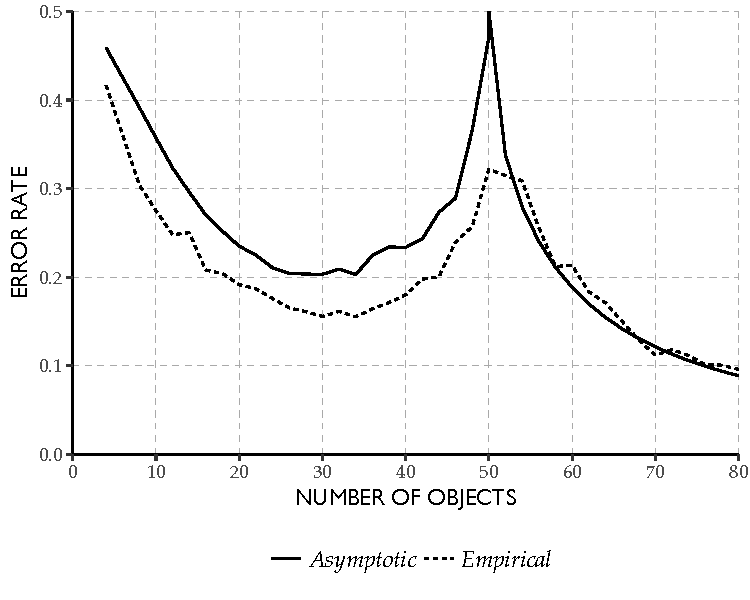
\includegraphics[width=\maxwidth]{figure/peaking-asymptotic-a-1} \caption{Empirical learning curves and their asymptotic approximations for different classifiers: Supervised learning curve corresponding to the formulation in Eq.~\eqref{eq:Wformulation}.}\label{fig:peaking-asymptotic-a}
\end{figure}


\end{knitrout}


\begin{knitrout}
\definecolor{shadecolor}{rgb}{1, 1, 1}\color{fgcolor}\begin{figure}
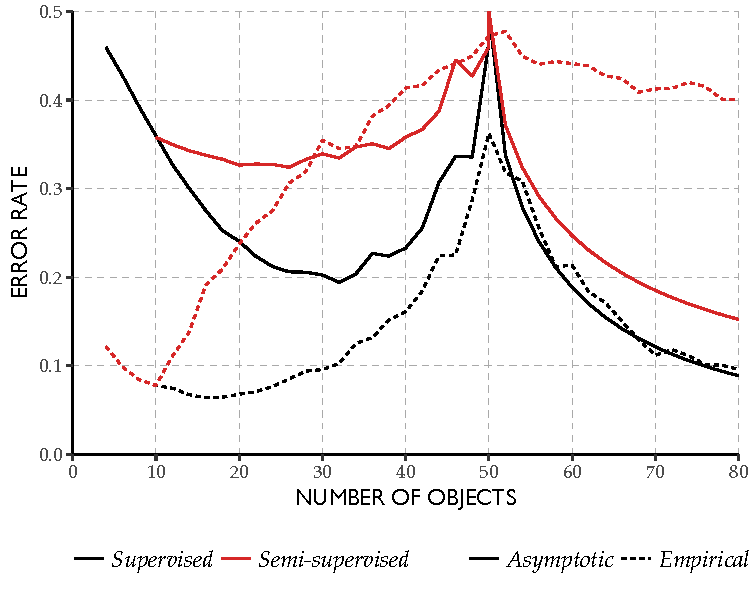
\includegraphics[width=\maxwidth]{figure/peaking-asymptotic-b-1} \caption{Empirical learning curves and their asymptotic approximations for different classifiers: Supervised and semi-supervised learning curves corresponding to the formulations in Eqs.~\eqref{eq:Tformulation}, \eqref{eq:solutionsupervised} and \eqref{eq:solutionsemisupervised}. Semi-supervised uses 5 labeled objects per class and the rest as unlabeled objects.}\label{fig:peaking-asymptotic-b}
\end{figure}


\end{knitrout}

\section{Semi-supervised Classifier} \label{section:semi-supervised}
Unfortunately for our analysis, the classifier studied by Raudys \& Duin does not correspond directly to the least squares classifier we wish to study, nor is it directly clear how their classifier can be extended to the semi-supervised setting.
% \cite{Fan2008} propose a slightly different formulation of the objective function that does allow for the incorporation of unlabeled data and which corresponds to the least squares classifier. It is based on the observation that the total scatter matrix, $T=\tfrac{1}{n}\sum_{i=1}^n (\vec{x}_i - \vec{m})(\vec{x}_i - \vec{m})^\top$, with $\vec{m}$ the overall mean of the data, can be decomposed as $T=B+W$. $B=\tfrac{1}{2}\sum_{c=1}^2 (\vec{m}_c - \vec{m})(\vec{m}_c - \vec{m})^\top$ is the between class scatter matrix. Because of this equality maximizing
% $$\frac{\vec{w}^\top T \vec{w} }{\vec{w}^\top W \vec{w} }$$
% has the same maximum as the objective in Equation \eqref{eq:fisherobjective} and we can write the solution as:
We therefore consider a slightly different version in which we follow \citet{Duin1995} and \citet{Fan2008}:
\begin{equation}
\vec{w} = T^{-1} (\vec{m}_1-\vec{m}_2) \label{eq:Tformulation} \, .
\end{equation}
Here $T$ is the total scatter matrix. This leads to the same classifier as Equation \eqref{eq:Wformulation} when $n>p$ \cite{Duin1995}. Moreover, when the data are centered ($\vec{m}=\vec{0}$) and the class priors are exactly equal it is equivalent to the solution of the least squares classifier, which minimizes the squared loss $(\vec{x}_i^\top \vec{w} - y_i)^2$ and whose solution is given by
\begin{equation}
\vec{w} = (\mathbf{X}^\top \mathbf{X})^{-1} \mathbf{X}^\top \vec{y} \, , \label{eq:solutionsupervised}
\end{equation}
where $\vec{y}$ is a vector containing a numerical encoding of the labels and $\mathbf{X}$ is the $L \times p$ design matrix containing the $L$ labeled feature vectors $\vec{x}_i$.

While Eq.~\eqref{eq:Tformulation} is equivalent to Eq.~\eqref{eq:Wformulation} when $n>p$, this solution is not necessarily the same in the scenario where $n<p$ (compare the dashed black lines in \cref{fig:peaking-asymptotic-a} and \cref{fig:peaking-asymptotic-b}). This makes it impossible to apply the results from \cite{Raudys1998} directly to get a quantitatively good estimator for the learning curve. Moreover, their proof is not easily adapted to this new classifier. This is caused by dependencies that are introduced between the total scatter matrix $T$ (which is proportional to $\mathbf{X}^\top \mathbf{X}$ in case $\vec{m}=\vec{0}$) and the mean vectors $\vec{m}_c$ that complicate the derivation of the approximation. Their result does, however, offer a qualitative explanation of the peaking phenomenon in the semi-supervised setting---as we will see in \cref{section:inclineasymptotic}.

How then do we adapt the least squares classifier to the semi-supervised setting? \citet{Fan2008} proposes to update $T$, which does not depend on the class labels, based on the additional unlabeled data. Equivalently, in the least squares setting, \citet{Shaffer1991} studies the improvement in the least squares classifier by plugging in a better estimator of the covariance term, $\mathbf{X}^\top \mathbf{X}$, which is equivalent to the update proposed by \citet{Fan2008}. We define our semi-supervised least squares classifier as this update:
\begin{equation}
\vec{w} = (\tfrac{L}{L+U} \mathbf{X}_\textrm{e}^\top \mathbf{X}_\textrm{e})^{-1} \mathbf{X}^\top \vec{y} \,. \label{eq:solutionsemisupervised}
\end{equation}
This is the semi-supervised learner depicted in \cref{fig:peaking}. Here $L$ is the number of labeled objects, $U$, the number of unlabeled objects and $\mathbf{X}_\textrm{e}$ the $(L+U) \times p$ design matrix containing all the feature vectors. The weighting $\tfrac{L}{L+U}$ is necessary because $\mathbf{X}_\textrm{e}^\top \mathbf{X}_\textrm{e}$ is essentially a sum over more objects than $\mathbf{X}^\top \vec{y}$, which we have to correct for.

\section{Why Peaking is More Extreme Under Semi-supervision} \label{section:incline}
One apparent feature of the semi-supervised peaking phenomenon is that before the peak occurs, the learning curve rises more steeply when unlabeled data are added vs. when labeled data are.

\subsection{Asymptotic Approximation} \label{section:inclineasymptotic}
To explain this behaviour using the learning curve approximation, we hold the term that relates to the increased accuracy of the estimate of the means, $T_\mu$, constant and consider the change in the approximation. As we noted before, the learning curve approximation is for a slightly different classifier, yet it might offer a qualitative insight as to the effect of only adding unlabeled data. Looking at the resulting curve in \cref{fig:peaking-asymptotic-b}, we indeed see that the semi-supervised approximation rises more quickly than the supervised approximation due to the lack of labeled data to improve the estimates of the mean. After the peak we see that the curve drops off less quickly for the same reason. The approximation, however, is not a very accurate reflection of the empirical learning curve.

\subsection{Simulation of Contributions}
\begin{knitrout}
\definecolor{shadecolor}{rgb}{1, 1, 1}\color{fgcolor}\begin{figure}
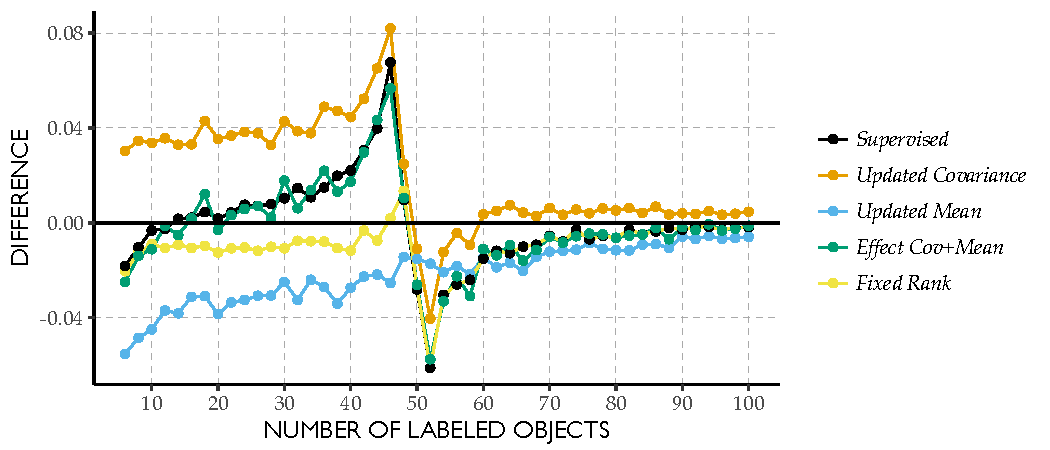
\includegraphics[width=\maxwidth]{figure/contributions-1} \caption[Average gain in error rate by adding $2$ additional objects to the training set, either in a supervised way, by adding labeled objects, or by only using them to improve the estimator of the total scatter (covariance)]{Average gain in error rate by adding $2$ additional objects to the training set, either in a supervised way, by adding labeled objects, or by only using them to improve the estimator of the total scatter (covariance).}\label{fig:contributions}
\end{figure}


\end{knitrout}
Because the approximation used does not approximate the empirical learning curve very well, the question remains whether the lack of the updating of the means based on new data fully explains the increase in the semi-supervised learning curve over the supervised learning curve. To explore this, we decompose the change in the supervised learning curve into separate components by calculating the change in the error rate from adding data to improve respectively the estimator of the total covariance, $T$, the means or both at the same time. The result is shown in \cref{fig:contributions}.

To do this we compare the difference in error of the semi-supervised classifier that has two additional unlabeled objects available to the supervised classifier that does not have these unlabeled data available. We see that adding these objects typically increases the error rate when $n<p$.  We then compare the error of the supervised classifier to the one where we remove $2$ labels and the classifier where we do not remove these labels. By negating this difference we get the value of having two additional labels. We see that for this dataset this effect always decreases the error.  Adding up the effect of adding unlabeled objects to the effect of having additional labels, we find this approximates the total effect of adding labeled objects very well. It seems, therefore, that in the semi-supervised setting, by not having additional labels, the positive effect of these labels as shown \cref{fig:contributions} is removed, explaining the difference between the supervised and semi-supervised setting.

It is also clear from these results that peaking is caused by the estimation of the inverse of the covariance matrix, which leads to an increase in the error before $n>p$. To understand why this happens, consider the ``Fixed rank'' curve in \cref{fig:contributions}. This curve shows the change in terms of the error rate when we add two labeled objects but leave the rank of the covariance matrix unchanged during the calculation of the inverse, merely considering the largest $n$ eigenvectors of the newly obtained covariance matrix that was estimated using $n+2$ objects. Since this tends to decrease the error rate, the error increase for the other curve may indeed stem from the actual growth of the rank. Especially when $n$ is close to $p$, the eigenvalues of the dimensions that are added by increasing the rank become increasingly hard to estimate. This is similar to the $\gamma$ term in the approximation, which captures the difficulty of estimating the eigenvalues for these directions.

\begin{knitrout}
\definecolor{shadecolor}{rgb}{1, 1, 1}\color{fgcolor}\begin{figure}
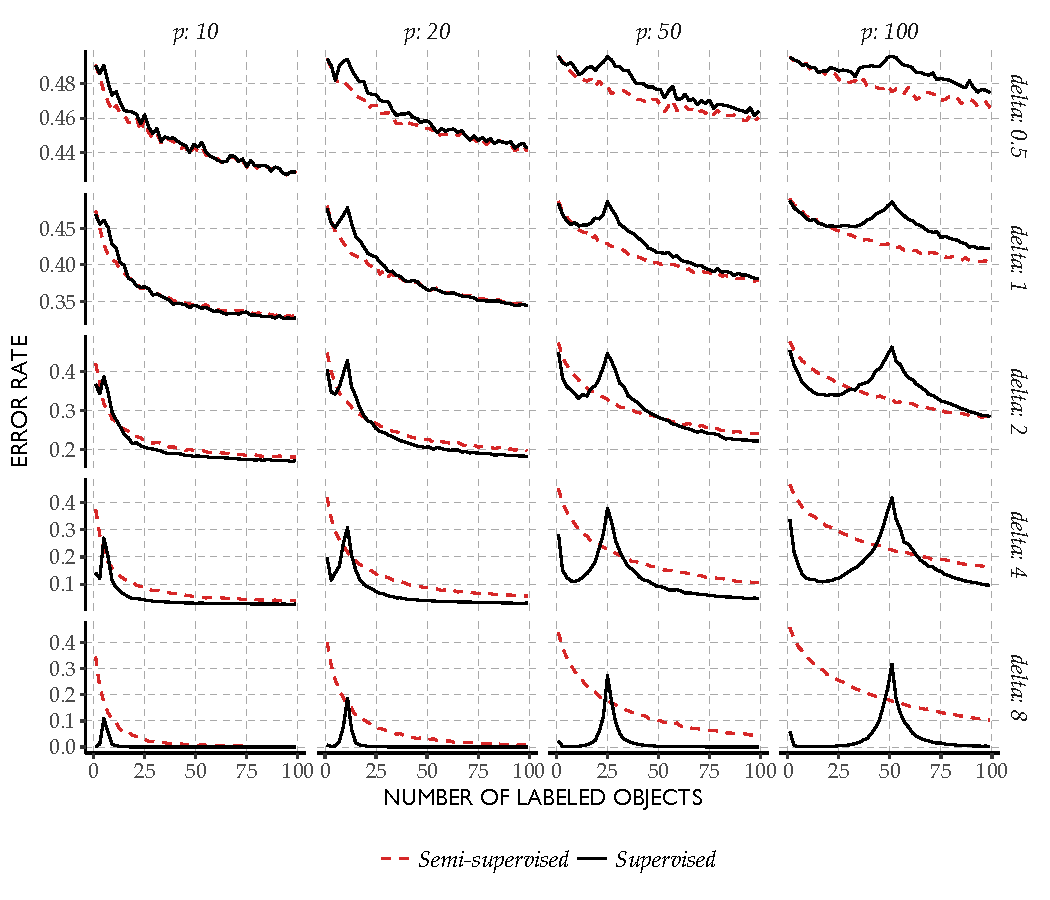
\includegraphics[width=\maxwidth]{figure/infinitedata-1} \caption[Learning curves for the supervised learner and the semi-supervised learner with infinite amounts of unlabeled data for different dimensionalities, $p$, and distances between the means, $\delta$]{Learning curves for the supervised learner and the semi-supervised learner with infinite amounts of unlabeled data for different dimensionalities, $p$, and distances between the means, $\delta$.}\label{fig:infinitedata}
\end{figure}


\end{knitrout}

\section{Convergence to a Better Solution than the Base Learner?} \label{section:decline}

The slow decline of the error rate after the peak in the learning curve begs the question whether the semi-supervised learner's error will ever drop below the error of the original supervised learner. If not, it would be worthwhile to refrain from using the semi-supervised learner in these settings.  The approximation in \cref{fig:peaking-asymptotic-b} indicates that the learning curve will decline more slowly when $n>p$ when unlabeled data are added. From this approximation, however, it is not clear if and under which circumstances the error of the semi-supervised classifier will improve over the base learner if larger amounts of unlabeled data become available.

To investigate this issue we consider, for the two-class Gaussian problem with different dimensionalities, $p$, and different distances between the means, $\delta$, whether adding infinite unlabeled data improves over the supervised learner, for different amounts of limited labeled data. We can simulate this by setting the true means as $\boldsymbol{\mu}_1=-\tfrac{\delta}{2 \sqrt{p}}\vec{1}$ and $\boldsymbol{\mu}_2=+\tfrac{\delta}{2 \sqrt{p}}\vec{1}$. In this case, when the amount of unlabeled data increases, the total scatter matrix will converge to
$$
T = \vec{I} + \vec{1} \vec{1}^\top \frac{1}{4} \frac{\delta^2}{p} \,.
$$
Using this we can calculate the semi-supervised classifier based on an infinite unlabeled sample and with a finite amount of labeled data. The results are shown in \cref{fig:infinitedata}.

We observe that the dimensionality of the data does not have a large effect on whether the semi-supervised learner can outperform the supervised learner. It merely shifts the peak while qualitatively the differences between the supervised and semi-supervised curves remain the same. If we decrease the Bayes error by moving the means of the classes further apart, however, there are clear changes. For small distances between the means, the semi-supervised learner generally does increase performance for a larger range of sizes of the labeled set, while for larger distances this is no longer the case and the semi-supervised solution is typically worse than the supervised solution that does not take the unlabeled data into account.

\section{Observations on Benchmark Datasets}
The goal of this section is to observe the semi-supervised peaking phenomenon on several benchmark datasets (taken from \cite{Chapelle2006} and \cite{Lichman2013}) and relate these observations to the results in the previous sections. We generate semi-supervised learning curves for eight benchmark datasets as follows. We select $L=\lceil p/2 \rceil$ where $p$ is the dimensionality of the dataset after applying principal component analysis and retaining as many dimensions as required to retain $99\%$ of the variance. 

We then randomly, with replacement, draw additional training samples, with a maximum of $100$ for the smaller datasets and $1000$ for the larger datasets. We also sample a separate set of $1000$ objects with replacement to form the test set. The additional training samples are used as labeled examples by the supervised learner and as unlabeled samples for semi-supervised learning. We repeat this process $100$ times and average the results. These averaged learning curves are shown in \cref{fig:benchmark}.

\begin{knitrout}
\definecolor{shadecolor}{rgb}{1, 1, 1}\color{fgcolor}\begin{figure}
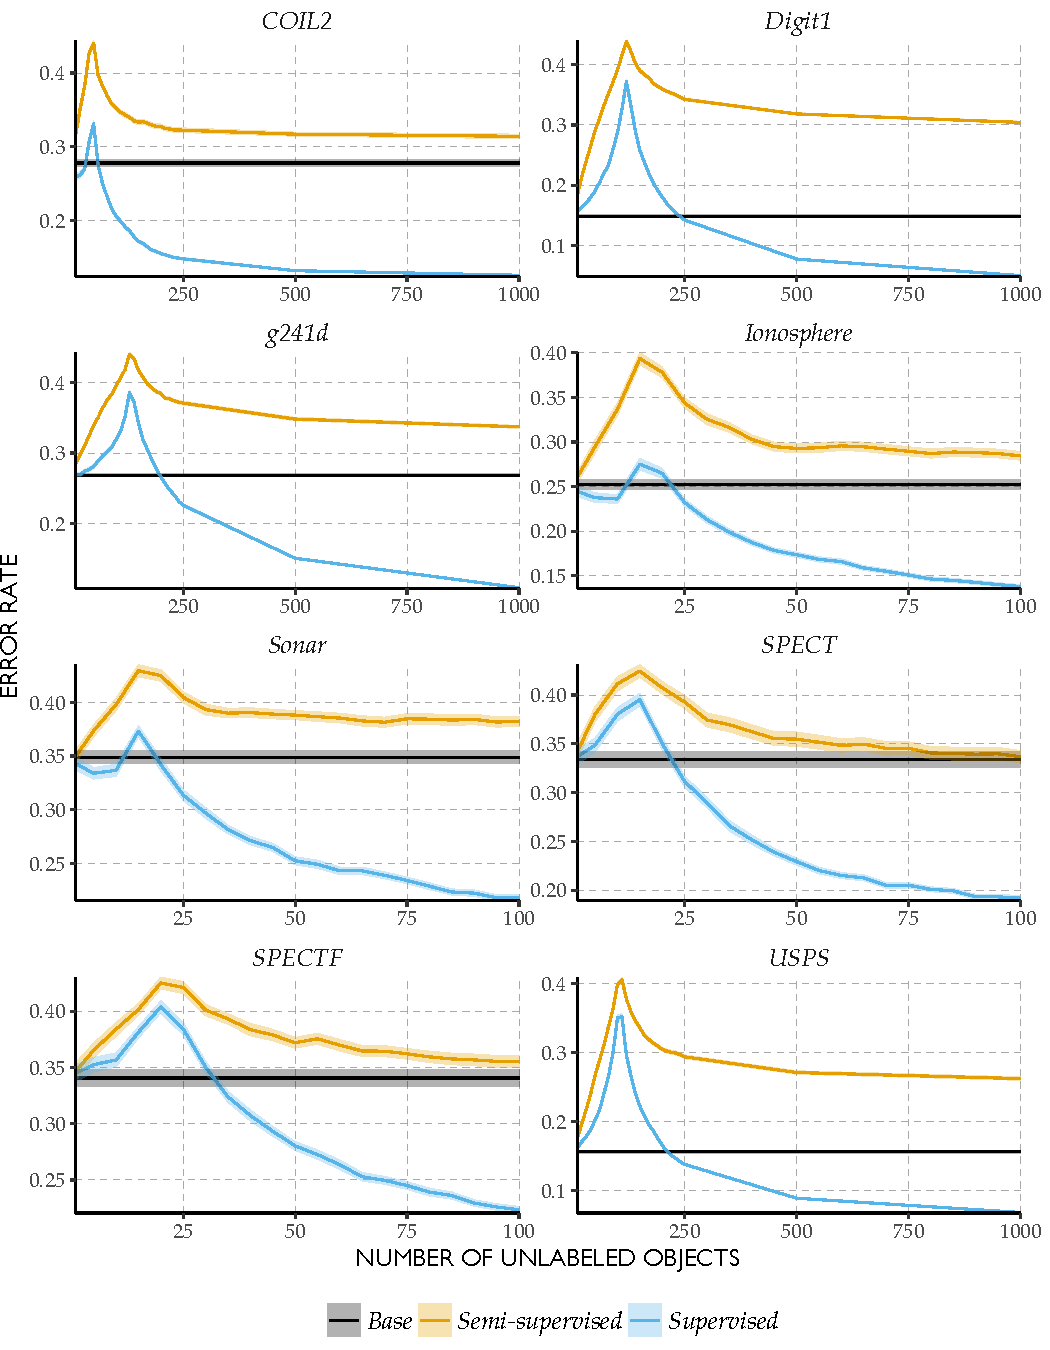
\includegraphics[width=\maxwidth]{figure/benchmark-1} \caption[Learning curves on benchmark datasets]{Learning curves on benchmark datasets. The number of labeled objects is equal to $\lceil p/2 \rceil$. For the semi-supervised curve we add more unlabeled data, for the supervised curve more labeled data. ``Base'' shows performance of the supervised classifier using only the original $\lceil p/2 \rceil$ objects. For each dataset 100 curves where generated and averaged. Shaded area (small) indicates the standard error around the mean.}\label{fig:benchmark}
\end{figure}


\end{knitrout}

Both behaviours studied in the previous sections, the steeper ascent in the semi-supervised setting before the peak and the slower decline after the peak, are apparent on these example datasets. We also notice that for most of these datasets it seems unlikely that the semi-supervised learning will improve over the base classifier. This may suggest we are in a scenario similar to the large difference between the means in \cref{fig:infinitedata}. The exception is the SPECT and SPECTF datasets, where the situation is more similar to the smaller $\delta$. Notice that for all datasets it is still possible we are in a situation similar to $\delta=2$ in \cref{fig:infinitedata}: while adding unlabeled data does not help with the given amount of labeled examples, this effect might reverse if a few more labeled objects become available.

\section{Discussion and Conclusion}
In this work, we have studied the behaviour of the learning curve for one particular semi-supervised adaptation of the least squares classifier. This adaptation, based on the ideas from \citet{Shaffer1991} and \citet{Fan2008}, was amenable to analysis. It is an open question what the typical learning curve for other semi-supervised least squares adaptations looks like, such as self-learning or the constraint based approach in \citet{Krijthe2015} where we first noticed this behaviour and which inspired us to look into this phenomenon. The lack of a closed form solution in these cases makes it more difficult to subject them to a similar analysis.  Nevertheless, the current study does provide insight in the additional problems that small samples entail in the semi-supervised setting and largely explains the learning curve behaviour, at least for the specific semi-supervised learner considered.
\cleartoverso
\null
\thispagestyle{empty}
\newpagecolor{ThesisGreen}\afterpage{\restorepagecolor}
\newpage
\renewcommand{\mypartpic}{cover/part3.pdf}
\AddToShipoutPicture{\PartPic}
\part{REPRODUCIBILITY}
\ClearShipoutPicture

\chapter[Reproducible Pattern Recognition Research]{Reproducible Pattern Recognition Research:\\The Case of Optimistic SSL}
\chaptermark{Reproducible Pattern Recognition Research}
\label{chapter:reproducing}
\blfootnote{This chapter appeared as: Krijthe, J. H., \& Loog, M. 2016. Reproducible Pattern Recognition Research: The Case of Optimistic SSL. In B. Kerautret, M. Colom, \& P. Monasse (Eds.), Reproducible Research in Pattern Recognition. RRPR 2016. Lecture Notes in Computer Science, vol 10214. (pp. 48–59). Springer}


\begin{abstract}
In this paper, we discuss the approaches we took and trade-offs involved in making a paper on a conceptual topic in pattern recognition research fully reproducible. We discuss our definition of reproducibility, the tools used, how the analysis was set up, show some examples of alternative analyses the code enables and discuss our views on reproducibility.
\end{abstract}

\section{Introduction}
The goal of this work is to describe and discuss the choices involved in making the results of a conceptual work in pattern recognition fully reproducible. Conceptual, here, refers to the type and goal of the analysis that was done in that work: using simulations and experiments, it tries to improve our understanding of one or more methods, rather than apply an existing method to some new application or introduce supposedly novel approaches. The work in question is our paper on \textit{Optimistic Semi-supervised Least Squares Classification} \citep{Krijthe2016a}, which reports on two ways in which a supervised least squares classifier can be adapted to the semi-supervised setting, the connections between these two approaches and why one of these approaches often outperforms the other.

The conceptual nature of the work has particular advantages in making it reproducible: the data required to run experiments can easily be made available or, for simulated datasets, data are not required and the code to run the experiments is relatively self-contained, i.e. it has few dependencies on code outside this project. One could argue that for these types of projects, there is no reason \emph{not} to make results reproducible. We notice, however, that in practice, trade-offs and problems still come up. We will discuss our experience in this paper and use it as a case study to discuss the uses of reproducibility in pattern recognition research.

We will start by giving a short summary of the original paper on optimistic semi-supervised learning. We will then discuss what we mean by reproducibility and discuss the tools and strategies used here. After some examples of alternative analyses enabled by the reproducible nature of the work, we end with a discussion on the relevance of reproducibility in pattern recognition research.

\section{Summary of Optimistic SSL}
In supervised classification, classifiers are trained using a dataset of input/output pairs $\{(\mathbf{x}_i,y_i)\}^L_{i=1}$, where $\mathbf{x}_i$ is a $d$-dimensional input vector and $y_i$ is a binary outcome encoded using some value $m$ for one class and $n$ for the other. In semi-supervised learning, one attempts to use an additional set of unlabeled data $\{(\mathbf{x}_j)\}^U_{j=1}$ to improve the construction of a classifier to solve the supervised learning task. Semi-supervised learning is an active area of research due to its promise of improving classifiers in tasks where labeling objects is relatively expensive, or unlabeled data is inexpensive to come by.

The goal of the work in \cite{Krijthe2016a} is to study two different ways to adapt the supervised least squares classifier to the semi-supervised learning setting. The supervised least squares classifier for the two-class problem is defined as the linear classifier that minimizes the quadratic loss on the labeled objects or, equivalently, least squares regression applied to a numeric encoding of the labels, with the following objective function:
\begin{equation}
J_s(\mathbf{w}) = \| \mathbf{X} \mathbf{w}-\mathbf{y} \|^2 + \lambda \|\mathbf{w} \|^2 \,, \nonumber
\end{equation}
where $\mathbf{X}$ is the $L \times d$ design matrix of the labeled objects, $\mathbf{w}$ refers to the weights of the linear classifier and $\lambda$ is a regularization parameter. We now define two straightforward ways to include the unlabeled data in this objective function. The first we refer to as the \emph{label based objective}, since it treats the missing labels of the unlabeled data as a vector $\mathbf{u}$ that we should minimize over:
$$
J_l(\mathbf{w},\mathbf{u}) = \| \Xe \mathbf{w}-\begin{bmatrix} \mathbf{y} \\ \mathbf{u} \end{bmatrix} \|^2 + \lambda \|\mathbf{w} \|^2 \,,
$$
where $\Xe$ is an $(L+U) \times d$ design matrix containing the $d$ feature values for all, labeled and unlabeled, objects.
A second way to include the data is to consider that each unlabeled object belongs to one of two classes, and we can assign each object a responsibility: a probability of belonging to each class. If the classes are encoded as $m$ and $n$, for instance $-1$ and $+1$, this \emph{responsibility based objective} is defined as:
\begin{align}
J_r(\mathbf{w},\mathbf{q}) = & \| \mathbf{X} \mathbf{w}-\mathbf{y} \|^2 + \lambda \|\mathbf{w} \|^2 \nonumber + \sum_{j=1}^{U}  q_j (\mathbf{x}_j^\top \mathbf{w} - m)^2  + (1-q_j) (\mathbf{x}_j^\top \mathbf{w} - n)^2 \,. \nonumber
\end{align}

The first result from the paper is that applying block coordinate descent to these objectives -- where we alternate between minimizing over $\mathbf{w}$ and $\mathbf{u}$ respectively $\mathbf{q}$ -- the second procedure turns out to be equivalent to the well-known \emph{hard-label self-learning} approach applied to the least squares classifier, while the first approach is equivalent to a \emph{soft-label self-learning}, similar to a method that was originally proposed for regression as early as the 1930s \cite{Healy1956}.

The second result from the paper \cite{Krijthe2016a} is that the soft-label variant typically outperforms the hard-label variant on a set of benchmark datasets. In the paper we showed these results in terms of the error rate on an unseen test set: the learning curves of the performance for different amounts of unlabeled data are typically lower for the soft-label variant than for the hard-label variant. We will revisit these results in \cref{section:exampleperformance}, by showing how to adapt the code to not only consider the performance in terms of the error rate, but in terms of the quadratic loss used by the classifier as well.

The third result is a study of one reason for the performance difference by looking at the effect of local minima on the optimization problems posed by both approaches. We find that the label based objective corresponding to the soft-label variant has much fewer local minima for the optimization to get stuck in, compared to the hard-label variant, which often gets stuck in a bad local minimum, even though a better local minimum may be available.

\section{Reproducibility}

\subsection{Definition of reproducibility}
Reproducibility and replicability of experiments has gained increasing interest both in science in general \citep{Goodman2016a} and in pattern recognition/computer vision/machine learning as well \citep{Drummond2009,Donoho2009}. Much of this interest can be attributed to what some call the ``Reproducibility crisis'' in science: many published results can not be replicated by others trying to verify these results. Perhaps the most visible and laudable effort to estimate the scale of this problem in one scientific discipline has been the Open Science Collaboration's efforts in Psychology \citep{OpenScienceCollaboration2015} which find that by some measures of replicability, the results of less than half of the $100$ studies selected for replication could actually be replicated. A related, but different phenomenon is the ``credibility crisis'' \citep{Donoho2009} which refers to the decrease in the believability in computational scientific results caused by the increasing difficulty to understand exactly how results were obtained based on the textual description alone.

While ``replicability is not reproducibility'' \citep{Drummond2009}, these terms on their own may already refer to different things. \citet{Goodman2016a} attempts to give clear definitions for different notions of reproducing a result. In this paper, we are mostly concerned with what they call \emph{methods reproducibility}, meaning the ability of different researchers to reproduce exactly the same figures and tables of results based on the data, code and other artefacts provided by the original authors. Like \citet{Patil2016}, we will refer to this simply as \emph{reproducibility}. Note that the moniker reproducibility does not say anything about the correctness of results, only that they can be obtained again by a different researcher.

Also like \citet{Patil2016}, we will use the word \emph{replicability} to what \citet{Goodman2016a} calls \emph{results reproducibility}: the ability to obtain the results that support the same conclusion by an independent study. Here independent study is still vaguely defined to mean that we set up a new study, where we gather and analyse data using a procedure that ``closely resembles'' the procedures used in the original work.  This is what the ``reproducibility crisis'' we mentioned at the start of this section refers to: not being able to obtain the same results by such studies. In the pattern recognition context, this definition could often come down to the exact same thing as reproducibility. The definition by \citet{Patil2016} is slightly more explicit and considers a study to be a replication if the population, question, hypothesis, experimental design and the analysis plan remain fixed, but the analyst and the code, for instance, have been changed. For a proper definition of a replication in pattern recognition research, one aspect of a replication could be a re-implementation of methods. We will come back to this in the discussion.

The reason we attempt to be so explicit about our definitions here is that the meaning of the words reproducibility and reproducibility is sometimes interchanged by other authors. Note, for instance, that by our definitions, the reproducibility crisis is best referred to as the replicability crisis. Or consider \citet{Drummond2009} who refers to methods reproducibility as replicability, and uses reproducibility to mean obtaining the same result using an independent study. 

While our definition of reproducibility only concerns the reproduction of the results in the original paper, we will illustrate that having reproducible results reduces the friction to make small changes to the code to explore alternative analyses. This allows one to explore, for instance, how sensitive the results are to particular parameter choices made be the original authors, or whether the method also works for slightly different datasets. In other words, like in a replication, where many things are changed at once to see whether a result can still be obtained, these small changes teach us something about the robustness of the results.

Even if we stick to our definition of `reproduce exactly the results', there are several levels at which this can be interpreted for a pattern recognition study like ours. We could, for instance, consider the following levels:
\begin{itemize}
\item Final paper can be reproduced from the source text
\item Figures and tables can be generated from results of computations
\item Results of computations can be generated from experiment datasets
\item Experiment datasets can be generated from raw data 
\end{itemize}
All using steps for which open source code is available. Although we consider a paper reproducible when all these steps are fulfilled, in practice we will show that for many of the benefits of reproducibility, it may be useful to consider these as separate steps: to explore the effect of a different outcome measure, we may not want to redo the computations. Or for a particular experiment, the preprocessing applied to the raw data may not be particularly relevant, as long as we have the processed data.

\subsection{Strategy for Reproducibility}
All the code used to produce the results in \citep{Krijthe2016a} is written in the R programming language \citep{RCoreTeam2016}, while the paper itself is a combination of Latex and R code to generate the figures. The two are combined using the knitr package \cite{Xie2014}. knitr allows one to intersperse Latex with blocks of R code that get executed and turned into Latex expressions or figures before the Latex document is compiled. This allows for the code that generates the figures to be placed where one would usually place a figure environment in the Latex document, so that everything that visually becomes part of the paper is defined in a single document. One of the advantages of this approach is that the author can be sure that the figures and tables in the paper were actually generated by this code, i.e. the code did not inadvertently change in the meantime.

In principle, one could also include the code for the experiments itself in this document. We noticed, however, that even for projects of this relatively small size, and even though knitr is able to optionally cache results, we found it more convenient to place the code of the experiments in separate files, save the results to an R data file, and then load these result files to be used in the generation of the figures in the knitr document.

The advantage of this particular approach to splitting the computations across files was that we could easily transfer the experiment code to a compute server to run the experiments, while writing the document. A disadvantage of not including the experiment code in the final document is that it increases the possibility that the chain of reproducibility is broken: for instance, we could apply some transformation to the data between the time the experiments where run and the figures are generated and forget, or accidentally save or load an old result file.

Another trade-off was between writing code for this particular analysis project or splitting code off into separate packages. For instance, for the implementations of the classifiers, we decided to make these part of a larger package of methods for semi-supervised learning \cite{Krijthe2016rssl}. This makes the methods and some code used to run experiments available for other applications. It also made sense here, since this project was part of a larger research programme into semi-supervised learning. The downside is that it introduces dependencies between projects. The main practical lesson we learned here is to save the reference to the particular version that was used to generate the results in the paper in the version control system, so that future changes do not effect one's ability to reproduce the results.

Similar to the implementations of the methods, we split the code used to load the datasets into a separate project, to be used for other projects. These scripts download the data and save them locally, unless this is already done previously.

\section{Examples}
\label{section:exampleperformance}
In this section we will show some additional analyses that are possible by changing the original code from \citet{Krijthe2016a} and that lead to some additional insights into the methods covered in the paper. The examples shown here are meant to illustrate that reproducible results have utility beyond the mere fact that we are sure how the results were produced: it allows for small changes by readers that can lead to additional insights. We order the examples by the size of the changes to the code required to obtain the results.

\subsection{Changing an Example Figure}
We start with the simplest case where small changes to the code that generates a figure can help illustrate a point. In the original paper we give an example why the soft-label self-learning variant would update the decision boundary using the unlabeled objects, and that this updating depends on the location of the unlabeled objects. Here we change the location of the unlabeled objects, by changing the line \inlinecode{X\_u <-  matrix(c(-1, 4), 2, 1)} to \inlinecode{X\_u <-  matrix(c(-1, 0.5), 2, 1) } to show that when the decision values for all unlabeled objects are within $[-1,1]$, the soft-label self-learning is no different than the supervised solution. The result is shown in \cref{fig:additional-simple-example}. Note that this would be a case where an interactive version of the plot could be illustrative, instead of manually changing values and regenerating the plot.

\begin{knitrout}
\definecolor{shadecolor}{rgb}{1, 1, 1}\color{fgcolor}\begin{figure}
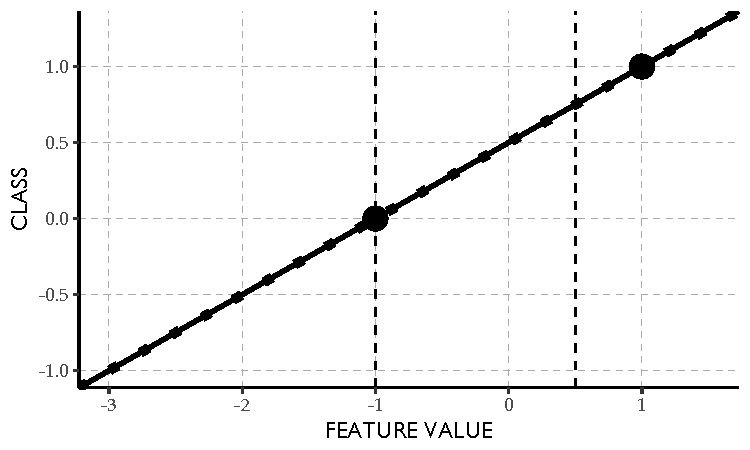
\includegraphics[width=\maxwidth]{figure/additional-simple-example-1} \caption[Example of the first step of soft-label self-learning]{Example of the first step of soft-label self-learning. The circles indicate two labeled objects, while the dashed vertical lines indicate the location of two unlabeled objects. The solid line is the supervised decision function. A dotted line indicates the updated decision function after finding the labels that minimize the loss of the supervised solution and using these labels as the labels for the unlabeled data in the next iteration. This last line is barely visible because the unlabeled data do not cause an update of the decision function in this case.}\label{fig:additional-simple-example}
\end{figure}


\end{knitrout}

\subsection{Changing the Outcome Quantity for the Learning Curves}
In the original paper, we report the error rate on a test set, for a fixed number of labeled training examples and an increasing amount of unlabeled examples. Alternatively, one might be interested in the performance in terms of the loss, instead of the classification error. Since this quantity was already computed during the experiment, we need not redo the experiment: a simple change in the code to plot the results suffices. More explicitly, we simply change the line \inlinecode{filter(Measure=="Error")} to \inlinecode{filter(Measure=="Average Loss Test")}.

\begin{knitrout}
\definecolor{shadecolor}{rgb}{1, 1, 1}\color{fgcolor}\begin{figure*}
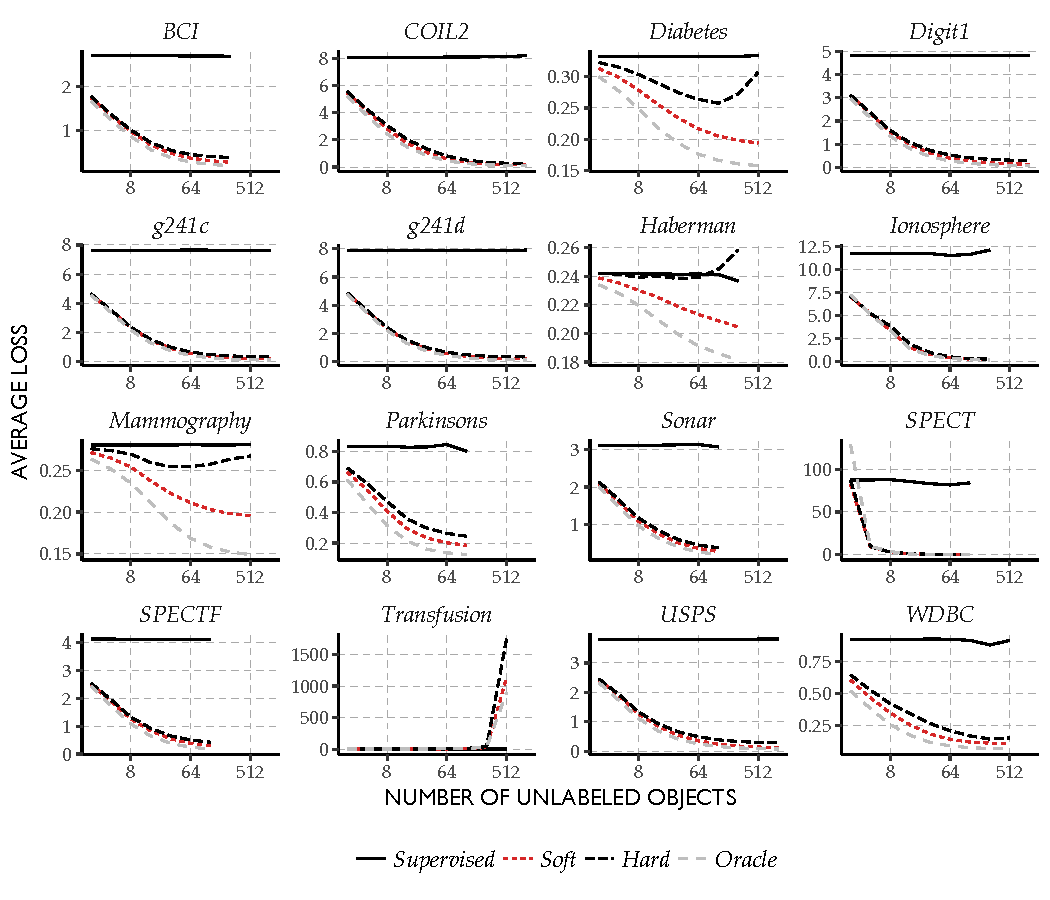
\includegraphics[width=\maxwidth]{figure/learningcurves-loss-1} \caption[Average squared loss on the test set for increasing amounts of unlabeled training data]{Average squared loss on the test set for increasing amounts of unlabeled training data. The number of labeled objects remains fixed at a number larger than the dimensionality of the dataset to ensure the supervised solution is well-defined. Results are averaged over 1000 repeats. Oracle refers to the supervised classifier that has access to the labels of all the objects.}\label{fig:learningcurves-loss}
\end{figure*}


\end{knitrout}

The results in \cref{fig:learningcurves-loss} show an interesting discrepancy when compared to the results in terms of the error rate: here in all cases the soft-label variant outperforms the hard-label variant, even on the dataset (Haberman) where it did not in terms of the error rate. Additionally, the loss starts increasing in more cases than for the error rate, especially for the hard-label variant.

\subsection{Sensitivity to Random Seed}
In the original work, we gave an example of a dataset where the hard-label self-learner is clearly outperformed by the soft-label self-learner. One might wonder how sensitive this dataset is to slight perturbations: is hard-label self-learning always much worse in this type of dataset or does it depend on the particular seed that was chosen when generating the data? This can be easily checked by changing the random seed and computing the classifiers. 

In \cref{fig:example-additional} we show two common configurations we find when we change the random seed. These configurations are qualitatively different from the result reported in the paper. In one case, there is no big difference between the two classifiers, unlike the result in the original work, while in the other, the hard-label self-learner gives deteriorated performance for a different reason: it assigns all objects to a single class. 

These results show that the original example is not stable to changes in the random seed. However, the conclusion that soft-label self-learning does not suffer from as severe a deterioration in performance as hard-label self-learning still holds. Our experience generating these additional examples does indicate, though, that other configurations than the prototypical example given in the paper are just as likely, if not more likely, to occur.

\begin{knitrout}
\definecolor{shadecolor}{rgb}{1, 1, 1}\color{fgcolor}\begin{figure}
\subfloat[Small difference\label{fig:example-additional1}]{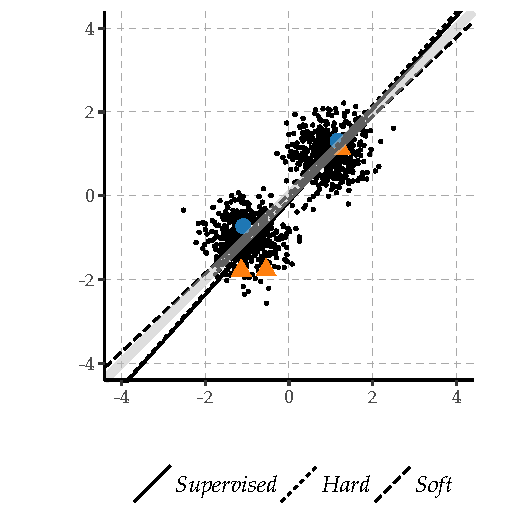
\includegraphics[width=.49\linewidth]{figure/example-additional-1} }
\subfloat[Hard-label single class\label{fig:example-additional2}]{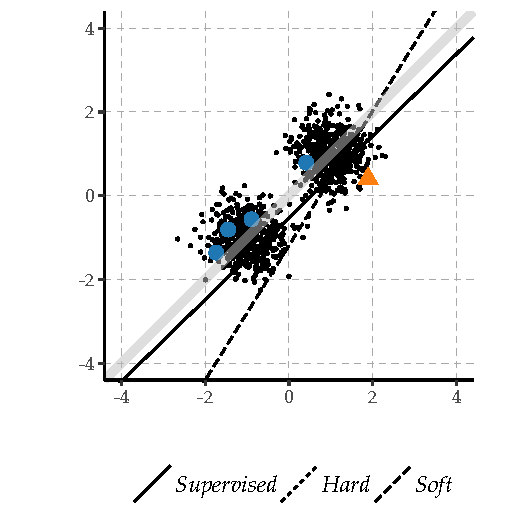
\includegraphics[width=.49\linewidth]{figure/example-additional-2} }\caption[Additional examples of the behaviour of hard-label and soft-label self-learning]{Additional examples of the behaviour of hard-label and soft-label self-learning. Light-grey line indicates true decision boundary. In (a), there is only a minor difference between soft-label and hard-label self-learning. In (b), the hard-label self-learner is not visible and assigns all objects to one class.}\label{fig:example-additional}
\end{figure}


\end{knitrout}

\subsection{Different Type of Learning Curve}
For a more involved example, we use the code to generate a different type of learning curve. While we reported the learning curves for a fixed number of labeled samples and an increasing number of unlabeled samples, alternatively one could consider learning curves where the total number of training objects remains fixed, while the fraction of labeled objects is increased. Since the datasets are already available, we can easily set up these experiments by making some changes to the code that generates the other learning curves. We report these results in \cref{fig:learningcurves-frac}.

Although the ordering, in terms of performance, is similar in these curves as in the learning curves we originally reported, in many more cases the semi-supervised learners perform worse than the supervised learner. This indicates that as more labeled data becomes available, it is harder to outperform the supervised learner, especially since in these experiments, the amount of unlabeled data shrinks as we add more labeled data. Again, hard-label self-learning suffers more from degradation in performance than soft-label self-learning.

\begin{knitrout}
\definecolor{shadecolor}{rgb}{1, 1, 1}\color{fgcolor}\begin{figure*}
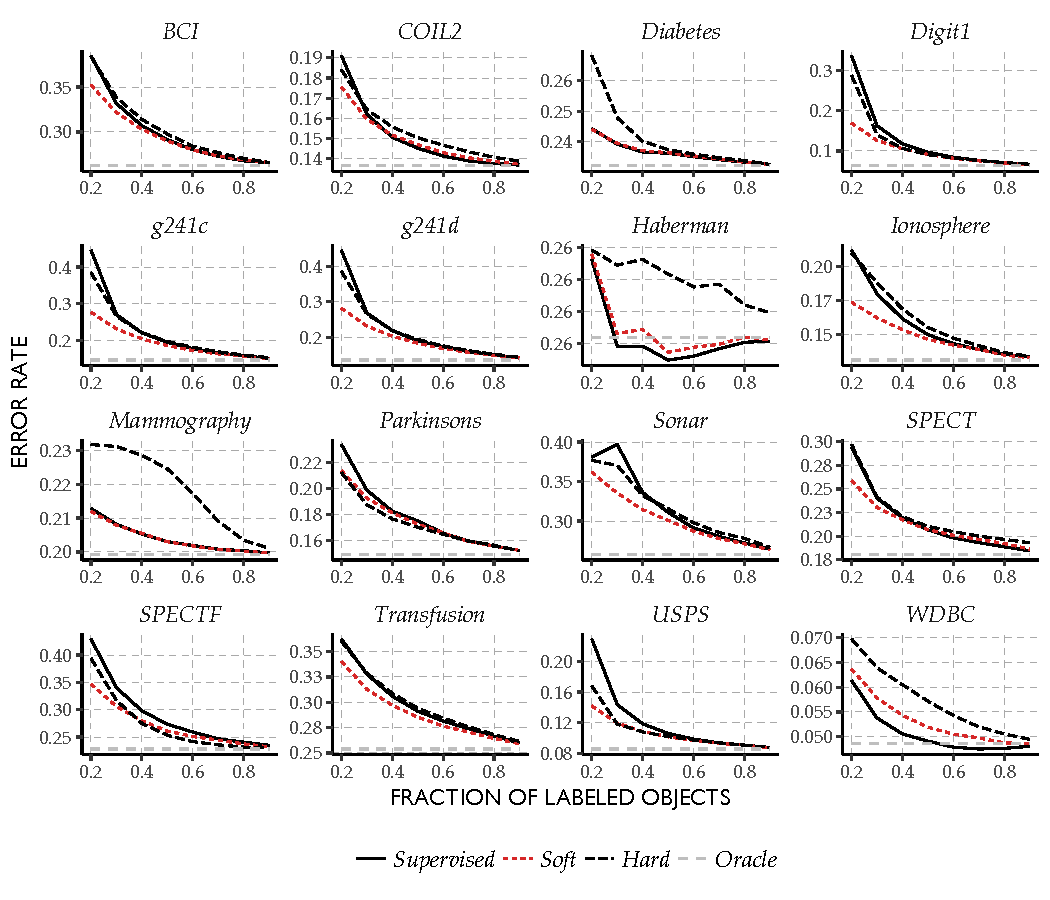
\includegraphics[width=\maxwidth]{figure/learningcurves-frac-1} \caption[Classification accuracy when different fractions of the training set are labeled]{Classification accuracy when different fractions of the training set are labeled. 20\% of the data is left out as test data, the fractions indicate the fraction of objects of the remaining data that was labeled. Oracle refers to the supervised classifier that has access to the labels of all the objects.}\label{fig:learningcurves-frac}
\end{figure*}


\end{knitrout}

\section{Discussion}
While reproducible research is sometimes framed as being a requirement for a result to be believable \citep{Goodman2016a,Donoho2009}, we think it is important to emphasize that it does not just benefit scientific discourse, but has advantages for the researchers carrying out the original work as well. We elaborate in what follows.

\subsection{Advantages to the Researcher}
Every research project is a collaboration. Sometimes with other individuals, but at the very least, a collaboration with yourself at some point in the future \cite[Ch. 13]{Donoho2009,Wickham2015}. It is rare that one does not have to revisit results after they were originally generated. Making results reproducible ensures that collaborators and you yourself in the future can easily get back into old results and make changes.

Secondly, although reproducibility does not eliminate all errors, it makes it easier to catch some type of errors. For instance, errors introduced by copying and pasting results from one document to another. At the very least, it makes it easier to fix them.

On the whole, for the individual researcher, reproducibility reduces friction: it makes it easy to make changes to figures and experiments even after the whole analysis is done since the later steps in an analysis can be reused if they are implemented in a reproducible way.

\subsection{Advantages to Scientific Communication}

\subsubsection{The Case for Reproducibility}
Unlike the claim by \citet{Patil2016}, the requirement of reproducibility is not something ``everybody agrees'' on. In this respect, \citet{Drummond2009}  argues that replicating results is an important part of scientific progress, yet exactly reproducing results is a poor substitute that does not add much other than counter outright fraud, and reproducibility can become a distraction. It may, in other words, not be worthwhile to spend much resources on. This is perhaps a bit too pessimistic, for two reasons. 

First, while reproducibility says nothing about the correctness of a result, it does allow apparent mistakes to be more easily checked than if the code was not available. Consider, for instance, the well-known case of the finding of \citet{Herndon2014}, after much work, that the conclusions in a highly influential study on the effect of government debt on economic growth depended on a data coding error and were very sensitive to particular choices in the analysis. While reproducibility does not eliminate these errors, nor was it required to finally spot them, it would likely have sped up the efforts to uncover these errors. As this case shows, this can have real world consequences, since the original conclusions had been used as an argument around the world by proponents of austerity measures during the recent economic crisis.

Secondly, Drummond's main concern is that reproducibility only deals with keeping steps in an analysis pipeline fixed, while replicability is about changing things. However, as the case study in this paper has hopefully shown, an important side effect from exactly reproducing results is that it removes friction for both the original researchers and the community to make changes and build on the code. We have seen this has two advantages: it aids in communicating results and insights and it provides a stepping stone for others to build new results on.

\subsubsection{Replicability in Pattern Recognition}
One way to define replicability is to consider a study where the ``same procedures are followed but new data are collected'' \cite{Goodman2016a}, where this data is sampled from the same population. Is this definition of replicability then a useful construct in methodological pattern recognition research? In the pattern recognition context, data from the same population may be hard to define, if your population is a set of benchmark datasets. One could wonder whether results generalize to other problems. This however, does not fall under the conventional definition of replicability, but rather under the term \emph{generalizability}. 
In most sciences, one of the things we learn from a replication is what the essential conditions are that are necessary for a result to hold. Analogously, we argue one aspect of replicability in pattern recognition research is the implementation of the methods. As we have noticed in our own work, it is an under appreciated point how difficult or easy it is for another programmer or analyst to replicate the results of a method. It teaches us not just something about the competence of the programmer (a point that is often overstated) but also of the elegance of the method and its sensitivity to particular implementation choices that may have gone unnoticed and even unreported in the original work.

\subsubsection{Practicalities}
There is still a technical problem with reproducible results: how do we make sure they are still reproducible after programming languages, toolboxes and online platforms change or cease to exist? For centuries, the unit of the paper as the narrative artefact has proven to be a format that stands the test of time and changes in technology. In the work considered here, we refer to papers from the 1950s, which we where able to recover and which got its authors' point across perfectly well. We need to ensure this is still the case for the work produced today. The only proposal we have towards this is that, at the very least, the software used to produce results is produced using open source software. This both allows one to dig into every level of the implementation if this is required to answer a particular question, but also provides some chance of ensuring software is still available in a future where a particular software vendor may have ceased to exist.

\subsubsection{Going Forward}
While we still consider reproducibility a worthwhile goal, there is a danger it leads to a false sense of security. Reproducibility is not replicability and it is replicability that constitutes progress in science. And reproducibility is not free: it requires effort on the part of the authors and reviewers of a manuscript. In the case covered in this paper, which is relatively easy to make reproducible, the advantages to the authors and the advantages to the community easily outweigh this effort. We should avoid dogmatism by realizing this trade-off might be different for other works.

\section{Conclusion}
We covered our approach to reproducing our paper on optimistic semi-supervised learning and showed some additional interesting, and nontrivial results by making slight adjustments to the figures and experiments which the reproducible nature of the paper allows. We argue that the advantages of reproducibility start during the research itself and extend to scientific communication. We need to realize, however, that reproducing results is not the same as replicating experiments, it primarily offers a poor but useful substitute.

\chapter{Semi-supervised Learning in R}
\chaptermark{Semi-supervised Learning in R}
\label{chapter:rssl}
\blfootnote{This chapter appeared as: Krijthe, J. H. 2016. RSSL: R package for Semi-supervised Learning. In B. Kerautret, M. Colom, \& P. Monasse (Eds.), Reproducible Research in Pattern Recognition. RRPR 2016. Lecture Notes in Computer Science, vol 10214. (pp. 104–115). Springer}

\begin{abstract}
In this paper, we introduce a package for semi-supervised learning research in the R programming language called RSSL. We cover the purpose of the package, the methods it includes and comment on their use and implementation. We then show, using several code examples, how the package can be used to replicate well-known results from the semi-supervised learning literature.
\end{abstract}



\section{Introduction}
Semi-supervised learning is concerned with using unlabeled examples, that is, examples for which we know the values for the input features but not the corresponding outcome, to improve the performance of supervised learning methods that only use labeled examples to train a model. An important motivation for investigations into these types of algorithms is that in some applications, gathering labels is relatively expensive or time-consuming, compared to the cost of obtaining an unlabeled example. Consider, for instance, building a web-page classifier. Downloading millions of unlabeled web-pages is easy. Reading them to assign a label is time-consuming. Effectively using unlabeled examples to improve supervised classifiers can therefore greatly reduce the cost of building a decently performing prediction model, or make it feasible in cases where labeling many examples is not a viable option.

While the R programming language \cite{RCoreTeam2016} offers a rich set of implementations of a plethora of supervised learning methods, brought together by machine learning packages such as \texttt{caret} and \texttt{mlr} there are fewer implementations of methods that can deal with the semi-supervised learning setting. This both impedes the spread of the use of these types of algorithms by practitioners, and makes it harder for researchers to study these approaches or compare new methods to existing ones.  The goal of the RSSL package is to make a step towards filling this hiatus, with a focus on providing methods that exemplify common behaviours of semi-supervised learning methods.

Until recently, no package providing multiple semi-supervised learning methods was available in R\footnote{Recently, the \texttt{SSL} package was introduced whose implementations are mostly complementary to those offered in our package: \url{https://CRAN.R-project.org/package=SSL}}. In other languages, semi-supervised learning libraries that bring together several different methods are not available either, although there are general purpose machine learning libraries, such as scikit-learn in Python \cite{scikit-learn} that offer implementations of some semi-supervised algorithms. A broader set of implementations is available for Matlab, since the original implementations provided by the authors of many of the approaches covered by our package are provided for Matlab. The goal of our package is to bring some of these implementations together in the R environment by providing common interfaces to these methods, either implementing these methods in R, translating code to R or providing interfaces to C++ libraries.

The goal of this work is to give an overview of the package and make some comments how it is implemented and how it can be used. We will then provide several examples on how the package can be used to replicate various well-known results from the semi-supervised learning literature.

\section{Overview of the Package}

\subsection{Classifiers}
The package focuses on semi-supervised classification. We give an overview of the classifiers that are available in \Cref{table:classifiers}. We consider it important to compare the performance of semi-supervised learners to their supervised counterparts. We therefore include several supervised implementations and sets of semi-supervised methods corresponding to each supervised method. Most of the methods are new implementations in R based on the description of the methods in the original research papers. For others, we either provide a (close to) direct translation of the original code into R code or an R interface to the original C++ code. For the latter we make use of the Rcpp package \cite{Eddelbuettel2011}. In some cases (WellSVM and S4VM) it was necessary to also include a customized version of LIBSVM \cite{Chang2011} on which these implementations depend.

A common wrapper method for semi-supervised learning, self-learning, is available for all supervised learners, since it merely requires a supervised classifier and some unlabeled objects. Other types of semi-supervised methods that are available for multiple supervised classifiers are the moment (or intrinsically) constrained methods of \citet{Loog2010,Loog2014a}, the implicitly constrained methods of \citet{Krijthe2014,Krijthe2017,Krijthe2017projection} and the Laplacian regularization of \citet{Belkin2006}.

All the classifier functions require as input either matrices with feature values (one for the labeled data and one for the unlabeled data) and a \texttt{factor} object containing the labels, or a \texttt{formula} object defining the names input and target variables and a corresponding \texttt{data.frame} object containing the whole dataset. In the examples, we will mostly use the latter style, since it fits better with the use of the pipe operator that is becoming popular in R programming.

Each classifier function returns an object of a specific subclass of the \texttt{Classifier} class containing the trained classifier. There are several methods that we can call on these objects. The \texttt{predict} method predicts the labels of new data. \texttt{decisionvalues} returns the value of the decision function for new objects. If available, the \texttt{loss} method returns the classifier specific loss (the surrogate loss used to train the classifier) incurred by the classifier on a set of examples. If the method assigns responsibilities --probabilities of belonging to a particular class-- to the unlabeled examples, \texttt{responsibilities} returns the responsibility values assigned to the unlabeled examples. For linear classifiers, we often provide the \texttt{line\_coefficients} method that provides the coefficients to plot a 2-dimensional decision boundary, which may be useful for plotting the classifier in simple 2D examples.

\begin{table}
\label{table:classifiers}
\caption{Overview of classifiers available in RSSL}
\begin{center}
\scriptsize
\begin{tabular}{ lcccl } 
 \toprule
 \textsc{Classifier} & \textsc{R} & \textsc{Interface} & \textsc{Port} & \textsc{Reference} \\ 
 \midrule
\textbf{(Kernel) Least Squares Classifier} & \checkmark &  &  & \cite{Hastie2009} \\
\, Implicitly Constrained  & \checkmark & & & \cite{Krijthe2017}  \\
\, Implicitly Constrained Projection  & \checkmark & & & \cite{Krijthe2017projection}  \\
\, Laplacian Regularized & \checkmark & & & \cite{Belkin2006} \\
\, Updated Second Moment & \checkmark & & & \cite{Shaffer1991}  \\
\, Self-learning & \checkmark & & & \cite{McLachlan1975} \\
\, Optimistic / ``Expectation Maximization'' & \checkmark & & & \cite{Krijthe2016a}  \\
\midrule
\textbf{Linear Discriminant Analysis} & \checkmark & & & \cite{Webb2002} \\
\, Expectation Maximization  & \checkmark & & & \cite{Dempster1977} \\
\, Implicitly Constrained  & \checkmark & & & \cite{Krijthe2014} \\
\, Maximum Constrastive Pessimistic  & & & \checkmark & \cite{Loog2016} \\
\, Moment Constrained  & \checkmark & & & \cite{Loog2014a} \\
\, Self-learning & \checkmark & & & \cite{McLachlan1975} \\
\midrule
\textbf{Nearest Mean Classifier} & \checkmark & & & \cite{Webb2002} \\
\, Expectation Maximization & \checkmark & & & \cite{Dempster1977} \\
\, Moment Constrained & \checkmark & & & \cite{Loog2010} \\
\, Self-learning & \checkmark & & & \cite{McLachlan1975} \\
\midrule
\textbf{Support Vector Machine} & \checkmark & & &  \\
\, SVMlin & & \checkmark & & \cite{Sindhwani2006} \\
\, WellSVM & & & \checkmark & \cite{Li2013} \\
\, S4VM & & & \checkmark & \cite{Li2015} \\
\, Transductive SVM (Convex Concave Procedure) & \checkmark & & & \cite{Collobert2006} \\
\, Laplacian SVM & \checkmark & & & \cite{Belkin2006} \\
\, Self-learning & \checkmark & & & \cite{McLachlan1975} \\
\midrule
\textbf{Logistic Regression} & \checkmark & & &  \\
\, Entropy Regularized Logistic Regression & \checkmark & & & \cite{Grandvalet2005} \\
\, Self-learning & \checkmark & & & \cite{McLachlan1975} \\
\midrule
Harmonic Energy Minimization & \checkmark & & & \cite{Zhu2003} \\
\bottomrule
\end{tabular}
\end{center}
\end{table}

\subsection{Utility Functions}
In addition to the implementations of the classifiers themselves, the package includes a number of functions that simplify setting up experiments and studying these classifiers. There are three main categories of functions: functions to generate simulated datasets, functions to evaluate classifiers and run experiments and functions for plotting trained classifiers.

\subsubsection{Generated Datasets}
A number of functions, of the form \texttt{generate*}, create datasets sampled from archetypical simulated problems. An overview of simulated datasets is given in \Cref{fig:generateddatasets}. You will notice that these datasets mostly show examples where the structure of the density of the feature values is either very informative or not informative at all for the estimation of the conditional distribution of the labels given the feature value. A major theme in semi-supervised learning research is how to leverage this connection between the distribution of the features and the conditional distribution of the labels, and what happens if this connection is non-existent. These simulated datasets offer some simple but interesting test cases for semi-supervised methods.
\begin{knitrout}
\definecolor{shadecolor}{rgb}{1, 1, 1}\color{fgcolor}\begin{figure}
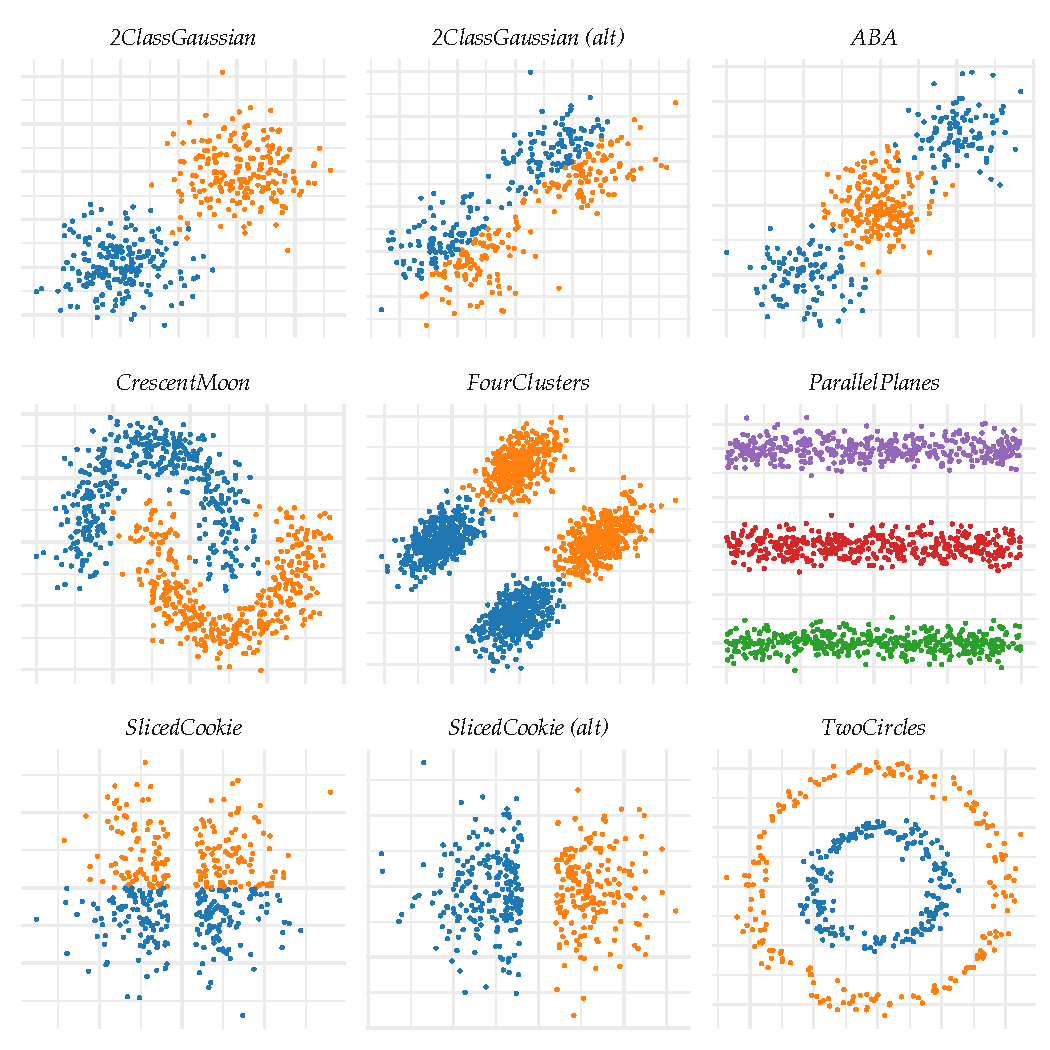
\includegraphics[width=\maxwidth]{figure/generateddatasets-1} \caption[Simulated Datasets]{Simulated Datasets. Each can be generated using a function of the form \texttt{generate*}, were \texttt{*} should be replaced by the name of the dataset. (alt) indicates non-default parameters where used when calling the function.}\label{fig:generateddatasets}
\end{figure}


\end{knitrout}

\subsubsection{Classifier Evaluation}
To evaluate the performance of different methods, the package contains three types of functions that implement standard procedures for setting up such experiments. The first is by splitting a fully labeled dataset into a labeled set, an unlabeled set and a test set. For data in the form of a matrix, the \texttt{split\_dataset\_ssl} can be used. For data in the form of a data frame, the easiest way is to use \texttt{magrittr}'s pipe operator, splitting the data using the \texttt{split\_random} command, using \texttt{add\_missinglabels\_mar} to randomly remove labels, and \texttt{missing\_labels} or \texttt{true\_labels} to recover these labels when we want to evaluate the performance on the unlabeled objects.
The second type of experiment is to apply cross-validation in a semi-supervised setting using \texttt{CrossValidationSSL}. Distinct from the normal cross-validation setting, the data in the training folds get randomly assigned to the labeled or unlabeled set.
The third type of experiment enabled by the package is to generate learning curves using the \texttt{LearningCurveSSL} function. These are performance curves for increasing numbers of unlabeled examples or an increasing fraction of labeled examples. 
For both the learning curves and cross-validation, multiple datasets can be given as input and the performance measures can be user defined, or one could use one of the supplied \texttt{measure\_*} functions. Also in both cases, the experiments can optionally be run in parallel on multiple cores to speed up computation.

\subsubsection{Plotting}
Three ways to plot classifiers in simple 2D examples are provided. The most general method relies on the ggplot2 package \cite{Wickham2009} to plot the data and is provided in the form of the \texttt{stat\_classifier} that can add  classification boundaries to \texttt{ggplot2} plots. \texttt{geom\_linearclassifier} works in a similar way, but only works for a number of linear classifiers that have an associated \texttt{line\_coefficients} method. Lastly, for these classifiers \texttt{line\_coefficients} can be used directly to get the parameters that define the linear decision boundary, for use in a custom plotting function. In the examples, we will illustrate the use of \texttt{stat\_classifier} and \texttt{geom\_linearclassifier}.

\section{Installation}
The package is available from the Comprehensive R Archive Network (CRAN). As such, the easiest way to install the package is to run the following command using a recent version of R:
\begin{knitrout}
\definecolor{shadecolor}{rgb}{1, 1, 1}\color{fgcolor}\begin{kframe}
\begin{alltt}
\hlkwd{install.packages}\hlstd{(}\hlstr{"RSSL"}\hlstd{)}
\end{alltt}
\end{kframe}
\end{knitrout}
\noindent The latest development version of the package can be installed using:
\begin{knitrout}
\definecolor{shadecolor}{rgb}{1, 1, 1}\color{fgcolor}\begin{kframe}
\begin{alltt}
\hlcom{# If devtools is not installed run: install.packages("devtools")}
\hlstd{devtools}\hlopt{::}\hlkwd{install_github}\hlstd{(}\hlstr{"jkrijthe/RSSL"}\hlstd{)}
\end{alltt}
\end{kframe}
\end{knitrout}

\section{Examples}
In this section, we will provide several examples of how the RSSL package can be used to illustrate or replicate results from the semi-supervised learning literature. Due to space constraints, we provide parts of the code for the examples in the text below. The complete code for all examples can be found in the source version of this document, which can be found on the author's website\footnote{\url{www.jessekrijthe.com}}.

\subsection{A Failure of Self-Learning}
While semi-supervised learning may seem to be obviously helpful, the fact that semi-supervised methods can actually lead to worse performance than their supervised counterparts has been both widely observed and described \cite{Cozman2003}. We will generate an example where unlabeled data is helpful (using the 2ClassGaussian problem from \Cref{fig:generateddatasets}) and one where unlabeled data actually leads to an increase in the classification error (2ClassGaussian (alt) in \Cref{fig:generateddatasets}), for the least squares classifier and self-learning as the semi-supervised learner. This can be done using the following code:
\begin{knitrout}
\definecolor{shadecolor}{rgb}{1, 1, 1}\color{fgcolor}\begin{kframe}
\begin{alltt}
\hlkwd{library}\hlstd{(RSSL)}
\hlkwd{set.seed}\hlstd{(}\hlnum{1}\hlstd{)}

\hlcom{# Set the datasets and corresponding formula objects}
\hlstd{datasets} \hlkwb{<-} \hlkwd{list}\hlstd{(}\hlstr{"2 Gaussian Expected"}\hlstd{=}
                   \hlkwd{generate2ClassGaussian}\hlstd{(}\hlkwc{n}\hlstd{=}\hlnum{2000}\hlstd{,}\hlkwc{d}\hlstd{=}\hlnum{2}\hlstd{,}\hlkwc{expected}\hlstd{=}\hlnum{TRUE}\hlstd{),}
                 \hlstr{"2 Gaussian Non-Expected"}\hlstd{=}
                   \hlkwd{generate2ClassGaussian}\hlstd{(}\hlkwc{n}\hlstd{=}\hlnum{2000}\hlstd{,}\hlkwc{d}\hlstd{=}\hlnum{2}\hlstd{,}\hlkwc{expected}\hlstd{=}\hlnum{FALSE}\hlstd{))}
\hlstd{formulae} \hlkwb{<-} \hlkwd{list}\hlstd{(}\hlstr{"2 Gaussian Expected"}\hlstd{=}\hlkwd{formula}\hlstd{(Class}\hlopt{~}\hlstd{.),}
                 \hlstr{"2 Gaussian Non-Expected"}\hlstd{=}\hlkwd{formula}\hlstd{(Class}\hlopt{~}\hlstd{.))}

\hlcom{# Define the classifiers to be used}
\hlstd{classifiers} \hlkwb{<-} \hlkwd{list}\hlstd{(}
  \hlstr{"Supervised"} \hlstd{=} \hlkwa{function}\hlstd{(}\hlkwc{X}\hlstd{,}\hlkwc{y}\hlstd{,}\hlkwc{X_u}\hlstd{,}\hlkwc{y_u}\hlstd{) \{} \hlkwd{LeastSquaresClassifier}\hlstd{(X,y)\},}
  \hlstr{"Self-learning"} \hlstd{=} \hlkwa{function}\hlstd{(}\hlkwc{X}\hlstd{,}\hlkwc{y}\hlstd{,}\hlkwc{X_u}\hlstd{,}\hlkwc{y_u}\hlstd{) \{}
                \hlkwd{SelfLearning}\hlstd{(X,y,X_u,}\hlkwc{method} \hlstd{= LeastSquaresClassifier)\})}

\hlcom{# Define the performance measures to be used and run experiment}
\hlstd{measures} \hlkwb{<-} \hlkwd{list}\hlstd{(}\hlstr{"Error"} \hlstd{=  measure_error,} \hlstr{"Loss"} \hlstd{= measure_losstest)}
\hlstd{results_lc} \hlkwb{<-} \hlkwd{LearningCurveSSL}\hlstd{(formulae,datasets,}
                           \hlkwc{classifiers}\hlstd{=classifiers,}
                           \hlkwc{measures}\hlstd{=measures,}\hlkwc{verbose}\hlstd{=}\hlnum{FALSE}\hlstd{,}
                           \hlkwc{repeats}\hlstd{=}\hlnum{100}\hlstd{,}\hlkwc{n_l}\hlstd{=}\hlnum{10}\hlstd{,}\hlkwc{sizes} \hlstd{=} \hlnum{2}\hlopt{^}\hlstd{(}\hlnum{1}\hlopt{:}\hlnum{10}\hlstd{))}
\end{alltt}
\end{kframe}
\end{knitrout}
\noindent When we plot these results (using the \texttt{plot} method and optionally changing the display settings of the plot), we get the figure shown in \Cref{fig:plot-lc}. What this shows is that, clearly, semi-supervised methods can be outperformed by their supervised counterpart for some datasets, for some choice of semi-supervised learner. Given that one may have little labeled training data to accurately detect that this is happening, in some settings we may want to consider methods that inherently attempt to avoid this deterioration in performance. We will return to this in a later example.

\begin{knitrout}
\definecolor{shadecolor}{rgb}{1, 1, 1}\color{fgcolor}\begin{figure}
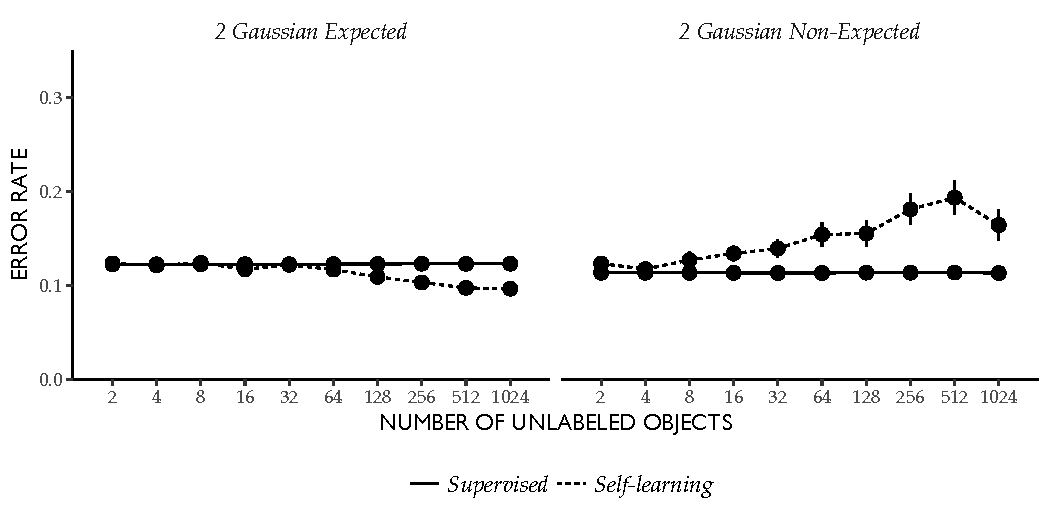
\includegraphics[width=\maxwidth]{figure/plot-lc-1} \caption{Example where self-learning leads to better performance as we add more unlabeled data (left) and increasingly worse performance as unlabeled data is added (right). The classifier used is the least squares classifier. The datasets are similar to the ones shown in \Cref{fig:generateddatasets}.}\label{fig:plot-lc}
\end{figure}


\end{knitrout}

\subsection{Graph Based Semi-supervised Learning}
Many methods in semi-supervised learning attempt to use the assumption that labels change smoothly over dense regions in the feature space. An early attempt to encode this assumption is offered by \cite{Zhu2003} who propose to minimize an energy function for the labels of the unlabeled objects that penalizes large deviations between labels assigned to objects that are close, for some measure of closeness. This so-called harmonic energy formulation can also be interpreted as a propagation of the labels from the labeled objects to the unlabeled objects, through a graph that encodes a measure of closeness. We recreate \cite{Zhu2003}'s Figure~2, which can be found in \Cref{fig:labelpropagation}. Due to space constraints, we will defer the code to the online version of this document, since it is similar to the code for the next example.
\begin{knitrout}
\definecolor{shadecolor}{rgb}{1, 1, 1}\color{fgcolor}\begin{figure}
\subfloat[Parallel planes dataset\label{fig:labelpropagation1}]{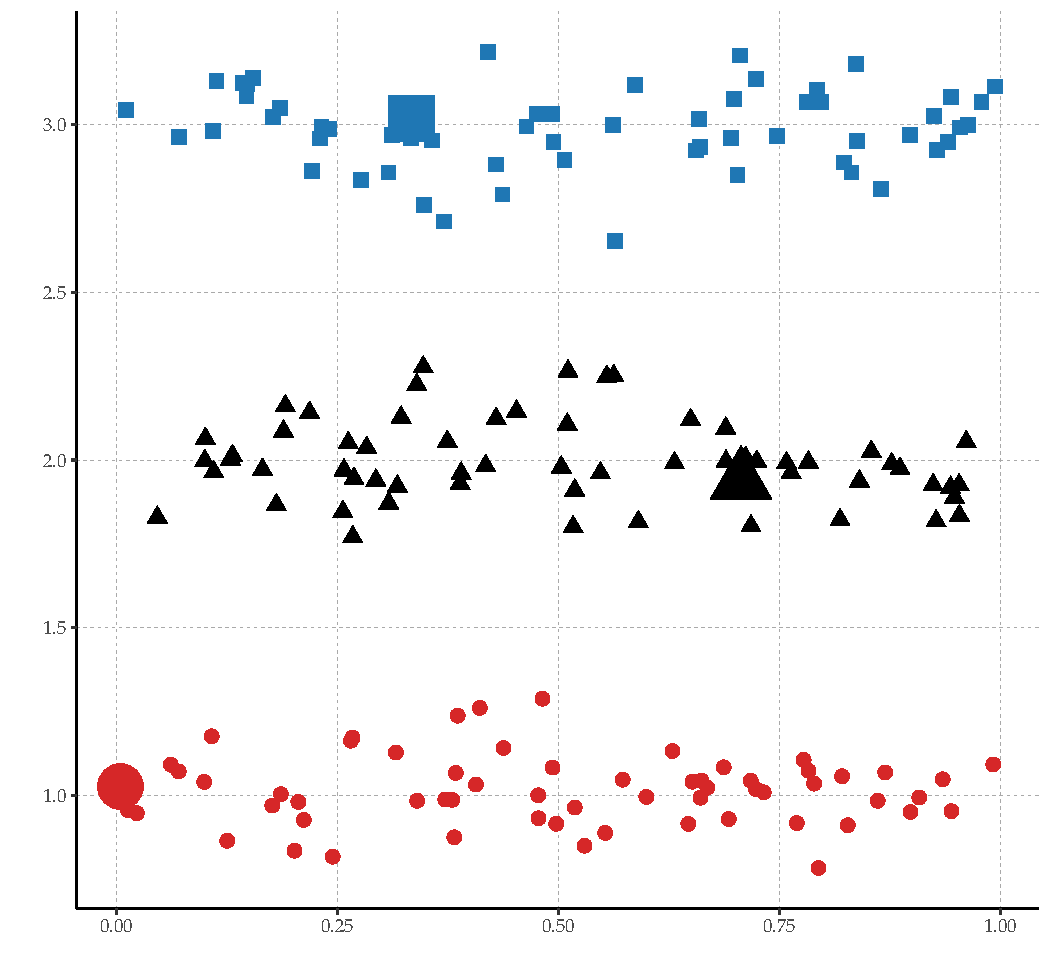
\includegraphics[width=.48\linewidth]{figure/labelpropagation-1} }
\subfloat[Spirals dataset\label{fig:labelpropagation2}]{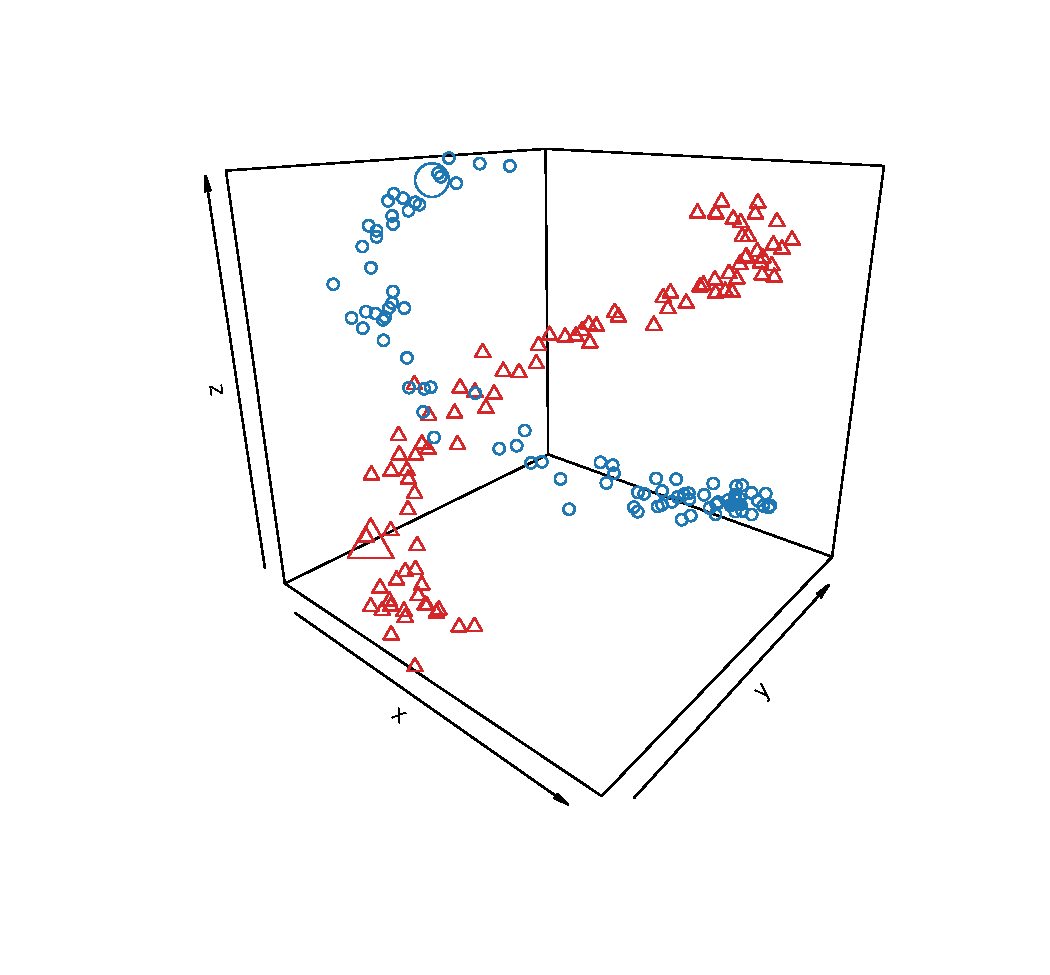
\includegraphics[width=.48\linewidth]{figure/labelpropagation-2} }\caption[Replication of Figure 2 from \cite{Zhu2003} demonstrating harmonic energy minimization]{Replication of Figure 2 from \cite{Zhu2003} demonstrating harmonic energy minimization. The larger points indicate the labeled objects. The color indicates the predicted class.}\label{fig:labelpropagation}
\end{figure}


\end{knitrout}

\subsection{Manifold Regularization}
Belkin et al. \cite{Belkin2006} build on the ideas of \cite{Zhu2003} by formulating the smoothness of the labeling function over the data manifold as a regularization term. In RSSL this Laplacian regularization term is included in both an SVM formulation and a regularized least squares formulation. For the Laplacian SVM formulation, Figure~2 from \cite{Belkin2006} provides an example of its performance on a simulated dataset. We can replicate this result using the following code. The results are shown in \Cref{fig:manifoldregularization}.
\begin{knitrout}
\definecolor{shadecolor}{rgb}{1, 1, 1}\color{fgcolor}\begin{kframe}
\begin{alltt}
\hlkwd{library}\hlstd{(RSSL)}
\hlkwd{library}\hlstd{(dplyr)}
\hlkwd{library}\hlstd{(ggplot2)}
\hlstd{plot_style} \hlkwb{<-} \hlkwd{theme_classic}\hlstd{()} \hlcom{# Set the style of the plot}

\hlkwd{set.seed}\hlstd{(}\hlnum{2}\hlstd{)}
\hlstd{df_unlabeled} \hlkwb{<-} \hlkwd{generateCrescentMoon}\hlstd{(}\hlkwc{n}\hlstd{=}\hlnum{100}\hlstd{,}\hlkwc{sigma} \hlstd{=} \hlnum{0.3}\hlstd{)} \hlopt
  \hlkwd{add_missinglabels_mar}\hlstd{(Class}\hlopt{~}\hlstd{.,}\hlkwc{prob}\hlstd{=}\hlnum{1}\hlstd{)}
\hlstd{df_labeled} \hlkwb{<-} \hlkwd{generateCrescentMoon}\hlstd{(}\hlkwc{n}\hlstd{=}\hlnum{1}\hlstd{,}\hlkwc{sigma} \hlstd{=} \hlnum{0.3}\hlstd{)}
\hlstd{df} \hlkwb{<-} \hlkwd{rbind}\hlstd{(df_unlabeled,df_labeled)}

\hlstd{c_svm} \hlkwb{<-} \hlkwd{SVM}\hlstd{(Class}\hlopt{~}\hlstd{.,df_labeled,}\hlkwc{scale}\hlstd{=}\hlnum{FALSE}\hlstd{,}
             \hlkwc{kernel} \hlstd{= kernlab}\hlopt{::}\hlkwd{rbfdot}\hlstd{(}\hlnum{0.05}\hlstd{),}
             \hlkwc{C}\hlstd{=}\hlnum{2500}\hlstd{)}

\hlstd{c_lapsvm1} \hlkwb{<-} \hlkwd{LaplacianSVM}\hlstd{(Class}\hlopt{~}\hlstd{.,df,}\hlkwc{scale}\hlstd{=}\hlnum{FALSE}\hlstd{,}
                         \hlkwc{kernel}\hlstd{=kernlab}\hlopt{::}\hlkwd{rbfdot}\hlstd{(}\hlnum{0.05}\hlstd{),}
                         \hlkwc{lambda} \hlstd{=} \hlnum{0.0001}\hlstd{,}\hlkwc{gamma}\hlstd{=}\hlnum{10}\hlstd{)}

\hlstd{c_lapsvm2} \hlkwb{<-} \hlkwd{LaplacianSVM}\hlstd{(Class}\hlopt{~}\hlstd{.,df,}\hlkwc{scale}\hlstd{=}\hlnum{FALSE}\hlstd{,}
                         \hlkwc{kernel}\hlstd{=kernlab}\hlopt{::}\hlkwd{rbfdot}\hlstd{(}\hlnum{0.05}\hlstd{),}
                         \hlkwc{lambda} \hlstd{=} \hlnum{0.0001}\hlstd{,}\hlkwc{gamma}\hlstd{=}\hlnum{10000}\hlstd{)}

\hlcom{# Plot the results }
\hlcom{# Change the arguments of stat_classifier to plot the Laplacian SVM}
\hlkwd{ggplot}\hlstd{(df_unlabeled,} \hlkwd{aes}\hlstd{(}\hlkwc{x}\hlstd{=X1,}\hlkwc{y}\hlstd{=X2))} \hlopt{+}
  \hlkwd{geom_point}\hlstd{()} \hlopt{+}
  \hlkwd{geom_point}\hlstd{(}\hlkwd{aes}\hlstd{(}\hlkwc{color}\hlstd{=Class,}\hlkwc{shape}\hlstd{=Class),}\hlkwc{data}\hlstd{=df_labeled,}\hlkwc{size}\hlstd{=}\hlnum{5}\hlstd{)} \hlopt{+}
  \hlkwd{stat_classifier}\hlstd{(}\hlkwc{classifiers}\hlstd{=}\hlkwd{list}\hlstd{(}\hlstr{"SVM"}\hlstd{=c_svm),}\hlkwc{color}\hlstd{=}\hlstr{"black"}\hlstd{)} \hlopt{+}
  \hlkwd{ggtitle}\hlstd{(}\hlstr{"SVM"}\hlstd{)}\hlopt{+}
  \hlstd{plot_style}
\end{alltt}
\end{kframe}\begin{figure}
\subfloat[$\lambda=0.0001$, $\gamma=0$\label{fig:manifoldregularization1}]{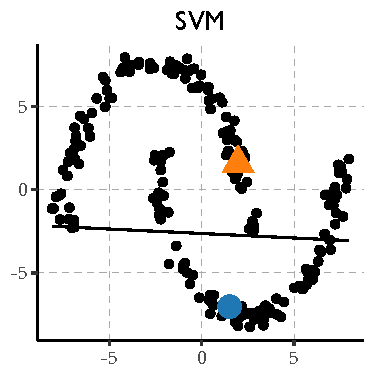
\includegraphics[width=0.32\linewidth]{figure/manifoldregularization-1} }
\subfloat[$\lambda=0.0001$, $\gamma=10$\label{fig:manifoldregularization2}]{\includegraphics[width=0.32\linewidth]{figure/manifoldregularization-2} }
\subfloat[$\lambda=0.0001$, $\gamma=10000$\label{fig:manifoldregularization3}]{\includegraphics[width=0.32\linewidth]{figure/manifoldregularization-3} }\caption[Replication of Figure~2 from \cite{Belkin2006}]{Replication of Figure~2 from \cite{Belkin2006}. Laplacian SVM for various values of the influence of the unlabeled data.}\label{fig:manifoldregularization}
\end{figure}


\end{knitrout}

\subsection{Low Density Separation}
A number of semi-supervised approaches attempt to leverage the assumption that the classification boundary may reside in a region of low-density. The Semi-supervised SVM or Transductive SVM \cite{Joachims1999} is one such approach. In \cite[Chapter 6]{Zhu2009}, an example is given for the potential problems this low-density assumption may cause when it is not valid by considering two artificial datasets. Here we replicate these results for a different classifier that makes use of the low-density assumption: entropy regularized logistic regression \cite{Grandvalet2005}. The results are shown in \Cref{fig:lowdensityproblem}. The code to generate these results can be found in the source version of this document.
\begin{knitrout}
\definecolor{shadecolor}{rgb}{1, 1, 1}\color{fgcolor}\begin{figure}
\subfloat[Low-density assumption\label{fig:lowdensityproblem1}]{\includegraphics[width=.49\linewidth]{figure/lowdensityproblem-1} }
\subfloat[Non low-density assumption\label{fig:lowdensityproblem2}]{\includegraphics[width=.49\linewidth]{figure/lowdensityproblem-2} }\caption[Demonstration of potential problems when the low density assumption does not hold, similar to Figure 6.5 in \cite{Zhu2009}]{Demonstration of potential problems when the low density assumption does not hold, similar to Figure 6.5 in \cite{Zhu2009}}\label{fig:lowdensityproblem}
\end{figure}


\end{knitrout}


\subsection{Improvement Guarantees}
We now return to the example of deterioration in performance from \Cref{fig:plot-lc}. The goal of our work in \cite{Loog2016,Krijthe2016a,Krijthe2017} is to construct methods that are guaranteed to outperform the supervised alternative. The guarantee that is given in these works is that the semi-supervised learner outperforms the supervised learner on the full, labeled and unlabeled, training set in terms of the surrogate loss (cf. \cite{Loog2014b}). The following code trains semi-supervised classifiers in these cases and returns the mean loss on the whole training set, the output is shown below the code example. It shows that indeed, these methods do not deteriorate performance in terms of the surrogate loss, while the self-learning method does show this deterioration in performance.
\begin{knitrout}
\definecolor{shadecolor}{rgb}{1, 1, 1}\color{fgcolor}\begin{kframe}
\begin{alltt}
\hlkwd{library}\hlstd{(RSSL)}
\hlkwd{set.seed}\hlstd{(}\hlnum{1}\hlstd{)}

\hlcom{# Generate Example}
\hlstd{df} \hlkwb{<-} \hlkwd{generate2ClassGaussian}\hlstd{(}\hlkwc{n}\hlstd{=}\hlnum{1000}\hlstd{,} \hlkwc{d}\hlstd{=}\hlnum{2}\hlstd{,} \hlkwc{expected}\hlstd{=}\hlnum{FALSE}\hlstd{)}
\hlstd{df_semi} \hlkwb{<-} \hlkwd{add_missinglabels_mar}\hlstd{(df, Class}\hlopt{~}\hlstd{.,} \hlkwc{prob}\hlstd{=}\hlnum{0.995}\hlstd{)}

\hlcom{# Train and evaluate classifiers}
\hlkwd{mean}\hlstd{(}\hlkwd{loss}\hlstd{(}\hlkwd{LeastSquaresClassifier}\hlstd{(Class}\hlopt{~}\hlstd{.,df_semi),df))}
\hlkwd{mean}\hlstd{(}\hlkwd{loss}\hlstd{(}\hlkwd{SelfLearning}\hlstd{(Class}\hlopt{~}\hlstd{.,df_semi,}
                        \hlkwc{method}\hlstd{=LeastSquaresClassifier),df))}
\hlkwd{mean}\hlstd{(}\hlkwd{loss}\hlstd{(}\hlkwd{ICLeastSquaresClassifier}\hlstd{(Class}\hlopt{~}\hlstd{.,df_semi),df))}
\hlkwd{mean}\hlstd{(}\hlkwd{loss}\hlstd{(}\hlkwd{ICLeastSquaresClassifier}\hlstd{(Class}\hlopt{~}\hlstd{.,df_semi,}
                          \hlkwc{projection}\hlstd{=}\hlstr{"semisupervised"}\hlstd{),df))}
\end{alltt}
\begin{verbatim}
## [1] 0.1763921
## [1] 0.4813863
## [1] 0.1185772
## [1] 0.1236701
\end{verbatim}
\end{kframe}
\end{knitrout}


\section{Conclusion}
We presented RSSL, a package containing implementations and interfaces to implementations of semi-supervised classifiers, and utility methods to carry out experiments using these methods. We demonstrated how the package can be used to replicate several results from the semi-supervised learning literature. More usage examples can be found in the package documentation. We hope the package inspires practitioners to consider semi-supervised learning in their work and we invite others to contribute to and use the package for research. Moreover, we hope the package contributes towards making semi-supervised learning research, and the research of those who use these methods in an applied setting, fully reproducible.

\backmatter

\addtocontents{toc}{\vspace{\normalbaselineskip}}



\chapter[Discussion]{Discussion}

Given the increasing amounts of available (unlabeled) data, semi-supervised learning is an important practical problem. What is more, it is an interesting theoretical problem because it gets at the heart of the value of different types of information in estimating statistical models. The results in the previous chapters contribute to a better understanding of the limits of semi-supervised learning as well as introduce robust methods that guarantee improvements over the supervised alternative. In this final part of the thesis, let us revisit the main findings in the broader perspective of the research questions considered in the introduction.

\section{Semi-supervised Learning without Additional Assumptions}
One of the basic tenets in semi-supervised learning research has been that learning without additional assumptions about the relationship between $p_X$ and $p_{Y|X}$ is impossible. The results in \Cref{chapter:icls,chapter:iclda,chapter:projection,chapter:marginbased} nuance this view. For some supervised classifiers, guaranteed improvements are possible in terms of the surrogate loss on the labeled and unlabeled data. For other supervised methods, these guarantees are essentially impossible. To us, this suggests that taking into account the way supervised models are fitted, and recognizing the finite sample available, leads to different views on the possibilities of semi-supervised learning than considering models that are correctly specified. In practice, models are never perfect, and unlabeled data can be one way to correct some of these imperfections.

\section{Improvement Guarantees}
The improvement guarantees that we offer in \Cref{chapter:projection} are the first of their kind: they guarantee performance will not degrade for any possible labeling of the unlabeled data. The setting considered, however, does not necessarily correspond to generalization performance in terms of the error rate. 

Firstly, we make a claim about performance on the labeled and unlabeled data, rather than some unseen test set. In case the size of the unlabeled set grows to infinity, this guarantee converges to a generalization guarantee. Alternatively, the results can be adapted to the transductive setting where one is interested in predictions on a specific unlabeled set of objects. 

Nonetheless, it is interesting that we never use the assumption that the unlabeled data originate from the same distribution as the labeled data. A way forward to get to more general guarantees is to take this assumption into account while letting go of the requirement that the supervised solution is not better than the semi-supervised solution for every possible dataset with probability one.

A second property of the improvement guarantee considered in this work is that it is in terms of the surrogate loss of the supervised classifier. The reason we think this makes an interesting guarantee is two fold. For one, it guarantees that we construct a true semi-supervised version of the supervised classifier by ensuring we do well in terms of the criterion we would be optimizing if we did have the labels of the unlabeled objects. Secondly, for some of the supervised models, even for increasing  numbers of \emph{labeled} objects we can not guarantee classification performance increases, while they do improve in terms of the surrogate loss. ``Improving'' a classifier using unlabeled data should, therefore, be evaluated in terms of this measure, or the improved procedure is best considered a totally different method than the original supervised procedure.

It is important to consider what the improvement guarantee means for the loss for specific objects in the unlabeled set. Especially in the presence of outliers, a change in the classifier can lead to a higher loss for almost every observation, except for a few observations where the loss is reduced by a large amount. This is a consequence of considering the loss on all objects together, and has an effect similar to what one observes in James-Stein estimators \citep{Efron1977}, where these estimators dominate estimators that do not consider the loss on all objects simultaneously.

Instead of the surrogate loss, one could only be interested in getting improved classification performance. As mentioned, even in the supervised case, we do not minimize this loss directly. The goal in this thesis is to construct semi-supervised versions of common supervised procedures that are guaranteed to not perform worse. Since these supervised procedures consider surrogate losses, it makes sense to consider these same losses in the semi-supervised case. We may still be able to get performance guarantees in terms of the classification error through generalization bounds, similar to the supervised setting. While we guarantee performance improvements for any number of labeled objects, the effect of the unlabeled data may diminish as more labeled examples are added. As such, unlabeled data may have no effect on the convergence rate, as conjectured by \cite{Ben-David2008}. 

\section{On the Impossibility of Safe Semi-supervised Learning}
For a number of common supervised methods, the results in \Cref{chapter:marginbased} show that our notion of safe semi-supervised learning is inherently impossible. This is contrary to earlier claims for some of these models, such as for the support vector machine \cite{Li2015}. Our definition of safety, is conservatively strict: the supervised solution has to not be better than the semi-supervised procedure for any possible labeling of the unlabeled data. Compare this to the claim of \citet{Li2015} where this only has to hold for a labeling that is generated by a low-density separator. The claim we make is that, true safety concerns all possible contingencies, and this type of semi-supervised learning may well be impossible, in line with what others have claimed. It is all the more surprising, then, that for some classifiers, this notion of safety does lead to useful semi-supervised procedures.

\section{Thoughts on the Least Squares Classifier}
The reasons for measuring performance in terms of the surrogate loss have been outlined above. But in the thesis, we often considered one particular surrogate loss: the squared loss. This loss allowed us to derive simple, convex problems to obtain the semi-supervised estimator with interesting performance guarantees. These improvements, however, might only tell us something about the squared loss, and not about the classification problem we are trying to solve at all. One particular property of the squared loss is that the loss for an object may increase if the magnitude of the decision function is increased even when the object is correctly classified. Any improvements that we get, therefore, might ``improve'' the decision function in ways that have little to do with the classification problem. Furthermore, as we saw in the chapter on peaking, the least squares classifier can behave erratically when we have only little data compared to the number of features. The gains in classification performance that we do observe empirically, may just be because of the slight regularizing effect that the semi-supervised procedure has on a very unstable classifier. Nevertheless, this improvement is \emph{guaranteed}, and it is more than we might have been able to hope for, given the extremely strict conditions under which we consider safe improvements.

\section{Projections and Minimax Principles}
Within the projection framework we showed in \Cref{chapter:marginbased} that for many supervised methods the constraint set is basically too large to put any useful constraint on the semi-supervised solution. Leaving this issue of the size of the constraint set aside for now, there is the additional question what distance measure should be employed for losses other than the squared loss. This measure is important since it not only determines what semi-supervised solution is selected by determining the closest solution to the supervised solution within the constraint set, but also determines in what sense we are closer to the oracle solution. As of yet, we have no definite suggestion on how this should be solved. Initially, for some models, one might expect the KL-divergence to be a promising candidate. Unfortunately, the simple proof in \Cref{chapter:projection} does not directly apply in that case, since it is not a proper distance metric. 

An answer may be found in an equivalent (for the least squares case) formulation proposed by \citet{Loog2016}. One can show the projection is equivalent to finding the solution that minimizes the difference in loss between the supervised and semi-supervised solutions over all possible assignments of responsibilities of unlabeled objects to classes. For similar connections in a different problem see \citet{Arnold2000}. By using this minimax formulation for other classifiers and finding a distance measure that (approximately) leads to the same optimization problem, we may be able to generalize the projection procedure to other losses.

It is important to note that the novelty of the projection procedure proposed here is not in finding some solution within the constraint set -- self-learning, by definition, does this as well -- but by defining which solution to select from the set and the properties that follow. For instance, looking at the problem from the viewpoint of projections suggests how to improve semi-supervised estimators for which the implicit constraints are too loose. It suggests the constraint space is too large and we should somehow decrease its size. This has some correspondence with the basic intuition behind many semi-supervised approaches covered in the introduction which assume the unlabeled data limit the hypotheses that should be considered. A nice property of the implicit constraints is that they are guaranteed to contain the solution corresponding to the true labeling, which in turn can guarantee non-degradation of the semi-supervised estimator. But letting go of our strict notion of non-degradation, one could construct constraint sets that contain the oracle with high probability, but which are much smaller than the implicit constraints set. In experiments we conducted, assuming information about the proportion of objects of each class did not lead to large improvements in performance, but other such assumptions might.

One of the nice properties of the squared loss is that it leads to a closed form solution if we know the labels. This, in turn, leads to an efficient way to move through the constraint set to calculate the projection. For other losses this may be more difficult to achieve, but using tools like the implicit function theorem to deal with the constraints, one may still be able to find a reasonable formulation of the problem. In general, however, the computation of the projection does not scale well in terms of the number of unlabeled examples. Approximations to the constraint set may alleviate some of the computational burden without introducing a high probability of lowering performance.

\section{Semi-supervised Learning in Practice}
While the results in this thesis offer both insights into the semi-supervised learning problem and methods that guarantee performance improvements, in practice, we might be willing to forego some of this certainty if this means we might get large improvements in performance for many problems. We will first consider whether performance degradation is actually a problem and then make some comments about the future of semi-supervised learning in machine learning research and practice. 

\subsection{Conservatism}
In this thesis, we have taken an extremely conservative view to semi-supervised learning: because the semi-supervised solution might lead to worse performance than the supervised solution, we should explicitly construct methods that guard against this.

One of the reasons for considering these types of methods is that it may be hard to detect when semi-supervised learning is failing and fall back on a supervised methods, especially given the limited amounts of labeled data available. Many semi-supervised methods have been developed and shown to be effective by illustrating performance improvements for the most effective settings of the hyperparameters that are introduced, when effectiveness is evaluated based on the test set. This is not how one can apply these methods in practice, however, where hyperparameters and algorithms have to be selected based on the data at hand. We do not have a good grasp of how big this selection problem is in practice. How often will the wrong setting be selected and result in decreased performance? A big step forward to answer this question would be a large scale study over both datasets and methods to characterize the size of this problem, or whether it is a problem at all. One attempt has been made by \citet{Goldberg2009}, for two semi-supervised methods, which suggests the semi-supervised methods outperform the supervised method in the majority of cases when the hyperparameters are selected using cross-validation, but still lead to degradations in performance on a significant number of occasions. Studying this for a broader set of methods and datasets will give us some indication whether conservatism is mostly theoretically interesting or a practical necessity.

\subsection{Automatically Correct Methods}
This classifier selection problem also relates to the goal of constructing conservative methods: our ultimate goal is to construct methods that work ``automatically'', just like in the supervised case, where adding more data typically leads to better decision functions, or understand when this is not possible. As of yet, it is unclear whether this can also be achieved through some cross-validation strategy. Yet, even if it could, having methods automatically ensure this property has both advantages in understanding the limits of these methods, as shown in this thesis, and possible computational advantages.

\subsection{Violations of Basic Conditions}
As we noted in the introduction of this thesis, in semi-supervised learning it is assumed that the labels are missing at random. This means that the unlabeled data is assumed to come from a distribution that is identically to the distribution generating the labeled examples, when we integrate over the the label. In many settings, this is not a realistic assumption. Unlabeled data may be used because they were easy to gather and this type of convenience sampling may introduce biases in the type of data that are gathered. Consider, for instance, the example of gathering documents downloaded from the web to improve the performance of a system that attempts to classify newspaper articles. The two underlying distributions are likely to be different. Biases may also be introduced through the labeling of objects, even if the objects themselves originate from some i.i.d. process. This could happen if objects with certain labels are easier to label than others, and therefore more likely to be labeled. 

Because the assumption of the identical distribution of the unlabeled data is in many cases not realistic, the semi-supervised learning setting is often an idealized version of the actual problem that needs to be solved. Related learning settings cover scenarios where we do take violations of this assumption into account. In general, we can often describe these settings as \emph{transfer learning} problems \cite{torrey2009transfer, Quinonero-Candela2009}, where the data which one learns from do not come from the distribution on which the final classifier will be applied. More specifically, when the unlabeled data come from the target distribution we are interested in, this is known as \emph{domain adaptation} \citep{Kouw2016,Cortes2011}.

One can expect these related learning settings to require even more prior information than the more restricted semi-supervised setting, since we somehow have to model the relationship between the labeled and the unlabeled distribution as well as learn from the unlabeled data. The projected estimators framework presented in this thesis can, in principle, be adapted to some of these related learning settings as well. As of yet, it is unclear how effective this will be. For instance, in the domain adaptation setting, on the one hand, the regular supervised solution may be expected to perform poorly, leading to potential large improvements when using the projected estimator. On the other hand, the conservative nature of this estimator may not lead to large improvements because substantive prior assumptions are likely needed to model the transfer between domains.

Overall, it is worthwhile to keep in mind that the semi-supervised problem may be an idealized version of the problem we face in many applications. The insights gained by studying the semi-supervised setting could be extended to scenarios where we make more appropriate assumptions about the process that led us to observe the labeled and unlabeled datasets.

\subsection{The Reinvention of Self-Learning}
Handling missing data in general and semi-supervised learning in particular is not a new problem \citep{Little2002}. In \Cref{chapter:optimistic} we have covered methods going back to the 1930s that implement some form of self-learning in the context of missing outcomes. Many procedures, in one form or another, use this general concept by using imputation steps for the unlabeled data, followed by optimization steps, to find a semi-supervised solution. Expectation Maximization \cite{Dempster1977} can be considered in this light, but also some approaches to solving Transductive SVMs \citep{Joachims1999}. Many graph based approaches can also be considered in this way \citep{Zhu2003}, where labels are propagated over the graph. What these approaches have in common is that the labels are treated as missing variables in an optimization function and the main problem is finding their value that minimizes this objective. This thesis has shown that alternatives are possible, by not including an additional term in the objective function, but rather using the unlabeled data in different ways, such as formulating constraints on the solution.

Reinventing self-learning and renaming it in the process has become somewhat of a tradition in semi-supervised learning research. So much so that, to some, semi-supervised learning has become synonymous to self-learning. Among others, self-learning is known in the literature as self-training \citep{Zhu2005}, Baum-Welch reestimation \citep{Elworthy1994}, Yarowsky's algorithm and more recently, pseudo-labeling \cite{Lee2013}.

While this is not a problem in and of itself, it is important to heed the lessons we learned in the past and resist the dream of thinking these unlabeled data will automatically be as valuable as labeled examples, or that they will be a panacea for all problems. If anything, this thesis shows getting the full use out of these data often requires modelling and making assumptions. After all, statistical machine learning is as much about the model, as it is about the data.

\subsection{The New Frontier}
While many issues remain, it is encouraging to see semi-supervised methods  are starting to get used on large scale problems \cite{Ravi2016}. Some of the assumptions discussed in the introduction appear to be useful in these real-world applications, using enormous amounts of unlabeled data. Moreover, semi-supervised learning research is not immune to the recent advances in effectively learning hierarchical architectures. Advances are being made by sharing properties of networks that learn to reconstruct inputs and networks that predict labels from inputs \cite{Rasmus2015} which suggests something akin to the manifold assumption is effective in their application domain. Or by learning to distinguish between the unlabeled objects and generated objects that are similar to but not like the classes we are trying to learn using generative adversarial networks \cite{Salimans2016}. These and other approaches have shown promising performance on image recognition tasks, using relatively few labeled objects. 

While the models are becoming more complex, the basic questions still remain the same. For what problems does this work and why? What assumptions do we need to make to guarantee the unlabeled data are useful? And why is it essentially impossible to do this for some problems and models and possible for others? Steps have been made in these areas, but leaps still remain.

\section{From Reproducibility to Replicability}
In part three of the thesis, we covered the reproducibility of results in the context of the research that we did in the chapters prior. We argued that reproducibility is important, and often requires little extra effort, or even a reduction in effort to the researcher, while having various advantages in scientific communication. Yet, we noted that ultimately the goal is replicability: being able to produce the same qualitative findings from scratch. We are aware the definitions we used in these chapters are but a starting point and are glad to see developments to make these more concrete. The issues are becoming especially pertinent for research involving large models trained on enormous datasets, where the financial or time investment of reproducing results can be prohibitive. While scientific communication is built on trust, it is also requires an ability to operationalize skepticism by reproducing and replicating claims. How we will deal with this as a scientific community is an open problem.

\section{On Conceptual Research}
Lastly, let me comment on the type of research project that the work presented in the prior chapters represents. As you might have noticed, it contains a small number of important theorems but no long, complex proofs. It presents interesting new approaches, but no large complex models. It presents experiments on archetypical simulated datasets and well-known benchmark datasets but no `state-of-the-art' results on groundbreaking new problems. And in doing so, I hope that most of all, it contains an interesting new perspective on the problem of semi-supervised learning. Rather than theoretical research, whose implications can be hard to relate to practice, or applied research, which can be too focused on the details of the problem at hand, the work in this thesis represents what I would refer to as conceptual research in pattern recognition. Many have noted the large gap between theory and practice in semi-supervised learning. We hope to have contributed to this fascinating topic. But many questions remain. Apart from the answering some questions about semi-supervised learning and bringing up new ones, I hope to have gotten across that as with many problems in machine learning, statistics and pattern recognition, the issues are not just computational, but statistical, conceptual and sometimes even epistemological in nature. The work has given me a better understanding of the problem of semi-supervised learning, and I hope to have gotten these insights across in this thesis.


\scriptsize{\printbibliography[heading=bibintoc,title={References}]}

\normalsize
\chapter{Summary}
{\LARGE{\textsf{\MakeUppercase{Robust Semi-supervised Learning}}}}
\\[12pt]
Through advances in sensor, storage and communication technology and adoption of digital technology in every aspect of our lives, large amounts of data are routinely gathered. Statistical learning from data, in many cases, requires a specific type of datum: \emph{labeled} examples for which we know both the input and some outcome we would like to predict. The problem of semi-supervised learning is how to use, increasingly abundantly available, \emph{unlabeled} examples to improve supervised learning methods that typically only consider labeled examples.

One of the issues of semi-supervised learning methods is that adding unlabeled data, unlike our experience in the supervised paradigm, does not guarantee improved performance, nor do we understand very well when semi-supervised learning will be helpful. \emph{Robust} or \emph{safe} semi-supervised methods are those that attempt to ensure performance of a semi-supervised method is at least as good as its supervised counterpart. 

It is often assumed particular assumptions need to be made to allow for semi-supervised learning to be possible at all. Yet these assumptions may also be the cause of a decrease in performance. The main claim brought forth by this thesis is that, by avoiding these assumptions, for some classifiers, it it possible to construct robust semi-supervised classifiers, when we consider performance in terms of the so-called surrogate loss that the supervised classifier is optimizing and we measure performance on the labeled and unlabeled data. We also consider, for the class of classifiers defined by a margin-based loss function, under what conditions such improvements are possible, and for which methods such improvements are inherently impossible to obtain.

In the first part of this thesis, we show that by implicitly considering all possible labelings of the unlabeled data and the corresponding classifiers, and projecting the supervised solution unto this set of solutions, it is possible to construct a semi-supervised version of the least squares classifier, which, under strict theoretical conditions can be considered safe. We apply the same framework to linear discriminant analysis to show this idea can also be applied to other classifiers. Subsequently, by changing the distance measure used in the projection, we construct a procedure for the least squares classifier that is guaranteed to improve performance under much weaker conditions. This is the first method for which such strict improvement guarantees can be provided.

In practice, the performance of classification models is often evaluated in terms of the classification error, area under the ROC curve, F-score or other measures that consider the number of mistakes the classifier makes in one way or the other. On the other hand, the guarantees given in Part One of this thesis are in terms of the surrogate loss of a classifier. In Part Two, we consider these surrogate losses to show that they are interesting quantifies to study in their own right. We then prove it is impossible to construct any semi-supervised learner that guarantees the strong notion of robust/safe semi-supervised learning from Part One for a large class of common supervised algorithms defined by monotonically decreasing margin-based loss functions. This sheds additional light on the (im)possibilities of semi-supervised learning in general, and safe semi-supervised learning in particular.

Continuing with the squared loss of Part One, we construct a simple formulation of the well-known self-learning approach to semi-supervised learning, for the least squares classifier. A slight adaptation of this formulation leads to a type of soft-label self-learning which is shown to outperform the hard-label self-learning variant in many cases. While for these self-learning methods there are no safety guarantees, such as for the methods in Part One, these ideas are often applied in practice, and we show how this can be properly formulated and analyzed for the least squares classifier.

In some of the experiments carried out in this thesis, we find that a peaking phenomenon occurs. This is known to occur for some supervised classifiers, where, when there are fewer training examples than features, the error first increases as we add more data before it decreases again. We observe that a similar phenomenon occurs in the semi-supervised setting in a more extreme form. We argue the difference in severity between the supervised and semi-supervised setting can be explained by a lack of updating of the estimate of the class means while the intrinsic dimensionality of the problem grows. We also consider under what conditions the semi-supervised classifier recovers from the bad performance at the peak, as we add more unlabeled data.

Finally, in Part Three, we cover the reproducibility and replicability of the results uncovered in the course of this research programme and in pattern recognition research in general. We argue that reproducibility has many advantages which often outweigh the cost, but that this should not lead to complacency about replicating results, which in pattern recognition research, often means re-implementing methods. Additionally, we introduce a software package that can be used to reproduce the results presented in this thesis, and to replicate various well-known results in the semi-supervised learning.

Overall, the result of the work covered in this thesis is a new look at the possibilities and impossibilities for (robust) semi-supervised learning, and a novel perspective on using projections of estimators to construct these methods. As statistical learning starts to pervade many parts society, and unlabeled data become increasingly available, making use of this data and understanding its possibilities and limitations remains an important topic. As statistical models become more complex, the basic questions remain the same, questions whose answers we hope to have contributed to in this work.

\begin{otherlanguage}{dutch}
\chapter{Samenvatting}
{\LARGE{\textsf{\MakeUppercase{Robuust Semi-begeleid Leren}}}}
\\[12pt]
Door vooruitgang in technologie voor het meten, opslaan en delen van gegevens en door de toepassing van digitale technologie in alle facetten van ons leven, worden grote hoeveelheden gegevens op grote schaal verzameld. Om hier statistisch van te kunnen leren is een specifiek soort gegevens nodig: gelabelde voorbeelden waarvan de invoer en de gewenste uitkomst die we willen voorspellen bekend is. De uitdaging van semi-begeleid leren is hoe ongelabelde voorbeelden, die in steeds grotere hoeveelheden beschikbaar zijn, gebruikt kunnen worden om methoden voor begeleid leren, die typisch enkel leren van gelabelde voorbeelden, te verbeteren.

Een van de problemen met semi-begeleide methoden is dat het toevoegen van ongelabelde voorbeelden niet altijd leidt tot een verbetering van de resultaten, in tegenstelling tot begeleid leren. Bovendien is er beperkt begrip over in welke situaties semi-begeleide methoden wel werken. \emph{Robuuste} of \emph{Veilige} semi-begeleide methoden zijn methoden die een garantie proberen te geven dat de prestaties van een semi-begeleid algoritme minstens zo goed zijn als die van zijn (volledig-)begeleide tegenhanger.

Er wordt vaak aangenomen dat specifieke vooronderstellingen nodig zijn om semi-begeleid leren mogelijk te maken. Deze vooronderstellingen zijn tevens een mogelijke oorzaak voor de slechtere resultaten. De voornaamste stelling in dit proefschrift is dat het, door het vermijden van deze aannames, mogelijk is om robuuste semi-begeleide classificatie algoritmen te construeren. Hierbij meten we de prestaties van een algoritme in termen van een zogenaamde surrogaat verliesfunctie die door een begeleid classificatie algoritme wordt geoptimaliseerd en meten de prestaties op de gelabelde en ongelabelde voorbeelden. Naast de constructie van dergelijke robuuste algoritmen laten we zien onder welke voorwaarden robuuste prestatieverbeteringen mogelijk zijn, voor de klasse van classificatie algoritmen die gedefinieerd worden door middel van op de marge gebaseerde verliesfuncties, en voor welke methoden zulke verbeteringen inherent onmogelijk zijn.

In het eerste deel van dit proefschrift laten we zien dat door het impliciet bekijken van alle mogelijke labelings van de ongelabelde voorbeelden en de bijbehorende classificatie functies, en het projecteren van de begeleid-leren oplossing op deze verzameling van functies, het mogelijk is een semi-begeleide versie van het minste kwadratische afwijking classificatie algoritme te construeren. Onder strikte theoretische voorwaarden kan deze versie als veilig worden beschouwd. We passen dit zelfde conceptuele raamwerk toe op lineaire discriminanten analyse om te laten zien dat dit idee ook toegepast kan worden voor andere classificatie algoritmen. Vervolgens construeren we een alternatieve procedure voor de minste kwadratische afwijking methode door een andere afstandsmaat toe te passen om de projectie uit te voeren. Voor deze procedure kan onder veel mildere voorwaarden worden aangetoond dat deze de prestaties gegarandeerd niet verslechterd ten opzichte van de begeleide methode. Dit is de eerste procedure waarvoor een dergelijke strikte garantie gegeven kan worden.

In de praktijk worden de prestaties van classificatiemethoden vaak gemeten aan de hand van de classificatie fout, de oppervlakte onder de ROC curve, de F-score of andere maatstaven die gerelateerd zijn aan de classificatie fout. De garanties die in het eerste deel van dit proefschrift zijn afgeleid gelden echter voor de surrogaat verliesfunctie van de classificatie methode. In deel twee van het proefschrift kijken we naar deze surrogaten en laten we zien dat dit objecten zijn die op zichzelf interessant zijn om te bestuderen. Vervolgens bewijzen we dat het onmogelijk is om semi-begeleide versies te verzinnen die de strikte garanties uit deel een van het proefschrift kunnen geven voor een grote klasse aan veel gebruikte begeleid leren methoden. Deze klasse bestaat uit methoden die gedefinieerd worden door op de marge gebaseerde verliesfuncties. Dit resultaat werpt licht op de (on)mogelijkheden van semi-begeleid leren in het algemeen en veilig/robuust semi-begeleid leren in het bijzonder.

Voor de kwadratische verliesfunctie die we veelvuldig bekijken in het eerste deel van het proefschrift leiden we een simpele formulering af voor een semi-begeleide variant die overeenkomt met een zachte-label variant van de bekende zelf-leer aanpak. We laten zien dat deze methode over het algemeen beter presteert dan de harde-label variant van zelf-leren. Hoewel we voor deze methode geen garanties kunnen bieden zoals in de eerdere hoofdstukken van het proefschrift, relateert deze aanpak aan veelgebruikte methoden in de praktijk. Hiervoor laten we zien hoe deze op een juiste wijze geformuleerd en bestudeerd kunnen worden.

In een aantal experimenten in het proefschrift observeerden wij een zogenaamd piek fenomeen. Dit fenomeen is bekend bij begeleide classificatie methoden, waar, wanneer minder voorbeelden dan eigenschappen van deze voorbeelden beschikbaar zijn, de classificatie fout eerst toeneemt en vervolgens af neemt als extra voorbeelden aan het leerproces worden toegevoegd. Wij observeren een gelijksoortig fenomeen in het semi-begeleide geval, maar in extremere vorm. We beargumenteren dat dit verschil in de grootte van het piek fenomeen verklaard kan worden door het gebrek aan extra informatie over de gemiddelden van de verschillende klassen, terwijl de intrinsieke dimensionaliteit van het probleem groeit. We laten tevens zien onder welke voorwaarden de semi-begeleide methode herstelt van de hoge classificatie fout van de piek door het toevoegen van grote hoeveelheden ongelabelde voorbeelden.

Ten slotte besteden we in deel drie van het proefschrift aandacht aan de reproduceerbaarheid en replicatie van onderzoeksresultaten in ons onderzoek en patroonherkenningsonderzoek in het algemeen. We laten zien dat reproduceerbaarheid vele voordelen heeft die vaak opwegen tegen de kosten, maar dat we er zorg voor moeten dragen dat dit niet leidt tot een verminderde inzet voor het repliceren van resultaten, wat in patroonherkenningsonderzoek vaak neerkomt op het opnieuw implementeren van bestaande methoden. Daarnaast presenteren we een softwarepakket om de resultaten in dit proefschrift te reproduceren en om het gemakkelijker te maken om bekende resultaten uit de literatuur te repliceren.

Het resultaat van het werk beschreven in dit proefschrift is een nieuwe kijk op de mogelijkheden en beperkingen van (robuust) semi-begeleid leren, en een nieuw perspectief op het construeren van methoden door het gebruik van projecties van schatters van model parameters. Nu statistische leermethoden doordringen in grote delen van onze maatschappij en ongelabelde gegevens in grotere hoeveelheden beschikbaar komen, blijft het begrip van de mogelijkheden en beperkingen van dit soort data een belangrijk onderwerp. Ook nu de gebruikte statistische modellen steeds complexer worden, blijven de fundamentele vragen in de statistiek dezelfde. We hopen bijgedragen te hebben aan de antwoorden op deze vragen door middel van dit proefschrift. 
\end{otherlanguage}

\chapter{Acknowledgements}
Science is not -- metaphorically, although sometimes physically -- carried out in a vacuum. There is an intellectual basis that we build on: ideas, books, papers, code, a community. But there is also the personal support without which a four year research project would be a great deal less enjoyable. I am grateful to all the people who have helped me carry out the research that resulted in this thesis, who I will try to mention here.

As for the intellectual basis to fall back on, I am thankful for the wonderful world of statistics books and blogs for helping shape my statistical thinking. In particular: Andrew Gelman, Larry Wasserman, James O. Berger, Judea Pearl, Hadley Wickham and Edward Tufte. In the wonderful world of R programming, I am grateful to the people whose code I built on and all the volunteers responsible for helping me get my packages on CRAN. %I apologize for all the mistakes I made in the process.

The research in this thesis would not have been possible without Prof. Joost Kok and Prof. Eline Slagboom. Joost and Eline, thank you for giving me the opportunity that allowed me to explore these, at times esoteric, topics, while always keeping me focused on the overall goal of a finished thesis. I would like to thank Mark Kroon and Jonathan Vis, my COMMIT companions, and Jeroen Laros, for making the project meetings enjoyable and useful. I would also like to thank Nadine Mascini and Ron Heeren for their hospitality during my time at the AMOLF. And of course thanks to everybody at MolEpi, who put up with me during my times in Leiden, in particular Marian Beekman, Erik van den Akker, Joris Deelen and at earlier times Eric-Wubbo Lameijer and Kai Ye.

I thank everyone in the Pattern Recognition and Bioinformatics group in Delft who I had the pleasure to interact with over the years. Prof. Marcel Reinders, for his hospitality, by allowing me to be part of the PRB group. Erdogan, Sjoerd and Ahmed for showing me what bioinformatics is all about and welcoming my small contributions. Laura, Ekin, Hayley, Marieke, Lu, Hamdi, Yazhou, Alex, Taygun, Julian, Laurens, Jan, Emile, Wenjie, Yuanhao, Cuong, Yan and Bob for the coffeetalks, discussions and general merrymaking. David for all the observant questions. Veronika for being my trusted office mate and for all the fun activities outside the office. Wouter, for all the scientific discussions, friendship and your never ending enthusiasm for anything we come up with.

Marco, some of my fondest memories from the past four years are of our times together in front of the whiteboard, discussing machine learning, science, academia and the important things in life. The ideas presented in this thesis are as much yours as they are mine. To hark back to your own disseration: if only I had taken the time to write down some more of them... For those I did write down, I hope I have done them some justice. Thank you for being a great mentor, for guiding me to unknowns and standing by as a supporter and a friend in times of need.
\vspace{3mm}

\begin{otherlanguage}{dutch}
Voor ik eindig wil ik waardering uitspreken naar mijn ouders voor hun nooit aflatende steun, ook wanneer mijn interesses misschien moeilijk te begrijpen zijn. Ali en Arie, voor de boterhammen met hagelslag. Kees en Margriet, voor de steun en de warmte van Terschelling. Arne, Roos en Adrian, voor de vriendschap door de jaren heen ondanks alle veranderingen en afstand. En mijn broers, Jelmer en Bouwe, voor de voorbeelden die jullie altijd zijn geweest waarnaar ik kan streven.

Ten slotte, mijn Imzadi, Anne-Lotte. Alles wat ik nodig had om dit proefschrift te kunnen schrijven, leerde ik niet voordat ik jou leerde kennen. Met jou waag ik graag de volgende sprong in het ongewisse: zonder pretentie, maar vol vertrouwen.
\end{otherlanguage}

\chapter{Curriculum Vitae}
Jesse Hendrik Krijthe was born in Wijk bij Duurstede, The Netherlands on 12 October 1988. After attending high school at the Revius Lyceum in Doorn, The Netherlands (2007), he got his bachelor's degree in Econometrics \& Management Science from Erasmus University Rotterdam (2010) spending a semester at the University of Bergen, Norway (2009). Afterwards, he obtained a master's degree in Computer Science (cum laude) from Delft University of Technology (2012), writing his thesis on "Improving Cross-Validation Based Classifier Selection using Meta-Learning", under the supervision of Marco Loog and Tin Kam Ho during a research visit to Alcatel-Lucent's Bell Labs, New Jersey. He carried out his PhD research in the Pattern Recognition and Bioinformatics group of Delft University of Technology and the Department of Molecular Epidemiology of the Leiden University Medical Center with Marco Loog and Joost N. Kok. He is married to Anne-Lotte van der Kooi and is currently living in Rotterdam, The Netherlands.

\renewcommand*{\bibfont}{\small}  
\newrefcontext[sorting=none]
\begin{refsection}
\nocite{Krijthe2017projection} % Projected Estimators ML2016
\nocite{Krijthe2017} % Pattern Recognition PR2016
\nocite{Krijthe2016limits} % Impossibility theorem
\nocite{Krijthe2016a} % ICPR2016
\nocite{Krijthe2016} % Peaking SSL S+SSPR2016
\nocite{Krijthe2016rssl} % Reproducility workshop  RW2016
\nocite{Krijthe2016reproducing} % Reproducility workshop RW2016
\nocite{Kouw2016} % JMLR Wouter
\nocite{Taskesen2016} % Scientific Reports
\nocite{Loog2016a} % Handbook of pattern recognition
\nocite{Krijthe2015} % IDA2015
\nocite{Krijthe2014} % ICPR2014
\nocite{Krijthe2012b} % ICPR2012
\printbibliography[heading=subbibliography,title={Publications}]

\end{refsection}

\end{document}
